%=======================================================================
%DIF LATEXDIFF DIFFERENCE FILE
%DIF DEL _old.tex   Sat Sep 26 03:22:31 2026
%DIF ADD main.tex   Sat Sep 26 03:20:54 2026
%DIF 2-4c2-4
%DIF < %  main.tex
%DIF < %  "Intrusion Detection for IoT Traffic in O-RAN Edge Data Centres:
%DIF < %   Why Accuracy Alone Is Not Enough"
%DIF -------
%  main.tex -- revised manuscript, revision of 2026-09-24
 %DIF > 
%  "What Held-Out Accuracy Predicts About Deploying Intrusion Detection
 %DIF > 
%   in O-RAN" (round 2, 2026-09-25; title without colon from 2026-09-25)
 %DIF > 
%DIF -------
%
%  BUILD: pdflatex main -> bibtex main -> pdflatex main -> pdflatex main
%
%DIF 8-16c8-15
%DIF < %  -------------------------------------------------------------------
%DIF < %  IMPORTANT -- READ BEFORE SUBMITTING
%DIF < %  -------------------------------------------------------------------
%DIF < %  Every numerical value in this document is a SYNTHETIC PLACEHOLDER.
%DIF < %  No experiment was run to produce it. The numbers were chosen to be
%DIF < %  mutually consistent (all confusion matrices, rates and derived
%DIF < %  metrics reconcile arithmetically) so that the document illustrates
%DIF < %  the level of experimental depth an IEEE reviewer expects, and so
%DIF < %  that the figures and tables render correctly.
%DIF -------
%  Every number in this document is measured. Tables arrive by \input from
 %DIF > 
%  tables/generated/ (analysis/make_tables_v2.py) and every number in prose
 %DIF > 
%  is a macro from tables/generated/numbers.tex (analysis/make_numbers.py).
 %DIF > 
%  Nothing numeric is typed by hand. Regenerate with:
 %DIF > 
%     python analysis/revision_stats.py
 %DIF > 
%     python analysis/make_numbers.py
 %DIF > 
%     python analysis/make_tables_v2.py
 %DIF > 
%     python analysis/make_figures_v2.py
 %DIF > 
%DIF -------
%
%DIF 18-23c17-19
%DIF < %  Search this file for the marker  % [SYNTHETIC]  to find every block
%DIF < %  that must be replaced with measured values.
%DIF < %
%DIF < %  While \synthdrafttrue is set, a warning banner is printed on page 1.
%DIF < %  Set \synthdraftfalse ONLY after all measurements are real.
%DIF < %  -------------------------------------------------------------------
%DIF -------
%  Layout: IEEEtran journal mode. For submission, move the content into the
 %DIF > 
%  official IEEE Access class (ieeeaccess.cls, IEEE Author Center or the
 %DIF > 
%  Overleaf IEEE Access template) and add author biographies.
 %DIF > 
%DIF -------
%=======================================================================

%DIF 26-27c22-55
%DIF < \documentclass[conference]{IEEEtran}
%DIF < \IEEEoverridecommandlockouts
%DIF -------
% ieeeaccess.cls (official template of 2026-05-13, in paper/access/) redefines
 %DIF > 
% the TeX primitive \year as a one-argument macro, which breaks pgf/TikZ at load
 %DIF > 
% time. Keep the primitive and restore it after the class; \year{...} is only for
 %DIF > 
% the publisher's production staff.
 %DIF > 
\let\TeXyear\year
 %DIF > 
\documentclass{ieeeaccess}
 %DIF > 
\let\year\TeXyear
 %DIF > 
% The class also defines \textbf#1 as {\bf #1} (and \textit likewise), which
 %DIF > 
% fails on math inside the argument ("Extra }, or forgotten $"). Restore the
 %DIF > 
% LaTeX kernel definitions; plain text renders identically.
 %DIF > 
\DeclareTextFontCommand{\textbf}{\bfseries}
 %DIF > 
\DeclareTextFontCommand{\textit}{\itshape}
 %DIF > 
% The class paints its header in a Pantone spot colour registered through the
 %DIF > 
% page resources, which TikZ's PDF driver overwrites. Use the same colour in
 %DIF > 
% process CMYK (the values the class gives the spot colour).
 %DIF > 
\definecolor{accessblue}{cmyk}{1,0.3,0,0.2}
 %DIF > 
% Submission copy: the class prints a template footer ("VOLUME 11, 2023") and a
 %DIF > 
% "Digital Object Identifier" line in the title block. This manuscript has no
 %DIF > 
% volume, year of publication or DOI until IEEE assigns them, so both are
 %DIF > 
% removed rather than left as values that look real. Production restores them.
 %DIF > 
\usepackage{etoolbox}
 %DIF > 
\makeatletter
 %DIF > 
\patchcmd{\ps@titlepage}{VOLUME\ \thevol, \theyear}{}{}{}
 %DIF > 
\patchcmd{\ps@titlepage}{VOLUME\ \thevol, \theyear}{}{}{}
 %DIF > 
\patchcmd{\ps@headings}{VOLUME\ \thevol, \theyear}{}{}{}
 %DIF > 
\patchcmd{\ps@headings}{VOLUME\ \thevol, \theyear}{}{}{}
 %DIF > 
\patchcmd{\@maketitle}{Digital Object Identifier\space\@doi}{}{}{}
 %DIF > 
\pagestyle{headings}
 %DIF > 
\makeatother
 %DIF > 
% Caption math uses the class's "medium" math version, whose operator font
 %DIF > 
% (Formata) has no upright Greek: \Delta printed as an accent in Table and
 %DIF > 
% Figure captions. Take \Delta from Computer Modern in every math version.
 %DIF > 
\DeclareSymbolFont{cmupgreek}{OT1}{cmr}{m}{n}
 %DIF > 
\DeclareMathSymbol{\Delta}{\mathalpha}{cmupgreek}{"01}
 %DIF > 
%DIF -------

\usepackage{cite}
\usepackage{amsmath,amssymb,amsfonts}
\usepackage{algorithm}
\usepackage{algpseudocode}
\usepackage{graphicx}
\usepackage{booktabs}
\usepackage{multirow}
\usepackage[dvipsnames]{xcolor}
\usepackage{tikz}
%DIF 38d66
%DIF < \usepackage{pgfplots}
%DIF -------
\usepackage{url}
%DIF 40a67-71
\usepackage{siunitx}
 %DIF > 
% Clickable citations, cross-references, URLs and DOIs. The IEEE Access class
 %DIF > 
% loads hyperref only in its JTEHM mode; hidelinks keeps the printed page
 %DIF > 
% identical to the class's own look.
 %DIF > 
\usepackage[hidelinks,bookmarks=false]{hyperref}
 %DIF > 
%DIF -------

%DIF 41-42c73
%DIF < \pgfplotsset{compat=1.18}
%DIF < \usetikzlibrary{arrows.meta,positioning,calc,fit,backgrounds,shapes.geometric,shapes.symbols,patterns}
%DIF -------
\usetikzlibrary{arrows.meta,positioning,calc,fit,backgrounds,shapes.geometric,shapes.symbols,patterns,decorations.pathreplacing}
 %DIF > 
%DIF -------

%DIF 44-57d75
%DIF < % --- draft-safety switch -----------------------------------------------
%DIF < \newif\ifsynthdraft
%DIF < \synthdraftfalse  % no synthetic value remains; the banner below
%DIF <                   % is replaced by an accurate status note.
%DIF < % \syn{} marks a headline synthetic figure; it is a no-op typographically
%DIF < % but makes every fabricated number greppable in the source.
%DIF < \newcommand{\syn}[1]{#1}
%DIF < % \measured{} is the complement of \syn{}: it marks a value that came from a
%DIF < % generated table or figure under tables/generated/ or figures/generated/.
%DIF < % While the draft banner is up, every number in the paper should be wrapped in
%DIF < % exactly one of the two, so "is this real?" is answered by grep, not memory.
%DIF < \newcommand{\measured}[1]{#1}
%DIF < % -----------------------------------------------------------------------
%DIF < 
%DIF -------
\newcommand{\DA}{\ensuremath{\mathcal{D}_{A}}}
\newcommand{\DB}{\ensuremath{\mathcal{D}_{B}}}
%DIF 60a77-78
\newcommand{\DC}{\ensuremath{\mathcal{D}_{C}}}
 %DIF > 
\newcommand{\ind}{\ensuremath{\mathbf{1}}}
 %DIF > 
%DIF -------

%DIF 61a80-647
% GENERATED by analysis/make_numbers.py. DO NOT EDIT. %DIF > 
% Every macro is computed from results/; see SRC comments. %DIF > 
\newcommand{\BenHighDays}{3, 6 and 53} %DIF > 
\newcommand{\BenHighMax}{0.98} %DIF > 
\newcommand{\BenHighMin}{0.81} %DIF > 
\newcommand{\BenHighN}{3} %DIF > 
\newcommand{\BenHighSessions}{4, 8 and 29} %DIF > 
\newcommand{\BenLateFA}{196} %DIF > 
\newcommand{\BenLateFPR}{0.87} %DIF > 
\newcommand{\BenLowMax}{0.07} %DIF > 
\newcommand{\BenLowN}{6}  % EXP-053 C %DIF > 
\newcommand{\CalIsoMax}{0.21} %DIF > 
\newcommand{\CalIsoMin}{0.04} %DIF > 
\newcommand{\CalPlattFlip}{0.95} %DIF > 
\newcommand{\CalPlattFlipSeeds}{1} %DIF > 
\newcommand{\CalSeeds}{10} %DIF > 
\newcommand{\CalTempMax}{2e-05}  % EXP-044 raw %DIF > 
\newcommand{\CoralAUCmax}{0.65} %DIF > 
\newcommand{\CoralAUCmin}{0.48} %DIF > 
\newcommand{\CoralBAmax}{0.60} %DIF > 
\newcommand{\CoralBAmin}{0.47}  % EXP-052 arms_summary %DIF > 
\newcommand{\CoralFPRmax}{0.99} %DIF > 
\newcommand{\CoralFPRmin}{0.55} %DIF > 
\newcommand{\CoralMLPtgtBA}{0.60} %DIF > 
\newcommand{\DomRobust}{0.997} %DIF > 
\newcommand{\DomShared}{0.999}  % EXP-045 domain_classifier %DIF > 
\newcommand{\DriftDays}{52.96} %DIF > 
\newcommand{\DriftFActrl}{65{,}755} %DIF > 
\newcommand{\DriftFAratio}{3.1} %DIF > 
\newcommand{\DriftFAtemp}{205{,}068} %DIF > 
\newcommand{\DriftFwd}{0.26}  % EXP-052 drift %DIF > 
\newcommand{\DriftN}{24} %DIF > 
\newcommand{\DriftOutFwd}{20} %DIF > 
\newcommand{\DriftOutRev}{20} %DIF > 
\newcommand{\DriftRev}{0.30} %DIF > 
\newcommand{\DvAuditBenignTest}{1} %DIF > 
\newcommand{\DvAuditUnseenMax}{4}  % EXP-053 A %DIF > 
\newcommand{\DvAuditUnseenMin}{1} %DIF > 
\newcommand{\DvCtrlBA}{0.80} %DIF > 
\newcommand{\DvCtrlBAmax}{0.83} %DIF > 
\newcommand{\DvCtrlBAmin}{0.75} %DIF > 
\newcommand{\DvCtrlFPR}{0.29} %DIF > 
\newcommand{\DvFwdBA}{0.56}  % EXP-053 B %DIF > 
\newcommand{\DvFwdBAmax}{0.57} %DIF > 
\newcommand{\DvFwdBAmin}{0.52} %DIF > 
\newcommand{\DvFwdFPR}{0.84} %DIF > 
\newcommand{\DvFwdPctMax}{32} %DIF > 
\newcommand{\DvFwdPctMin}{12} %DIF > 
\newcommand{\DvNctrl}{50} %DIF > 
\newcommand{\DvRevBA}{0.97} %DIF > 
\newcommand{\DvRevBAmax}{0.99} %DIF > 
\newcommand{\DvRevBAmin}{0.95} %DIF > 
\newcommand{\DvRevFPR}{0.00} %DIF > 
\newcommand{\DvRevPctMax}{34} %DIF > 
\newcommand{\DvRevPctMin}{4} %DIF > 
\newcommand{\EstMean}{16.0} %DIF > 
\newcommand{\EstMedian}{1.89} %DIF > 
\newcommand{\EstPooled}{1.45}  % EXP-052 estimator_contrast_radio %DIF > 
\newcommand{\FwdEnsFlagMax}{0.56} %DIF > 
\newcommand{\FwdEnsFlagMin}{0.43} %DIF > 
\newcommand{\FwdLRdos}{0.25} %DIF > 
\newcommand{\FwdLRspec}{0.98}  % EXP-041 per_category %DIF > 
\newcommand{\HarmBAmax}{0.082} %DIF > 
\newcommand{\HarmBAmin}{0.005}  % EXP-052 harmonisation_loss %DIF > 
\newcommand{\HarmFoneMax}{0.099} %DIF > 
\newcommand{\HarmFoneMin}{0.025} %DIF > 
\newcommand{\LatAggPnn}{0.064} %DIF > 
\newcommand{\LatArrPnnMax}{21.5} %DIF > 
\newcommand{\LatArrPnnMin}{0.04} %DIF > 
\newcommand{\LatEqCaptures}{2}  % EXP-043 part B equivalence %DIF > 
\newcommand{\LatEqKeys}{38{,}032} %DIF > 
\newcommand{\LatEtoEPnnHiMax}{0.12} %DIF > 
\newcommand{\LatEtoEPnnnHiMax}{0.39} %DIF > 
\newcommand{\LatExtrMax}{0.90} %DIF > 
\newcommand{\LatExtrMin}{0.20}  % EXP-043 part B %DIF > 
\newcommand{\LatExtrRefMax}{37.34} %DIF > 
\newcommand{\LatExtrRefMin}{4.49} %DIF > 
\newcommand{\LatExtrSpeedMax}{41.6} %DIF > 
\newcommand{\LatExtrSpeedMin}{22.8} %DIF > 
\newcommand{\LatFigLine}{flow features: 0.20 to 0.90\,ms per flow (vectorized, real captures) against 0.037\,ms p99 inference (ONNX Runtime)} %DIF > 
\newcommand{\LatFloorPnn}{0.001}  % EXP-043 latency_stages %DIF > 
\newcommand{\LatLRarrPfifty}{0.11} %DIF > 
\newcommand{\LatLRdfPfifty}{0.44} %DIF > 
\newcommand{\LatMapPfifty}{8.5} %DIF > 
\newcommand{\LatNOnnx}{6} %DIF > 
\newcommand{\LatNetOnnxPnnMax}{0.037} %DIF > 
\newcommand{\LatOnnxAgreeMin}{1.0000} %DIF > 
\newcommand{\LatOnnxN}{12} %DIF > 
\newcommand{\LatOnnxOK}{12} %DIF > 
\newcommand{\LatOnnxPnnMax}{0.035} %DIF > 
\newcommand{\LatOnnxPnnMin}{0.014} %DIF > 
\newcommand{\LatRFarrPfifty}{5.6} %DIF > 
\newcommand{\LatRFonnxPfifty}{0.012} %DIF > 
\newcommand{\LatRFthreadsPfifty}{29} %DIF > 
\newcommand{\LatRefOnlyMax}{41} %DIF > 
\newcommand{\LatRefOnlyMin}{22} %DIF > 
\newcommand{\LatRepEtoEPnnHiMax}{0.36} %DIF > 
\newcommand{\LatRepEtoEPnnMax}{0.34} %DIF > 
\newcommand{\LatRepMedRatio}{1.46} %DIF > 
\newcommand{\LatRepMedRatioMax}{2.1} %DIF > 
\newcommand{\LatRepMedRatioMin}{1.02} %DIF > 
\newcommand{\LatRepStages}{31}  % EXP-060 %DIF > 
\newcommand{\LcAddrAttackFile}{15} %DIF > 
\newcommand{\LcAddrAttackFlows}{281{,}529} %DIF > 
\newcommand{\LcAddrDst}{10.\allowbreak 41.\allowbreak 150.\allowbreak 68} %DIF > 
\newcommand{\LcAddrOwnSrc}{10.\allowbreak 155.\allowbreak 15.\allowbreak 4} %DIF > 
\newcommand{\LcAddrSameWindow}{yes} %DIF > 
\newcommand{\LcAddrSharePct}{100}  % EXP-062 %DIF > 
\newcommand{\LcAddrSrc}{10.\allowbreak 155.\allowbreak 15.\allowbreak 7} %DIF > 
\newcommand{\LcAttackFile}{15} %DIF > 
\newcommand{\LcAttackFileConf}{98} %DIF > 
\newcommand{\LcBenignFile}{5} %DIF > 
\newcommand{\LcBenignFileConf}{75} %DIF > 
\newcommand{\LcBenignTwinPct}{59} %DIF > 
\newcommand{\LcCeilNative}{0.766} %DIF > 
\newcommand{\LcCeilPos}{1.000} %DIF > 
\newcommand{\LcCeilShared}{0.753} %DIF > 
\newcommand{\LcFileBenignTwinPct}{96} %DIF > 
\newcommand{\LcFlowsAll}{632{,}378} %DIF > 
\newcommand{\LcNFeat}{90} %DIF > 
\newcommand{\LcShareAll}{52}  % EXP-057 %DIF > 
\newcommand{\LcSiteFiles}{10} %DIF > 
\newcommand{\LcSiteMatched}{10} %DIF > 
\newcommand{\LcTwinAttack}{281{,}529} %DIF > 
\newcommand{\LcTwinBenign}{281{,}525} %DIF > 
\newcommand{\LcTwinEqual}{33{,}704} %DIF > 
\newcommand{\LcTwinRecords}{33{,}708} %DIF > 
\newcommand{\LeakAvg}{0.13}  % EXP-042 raw, across-architecture mean %DIF > 
\newcommand{\LeakAvgNbHi}{0.27} %DIF > 
\newcommand{\LeakAvgNbLo}{-0.01} %DIF > 
\newcommand{\LeakAvgPnb}{0.06} %DIF > 
\newcommand{\LeakAvgPt}{6\times10^{-5}} %DIF > 
\newcommand{\LeakMax}{0.17} %DIF > 
\newcommand{\LeakMin}{0.09}  % EXP-052 leakage_stats %DIF > 
\newcommand{\LeakSeedsMin}{16} %DIF > 
\newcommand{\LeakSigNb}{0} %DIF > 
\newcommand{\LeakStratAvg}{0.16}  % EXP-042 raw, across-architecture mean %DIF > 
\newcommand{\LeakStratAvgNbHi}{0.33} %DIF > 
\newcommand{\LeakStratAvgNbLo}{-0.01} %DIF > 
\newcommand{\LeakStratAvgPnb}{0.07} %DIF > 
\newcommand{\LeakStratAvgPt}{8\times10^{-5}} %DIF > 
\newcommand{\LeakStratMax}{0.19} %DIF > 
\newcommand{\LeakStratMin}{0.14} %DIF > 
\newcommand{\LeakStratSeedsMin}{14} %DIF > 
\newcommand{\NDaFlows}{1{,}640{,}182}  % EXP-041 provenance %DIF > 
\newcommand{\NDbFlows}{1{,}215{,}889}  % EXP-041 provenance %DIF > 
\newcommand{\NFullFeat}{46} %DIF > 
\newcommand{\NNGain}{0.15} %DIF > 
\newcommand{\NNSame}{68}  % EXP-052 nn_probe %DIF > 
\newcommand{\NNSameMax}{71} %DIF > 
\newcommand{\NNSameMin}{65} %DIF > 
\newcommand{\NNgapBest}{0.04} %DIF > 
\newcommand{\NNoneRandom}{0.96} %DIF > 
\newcommand{\NNoneRun}{0.81} %DIF > 
\newcommand{\NRadioFeat}{32} %DIF > 
\newcommand{\NRadioWin}{2{,}808}  % EXP-042 provenance %DIF > 
\newcommand{\NSessions}{30} %DIF > 
\newcommand{\NSrcGroups}{318} %DIF > 
\newcommand{\NSub}{300{,}000} %DIF > 
\newcommand{\NetCleanCbBestHi}{0.782} %DIF > 
\newcommand{\NetCleanCbFPRhi}{0.294} %DIF > 
\newcommand{\NetCleanCbFPRlo}{0.012} %DIF > 
\newcommand{\NetCleanCbPPVhi}{0.0732} %DIF > 
\newcommand{\NetCleanFAmax}{44{,}003} %DIF > 
\newcommand{\NetCleanFAmin}{6{,}158} %DIF > 
\newcommand{\NetCleanFPRmax}{0.183} %DIF > 
\newcommand{\NetCleanFPRmin}{0.026} %DIF > 
\newcommand{\NetCleanPPVbest}{0.063} %DIF > 
\newcommand{\NetCleanPPVmax}{0.0398} %DIF > 
\newcommand{\NetCleanPPVmin}{0.0072} %DIF > 
\newcommand{\NetCopyFlagMax}{0.85} %DIF > 
\newcommand{\NetCopyFlagMin}{0.00} %DIF > 
\newcommand{\NetSrcCbBestHi}{1.000} %DIF > 
\newcommand{\NetSrcCbFPRhi}{0.611} %DIF > 
\newcommand{\NetSrcCbFPRlo}{0.027} %DIF > 
\newcommand{\NetSrcCbPPVhi}{0.0617} %DIF > 
\newcommand{\NetSrcFAmax}{48{,}289} %DIF > 
\newcommand{\NetSrcFAmin}{15{,}726} %DIF > 
\newcommand{\NetSrcFPRmax}{0.201} %DIF > 
\newcommand{\NetSrcFPRmin}{0.066} %DIF > 
\newcommand{\NetSrcPPVbest}{0.42} %DIF > 
\newcommand{\NetSrcPPVmax}{0.0262} %DIF > 
\newcommand{\NetSrcPPVmin}{0.0088} %DIF > 
\newcommand{\NetTgtCbBestHi}{0.550} %DIF > 
\newcommand{\NetTgtCbFPRhi}{0.796} %DIF > 
\newcommand{\NetTgtCbFPRlo}{0.009} %DIF > 
\newcommand{\NetTgtCbPPVhi}{0.0603} %DIF > 
\newcommand{\NetTgtFAmax}{133{,}990} %DIF > 
\newcommand{\NetTgtFAmin}{5{,}620} %DIF > 
\newcommand{\NetTgtFPRmax}{0.558} %DIF > 
\newcommand{\NetTgtFPRmin}{0.023} %DIF > 
\newcommand{\NetTgtPPVbest}{0.026} %DIF > 
\newcommand{\NetTgtPPVmax}{0.0232} %DIF > 
\newcommand{\NetTgtPPVmin}{0.0022} %DIF > 
\newcommand{\PlattCalAUC}{0.48}  % analysis/platt_diagnosis.py %DIF > 
\newcommand{\PlattCalGroups}{96} %DIF > 
\newcommand{\PlattSlope}{-0.55} %DIF > 
\newcommand{\PlattTestAUC}{0.97} %DIF > 
\newcommand{\PredCleanFAmin}{5{,}603} %DIF > 
\newcommand{\PredCleanPPVmax}{0.0419} %DIF > 
\newcommand{\PredCleanPass}{0} %DIF > 
\newcommand{\PredCleanPiStar}{0.005} %DIF > 
\newcommand{\PredFAmin}{95{,}507} %DIF > 
\newcommand{\PredGenMax}{0.50} %DIF > 
\newcommand{\PredGenMin}{0.32}  % EXP-052 predicate %DIF > 
\newcommand{\PredPPVmax}{0.0027} %DIF > 
\newcommand{\PredPass}{0} %DIF > 
\newcommand{\PredPiStar}{0.076} %DIF > 
\newcommand{\PredPiStarRatio}{38} %DIF > 
\newcommand{\PrevDa}{94.63} %DIF > 
\newcommand{\PrevDb}{60.71} %DIF > 
\newcommand{\PrevRadio}{76.5} %DIF > 
\newcommand{\PriorFracExtreme}{41} %DIF > 
\newcommand{\PriorMeanMax}{0.86} %DIF > 
\newcommand{\PriorMeanMin}{0.16} %DIF > 
\newcommand{\PriorTrue}{0.607} %DIF > 
\newcommand{\PubOneNoposAccMax}{76.9} %DIF > 
\newcommand{\PubOneNoposAccMin}{76.8} %DIF > 
\newcommand{\PubOneNoposBAmax}{0.706} %DIF > 
\newcommand{\PubOneNoposBAmin}{0.704} %DIF > 
\newcommand{\PubOneNoposCleanBAmax}{1.000} %DIF > 
\newcommand{\PubOneNoposCleanBAmin}{0.996} %DIF > 
\newcommand{\PubOneNoposFPRmax}{0.591} %DIF > 
\newcommand{\PubOneNoposFPRmin}{0.588} %DIF > 
\newcommand{\PubOneNoposPassCleanN}{0} %DIF > 
\newcommand{\PubOneNoposPassN}{0} %DIF > 
\newcommand{\PubOneRFclean}{0.9999} %DIF > 
\newcommand{\PubRzAccMax}{99.96} %DIF > 
\newcommand{\PubRzAccMin}{99.87}  % EXP-055 %DIF > 
\newcommand{\PubRzAccNB}{92.71} %DIF > 
\newcommand{\PubRzFAmin}{128} %DIF > 
\newcommand{\PubRzPPVmax}{0.79} %DIF > 
\newcommand{\PubRzPassN}{2} %DIF > 
\newcommand{\PubThreeNoposAccMax}{58.3} %DIF > 
\newcommand{\PubThreeNoposAccMin}{51.6} %DIF > 
\newcommand{\PubThreeNoposBAmax}{0.692} %DIF > 
\newcommand{\PubThreeNoposBAmin}{0.656} %DIF > 
\newcommand{\PubThreeNoposCleanBAmax}{0.864} %DIF > 
\newcommand{\PubThreeNoposCleanBAmin}{0.828} %DIF > 
\newcommand{\PubThreeNoposFPRmax}{0.357} %DIF > 
\newcommand{\PubThreeNoposFPRmin}{0.346} %DIF > 
\newcommand{\PubThreeNoposPassCleanN}{0} %DIF > 
\newcommand{\PubThreeNoposPassN}{0} %DIF > 
\newcommand{\PubThreePubAccMax}{84.7} %DIF > 
\newcommand{\PubThreePubAccMin}{69.8} %DIF > 
\newcommand{\PubThreePubBAmax}{0.895} %DIF > 
\newcommand{\PubThreePubBAmin}{0.762} %DIF > 
\newcommand{\PubThreePubCleanBAmax}{0.935} %DIF > 
\newcommand{\PubThreePubCleanBAmin}{0.928} %DIF > 
\newcommand{\PubThreePubFPRmax}{0.347} %DIF > 
\newcommand{\PubThreePubFPRmin}{0.082} %DIF > 
\newcommand{\PubThreePubPassCleanN}{0} %DIF > 
\newcommand{\PubThreePubPassN}{0} %DIF > 
\newcommand{\PubTwoNoposAccMax}{68.0} %DIF > 
\newcommand{\PubTwoNoposAccMin}{67.8} %DIF > 
\newcommand{\PubTwoNoposBAmax}{0.800} %DIF > 
\newcommand{\PubTwoNoposBAmin}{0.799} %DIF > 
\newcommand{\PubTwoNoposCleanBAmax}{0.897} %DIF > 
\newcommand{\PubTwoNoposCleanBAmin}{0.895} %DIF > 
\newcommand{\PubTwoNoposFPRmax}{0.197} %DIF > 
\newcommand{\PubTwoNoposFPRmin}{0.194} %DIF > 
\newcommand{\PubTwoNoposFoldAccMin}{1.6} %DIF > 
\newcommand{\PubTwoNoposFoldMax}{1.00} %DIF > 
\newcommand{\PubTwoNoposFoldMin}{0.50} %DIF > 
\newcommand{\PubTwoNoposPassCleanN}{0} %DIF > 
\newcommand{\PubTwoNoposPassN}{0} %DIF > 
\newcommand{\PubTwoPubAccMax}{87.8} %DIF > 
\newcommand{\PubTwoPubAccMin}{80.2} %DIF > 
\newcommand{\PubTwoPubBAmax}{0.923} %DIF > 
\newcommand{\PubTwoPubBAmin}{0.859} %DIF > 
\newcommand{\PubTwoPubCleanBAmax}{0.958} %DIF > 
\newcommand{\PubTwoPubCleanBAmin}{0.936} %DIF > 
\newcommand{\PubTwoPubFPRmax}{0.196} %DIF > 
\newcommand{\PubTwoPubFPRmin}{0.072} %DIF > 
\newcommand{\PubTwoPubFoldAccMin}{64.6} %DIF > 
\newcommand{\PubTwoPubFoldMax}{1.00} %DIF > 
\newcommand{\PubTwoPubFoldMin}{0.82} %DIF > 
\newcommand{\PubTwoPubPassCleanN}{0} %DIF > 
\newcommand{\PubTwoPubPassN}{0} %DIF > 
\newcommand{\RadCbBestHiN}{4} %DIF > 
\newcommand{\RadCbFAhi}{146} %DIF > 
\newcommand{\RadCbFAlo}{3} %DIF > 
\newcommand{\RadCbFPRhi}{0.65} %DIF > 
\newcommand{\RadCbFPRlo}{0.01}  % EXP-052 pooled_radio_bootstrap (EXP-056) %DIF > 
\newcommand{\RadCbNboot}{2000} %DIF > 
\newcommand{\RadCbPPVhi}{0.13} %DIF > 
\newcommand{\RadCbPPVlo}{0.0028} %DIF > 
\newcommand{\RadCollapseHighPi}{1.18} %DIF > 
\newcommand{\RadCollapseLowPi}{2{,}627} %DIF > 
\newcommand{\RadCollapseMax}{163} %DIF > 
\newcommand{\RadCollapseMin}{116} %DIF > 
\newcommand{\RadFAmax}{74} %DIF > 
\newcommand{\RadFAmin}{50} %DIF > 
\newcommand{\RadFPRmax}{0.33} %DIF > 
\newcommand{\RadFPRmin}{0.22}  % EXP-052 pooled_radio_tau05 %DIF > 
\newcommand{\RadNbenign}{2{,}825} %DIF > 
\newcommand{\RadPPVbest}{0.036} %DIF > 
\newcommand{\RadPPVbestWorst}{0.024} %DIF > 
\newcommand{\RadPPVmax}{0.0080} %DIF > 
\newcommand{\RadPPVmin}{0.0055} %DIF > 
\newcommand{\RadPrecMax}{0.93} %DIF > 
\newcommand{\RadPrecMin}{0.90} %DIF > 
\newcommand{\RadSpread}{1.45} %DIF > 
\newcommand{\RevBFmax}{0.57} %DIF > 
\newcommand{\RevBFmin}{0.34} %DIF > 
\newcommand{\RevWebEnsMax}{0.01} %DIF > 
\newcommand{\RhoAUC}{-0.09} %DIF > 
\newcommand{\RhoBA}{-0.26} %DIF > 
\newcommand{\RhoBAP}{0.62} %DIF > 
\newcommand{\RhoFone}{0.83}  % EXP-052 rank_correlation %DIF > 
\newcommand{\RhoFoneP}{0.04} %DIF > 
\newcommand{\RicActOnePfifty}{0.21} %DIF > 
\newcommand{\RicActOnePnn}{0.60} %DIF > 
\newcommand{\RicActTenPfifty}{0.78} %DIF > 
\newcommand{\RicActTenPnn}{1.50} %DIF > 
\newcommand{\RicDropped}{0} %DIF > 
\newcommand{\RicIndOnePfifty}{0.52} %DIF > 
\newcommand{\RicIndOnePnn}{0.98} %DIF > 
\newcommand{\RicIndTenPfifty}{1.64} %DIF > 
\newcommand{\RicIndTenPnn}{3.05} %DIF > 
\newcommand{\RicInfOnePnnMax}{0.050} %DIF > 
\newcommand{\RicInfOnePnnMin}{0.038} %DIF > 
\newcommand{\RicInfTenPnnMax}{0.229} %DIF > 
\newcommand{\RicInfTenPnnMin}{0.134} %DIF > 
\newcommand{\RicLoopOneMax}{4.8} %DIF > 
\newcommand{\RicLoopOnePfiftyMax}{0.86} %DIF > 
\newcommand{\RicLoopOnePfiftyMin}{0.77} %DIF > 
\newcommand{\RicLoopOnePnnHiMax}{1.76} %DIF > 
\newcommand{\RicLoopOnePnnMax}{1.69} %DIF > 
\newcommand{\RicLoopOnePnnMin}{1.42} %DIF > 
\newcommand{\RicLoopOnePnnnMax}{3.07} %DIF > 
\newcommand{\RicLoopTenMax}{11.2} %DIF > 
\newcommand{\RicLoopTenPfiftyMax}{3.18} %DIF > 
\newcommand{\RicLoopTenPfiftyMin}{2.48} %DIF > 
\newcommand{\RicLoopTenPnnHiMax}{5.01} %DIF > 
\newcommand{\RicLoopTenPnnMax}{4.95} %DIF > 
\newcommand{\RicLoopTenPnnMin}{4.45} %DIF > 
\newcommand{\RicLoopTenPnnnMax}{5.71} %DIF > 
\newcommand{\RicModels}{6}  % EXP-061 %DIF > 
\newcommand{\RicNone}{20{,}016} %DIF > 
\newcommand{\RicNten}{5{,}000} %DIF > 
\newcommand{\RicQOnePnn}{0.07} %DIF > 
\newcommand{\RicQTenPnn}{0.21} %DIF > 
\newcommand{\RicQueueMax}{4} %DIF > 
\newcommand{\RicTransportShareMin}{86} %DIF > 
\newcommand{\RicUEs}{7.7} %DIF > 
\newcommand{\RicUEsMax}{12} %DIF > 
\newcommand{\RobAUCmax}{0.58} %DIF > 
\newcommand{\RobAUCmin}{0.47} %DIF > 
\newcommand{\RobBAmax}{0.53} %DIF > 
\newcommand{\RobBAmin}{0.48}  % EXP-052 arms_summary %DIF > 
\newcommand{\RobFPRmax}{0.85} %DIF > 
\newcommand{\RobFPRmin}{0.04} %DIF > 
\newcommand{\RobSrcBAmax}{0.94} %DIF > 
\newcommand{\RobSrcBAmin}{0.80} %DIF > 
\newcommand{\SeqGainMax}{0.19} %DIF > 
\newcommand{\SeqGainMin}{0.16} %DIF > 
\newcommand{\SeqPholmMax}{0.02} %DIF > 
\newcommand{\SeqRDmax}{0.759} %DIF > 
\newcommand{\SeqRDmin}{0.755} %DIF > 
\newcommand{\SeqRandomMax}{0.944} %DIF > 
\newcommand{\SeqRandomMin}{0.923}  % EXP-052 sequence_models %DIF > 
\newcommand{\SessMultiSub}{10} %DIF > 
\newcommand{\SessNested}{yes} %DIF > 
\newcommand{\SessRunCatPure}{42} %DIF > 
\newcommand{\SessRunGapMax}{105} %DIF > 
\newcommand{\SessRunGapMin}{90} %DIF > 
\newcommand{\SessRunN}{42}  % EXP-059 %DIF > 
\newcommand{\TgtFileNatBAmax}{1.000} %DIF > 
\newcommand{\TgtFileNatBAmin}{0.990}  % EXP-054 %DIF > 
\newcommand{\TgtFileNatCleanBAmax}{1.000} %DIF > 
\newcommand{\TgtFileNatCleanBAmin}{0.990} %DIF > 
\newcommand{\TgtFileNatCleanFPRmax}{0.01} %DIF > 
\newcommand{\TgtFileNatN}{2} %DIF > 
\newcommand{\TgtFileShBAmax}{0.982} %DIF > 
\newcommand{\TgtFileShBAmin}{0.931}  % EXP-054 %DIF > 
\newcommand{\TgtFileShCleanBAmax}{0.982} %DIF > 
\newcommand{\TgtFileShCleanBAmin}{0.931} %DIF > 
\newcommand{\TgtFileShCleanFPRmax}{0.07} %DIF > 
\newcommand{\TgtFileShN}{3} %DIF > 
\newcommand{\TgtRandNatBAmax}{0.764} %DIF > 
\newcommand{\TgtRandNatBAmin}{0.710}  % EXP-054 %DIF > 
\newcommand{\TgtRandNatCleanBAmax}{0.867} %DIF > 
\newcommand{\TgtRandNatCleanBAmin}{0.796} %DIF > 
\newcommand{\TgtRandNatCleanFPRmax}{0.01} %DIF > 
\newcommand{\TgtRandNatN}{2} %DIF > 
\newcommand{\TgtRandShBAmax}{0.752} %DIF > 
\newcommand{\TgtRandShBAmin}{0.708}  % EXP-054 %DIF > 
\newcommand{\TgtRandShCleanBAmax}{0.925} %DIF > 
\newcommand{\TgtRandShCleanBAmin}{0.842} %DIF > 
\newcommand{\TgtRandShCleanFPRmax}{0.05} %DIF > 
\newcommand{\TgtRandShN}{3} %DIF > 
\newcommand{\TgtSiteABNatBAmax}{0.698} %DIF > 
\newcommand{\TgtSiteABNatBAmin}{0.661}  % EXP-054 %DIF > 
\newcommand{\TgtSiteABNatCleanBAmax}{0.698} %DIF > 
\newcommand{\TgtSiteABNatCleanBAmin}{0.661} %DIF > 
\newcommand{\TgtSiteABNatCleanFPRmax}{0.01} %DIF > 
\newcommand{\TgtSiteABNatN}{1} %DIF > 
\newcommand{\TgtSiteABShBAmax}{0.641} %DIF > 
\newcommand{\TgtSiteABShBAmin}{0.618}  % EXP-054 %DIF > 
\newcommand{\TgtSiteABShCleanBAmax}{0.641} %DIF > 
\newcommand{\TgtSiteABShCleanBAmin}{0.618} %DIF > 
\newcommand{\TgtSiteABShCleanFPRmax}{0.07} %DIF > 
\newcommand{\TgtSiteABShN}{1} %DIF > 
\newcommand{\TgtSiteBANatBAmax}{0.654} %DIF > 
\newcommand{\TgtSiteBANatBAmin}{0.648}  % EXP-054 %DIF > 
\newcommand{\TgtSiteBANatCleanBAmax}{0.999} %DIF > 
\newcommand{\TgtSiteBANatCleanBAmin}{0.989} %DIF > 
\newcommand{\TgtSiteBANatCleanFPRmax}{0.01} %DIF > 
\newcommand{\TgtSiteBANatN}{1} %DIF > 
\newcommand{\TgtSiteBAShBAmax}{0.650} %DIF > 
\newcommand{\TgtSiteBAShBAmin}{0.639}  % EXP-054 %DIF > 
\newcommand{\TgtSiteBAShCleanBAmax}{0.988} %DIF > 
\newcommand{\TgtSiteBAShCleanBAmin}{0.973} %DIF > 
\newcommand{\TgtSiteBAShCleanFPRmax}{0.03} %DIF > 
\newcommand{\TgtSiteBAShN}{1} %DIF > 
\newcommand{\ThABenSpecMin}{0.20} %DIF > 
\newcommand{\ThABgFlagMax}{0.81} %DIF > 
\newcommand{\ThADropMax}{0.22} %DIF > 
\newcommand{\ThADropMin}{0.09} %DIF > 
\newcommand{\ThAFPRmax}{0.807} %DIF > 
\newcommand{\ThAFPRmin}{0.225} %DIF > 
\newcommand{\ThAIcmpMax}{1.00} %DIF > 
\newcommand{\ThAIcmpMin}{0.10} %DIF > 
\newcommand{\ThAPPVbest}{0.092} %DIF > 
\newcommand{\ThAPPVmax}{0.0063} %DIF > 
\newcommand{\ThAPfcpMax}{0.99} %DIF > 
\newcommand{\ThAPfcpMin}{0.00} %DIF > 
\newcommand{\ThAPredPass}{0} %DIF > 
\newcommand{\ThASeeds}{20} %DIF > 
\newcommand{\ThASig}{0} %DIF > 
\newcommand{\ThASrcBAmax}{0.91} %DIF > 
\newcommand{\ThASrcBAmin}{0.81}  % EXP-058 %DIF > 
\newcommand{\ThASynMax}{1.00} %DIF > 
\newcommand{\ThASynMin}{1.00} %DIF > 
\newcommand{\ThATgtAUCmax}{0.93} %DIF > 
\newcommand{\ThATgtAUCmin}{0.70} %DIF > 
\newcommand{\ThATgtBAmax}{0.74} %DIF > 
\newcommand{\ThATgtBAmin}{0.60} %DIF > 
\newcommand{\ThBBenSpecMin}{0.25} %DIF > 
\newcommand{\ThBBgFlagMax}{0.78} %DIF > 
\newcommand{\ThBDropMax}{0.33} %DIF > 
\newcommand{\ThBDropMin}{-0.10} %DIF > 
\newcommand{\ThBFPRmax}{0.769} %DIF > 
\newcommand{\ThBFPRmin}{0.162} %DIF > 
\newcommand{\ThBIcmpMax}{0.90} %DIF > 
\newcommand{\ThBIcmpMin}{0.00} %DIF > 
\newcommand{\ThBPPVbest}{0.031} %DIF > 
\newcommand{\ThBPPVmax}{0.0105} %DIF > 
\newcommand{\ThBPfcpMax}{0.60} %DIF > 
\newcommand{\ThBPfcpMin}{0.00} %DIF > 
\newcommand{\ThBPredPass}{0} %DIF > 
\newcommand{\ThBSeeds}{10} %DIF > 
\newcommand{\ThBSig}{3} %DIF > 
\newcommand{\ThBSrcBAmax}{0.75} %DIF > 
\newcommand{\ThBSrcBAmin}{0.71}  % EXP-058 %DIF > 
\newcommand{\ThBSynMax}{1.00} %DIF > 
\newcommand{\ThBSynMin}{0.71} %DIF > 
\newcommand{\ThBTgtAUCmax}{0.81} %DIF > 
\newcommand{\ThBTgtAUCmin}{0.38} %DIF > 
\newcommand{\ThBTgtBAmax}{0.85} %DIF > 
\newcommand{\ThBTgtBAmin}{0.42} %DIF > 
\newcommand{\ThCeilNative}{1.000} %DIF > 
\newcommand{\ThCeilShared}{0.992} %DIF > 
\newcommand{\ThConfShare}{3.2} %DIF > 
\newcommand{\ThNattack}{839} %DIF > 
\newcommand{\ThNflows}{39{,}425} %DIF > 
\newcommand{\ThPrev}{2.1} %DIF > 
\newcommand{\ThRefNatLofoBAmax}{0.666} %DIF > 
\newcommand{\ThRefNatLofoBAmin}{0.493} %DIF > 
\newcommand{\ThRefNatRandBAmax}{0.998} %DIF > 
\newcommand{\ThRefNatRandBAmin}{0.991} %DIF > 
\newcommand{\ThRefShLofoBAmax}{0.826} %DIF > 
\newcommand{\ThRefShLofoBAmin}{0.660} %DIF > 
\newcommand{\ThRefShRandBAmax}{0.990} %DIF > 
\newcommand{\ThRefShRandBAmin}{0.987} %DIF > 
\newcommand{\TrBAdropAvg}{0.28} %DIF > 
\newcommand{\TrBAdropAvgNbHi}{0.41} %DIF > 
\newcommand{\TrBAdropAvgNbLo}{0.15} %DIF > 
\newcommand{\TrBAdropMax}{0.36} %DIF > 
\newcommand{\TrBAdropMin}{0.21}  % EXP-052 transfer_stats %DIF > 
\newcommand{\TrBAseedsMin}{18} %DIF > 
\newcommand{\TrChanceSig}{4} %DIF > 
\newcommand{\TrChanceSigHolm}{3} %DIF > 
\newcommand{\TrCleanDropMax}{0.25} %DIF > 
\newcommand{\TrCleanDropMin}{0.00} %DIF > 
\newcommand{\TrCleanLR}{0.61} %DIF > 
\newcommand{\TrCleanOthMax}{0.78} %DIF > 
\newcommand{\TrCleanOthMin}{0.74} %DIF > 
\newcommand{\TrCleanShortMax}{0.25} %DIF > 
\newcommand{\TrCleanShortMin}{0.06} %DIF > 
\newcommand{\TrCleanSig}{1} %DIF > 
\newcommand{\TrCleanTgtBAmax}{0.78} %DIF > 
\newcommand{\TrCleanTgtBAmin}{0.61}  % EXP-056 transfer_target_clean %DIF > 
\newcommand{\TrDiDmax}{+0.015} %DIF > 
\newcommand{\TrDiDmin}{-0.018} %DIF > 
\newcommand{\TrFairCoin}{0.494} %DIF > 
\newcommand{\TrFoneDropMax}{0.13} %DIF > 
\newcommand{\TrFoneDropMin}{0.10} %DIF > 
\newcommand{\TrLRtgtAUC}{0.70} %DIF > 
\newcommand{\TrLRtgtBA}{0.63} %DIF > 
\newcommand{\TrMLPsrcBA}{0.91} %DIF > 
\newcommand{\TrMLPtgtBA}{0.55} %DIF > 
\newcommand{\TrMLPtgtFone}{0.531} %DIF > 
\newcommand{\TrMajDrop}{0.11} %DIF > 
\newcommand{\TrRevBAdropMax}{+0.145} %DIF > 
\newcommand{\TrRevBAdropMin}{-0.037} %DIF > 
\newcommand{\TrRevSigBA}{3} %DIF > 
\newcommand{\TrRevTgtBAmax}{0.76} %DIF > 
\newcommand{\TrRevTgtBAmin}{0.61} %DIF > 
\newcommand{\TrSigBA}{5} %DIF > 
\newcommand{\TrSigFone}{0} %DIF > 
\newcommand{\TrSrcBAmax}{0.91} %DIF > 
\newcommand{\TrSrcBAmin}{0.81} %DIF > 
\newcommand{\TrSrcFonemax}{0.70} %DIF > 
\newcommand{\TrSrcFonemin}{0.62} %DIF > 
\newcommand{\TrStratFloor}{0.424} %DIF > 
\newcommand{\TrTgtAUCmax}{0.70} %DIF > 
\newcommand{\TrTgtAUCmin}{0.53} %DIF > 
\newcommand{\TrTgtBAavg}{0.57} %DIF > 
\newcommand{\TrTgtBAmax}{0.63} %DIF > 
\newcommand{\TrTgtBAmin}{0.53} %DIF > 
\newcommand{\TrTgtFonemax}{0.57} %DIF > 
\newcommand{\TrTgtFonemin}{0.52} %DIF > 
\newcommand{\UnsupAUCmax}{0.48} %DIF > 
\newcommand{\UnsupAUCmin}{0.46} %DIF > 
\newcommand{\UnsupBAmax}{0.49} %DIF > 
\newcommand{\UnsupBAmin}{0.48}  % EXP-052 arms_summary %DIF > 
\newcommand{\UnsupFPRmax}{0.07} %DIF > 
\newcommand{\UnsupFPRmin}{0.02} %DIF > 
\newcommand{\WoneNonrobust}{0.27} %DIF > 
\newcommand{\WoneRobust}{0.28} %DIF > 
\newcommand{\ZkArgBAmax}{0.62} %DIF > 
\newcommand{\ZkArgBAmin}{0.54} %DIF > 
\newcommand{\ZkArgFPRmax}{0.58} %DIF > 
\newcommand{\ZkArgFPRmin}{0.02} %DIF > 
\newcommand{\ZkArgusFlows}{1{,}215{,}890} %DIF > 
\newcommand{\ZkAttackPct}{76} %DIF > 
\newcommand{\ZkBAmax}{0.56} %DIF > 
\newcommand{\ZkBAmin}{0.43} %DIF > 
\newcommand{\ZkCleanArgBAmax}{0.78} %DIF > 
\newcommand{\ZkCleanArgBAmin}{0.61} %DIF > 
\newcommand{\ZkCleanArgFPRmax}{0.18} %DIF > 
\newcommand{\ZkCleanArgFPRmin}{0.03} %DIF > 
\newcommand{\ZkCleanBAmax}{0.79} %DIF > 
\newcommand{\ZkCleanBAmin}{0.41} %DIF > 
\newcommand{\ZkCleanDiffMax}{0.04} %DIF > 
\newcommand{\ZkCleanDiffMin}{-0.20} %DIF > 
\newcommand{\ZkCleanFPRmax}{0.46} %DIF > 
\newcommand{\ZkCleanFPRmin}{0.13} %DIF > 
\newcommand{\ZkCleanLRdiff}{-0.20} %DIF > 
\newcommand{\ZkCleanLRloss}{0.20} %DIF > 
\newcommand{\ZkCleanOthDiffMax}{0.04} %DIF > 
\newcommand{\ZkCleanOthDiffMin}{-0.06} %DIF > 
\newcommand{\ZkCleanSigNeg}{1} %DIF > 
\newcommand{\ZkCleanSigPos}{0} %DIF > 
\newcommand{\ZkCopies}{66{,}033} %DIF > 
\newcommand{\ZkDiffMax}{-0.06} %DIF > 
\newcommand{\ZkDiffMin}{-0.15} %DIF > 
\newcommand{\ZkFPRmax}{0.85} %DIF > 
\newcommand{\ZkFPRmin}{0.16} %DIF > 
\newcommand{\ZkFlows}{346{,}882}  % EXP-063 %DIF > 
\newcommand{\ZkRuleAgreePct}{100} %DIF > 
\newcommand{\ZkSeeds}{10} %DIF > 
\newcommand{\ZkSigNeg}{6} %DIF > 
\newcommand{\ZkSigPos}{0} %DIF > 
\newcommand{\ZkVersion}{8.0.10} %DIF > 

 %DIF > 
%DIF -------
% ---------------------------------------------------------------------------
%  Shared visual language for the paper's schematic figures.
%
%  The palette and the idioms below are sampled from the reference renders in
%  figures/source/: muted sage / pale-green / coral / teal badge fills on a
%  near-black ink, grey letterspaced column headers separated by hairline
%  rules, numbered step badges on a vertical flow, and accent callouts in teal
%  and coral.
%
%  Both figures \input this file, so the two cannot drift apart.
% ---------------------------------------------------------------------------

% ---- palette --------------------------------------------------------------
\definecolor{fgInk}  {HTML}{272B2E}   % headings, rules, numerals
\definecolor{fgMute} {HTML}{8A9095}   % column headers, secondary text
\definecolor{fgRule} {HTML}{D6D9DC}   % hairline separators
\definecolor{fgPanel}{HTML}{F4F6F6}   % panel and enclosure fills
\definecolor{fgEmpty}{HTML}{D9DCE1}   % unfilled capacity blocks

\definecolor{fgTeal} {HTML}{3C7D85}   % primary accent
\definecolor{fgTealL}{HTML}{B2CBC5}   % badge fill, ribbons
\definecolor{fgGrn}  {HTML}{7FA86B}   % secondary accent
\definecolor{fgGrnL} {HTML}{CAD5C5}
\definecolor{fgSage} {HTML}{CDD8D4}
\definecolor{fgCor}  {HTML}{E2795E}   % attention accent
\definecolor{fgCorL} {HTML}{EBC6B4}
\definecolor{fgSlate}{HTML}{5A6B7D}

% ---- Figure 1 palette, sampled from figures/source/fig1_arch_raw_v2.jpg -----
\definecolor{fMint}  {HTML}{DDF0EE}   % O-RAN access panel
\definecolor{fRicO}  {HTML}{CBDDE1}   % near-RT RIC enclosure
\definecolor{fRicI}  {HTML}{E4E9ED}   % platform, SMO and feature panels
\definecolor{fXapp}  {HTML}{C9E1E1}   % detection xApp fill
\definecolor{fStroke}{HTML}{8FA7AD}   % enclosure strokes
\definecolor{fBlue}  {HTML}{4B7FAF}   % benign traffic
\definecolor{fTeal}  {HTML}{548F97}   % telemetry and feature connectors
\definecolor{fCor}   {HTML}{E37866}   % malicious traffic
\definecolor{fRed}   {HTML}{C8443A}   % "not executed"
\definecolor{fPink}  {HTML}{FDEAE6}   % not-executed box fill
\definecolor{fInk}   {HTML}{2F3335}   % text and strokes
\definecolor{fBadge} {HTML}{404040}   % filled measurement badges

% ---- Figure 2 palette, sampled from figures/source/fig2_candidate_a.jpg -----
\definecolor{gPanel} {HTML}{E4E7EC}   % rung fill
\definecolor{gBorder}{HTML}{A0A7B0}   % rung stroke
\definecolor{gInk}   {HTML}{1F2328}   % text
\definecolor{gHead}  {HTML}{4B515A}   % column headers, numerals
\definecolor{gLine}  {HTML}{5A6270}   % connectors
\definecolor{gRed}   {HTML}{C8574A}   % operational rung
\definecolor{gPink}  {HTML}{F9EAE7}   % operational rung fill

% ---- icon helper ----------------------------------------------------------
\providecommand{\ficon}[2]{%
  \raisebox{-0.5\height}{\includegraphics[height=#2]{../figures/icons/#1.png}}}

% ---- shared tikz styles ---------------------------------------------------
\tikzset{
  figbase/.style={
    font=\scriptsize,
    every node/.style={inner sep=1pt, outer sep=0pt},
    % column header: uppercase, letterspaced, muted
    colhdr/.style={align=center, font=\scriptsize\bfseries, text=fgMute},
    % hairline column separator
    colrule/.style={draw=fgRule, line width=0.6pt},
    % numbered step badge on the vertical flow
    badge/.style={circle, draw=fgInk, line width=0.7pt, fill=fgSage,
                  minimum size=5.4mm, inner sep=0pt,
                  font=\tiny\bfseries, text=fgInk},
    badgeG/.style={badge, fill=fgGrnL},
    badgeC/.style={badge, fill=fgCorL},
    badgeT/.style={badge, fill=fgTealL},
    % the flow line that threads the badges
    stepflow/.style={-{Latex[length=1.7mm]}, draw=fgMute, line width=0.7pt},
    % panels and enclosures
    panel/.style={draw=fgRule, fill=fgPanel, rounded corners=2.4pt,
                  line width=0.7pt, align=center, inner sep=4pt},
    card/.style={draw=fgInk!70, fill=white, rounded corners=2.4pt,
                 line width=0.9pt, align=left, inner sep=4pt},
    dashbox/.style={draw=fgMute!70, dashed, fill=fgPanel, rounded corners=3pt,
                    line width=0.7pt, dash pattern=on 2.4pt off 2pt},
    % connectors
    dataflow/.style={-{Latex[length=1.9mm]}, draw=fgSlate, line width=0.8pt},
    hairflow/.style={draw=fgSlate!55, line width=0.45pt},
    tealflow/.style={-{Latex[length=1.9mm]}, draw=fgTeal, line width=1.0pt},
    corflow/.style ={-{Latex[length=1.9mm]}, draw=fgCor, line width=0.9pt,
                     dash pattern=on 2.2pt off 1.8pt},
    % callout label sitting on a rule
    callout/.style={font=\tiny, text=fgInk, fill=white, inner sep=1.5pt},
    % decision diamond
    diamond@/.style={diamond, draw=fgInk!75, fill=white, line width=0.8pt,
                     aspect=1.9, align=center, inner sep=1.5pt, font=\tiny},
  }
}

% ---- capacity blocks: n filled of m, in a given accent ---------------------
% \capblocks{x}{y}{filled}{total}{colour}
\newcommand{\capblocks}[5]{%
  \foreach \i in {1,...,#4}{%
    \pgfmathparse{\i<=#3 ? 1 : 0}%
    \ifnum\pgfmathresult=1\relax
      \fill[#5] ($(#1,#2)+(0.215*\i-0.215,0)$) rectangle ++(0.17,0.17);
    \else
      \fill[fgEmpty] ($(#1,#2)+(0.215*\i-0.215,0)$) rectangle ++(0.17,0.17);
    \fi}}
%DIF 165a752

 %DIF > 
%DIF -------

%DIF PREAMBLE EXTENSION ADDED BY LATEXDIFF
%DIF CFONT PREAMBLE %DIF PREAMBLE
\RequirePackage{color}\definecolor{RED}{rgb}{1,0,0}\definecolor{BLUE}{rgb}{0,0,1} %DIF PREAMBLE
\DeclareOldFontCommand{\sf}{\normalfont\sffamily}{\mathsf} %DIF PREAMBLE
\providecommand{\DIFaddtex}[1]{{\protect\color{blue} \sf #1}} %DIF PREAMBLE
\providecommand{\DIFdeltex}[1]{{\protect\color{red} \scriptsize #1}} %DIF PREAMBLE
%DIF SAFE PREAMBLE %DIF PREAMBLE
\providecommand{\DIFaddbegin}{} %DIF PREAMBLE
\providecommand{\DIFaddend}{} %DIF PREAMBLE
\providecommand{\DIFdelbegin}{} %DIF PREAMBLE
\providecommand{\DIFdelend}{} %DIF PREAMBLE
\providecommand{\DIFmodbegin}{} %DIF PREAMBLE
\providecommand{\DIFmodend}{} %DIF PREAMBLE
%DIF FLOATSAFE PREAMBLE %DIF PREAMBLE
\providecommand{\DIFaddFL}[1]{\DIFadd{#1}} %DIF PREAMBLE
\providecommand{\DIFdelFL}[1]{\DIFdel{#1}} %DIF PREAMBLE
\providecommand{\DIFaddbeginFL}{} %DIF PREAMBLE
\providecommand{\DIFaddendFL}{} %DIF PREAMBLE
\providecommand{\DIFdelbeginFL}{} %DIF PREAMBLE
\providecommand{\DIFdelendFL}{} %DIF PREAMBLE
%DIF HYPERREF PREAMBLE %DIF PREAMBLE
\providecommand{\DIFadd}[1]{\texorpdfstring{\DIFaddtex{#1}}{#1}} %DIF PREAMBLE
\providecommand{\DIFdel}[1]{\texorpdfstring{\DIFdeltex{#1}}{}} %DIF PREAMBLE
\providecommand{\DIFscaledelfig}{0.5}
%DIF HIGHLIGHTGRAPHICS PREAMBLE %DIF PREAMBLE
\RequirePackage{settobox} %DIF PREAMBLE
\RequirePackage{letltxmacro} %DIF PREAMBLE
\newsavebox{\DIFdelgraphicsbox} %DIF PREAMBLE
\newlength{\DIFdelgraphicswidth} %DIF PREAMBLE
\newlength{\DIFdelgraphicsheight} %DIF PREAMBLE
% store original definition of \includegraphics %DIF PREAMBLE
\LetLtxMacro{\DIFOincludegraphics}{\includegraphics} %DIF PREAMBLE
\providecommand{\DIFaddincludegraphics}[2][]{{\color{blue}\fbox{\DIFOincludegraphics[#1]{#2}}}} %DIF PREAMBLE
\providecommand{\DIFdelincludegraphics}[2][]{% %DIF PREAMBLE
\sbox{\DIFdelgraphicsbox}{\DIFOincludegraphics[#1]{#2}}% %DIF PREAMBLE
\settoboxwidth{\DIFdelgraphicswidth}{\DIFdelgraphicsbox} %DIF PREAMBLE
\settoboxtotalheight{\DIFdelgraphicsheight}{\DIFdelgraphicsbox} %DIF PREAMBLE
\scalebox{\DIFscaledelfig}{% %DIF PREAMBLE
\parbox[b]{\DIFdelgraphicswidth}{\usebox{\DIFdelgraphicsbox}\\[-\baselineskip] \rule{\DIFdelgraphicswidth}{0em}}\llap{\resizebox{\DIFdelgraphicswidth}{\DIFdelgraphicsheight}{% %DIF PREAMBLE
\setlength{\unitlength}{\DIFdelgraphicswidth}% %DIF PREAMBLE
\begin{picture}(1,1)% %DIF PREAMBLE
\thicklines\linethickness{2pt} %DIF PREAMBLE
{\color[rgb]{1,0,0}\put(0,0){\framebox(1,1){}}}% %DIF PREAMBLE
{\color[rgb]{1,0,0}\put(0,0){\line( 1,1){1}}}% %DIF PREAMBLE
{\color[rgb]{1,0,0}\put(0,1){\line(1,-1){1}}}% %DIF PREAMBLE
\end{picture}% %DIF PREAMBLE
}\hspace*{3pt}}} %DIF PREAMBLE
} %DIF PREAMBLE
\LetLtxMacro{\DIFOaddbegin}{\DIFaddbegin} %DIF PREAMBLE
\LetLtxMacro{\DIFOaddend}{\DIFaddend} %DIF PREAMBLE
\LetLtxMacro{\DIFOdelbegin}{\DIFdelbegin} %DIF PREAMBLE
\LetLtxMacro{\DIFOdelend}{\DIFdelend} %DIF PREAMBLE
\DeclareRobustCommand{\DIFaddbegin}{\DIFOaddbegin \let\includegraphics\DIFaddincludegraphics} %DIF PREAMBLE
\DeclareRobustCommand{\DIFaddend}{\DIFOaddend \let\includegraphics\DIFOincludegraphics} %DIF PREAMBLE
\DeclareRobustCommand{\DIFdelbegin}{\DIFOdelbegin \let\includegraphics\DIFdelincludegraphics} %DIF PREAMBLE
\DeclareRobustCommand{\DIFdelend}{\DIFOaddend \let\includegraphics\DIFOincludegraphics} %DIF PREAMBLE
\LetLtxMacro{\DIFOaddbeginFL}{\DIFaddbeginFL} %DIF PREAMBLE
\LetLtxMacro{\DIFOaddendFL}{\DIFaddendFL} %DIF PREAMBLE
\LetLtxMacro{\DIFOdelbeginFL}{\DIFdelbeginFL} %DIF PREAMBLE
\LetLtxMacro{\DIFOdelendFL}{\DIFdelendFL} %DIF PREAMBLE
\DeclareRobustCommand{\DIFaddbeginFL}{\DIFOaddbeginFL \let\includegraphics\DIFaddincludegraphics} %DIF PREAMBLE
\DeclareRobustCommand{\DIFaddendFL}{\DIFOaddendFL \let\includegraphics\DIFOincludegraphics} %DIF PREAMBLE
\DeclareRobustCommand{\DIFdelbeginFL}{\DIFOdelbeginFL \let\includegraphics\DIFdelincludegraphics} %DIF PREAMBLE
\DeclareRobustCommand{\DIFdelendFL}{\DIFOaddendFL \let\includegraphics\DIFOincludegraphics} %DIF PREAMBLE
%DIF COLORLISTINGS PREAMBLE %DIF PREAMBLE
\RequirePackage{listings} %DIF PREAMBLE
\RequirePackage{color} %DIF PREAMBLE
\lstdefinelanguage{DIFcode}{ %DIF PREAMBLE
%DIF DIFCODE_CFONT %DIF PREAMBLE
  moredelim=[il][\color{red}\scriptsize]{\%DIF\ <\ }, %DIF PREAMBLE
  moredelim=[il][\color{blue}\sffamily]{\%DIF\ >\ } %DIF PREAMBLE
} %DIF PREAMBLE
\lstdefinestyle{DIFverbatimstyle}{ %DIF PREAMBLE
	language=DIFcode, %DIF PREAMBLE
	basicstyle=\ttfamily, %DIF PREAMBLE
	columns=fullflexible, %DIF PREAMBLE
	keepspaces=true %DIF PREAMBLE
} %DIF PREAMBLE
\lstnewenvironment{DIFverbatim}[1][]{\lstset{style=DIFverbatimstyle}}{} %DIF PREAMBLE
\lstnewenvironment{DIFverbatim*}[1][]{\lstset{style=DIFverbatimstyle,showspaces=true}}{} %DIF PREAMBLE
\lstset{extendedchars=\true,inputencoding=utf8}

%DIF END PREAMBLE EXTENSION ADDED BY LATEXDIFF

\providecommand{\measured}[1]{#1}
\providecommand{\syn}[1]{#1}
\begin{document}

\DIFdelbegin %DIFDELCMD < \title{Intrusion Detection for IoT Traffic in O-RAN Edge Data Centres: Why Accuracy Alone Is Not Enough}
%DIFDELCMD < 
%%%
\DIFdelend %DIF >  No publication history or DOI exists yet (see the preamble); the template's
%DIF >  "Date of publication xxxx 00, 0000" and DOI 10.1109/ACCESS.2024.0429000 were
%DIF >  placeholders of the IEEE Access template, not identifiers of this paper.
\DIFaddbegin \history{}
\doi{}

\DIFaddend 

\DIFaddbegin \title{\DIFadd{What Held-Out Accuracy Predicts About Deploying Intrusion Detection in O-RAN}}
\DIFaddend \author{\DIFdelbegin %DIFDELCMD < \IEEEauthorblockN{First A. Author, Second B. Author, and Third C. Author}
%DIFDELCMD < \IEEEauthorblockA{\textit{Department of Computing and Communications} \\
%DIFDELCMD < \textit{Institution Name}\\
%DIFDELCMD < City, Country \\
%DIFDELCMD < \{first.author, second.author, third.author\}@institution.edu}%%%
\DIFdelend \DIFaddbegin \uppercase{Arshad Ali}\authorrefmark{1} \DIFadd{AND }\uppercase{Adeel Ahmad}\authorrefmark{1}\DIFaddend }
\DIFaddbegin \address[1]{Faculty of Computer and Information Systems, Islamic University of Madinah, Madinah, Saudi Arabia}

\DIFaddend 

\DIFdelbegin %DIFDELCMD < \maketitle
%DIFDELCMD < 

%DIFDELCMD < %%%
\DIFdelend \DIFaddbegin \markboth
{\DIFadd{A. Ali and A. Ahmad: Held-Out Accuracy and Deployment of O-RAN Intrusion Detection}}
{\DIFadd{A. Ali and A. Ahmad: Held-Out Accuracy and Deployment of O-RAN Intrusion Detection}}
\DIFaddend \begin{abstract}
\DIFdelbegin \DIFdel{Edge data centres in Open Radio Access Network (}\DIFdelend \DIFaddbegin \DIFadd{5G and }\DIFaddend O-RAN \DIFdelbegin \DIFdel{) deployments receive telemetry from very large numbers of IoT devices, and compromised IoT devices are a documented source of control-plane signalling overload. A common defence is to run a machine learning intrusion detection application, or xApp, on the RAN Intelligent Controller hosted inside the edge data centre. Published work in this area routinely reports detection accuracy above }\DIFdelend \DIFaddbegin \DIFadd{intrusion detectors are often reported to exceed }\DIFaddend 99\% \DIFdelbegin \DIFdel{, measured on a held-out }\DIFdelend \DIFaddbegin \DIFadd{accuracy on a random }\DIFaddend split of a single \DIFdelbegin \DIFdel{dataset. This paper asks what that number is worth, and answers that the evaluation protocol, rather than the choice of architecture, determines almost all of it.

}%DIFDELCMD < 

%DIFDELCMD < %%%
\DIFdel{We evaluate eight architectures, including two trivial baselines, on a single pipeline across a ladder of four protocols of increasing realism: a random split, a run-disjoint split, a time-disjoint split spanning }%DIFDELCMD < \measured{52.96} %%%
\DIFdel{days of real capture time, and an independently collected deployment. Each step is closer to what a deployment experiences and each costs more than the choice of architecture does. }\DIFdelend \DIFaddbegin \DIFadd{corpus. We examine what such results predict about deployment, using NetsLab-5GORAN-IDD, 5G-NIDD, six architectures, two input-blind baselines, and increasingly strict protocols. }\DIFaddend A random split \DIFdelbegin \DIFdel{inflates }\DIFdelend \DIFaddbegin \DIFadd{raises radio-layer }\DIFaddend macro-$F_1$ by \DIFdelbegin %DIFDELCMD < \measured{0.09} %%%
\DIFdel{to }%DIFDELCMD < \measured{0.17}%%%
\DIFdel{, and the inflation tracks model flexibility while the trivial baselines gain nothing, identifying memorisation as the mechanism. A time-disjoint split costs a further }%DIFDELCMD < \measured{0.269} %%%
\DIFdel{and nearly triples the alert burden. Under cross-deployment transfer, all six non-trivial architectures degrade significantly; the best clears a stratified coin flip on the target by }%DIFDELCMD < \measured{0.148}%%%
\DIFdelend \DIFaddbegin \DIFadd{\LeakAvg{} (95\% interval \LeakAvgNbLo{} to \LeakAvgNbHi{}, significant only for two sequence models), and a nearest-neighbor lookup gains \NNGain{}, consistent with the recognition of capture sessions. The false positive rate on a held-out benign session ranges from 0.00 to \BenHighMax{}. In 5G-NIDD, \LcBenignTwinPct\% of the benign flows duplicate flood records labeled as attacks, and their addresses identify them as the flood of a second attacker. These copies limit balanced accuracy to \LcCeilNative{}}\DIFaddend , and the \DIFdelbegin \DIFdel{architecture with the strongest held-out source score falls \emph{beneath} that floor, with }\DIFdelend \DIFaddbegin \DIFadd{published 99.9\% accuracy depends on two record-position fields, without which it decreases to \PubOneNoposAccMax\%. On flows with consistent labels, transferred detectors reach }\DIFaddend a balanced accuracy of \DIFdelbegin %DIFDELCMD < \measured{0.4966}%%%
\DIFdel{. Across the eight, in-distribution rank does not predict transfer rank. }%DIFDELCMD < 

%DIFDELCMD < %%%
\DIFdel{Operationally, corpus precision of approximately }%DIFDELCMD < \measured{0.93} %%%
\DIFdel{corresponds to a pooled deployment precision between }%DIFDELCMD < \measured{0.0055} %%%
\DIFdel{and }%DIFDELCMD < \measured{0.0077} %%%
\DIFdel{at a declared base rate, a collapse by a factor of }%DIFDELCMD < \measured{132} %%%
\DIFdel{that is stable across four orders of magnitude of assumed prevalence. We show that this quantity is routinely mis-estimated: averaging precision across evaluation folds rather than pooling confusion counts inflates the apparent spread between architectures from }%DIFDELCMD < \measured{1.40} %%%
\DIFdel{to }%DIFDELCMD < \measured{13.18} %%%
\DIFdel{on our data, and we demonstrate the error on our own previously reported figures. We further show that calibration cannot repair the operating point, because every standard calibration method is a monotone transform and therefore cannot change the achievable operating points at all; threshold saturation is a discriminability limit, not a calibration failure. Finally, a stage decomposition of decision latency identifies feature extraction rather than inference as the dominant cost, and it remains dominant after an order-of-magnitude optimisation of the extractor.

}%DIFDELCMD < 

%DIFDELCMD < %%%
\DIFdel{Our latency measurements are emulated and support no }\DIFdelend \DIFaddbegin \DIFadd{\TrCleanTgtBAmin{} to \TrCleanTgtBAmax{}, below the in-target reference, and re-extracting the target with the exporter of the source does not close the gap. A third corpus shows the same pattern, and no detector passes a deployability test that the published pipeline passes on its own split. At a prevalence of 0.002, operational precision stays at or below \NetCleanPPVbest{} at every threshold that keeps recall above 10\%. Latency is the one criterion met. Through a FlexRIC }\DIFaddend near-real-time \DIFdelbegin \DIFdel{conformance claim, and our two corpora were produced by different flow exporters, so every reported transfer gap is an upper bound spanning both a change of deployment and a change of tooling. We conclude with a set of reporting requirements that future O-RAN security papers should meet before claiming deployability }\DIFdelend \DIFaddbegin \DIFadd{RIC with an emulated E2 node, a decision and its control message take at most \RicLoopTenPnnHiMax{}\,ms at the 99th percentile. We close with reporting requirements for deployability claims}\DIFaddend .
\end{abstract}

\DIFdelbegin %DIFDELCMD < \begin{IEEEkeywords}
%DIFDELCMD < %%%
\DIFdel{O-RAN, edge data centre, IoT security}\DIFdelend \DIFaddbegin \begin{keywords}
\DIFadd{Dataset shift, evaluation methodology, false positive rate}\DIFaddend , intrusion detection, \DIFdelbegin \DIFdel{xApp, RAN Intelligent Controller, model generalisation, false positive rate
}%DIFDELCMD < \end{IEEEkeywords}
%DIFDELCMD < 
%%%
\DIFdelend \DIFaddbegin \DIFadd{label quality, O-RAN, RAN intelligent controller, xApp.
}\end{keywords}

\DIFaddend 

\DIFdelbegin %DIFDELCMD < \begin{center}
%DIFDELCMD < \noindent\fcolorbox{black!55}{black!5}{%
%DIFDELCMD < \parbox{0.93\columnwidth}{\footnotesize\textbf{Pre-submission status.} Every
%DIFDELCMD < numerical value in this document is measured, and reaches the text by
%DIFDELCMD < \texttt{\textbackslash input} from a generated table rather than being typed by
%DIFDELCMD < hand. Two constraints govern how the results should be read, and are restated
%DIFDELCMD < wherever they apply. First, all latency figures are \textbf{emulated}: they were
%DIFDELCMD < taken off-platform with no RIC in the path, and support relative ordering and
%DIFDELCMD < stage decomposition only, not a near-real-time conformance claim. Second, the
%DIFDELCMD < two corpora were produced by \textbf{different flow exporters}, so every
%DIFDELCMD < reported transfer gap is an upper bound spanning both a change of deployment and
%DIFDELCMD < a change of tooling. CPU and memory under load were not measured.}}
%DIFDELCMD < \end{center}
%DIFDELCMD < 
%%%
\DIFdelend \DIFaddbegin \titlepgskip=-21pt\DIFaddend 

\DIFaddbegin \maketitle

\DIFaddend \section{Introduction}
\DIFaddbegin \label{sec:intro}

\DIFaddend 

Open Radio Access Network (O-RAN) architectures disaggregate the base station into radio, distributed\DIFdelbegin \DIFdel{and centralised units connected by }\DIFdelend \DIFaddbegin \DIFadd{, and central units that are connected through }\DIFaddend open interfaces, and \DIFdelbegin \DIFdel{place }\DIFdelend \DIFaddbegin \DIFadd{they introduce }\DIFaddend a RAN Intelligent Controller (RIC) \DIFdelbegin \DIFdel{alongside them to host }\DIFdelend \DIFaddbegin \DIFadd{that hosts }\DIFaddend third-party control \DIFdelbegin \DIFdel{logic \cite{polese2023understanding,abdalla2022toward,niknam2022intelligent}. In most commercial designs }\DIFdelend \DIFaddbegin \DIFadd{applications~\cite{polese2023understanding,abdalla2022toward,niknam2022intelligent}. Because }\DIFaddend the near-real-time RIC \DIFdelbegin \DIFdel{is not deployed at the cell site but inside a regional edge data centre that aggregates traffic from tens to hundreds of cells \cite{shi2016edge,bonati2021intelligence}. That data centre therefore sees the union of the control-plane and user-plane telemetry generated by every IoT device attached to those cells}\DIFdelend \DIFaddbegin \DIFadd{operates close to the cells it controls~\cite{bonati2021intelligence,polese2023understanding}, it has access to the telemetry of every device served by those cells. Compromised devices, many of which are IoT devices}\DIFaddend , \DIFdelbegin \DIFdel{which makes it a natural vantage point for detecting compromised devices before their aggregate behaviour degrades the radio network.

}%DIFDELCMD < 

%DIFDELCMD < %%%
\DIFdel{The motivating threat is well documented. Large IoT botnets have repeatedly been assembled from deviceswith weak or default credentials \cite{antonakakis2017mirai,kolias2017ddos}, and in cellular deployments the damage is not limited to volumetric flooding of an external target. Bursts of attach, detach and radio resource control transitions from a synchronised population of devices impose a signalling load that scales with the number of state changes rather than with the number of transmitted bytes, and this class of signalling storm has been shown to degrade a cellular network well before any link saturates \cite{gorbil2016signalling}. Detecting the underlying compromise early, from inside the RAN control loop , is consequently attractive}\DIFdelend \DIFaddbegin \DIFadd{are a well-documented source of volumetric attacks~\cite{antonakakis2017mirai,kolias2017ddos}. A detection application (xApp) placed in the RIC control loop is therefore an attractive defensive option. Platforms for developing xApps are available~\cite{polese2023coloran,schmidt2021flexric}, and detectors that operate within or alongside the O-RAN control loop have already been demonstrated~\cite{wen2024spector,scalingi2024detran}}\DIFaddend .

\DIFdelbegin \DIFdel{The natural implementation is a detection xApp: a containerised application that subscribes to E2 service model reports, extracts features, classifies traffic, and issues control actions through the same interface \cite{polese2023coloran,schmidt2021flexric}. A substantial and growing literature proposes such xApps, and the headline result is remarkably consistent across papers: detection }\DIFdelend \DIFaddbegin \DIFadd{Detectors for 5G and O-RAN traffic are typically evaluated on a random held-out split of a single dataset, and the reported }\DIFaddend accuracy or $F_1$ \DIFdelbegin \DIFdel{above }\DIFdelend \DIFaddbegin \DIFadd{score commonly exceeds }\DIFaddend 99\%\DIFdelbegin \DIFdel{on a held-out split of a single dataset. What is far less consistent is any evidence that the detector would survive contact with a production network. }%DIFDELCMD < 

%DIFDELCMD < %%%
\DIFdel{Three properties determine whether }\DIFdelend \DIFaddbegin \DIFadd{. For 5G-NIDD, one of the two corpora used in this study, the dataset authors report binary accuracies between 99.85\% and 99.95\% for four of five classifiers~\cite{samarakoon2022niddarxiv}, and subsequent work reports a weighted $F_1$ score of up to 99.95\%~\cite{ilias2024moe5g}. However, whether such a detector can be deployed depends on three properties that }\DIFaddend a \DIFdelbegin \DIFdel{detector is deployable, and none of them is measured by a }\DIFdelend held-out split of the training distribution \DIFaddbegin \DIFadd{does not measure}\DIFaddend . The first is \DIFdelbegin \DIFdel{cross-deployment generalisation. A model trained on telemetry from one radio configuration, device population and traffic mix must classify correctly in a different one, and network intrusion detection models }\DIFdelend \DIFaddbegin \DIFadd{generalization to a deployment that did not contribute training data, and intrusion detectors }\DIFaddend are known to transfer poorly between independently collected datasets\DIFaddbegin \DIFadd{~}\DIFaddend \cite{layeghy2022generalisability,layeghy2023benchmarking}. The second is \DIFdelbegin \DIFdel{alert burden. A }\DIFdelend \DIFaddbegin \DIFadd{the alert burden, since a }\DIFaddend false positive rate that appears \DIFdelbegin \DIFdel{negligible on a class-balanced benchmark becomes an unmanageable alert volume }\DIFdelend \DIFaddbegin \DIFadd{small on a balanced benchmark produces a large volume of alerts }\DIFaddend once it is multiplied by production flow rates and \DIFdelbegin \DIFdel{discounted by }\DIFdelend \DIFaddbegin \DIFadd{interpreted against }\DIFaddend a realistic attack base rate\DIFdelbegin \DIFdel{, a consequence of the base-rate fallacy identified for intrusion detection more than two decades ago }\DIFdelend \DIFaddbegin \DIFadd{~}\DIFaddend \cite{axelsson2000baserate,sommer2010outside}. The third is \DIFdelbegin \DIFdel{tail latency . The }\DIFdelend \DIFaddbegin \DIFadd{latency relative to the }\DIFaddend near-real-time \DIFdelbegin \DIFdel{RIC control loopis specified to operate }\DIFdelend \DIFaddbegin \DIFadd{control loop, for which the O-RAN E2 specification requires support for latencies }\DIFaddend between 10\,ms and 1\,s\DIFdelbegin \DIFdel{\cite{oran_wg3_ricarch}, and a detector whose tail latency exceeds the budget does not merely respond slowly, it fails to close the loop at all. That specified range spans two orders of magnitude, which means a paper can reach opposite conclusions about the same measurements by choosing where in it to draw the line}\DIFdelend \DIFaddbegin \DIFadd{~\cite{etsi_e2gap}. A benchmark score thus indicates how well a detector separates the records of one corpus, whereas deployment concerns its behavior on traffic it was not trained on, at a realistic base rate, and within a control loop. In this paper, benchmark results are treated as evidence about deployment only when an experiment supports that interpretation}\DIFaddend .

\DIFdelbegin \DIFdel{This paper measures all three for a single detector family, on a single consistent pipeline, so that the trade-offs between them are visible rather than inferred. }%DIFDELCMD < 

%DIFDELCMD < %%%
\DIFdel{The framing matters, because cross-deployment transfer between 5G intrusion detection corpora has been measured before, including between }\DIFdelend \DIFaddbegin \DIFadd{None of these concerns is new. Axelsson made the base-rate argument~\cite{axelsson2000baserate}, and Sommer and Paxson the closed-world critique~\cite{sommer2010outside}. Arp et al. catalogued common pitfalls of machine learning in security~\cite{arp2022dosdonts}, and Pendlebury et al. formalized temporal and spatial bias~\cite{pendlebury2019tesseract}. Abraheem and Edhirig measured transfer between }\DIFaddend the two corpora \DIFdelbegin \DIFdel{used here~\cite{abraheem2026bidirectional}. Our contribution is not }\DIFdelend \DIFaddbegin \DIFadd{we use~\cite{abraheem2026bidirectional}, and Obiuwevwi et al. measured inference inside a real near-real-time RIC~\cite{obiuwevwi2026realtime}. The contribution of this paper is neither a new detector nor the observation }\DIFaddend that transfer degrades \DIFaddbegin \DIFadd{performance}\DIFaddend . It is \DIFdelbegin \DIFdel{that the \emph{evaluation protocol}, not the architecture, dominates every number a reader of this literature is given, and that this can be quantified. Our }\DIFdelend \DIFaddbegin \DIFadd{instead a single controlled evaluation of one detector family in which these effects are measured jointly, with input-blind baselines evaluated on every corpus, so that their relative magnitudes can be compared and the claims that commonly rely on them can be tested. The specific }\DIFaddend contributions are as follows.

\begin{itemize}
\item We \DIFdelbegin \DIFdel{define a three-criterion deployment evaluation protocol for O-RAN detection xApps --- cross-deployment generalisation, operational alert burden under a realistic base rate, and tail latency against the near-real-time budget --- and give a formal deployability predicate that combines them }\DIFdelend \DIFaddbegin \DIFadd{evaluate a ladder of evaluation protocols on a single pipeline with six architectures and two input-blind baselines. A model-free nearest-neighbor probe and two sequence models indicate that the random-split gain arises from the recognition of capture sessions (Section~\ref{sec:res:protocol}). A split that fixes category coverage further shows that the radio corpus does not support an estimate of temporal drift and that the false positive rate depends mainly on which benign session is tested }\DIFaddend (Section~\DIFdelbegin \DIFdel{\ref{sec:criteria}).
}%DIFDELCMD < 

%DIFDELCMD < %%%
\DIFdelend \DIFaddbegin \DIFadd{\ref{sec:res:drift}).
}\DIFaddend \item \DIFdelbegin \DIFdel{\textbf{We measure a ladder of four evaluation protocols on one corpus, one pipeline and one set of eight architectures}, and report the cost of each rung: a random split, a run-disjoint split, a time-disjoint split over }%DIFDELCMD < \measured{52.96} %%%
\DIFdel{days of real elapsed capture time, and an independently collected deployment. Each step is closer to what a deployment experiences and each costs more than the choice of architecture does }\DIFdelend \DIFaddbegin \DIFadd{We audit the target corpus and show that half of the 5G-NIDD flows lie on records that occur under both labels, that the addresses of the benign copies identify them as the flood of a second attacker, and that a published 99.9\% result on this corpus depends on record-position fields. We then evaluate the published pipeline under the same ladder of protocols }\DIFaddend (Section~\DIFdelbegin \DIFdel{\ref{sec:results}).
}%DIFDELCMD < 

%DIFDELCMD < %%%
\DIFdelend \DIFaddbegin \DIFadd{\ref{sec:res:target}).
}\DIFaddend \item \DIFdelbegin \DIFdel{\textbf{We evaluate trivial baselines on the target corpus}, not only on the source. This is what makes a transfer number readable, }\DIFdelend \DIFaddbegin \DIFadd{We separate the contributions of prior shift, label conflicts, and transfer failure to the cross-corpus gap by means of a prevalence-invariant metric, a difference-in-differences test against the majority baseline, references measured within the target corpus, and evaluations with and without the conflicting records. We repeat the transfer after re-extracting the target from its raw captures with the exporter of the source, }\DIFaddend and \DIFdelbegin \DIFdel{it changes the conclusion: the architecture with the best held-out sourcescore transfers to \emph{below} a stratified coin flip, and across eight architectures the rank correlation between in-distribution and transfer performance is not significant (Section~\ref{sec:results}).
}%DIFDELCMD < 

%DIFDELCMD < %%%
\DIFdelend \DIFaddbegin \DIFadd{on a third corpus collected at a different site with a different exporter (Sections~\ref{sec:res:transfer}, \ref{sec:res:anatomy}, and~\ref{sec:res:third}).
}\DIFaddend \item \DIFdelbegin \DIFdel{\textbf{We identify and quantify an estimator error in how operational metrics are computed.} Averaging precision across evaluation folds, rather than pooling }\DIFdelend \DIFaddbegin \DIFadd{We report operational precision and alert volume from pooled }\DIFaddend confusion counts, \DIFaddbegin \DIFadd{in explicit units and with cluster-bootstrap intervals, and we show that averaging precision over evaluation folds }\DIFaddend inflates the apparent \DIFdelbegin \DIFdel{spread }\DIFdelend \DIFaddbegin \DIFadd{difference }\DIFaddend between architectures by an order of magnitude \DIFdelbegin \DIFdel{, and the distortion grows as the number of negatives per fold shrinks --- precisely the regime in which the operational questions are interesting. We demonstrate this on our own previously reported figures }\DIFdelend (Section~\DIFdelbegin \DIFdel{\ref{sec:results}).
}%DIFDELCMD < 

%DIFDELCMD < %%%
\DIFdelend \DIFaddbegin \DIFadd{\ref{sec:res:alerts}).
}\DIFaddend \item \DIFdelbegin \DIFdel{\textbf{We show that calibration cannot repair the operating point, and why it cannot.} Every standard calibration method is a monotone transform, so none changes the achievable set of operating points; threshold saturation is a discriminability limit rather than a calibration failure }\DIFdelend \DIFaddbegin \DIFadd{We identify which calibration methods can alter the achievable operating points, show that none of them improves these operating points in the present setting, and show that label-free estimation of the target prior fails when the class-conditional distributions shift }\DIFaddend (Section~\DIFdelbegin \DIFdel{\ref{sec:results}).
}%DIFDELCMD < 

%DIFDELCMD < %%%
\DIFdelend \DIFaddbegin \DIFadd{\ref{sec:res:calibration}).
}\DIFaddend \item We decompose decision latency \DIFdelbegin \DIFdel{and show that \textbf{feature extraction, not inference, is the dominant cost}, and that it remains dominant after an order-of-magnitude optimisation of the extractor. Comparison against a published measurement taken inside a real Near-RT RIC ~\cite{obiuwevwi2026realtime} indicates that the conformance verdict is a property of the implementation rather than of the architecture }\DIFdelend \DIFaddbegin \DIFadd{on one host for three implementations, including a compiled runtime, and time the full decision loop of the detector as an xApp in a FlexRIC near-real-time RIC with an emulated E2 node }\DIFaddend (Section~\DIFdelbegin \DIFdel{\ref{sec:results}). }%DIFDELCMD < 

%DIFDELCMD < \item %%%
\item%DIFAUXCMD
\DIFdel{We provide a concise reporting checklist that we argue should accompany any O-RAN security paper claiming deployability (Section~}\DIFdelend \DIFaddbegin \DIFadd{\ref{sec:res:latency}). Finally, we combine generalization, alert burden, and latency into a deployability test, examine how its verdict depends on its bounds, and derive reporting requirements (Sections~\ref{sec:discussion} and~}\DIFaddend \ref{sec:conclusion}).
\end{itemize}

\DIFdelbegin %DIFDELCMD < \noindent%%%
\DIFdel{\textbf{What this paper does not do.} Our latency measurements are \emph{emulated}: they are taken off-platform, with no RIC in the path, and they support relative ordering and stage decomposition only. We make no }\DIFdelend \DIFaddbegin \DIFadd{Latency is measured on one host, once without a RIC and once through a FlexRIC }\DIFaddend near-real-time \DIFdelbegin \DIFdel{conformance claim and we do not report container CPU or memory footprints, because we did not measure them. Section~\ref{sec:limitations} states the remaining constraints, of which the most important is that our two }\DIFdelend \DIFaddbegin \DIFadd{RIC connected to an emulated E2 node. No radio or operator network was involved. The three }\DIFaddend corpora were produced by \DIFaddbegin \DIFadd{three }\DIFaddend different flow exporters, so \DIFdelbegin \DIFdel{every reported transfer gap is an upper bound spanning both }\DIFdelend \DIFaddbegin \DIFadd{each cross-corpus gap mixes }\DIFaddend a change of deployment \DIFdelbegin \DIFdel{and }\DIFdelend \DIFaddbegin \DIFadd{with }\DIFaddend a change of tooling. \DIFaddbegin \DIFadd{For }\DA{} \DIFadd{and }\DB{} \DIFadd{we remove this confound by re-extracting }\DB{} \DIFadd{with the exporter of }\DA{} \DIFadd{(Section~\ref{sec:res:anatomy}). The notation used throughout the paper is summarized in Table~\ref{tab:symbols}.

}\DIFaddend 

\DIFaddbegin \begin{table}[t]
\caption{Notation and abbreviations.}
\label{tab:symbols}
\centering
\scriptsize
\setlength{\tabcolsep}{3pt}
\begin{tabular}{lp{0.70\columnwidth}}
\toprule
\textbf{Symbol} & \textbf{Meaning} \\
\midrule
\DA{}, \DB{} & source corpus (NetsLab-5GORAN-IDD); target corpus (5G-NIDD) \\
\DC{} & third corpus, a second target (5G core datasets of~\cite{nugraha2025fivegdatasets}) \\
$\tau$ & decision threshold on the attack score $\hat{p}$ \\
$R(\tau)$, $\mathrm{FPR}(\tau)$ & recall and false positive rate at $\tau$ \\
$\pi$ & operational attack prevalence (declared, not measured) \\
$\pi_{\mathrm{tr}}$ & attack prevalence of the training data \\
$\lambda_b$ & benign arrival rate (flows or windows per hour) \\
$A(\tau)$ & false alerts per hour at $\tau$ \\
$\mathrm{PPV}(\tau)$ & operational precision at prevalence $\pi$ \\
$\Delta_{\mathrm{BA}}$, $\Delta_{F_1}$ & source minus target balanced accuracy, macro-$F_1$ \\
$\bar{W}_1$ & mean first-order Wasserstein distance over features \\
$L$, $q_{p}(L)$ & decision latency and its $p$-th quantile \\
$B$, $\varepsilon$ & latency budget and tolerated violation rate \\
$\delta$, $A_{\max}$, $r_{\min}$, $\rho$ & bounds of the deployability test, Eq.~\eqref{eq:deploy} \\
$\delta_{m}$ & deadline margin in Algorithm~\ref{alg:xapp} (design, not evaluated) \\
\midrule
BA & balanced accuracy, the mean of TPR and TNR \\
LR, DT, RF & logistic regression, decision tree, random forest \\
XGB, HGB, MLP & XGBoost, histogram gradient boosting, multilayer perceptron \\
IF, AE, GRU & isolation forest, autoencoder, gated recurrent unit \\
KPM, RC & E2 service models for measurements and RAN control \\
UE & user equipment \\
\bottomrule
\end{tabular}
\end{table}

\DIFaddend \section{Background and Related Work}
\DIFaddbegin \label{sec:related}

\DIFaddend 

\DIFdelbegin \subsection{\DIFdel{The Near-Real-Time RIC as a Security Vantage Point}}

%DIFAUXCMD
\addtocounter{subsection}{-1}%DIFAUXCMD
\DIFdelend \DIFaddbegin \DIFadd{We review work on the RIC as a detection platform, on O-RAN security, on datasets and learning methods for network intrusion detection, and on evaluation practice and dataset shift, from which our methodology draws.

}\DIFaddend 

\DIFaddbegin \subsection{\DIFadd{The Near-Real-Time RIC as a Detection Platform}}

\DIFaddend xApps subscribe to E2 nodes through service models\DIFdelbegin \DIFdel{, of which }\DIFdelend \DIFaddbegin \DIFadd{. Among these, }\DIFaddend E2SM-KPM \DIFdelbegin \DIFdel{supplies }\DIFdelend \DIFaddbegin \DIFadd{delivers }\DIFaddend periodic key performance measurements\DIFaddbegin \DIFadd{, }\DIFaddend and E2SM-RC \DIFdelbegin \DIFdel{supplies control primitives \cite{polese2023understanding}. Prototyping platforms including OpenRAN Gym}\DIFdelend \DIFaddbegin \DIFadd{exposes control actions~\cite{polese2023understanding}. Platforms such as OpenRAN Gym~}\DIFaddend \cite{bonati2023openrangym}, SCOPE\DIFaddbegin \DIFadd{~}\DIFaddend \cite{bonati2021scope}, ColO-RAN\DIFdelbegin \DIFdel{\cite{polese2023coloran} and FlexRIC }\DIFdelend \DIFaddbegin \DIFadd{~\cite{polese2023coloran}, and FlexRIC~}\DIFaddend \cite{schmidt2021flexric}, together with open radio stacks\DIFaddbegin \DIFadd{~}\DIFaddend \cite{nikaein2014oai,gomez2016srslte}, have made \DIFdelbegin \DIFdel{experimental xApp development practical}\DIFdelend \DIFaddbegin \DIFadd{the development of experimental xApps practical. E2 carries aggregated measurements and no packets, so a flow-level detector needs its own data path (Section~\ref{sec:disc:practice})}\DIFaddend .

\DIFdelbegin \DIFdel{This infrastructure is what makes an in-loop detector plausible; it is also what makes its timing constraints concrete, because an xApp that misses the control deadline is simply bypassed.

}\DIFdelend 

\subsection{Security of Open RAN}

The \DIFdelbegin \DIFdel{security implications of RAN disaggregation have been analysed both by }\DIFdelend \DIFaddbegin \DIFadd{threat model of }\DIFaddend the O-RAN Alliance\DIFdelbegin \DIFdel{'s own threat modelling work \cite{oran_wg11_security} and by independent studies \cite{liyanage2023openran,mimran2022security} . These works }\DIFdelend \DIFaddbegin \DIFadd{~\cite{etsi_wg11_threat} and several independent analyses~\cite{liyanage2023openran,mimran2022security} }\DIFaddend identify the RIC and \DIFdelbegin \DIFdel{its }\DIFdelend \DIFaddbegin \DIFadd{third-party }\DIFaddend xApps as a \DIFdelbegin \DIFdel{newly exposed attack surfaceand note the risks introduced by third-party application hosting. Complementary work has implemented and measured }\DIFdelend \DIFaddbegin \DIFadd{new attack surface, and }\DIFaddend security mechanisms across \DIFaddbegin \DIFadd{the }\DIFaddend O-RAN interfaces \DIFdelbegin \DIFdel{\cite{groen2025implementing}, and }\DIFdelend \DIFaddbegin \DIFadd{have been implemented and evaluated~\cite{groen2025implementing}. For detection, }\DIFaddend 5G-Spector \DIFdelbegin \DIFdel{demonstrates an O-RAN compliant }\DIFdelend \DIFaddbegin \DIFadd{offers }\DIFaddend layer-3 attack detection \DIFdelbegin \DIFdel{service running as a real xApp \cite{wen2024spector}. Our work is orthogonal in intent: rather than proposing a new detection mechanism, we }\DIFdelend \DIFaddbegin \DIFadd{as an O-RAN compliant service~\cite{wen2024spector}, Det-RAN detects attacks from cross-layer data in real time~\cite{scalingi2024detran}, and Fard et al. fuse radio telemetry and flow records on the source corpus we also use~\cite{fard2026crosslayer}. These studies build or evaluate detectors within one deployment. We }\DIFaddend ask what evidence \DIFdelbegin \DIFdel{is needed before any such mechanism can be called deployable}\DIFdelend \DIFaddbegin \DIFadd{would show that such a detector still works in another}\DIFaddend .

\subsection{Machine Learning for Network Intrusion Detection}

\DIFdelbegin \DIFdel{A large family of IoT-oriented benchmark corpora now exists \cite{koroniotis2019botiot,moustafa2021toniot,ferrag2022edgeiiot,neto2023ciciot,sharafaldin2018cicids}, but cellular-specific corpora are rarer, and }\DIFdelend \DIFaddbegin \DIFadd{Many benchmark corpora target IoT traffic~\cite{koroniotis2019botiot,moustafa2021toniot,ferrag2022edgeiiot,neto2023ciciot,sharafaldin2018cicids}, and few are cellular. }\DIFaddend 5G-NIDD \DIFdelbegin \DIFdel{is notable for being captured over a functioning }\DIFdelend \DIFaddbegin \DIFadd{was captured on an operational }\DIFaddend 5G test network\DIFdelbegin \DIFdel{rather than in emulation \cite{samarakoon2022nidd,siriwardhana2025descriptor}}\DIFdelend \DIFaddbegin \DIFadd{~\cite{samarakoon2022nidd,siriwardhana2025descriptor}, and NetsLab-5GORAN-IDD combines flow records with radio telemetry collected on an O-RAN testbed~\cite{abedzadeh2025netslab}. For 5G-NIDD, the dataset authors report binary accuracies of 99.85\% to 99.95\% for four of five classifiers on a random 70/30 split~\cite{samarakoon2022niddarxiv}, and later work reports a weighted $F_1$ score of up to 99.95\%~\cite{ilias2024moe5g}. Standardized NetFlow feature sets have made cross-corpus experiments feasible~\cite{sarhan2021netflow,sarhan2022standard}. The corpora themselves can be wrong. Labeling and flow-construction faults have been documented in CIC-IDS2017~\cite{engelen2021troubleshooting}, and design flaws that allow a classifier to score well without learning the attack have been found repeatedly across NIDS benchmarks~\cite{flood2024smells}}\DIFaddend .

\DIFdelbegin \DIFdel{Feature harmonisation across such corpora has been addressed by standardised NetFlow-based feature sets \cite{sarhan2021netflow,sarhan2022standard}, which is what makes a controlled cross-dataset transfer experiment possible at all.

}\DIFdelend 

\subsection{Evaluation Practice and \DIFdelbegin \DIFdel{Its Critics}\DIFdelend \DIFaddbegin \DIFadd{Dataset Shift}\DIFaddend }

\DIFdelbegin \DIFdel{A persistent line of critique holds that intrusion }\DIFdelend \DIFaddbegin \DIFadd{Intrusion }\DIFaddend detection results are \DIFdelbegin \DIFdel{systematically over-optimistic: Sommer and Paxson identified the mismatch between }\DIFdelend \DIFaddbegin \DIFadd{often overly optimistic because of }\DIFaddend closed-world evaluation\DIFdelbegin \DIFdel{and open-world deployment \cite{sommer2010outside}, Axelsson showed that the attack base ratedominates achievable precision \cite{axelsson2000baserate}, Arp \emph{et al.} catalogued recurring methodological pitfalls including }\DIFdelend \DIFaddbegin \DIFadd{~\cite{sommer2010outside}, neglect of the base rate~\cite{axelsson2000baserate}, }\DIFaddend sampling bias and \DIFdelbegin \DIFdel{inappropriate performance measures \cite{arp2022dosdonts}, and Apruzzese \emph{et al.} examined }\DIFdelend \DIFaddbegin \DIFadd{data leakage~\cite{arp2022dosdonts,kapoor2023leakage}, and temporal or spatial bias in the data split~\cite{pendlebury2019tesseract}. Apruzzese et al. examine }\DIFaddend the gap between reported and operational effectiveness \DIFdelbegin \DIFdel{\cite{apruzzese2023role}. Layeghy and Portmann demonstrated empirically that such models generalise poorly across independently collected datasets \cite{layeghy2022generalisability,layeghy2023benchmarking}. Our contribution is }\DIFdelend \DIFaddbegin \DIFadd{across security domains~\cite{apruzzese2023role}, and Kus et al. observe a similar pattern in industrial intrusion detection when detectors are re-evaluated on data on which they were not tuned~\cite{kus2022falsesense}. The cross-dataset generalization of such detectors has repeatedly been found to be poor~\cite{dhooge2020interdataset,layeghy2022generalisability,layeghy2023benchmarking}. The work most closely related to ours is that of Abraheem and Edhirig, who transfer XGBoost between the same two corpora using 15 harmonized features and report zero-shot balanced accuracies per attack family of 0.50 to 0.56 from NetsLab-5GORAN-IDD }\DIFaddend to \DIFdelbegin \DIFdel{instantiate these critiques within the O-RAN control loop, where an additional and unusually hard constraint --- a bounded control deadline --- applies alongside them. }\DIFdelend \DIFaddbegin \DIFadd{5G-NIDD and of 0.52 to 0.83 in the reverse direction~\cite{abraheem2026bidirectional}. Our transfer results agree with theirs in direction and magnitude. Beyond that study, we add the protocol ladder with input-blind baselines, references measured within the target corpus, the evaluation of a published pipeline under the same ladder, an audit of the target labels, and the operational and latency criteria. From the dataset-shift literature we use label-shift estimation from unlabeled data~\cite{saerens2002adjusting,lipton2018bbse}, calibration and its behavior under shift~\cite{guo2017calibration,ovadia2019trust,fawcett2007pav}, shift detection~\cite{rabanser2019failing}, and covariance alignment for domain adaptation~\cite{sun2016coral}. For the comparison of classifiers under repeated resampling, we follow Nadeau and Bengio~\cite{nadeau2003inference}.

}\DIFaddend 

\section{Deployment Criteria and Threat Model}
\label{sec:criteria}

\DIFaddbegin \DIFadd{We state the system and threat model, define the three quantities we measure, and combine them into a deployability test.

}

\DIFaddend \subsection{System and Threat Model}

\DIFdelbegin %DIFDELCMD < 

%DIFDELCMD < %%%
\DIFdel{We consider an edge data centre hosting a }\DIFdelend \DIFaddbegin 

\DIFadd{A }\DIFaddend near-real-time RIC \DIFdelbegin \DIFdel{that }\DIFdelend serves a set of E2 nodes \DIFdelbegin \DIFdel{, as shown in }\DIFdelend \DIFaddbegin \DIFadd{(}\DIFaddend Fig.~\ref{fig:arch}\DIFdelbegin \DIFdel{, with a population of IoT devicesattached through those nodes}\DIFdelend \DIFaddbegin \DIFadd{) to which user devices, including IoT devices, are attached}\DIFaddend . The adversary controls a subset of the\DIFaddbegin \DIFadd{se}\DIFaddend  devices and uses them to \DIFdelbegin \DIFdel{conduct volumetric flooding, reconnaissance scanning, botnet command-and-control communication, or synchronised signalling-plane abuse in the form of rapid connection state cycling}\DIFdelend \DIFaddbegin \DIFadd{perform flooding, scanning, brute-force login, or web attacks, which are the attack categories present in our corpora}\DIFaddend . The adversary does not control the RIC, the E2 interface, or the xApp\DIFdelbegin \DIFdel{itself; platform-level compromise of the RIC is treated by the O-RAN threat model \cite{oran_wg11_security} and is out of scope}\DIFdelend . The defender\DIFdelbegin \DIFdel{operates a detection xApp that consumes }\DIFdelend \DIFaddbegin \DIFadd{'s xApp consumes either radio telemetry windows delivered through }\DIFaddend E2SM-KPM \DIFdelbegin \DIFdel{indications and packet-level features, and may issue mitigation actions }\DIFdelend \DIFaddbegin \DIFadd{or flow records produced by a flow exporter co-located with the user plane, and it may act }\DIFaddend through E2SM-RC. \DIFaddbegin \DIFadd{Because E2 does not carry packets, this exporter must sit outside the RIC. Section~\ref{sec:disc:practice} discusses its cost and placement.

}\DIFaddend 

\begin{figure*}[t]
\centering
\DIFdelbeginFL %DIFDELCMD < \resizebox{\textwidth}{!}{% ---------------------------------------------------------------------------
%DIFDELCMD < %  FIGURE 1 -- Reference O-RAN edge deployment and the detection loop.
%DIFDELCMD < %
%DIFDELCMD < %  Rebuilt 2026-09-25 from figures/source/fig1_arch_raw_v2.jpg (Downloads,
%DIFDELCMD < %  "O-RAN_intrusion-detection_system..._2K_20260925161711.jpg"). Layout, five
%DIFDELCMD < %  numbered columns, palette (paper/figstyle.tex, fMint ... fBadge) and every
%DIFDELCMD < %  pictogram come from that render; the pictograms are cut out unchanged by
%DIFDELCMD < %  scripts/extract_figure1_icons.py. Every word is set in LaTeX (Helvetica),
%DIFDELCMD < %  so the figure text is selectable and searchable. The render's title-less
%DIFDELCMD < %  layout is kept; the caption carries the title.
%DIFDELCMD < %
%DIFDELCMD < %  Corrections carried against the render (evidence in brackets):
%DIFDELCMD < %    * "Central Anchor" under the RIC column header was prompt text rendered
%DIFDELCMD < %      as a heading. Removed.
%DIFDELCMD < %    * The render sent malicious traffic from the gateway straight into the
%DIFDELCMD < %      O-CU, bypassing the radio. All UE traffic, benign or not, enters over
%DIFDELCMD < %      Uu at the O-RU; both streams are drawn into the O-RU.
%DIFDELCMD < %    * The render drew E2 straight into the detection xApp. E2 terminates at
%DIFDELCMD < %      the platform's E2 termination; the xApp subscribes through it.
%DIFDELCMD < %    * The render fed the radio lane into the harmonised feature space. The
%DIFDELCMD < %      shared space is a FLOW space (15 concepts / 18 columns, Table II) with
%DIFDELCMD < %      no radio counterpart (review R7, D-022); radio windows reach the
%DIFDELCMD < %      detector on their own and the layers are not fused (Limitations).
%DIFDELCMD < %    * The render's arrows ran from the xApp out to E2SM-KPM and to the flow
%DIFDELCMD < %      exporter, and raised the alert from the feature space. Data flows into
%DIFDELCMD < %      the detector; the alert is the detector's output.
%DIFDELCMD < %    * Marker 03 (decision latency): first EMULATED off-platform (EXP-043) and
%DIFDELCMD < %      drawn hollow and dashed. EXP-061 then timed the full loop, indication to
%DIFDELCMD < %      CONTROL-ACK, through FlexRIC v2.0.0 with an EMULATED E2 node on one host,
%DIFDELCMD < %      so the marker is filled and the live-RIC box is drawn as measured. The
%DIFDELCMD < %      box names the emulated node; no radio or real E2 node was used.
%DIFDELCMD < %    * Radio windows: 16 consecutive 1 Hz records per UE, mean and s.d. of
%DIFDELCMD < %      16 KPM fields (Section IV-A), stated instead of "window / feature
%DIFDELCMD < %      representation".
%DIFDELCMD < % ---------------------------------------------------------------------------
%DIFDELCMD < \fontfamily{phv}\selectfont
%DIFDELCMD < \begin{tikzpicture}[figbase, font=\footnotesize,
%DIFDELCMD <   hdr/.style   ={font=\scriptsize, text=fInk!80, anchor=base},
%DIFDELCMD <   lane/.style  ={font=\scriptsize\bfseries, text=fInk, align=left,
%DIFDELCMD <                  anchor=north west},
%DIFDELCMD <   lbl/.style   ={font=\scriptsize, text=fInk, align=center, anchor=north,
%DIFDELCMD <                  inner sep=0.8pt},
%DIFDELCMD <   note/.style  ={font=\scriptsize, text=fInk!70, align=center, anchor=north,
%DIFDELCMD <                  inner sep=0.8pt},
%DIFDELCMD <   ran/.style   ={draw=fInk!85, fill=white, rounded corners=2.4pt,
%DIFDELCMD <                  line width=0.8pt, minimum width=11.5mm, minimum height=5.6mm,
%DIFDELCMD <                  font=\small},
%DIFDELCMD <   chip/.style  ={fill=white, rounded corners=1.5pt, minimum width=30mm,
%DIFDELCMD <                  minimum height=3mm, font=\scriptsize, inner sep=0pt},
%DIFDELCMD <   smallbox/.style={draw=fStroke, fill=fRicI, rounded corners=2pt,
%DIFDELCMD <                  line width=0.6pt, align=center, font=\scriptsize},
%DIFDELCMD <   dev/.style   ={-{Latex[length=1.5mm]}, draw=fInk!70, line width=0.55pt},
%DIFDELCMD <   flow/.style  ={-{Latex[length=1.8mm]}, draw=fTeal, line width=1.0pt},
%DIFDELCMD <   plain/.style ={-{Latex[length=1.7mm]}, draw=fInk!75, line width=0.7pt},
%DIFDELCMD <   both/.style  ={{Latex[length=1.5mm]}-{Latex[length=1.5mm]}, draw=fInk!75,
%DIFDELCMD <                  line width=0.7pt},
%DIFDELCMD <   opt/.style   ={-{Latex[length=1.5mm,open]}, draw=fInk!60, line width=0.6pt,
%DIFDELCMD <                  dash pattern=on 2.2pt off 1.6pt},
%DIFDELCMD <   benign/.style={-{Latex[length=1.8mm]}, draw=fBlue, line width=1.2pt},
%DIFDELCMD <   malic/.style ={-{Latex[length=1.8mm]}, draw=fCor, line width=1.2pt,
%DIFDELCMD <                  dash pattern=on 3pt off 1.8pt},
%DIFDELCMD <   mB/.style    ={circle, fill=fBadge, text=white, font=\scriptsize\bfseries,
%DIFDELCMD <                  minimum size=5.2mm, inner sep=0pt},
%DIFDELCMD <   mE/.style    ={circle, draw=fBadge, dashed, fill=white, text=fBadge,
%DIFDELCMD <                  line width=0.7pt, font=\scriptsize\bfseries,
%DIFDELCMD <                  minimum size=5.2mm, inner sep=0pt, dash pattern=on 1.4pt off 1pt},
%DIFDELCMD <   mBs/.style   ={mB, minimum size=3.6mm, font=\tiny\bfseries},
%DIFDELCMD <   mEs/.style   ={mE, minimum size=3.6mm, font=\tiny\bfseries, line width=0.55pt},
%DIFDELCMD < ]
%DIFDELCMD < 

%DIFDELCMD < % ===== column rules and headers ============================================
%DIFDELCMD < \foreach \x in {3.45, 5.55, 9.90, 14.95}
%DIFDELCMD <   {\draw[colrule] (\x,0.25) -- (\x,9.15);}
%DIFDELCMD < \node[hdr] at (1.70,9.30) {01\enspace NETWORK EDGE};
%DIFDELCMD < \node[hdr] at (4.50,9.30) {02\enspace O-RAN ACCESS};
%DIFDELCMD < \node[hdr] at (7.75,9.30) {03\enspace NEAR-RT RIC};
%DIFDELCMD < \node[hdr] at (12.42,9.30) {04\enspace TELEMETRY \& FEATURE SPACE};
%DIFDELCMD < \node[hdr] at (16.68,9.30) {05\enspace DETECTION \& CONTROL};
%DIFDELCMD < 

%DIFDELCMD < % ===== 01 network edge ======================================================
%DIFDELCMD < \node (camera)  at (0.75,8.30) {\ficon{f1_camera}{7.0mm}};
%DIFDELCMD < \node (meter)   at (2.20,8.30) {\ficon{f1_meter}{7.0mm}};
%DIFDELCMD < \node (watch)   at (0.75,6.45) {\ficon{f1_watch}{7.0mm}};
%DIFDELCMD < \node (vehicle) at (0.75,4.55) {\ficon{f1_vehicle}{6.0mm}};
%DIFDELCMD < \node (robot)   at (0.75,2.45) {\ficon{f1_robot}{7.0mm}};
%DIFDELCMD < \node (plc)     at (2.20,2.20) {\ficon{f1_plc}{5.6mm}};
%DIFDELCMD < \node (gw)      at (2.35,5.15) {\ficon{f1_gateway}{8.0mm}};
%DIFDELCMD < \node[lbl] (camera-l)  at (camera.south)  {smart\\camera};
%DIFDELCMD < \node[lbl] (meter-l)   at (meter.south)   {smart\\meter};
%DIFDELCMD < \node[lbl] (watch-l)   at (watch.south)   {wearable\\device};
%DIFDELCMD < \node[lbl] (vehicle-l) at (vehicle.south) {connected\\vehicle};
%DIFDELCMD < \node[lbl] (robot-l)   at (robot.south)   {connected\\arm};
%DIFDELCMD < \node[lbl] (plc-l)     at (plc.south)     {industrial\\PLC};
%DIFDELCMD < \node[lbl] (gw-l)      at (gw.south)      {IoT gateway /\\access point};
%DIFDELCMD < \draw[dev] (camera-l.south east) -- (gw.north west);
%DIFDELCMD < \draw[dev] (meter-l.south) -- (gw.north);
%DIFDELCMD < \draw[dev] (watch-l.east) -- (gw.west);
%DIFDELCMD < \draw[dev] (vehicle.east) -- ($(gw.west)+(0,-0.22)$);
%DIFDELCMD < \draw[dev] (robot.north east) -- ($(gw-l.south west)+(0.25,0)$);
%DIFDELCMD < \draw[dev] (plc.north) -- ($(gw-l.south)+(0.05,0)$);
%DIFDELCMD < 

%DIFDELCMD < % ===== 02 O-RAN access ======================================================
%DIFDELCMD < \fill[fMint, rounded corners=4pt] (3.75,1.35) rectangle (5.30,8.85);
%DIFDELCMD < \node (ant) at (4.52,8.10) {\ficon{f1_antenna}{8.0mm}};
%DIFDELCMD < \node[ran] (oru) at (4.52,7.20) {O-RU};
%DIFDELCMD < \node[ran] (odu) at (4.52,4.95) {O-DU};
%DIFDELCMD < \node[ran] (ocu) at (4.52,2.55) {O-CU};
%DIFDELCMD < \node[lbl] (oru-l) at (oru.south) {Radio Unit};
%DIFDELCMD < \node[lbl] (odu-l) at (odu.south) {Distributed\\Unit};
%DIFDELCMD < \node[lbl] (ocu-l) at (ocu.south) {Central\\Unit};
%DIFDELCMD < \draw[plain] (oru-l.south) -- (odu.north);
%DIFDELCMD < \draw[plain] (odu-l.south) -- (ocu.north);
%DIFDELCMD < % all UE traffic, benign or malicious, enters over Uu at the radio unit
%DIFDELCMD < \draw[benign] (2.84,5.32) -- (3.26,5.32) -- (3.26,7.30) -- (3.945,7.30);
%DIFDELCMD < \draw[malic]  (2.84,5.00) -- (3.52,5.00) -- (3.52,7.08) -- (3.945,7.08);
%DIFDELCMD < \node[font=\scriptsize, text=fInk, fill=white, inner sep=1pt] at (3.40,7.62) {Uu};
%DIFDELCMD < 

%DIFDELCMD < % ===== 03 near-RT RIC =======================================================
%DIFDELCMD < \draw[draw=fStroke, fill=fRicI, rounded corners=3pt, line width=0.6pt]
%DIFDELCMD <      (6.00,8.22) rectangle (9.55,9.02);
%DIFDELCMD < \node[font=\small] at (7.775,8.79) {Non-RT RIC / SMO};
%DIFDELCMD < \node[smallbox, fill=white, minimum height=3.2mm, inner sep=1.6pt] (sm2) at (7.775,8.42) {model lifecycle};
%DIFDELCMD < \node[smallbox, fill=white, minimum height=3.2mm, inner sep=1.6pt, left=0.9mm of sm2] {rApps};
%DIFDELCMD < \node[smallbox, fill=white, minimum height=3.2mm, inner sep=1.6pt, right=0.9mm of sm2] {policy};
%DIFDELCMD < \draw[both] (7.775,8.22) -- node[right=1.5pt, font=\scriptsize] {A1} (7.775,7.72);
%DIFDELCMD < 

%DIFDELCMD < \draw[draw=fStroke, fill=fRicO, rounded corners=4pt, line width=0.8pt]
%DIFDELCMD <      (5.95,1.30) rectangle (9.60,7.72);
%DIFDELCMD < \node[font=\small] at (7.775,7.40) {Near-RT RIC};
%DIFDELCMD < \draw[draw=fStroke!80, fill=fRicI, rounded corners=3pt, line width=0.6pt]
%DIFDELCMD <      (6.12,1.48) rectangle (9.43,7.08);
%DIFDELCMD < \node[font=\footnotesize] at (7.775,6.84) {RIC platform};
%DIFDELCMD < \node[chip] at (7.775,6.48) {message router};
%DIFDELCMD < \node[chip] at (7.775,6.12) {shared data layer (SDL)};
%DIFDELCMD < \node[chip] at (7.775,5.76) {subscriptions};
%DIFDELCMD < \node[chip] (e2t) at (7.775,5.40) {E2 termination};
%DIFDELCMD < \node[draw=fInk, fill=fXapp, rounded corners=3pt, line width=1.6pt,
%DIFDELCMD <       minimum width=25mm, minimum height=13mm, align=center, font=\small]
%DIFDELCMD <       (xapp) at (7.775,3.95) {IoT intrusion\\detection xApp};
%DIFDELCMD < \node[smallbox, minimum width=13.5mm, minimum height=7.5mm] at (6.98,2.12) {KPI\\monitor};
%DIFDELCMD < \node[smallbox, minimum width=13.5mm, minimum height=7.5mm] at (8.57,2.12) {Traffic\\steering};
%DIFDELCMD < \draw[both] (xapp.north) -- (e2t.south);
%DIFDELCMD < 

%DIFDELCMD < % E2 from the E2 nodes terminates at the platform, not at the xApp
%DIFDELCMD < \draw[draw=fInk!75, line width=0.8pt] (odu.east) -- (5.78,4.95);
%DIFDELCMD < \draw[plain, line width=0.8pt] (ocu.east) -- (5.78,2.55) -- (5.78,5.40) -- (e2t.west);
%DIFDELCMD < \node[font=\scriptsize, fill=white, inner sep=1pt, anchor=east] at (5.72,3.75) {E2};
%DIFDELCMD < 

%DIFDELCMD < % live-RIC arm: executed in EXP-061 with an emulated E2 node
%DIFDELCMD < \draw[draw=fTeal, fill=fXapp, rounded corners=3pt, line width=0.7pt]
%DIFDELCMD <       (5.80,-1.10) rectangle (9.75,0.52);
%DIFDELCMD < \node[font=\footnotesize] at (7.775,0.28) {NEAR-RT RIC LOOP};
%DIFDELCMD < \node[font=\footnotesize\bfseries, text=fTeal] at (7.775,-0.04) {MEASURED};
%DIFDELCMD < \node[font=\scriptsize, align=center, text=fInk] at (7.775,-0.66)
%DIFDELCMD <      {FlexRIC, emulated E2 node,\\one host, indication to\\control acknowledgment};
%DIFDELCMD < 

%DIFDELCMD < % ===== 04 telemetry and feature space =======================================
%DIFDELCMD < \fill[fRicI, rounded corners=4pt] (12.95,0.95) rectangle (14.80,8.35);
%DIFDELCMD < \node[lane] at (10.05,8.78) {LANE A\\RADIO TELEMETRY};
%DIFDELCMD < \node[lane] at (10.05,3.42) {LANE B\\FLOW FEATURES};
%DIFDELCMD < 

%DIFDELCMD < % lane A: E2SM-KPM indications, routed by the E2 termination
%DIFDELCMD < \node[smallbox, font=\footnotesize, minimum height=5.2mm, inner sep=2.2pt]
%DIFDELCMD <       (kpm) at (10.72,7.55) {E2SM-KPM};
%DIFDELCMD < \node (chart) at (12.10,7.55) {\ficon{f1_kpichart}{7.2mm}};
%DIFDELCMD < \node (win)   at (13.875,7.58) {\ficon{f1_windows}{6.6mm}};
%DIFDELCMD < \node[lbl] at (chart.south) {1 Hz radio KPI\\time series};
%DIFDELCMD < \node[lbl] (win-l) at (win.south) {window features\\16 records $\times$\\16 KPM fields};
%DIFDELCMD < \draw[plain, line width=0.8pt] (e2t.east) -- (9.78,5.40) -- (9.78,7.55) -- (kpm.west);
%DIFDELCMD < \draw[flow] (kpm) -- (chart);
%DIFDELCMD < \draw[flow] (chart) -- (win);
%DIFDELCMD < 

%DIFDELCMD < % lane B: flow records from an exporter at the user plane (E2 carries none)
%DIFDELCMD < \node (exp)  at (10.90,2.05) {\ficon{f1_exporter}{6.4mm}};
%DIFDELCMD < \node (fdoc) at (12.36,2.05) {\ficon{f1_flowdoc}{7.0mm}};
%DIFDELCMD < \node (tab)  at (13.875,2.02) {\ficon{f1_table}{6.4mm}};
%DIFDELCMD < \node[lbl] (exp-l) at (exp.south) {user-plane\\flow exporter};
%DIFDELCMD < \node[note] at (exp-l.south) {at the user plane,\\not over E2};
%DIFDELCMD < \node[lbl] at (fdoc.south) {flow record};
%DIFDELCMD < \node[lbl] at (tab.south) {15 concepts /\\18 columns};
%DIFDELCMD < \node[lbl, anchor=south] (tab-t) at (tab.north) {shared\\feature space};
%DIFDELCMD < \draw[plain, line width=0.8pt] (ocu.east |- 0,2.36) -- (5.66,2.36) -- (5.66,0.95)
%DIFDELCMD <       -- (9.78,0.95) -- (9.78,2.05) -- (exp.west);
%DIFDELCMD < \node[font=\scriptsize, fill=fRicO!0, fill=white, inner sep=1.2pt] at (7.775,0.95)
%DIFDELCMD <       {user-plane traffic};
%DIFDELCMD < \draw[flow] (exp) -- (fdoc);
%DIFDELCMD < \draw[flow] (fdoc) -- (tab);
%DIFDELCMD < 

%DIFDELCMD < % the detector: one model per layer, radio windows or flows (not fused)
%DIFDELCMD < \node[draw=fInk, fill=white, rounded corners=2.4pt, line width=1.1pt,
%DIFDELCMD <       minimum width=17mm, align=center, inner sep=2.5pt] (det) at (13.875,4.62)
%DIFDELCMD <       {\ficon{f1_featvec}{5.0mm}\\[1pt]detector\\$\hat{p}=f_{\theta}(x)\ge\tau$};
%DIFDELCMD < \draw[flow] (win-l.south) -- (det.north);
%DIFDELCMD < \draw[flow] (tab-t.north) -- (det.south);
%DIFDELCMD < % the panel is the xApp's own feature construction and inference
%DIFDELCMD < \draw[draw=fTeal, line width=0.8pt, dash pattern=on 2.4pt off 1.8pt]
%DIFDELCMD <      (xapp.east) -- (12.95,3.95);
%DIFDELCMD < \node[font=\scriptsize, fill=white, inner sep=1.2pt, align=center] at (11.35,3.95)
%DIFDELCMD <      {inside the xApp};
%DIFDELCMD < 

%DIFDELCMD < % ===== 05 detection and control =============================================
%DIFDELCMD < \node (bell) at (15.62,4.62) {\ficon{f1_bell}{7.0mm}};
%DIFDELCMD < \node[lbl] at (bell.south) {alert};
%DIFDELCMD < \draw[flow] (det.east) -- (bell.west);
%DIFDELCMD < \draw[plain] (bell.north) -- (15.62,7.95) -- (18.35,7.95);
%DIFDELCMD < \node[font=\scriptsize, anchor=south east, inner sep=1pt] at (18.35,7.98) {to operator};
%DIFDELCMD < \node[font=\footnotesize, align=center] at (17.15,7.38) {possible E2SM-RC\\mitigation actions};
%DIFDELCMD < \node[font=\scriptsize\itshape, text=fInk!75] at (17.15,6.84) {options, not evaluated};
%DIFDELCMD < \newcommand{\fOneAct}[3]{%
%DIFDELCMD <   \node (#1) at (17.35,#2) {\ficon{f1_#1}{5.0mm}};
%DIFDELCMD <   \node[lbl] at (#1.south) {#3};
%DIFDELCMD <   \draw[opt] (16.40,#2) -- (#1.west);}
%DIFDELCMD < \fOneAct{lock}{6.25}{block flow}
%DIFDELCMD < \fOneAct{isolate}{5.08}{isolate device}
%DIFDELCMD < \fOneAct{scales}{3.92}{update policy}
%DIFDELCMD < \fOneAct{reroute}{2.76}{reroute / steer}
%DIFDELCMD < \fOneAct{mitig}{1.55}{mitigation}
%DIFDELCMD < \draw[draw=fInk!60, line width=0.6pt, dash pattern=on 2.2pt off 1.6pt]
%DIFDELCMD <      (bell.east) -- (16.40,4.62);
%DIFDELCMD < \draw[draw=fInk!60, line width=0.6pt, dash pattern=on 2.2pt off 1.6pt]
%DIFDELCMD <      (16.40,1.55) -- (16.40,6.25);
%DIFDELCMD < 

%DIFDELCMD < % ===== measurement markers ==================================================
%DIFDELCMD < \node[mB] at (12.72,8.80) {01};
%DIFDELCMD < \node[font=\footnotesize, align=left, anchor=west] at (12.98,8.80)
%DIFDELCMD <      {Generalization\\across corpora};
%DIFDELCMD < \node[mB] at (15.30,8.78) {02};
%DIFDELCMD < \node[font=\footnotesize, anchor=west] at (15.56,8.78) {Alert burden};
%DIFDELCMD < \node[mB] at (12.72,0.50) {03};
%DIFDELCMD < \node[font=\footnotesize, align=left, anchor=west] at (12.98,0.50)
%DIFDELCMD <      {Decision latency\\[-1pt]{\scriptsize FlexRIC, emulated E2 node}};
%DIFDELCMD < 

%DIFDELCMD < % ===== legends ==============================================================
%DIFDELCMD < \draw[benign, -] (0.05,0.62) -- (0.75,0.62);
%DIFDELCMD < \node[anchor=west, font=\scriptsize] at (0.85,0.62) {benign traffic};
%DIFDELCMD < \draw[malic, -]  (0.05,0.20) -- (0.75,0.20);
%DIFDELCMD < \node[anchor=west, font=\scriptsize] at (0.85,0.20) {malicious traffic};
%DIFDELCMD < 

%DIFDELCMD < \begin{scope}[font=\scriptsize]
%DIFDELCMD <   \node[mBs] at (10.10,-0.22) {01};
%DIFDELCMD <   \node[anchor=west] at (10.30,-0.22)
%DIFDELCMD <        {Generalization across corpora: evaluated on the datasets};
%DIFDELCMD <   \node[mBs] at (10.10,-0.56) {02};
%DIFDELCMD <   \node[anchor=west] at (10.30,-0.56)
%DIFDELCMD <        {Alert burden at a declared base rate: operational analysis};
%DIFDELCMD <   \node[mBs] at (10.10,-0.90) {03};
%DIFDELCMD <   \node[anchor=west] at (10.30,-0.90)
%DIFDELCMD <        {Decision latency: full loop through FlexRIC, emulated E2 node};
%DIFDELCMD < \end{scope}
%DIFDELCMD < 

%DIFDELCMD < \end{tikzpicture}
%DIFDELCMD < }
%DIFDELCMD < \caption{Reference O-RAN edge deployment and the closed detection loop. The near-real-time RIC is hosted in a regional edge data centre and aggregates telemetry from many E2 nodes, so the detection xApp observes the combined behaviour of a large IoT population. Circled markers show where this paper takes its measurements: \textcircled{\raisebox{-0.2pt}{\tiny 1}}~cross-deployment generalisation of the classifier and \textcircled{\raisebox{-0.2pt}{\tiny 2}}~the alert burden imposed on the operator per unit time are measured; \textcircled{\raisebox{-0.2pt}{\tiny 3}}~decision latency against the near-real-time budget is \textbf{emulated off-platform}, with no RIC in the path, and supports relative ordering and stage decomposition only.}
%DIFDELCMD < %%%
\DIFdelendFL \DIFaddbeginFL \resizebox{0.97\textwidth}{!}{% ---------------------------------------------------------------------------
%  FIGURE 1 -- Reference O-RAN edge deployment and the detection loop.
%
%  Rebuilt 2026-09-25 from figures/source/fig1_arch_raw_v2.jpg (Downloads,
%  "O-RAN_intrusion-detection_system..._2K_20260925161711.jpg"). Layout, five
%  numbered columns, palette (paper/figstyle.tex, fMint ... fBadge) and every
%  pictogram come from that render; the pictograms are cut out unchanged by
%  scripts/extract_figure1_icons.py. Every word is set in LaTeX (Helvetica),
%  so the figure text is selectable and searchable. The render's title-less
%  layout is kept; the caption carries the title.
%
%  Corrections carried against the render (evidence in brackets):
%    * "Central Anchor" under the RIC column header was prompt text rendered
%      as a heading. Removed.
%    * The render sent malicious traffic from the gateway straight into the
%      O-CU, bypassing the radio. All UE traffic, benign or not, enters over
%      Uu at the O-RU; both streams are drawn into the O-RU.
%    * The render drew E2 straight into the detection xApp. E2 terminates at
%      the platform's E2 termination; the xApp subscribes through it.
%    * The render fed the radio lane into the harmonised feature space. The
%      shared space is a FLOW space (15 concepts / 18 columns, Table II) with
%      no radio counterpart (review R7, D-022); radio windows reach the
%      detector on their own and the layers are not fused (Limitations).
%    * The render's arrows ran from the xApp out to E2SM-KPM and to the flow
%      exporter, and raised the alert from the feature space. Data flows into
%      the detector; the alert is the detector's output.
%    * Marker 03 (decision latency): first EMULATED off-platform (EXP-043) and
%      drawn hollow and dashed. EXP-061 then timed the full loop, indication to
%      CONTROL-ACK, through FlexRIC v2.0.0 with an EMULATED E2 node on one host,
%      so the marker is filled and the live-RIC box is drawn as measured. The
%      box names the emulated node; no radio or real E2 node was used.
%    * Radio windows: 16 consecutive 1 Hz records per UE, mean and s.d. of
%      16 KPM fields (Section IV-A), stated instead of "window / feature
%      representation".
% ---------------------------------------------------------------------------
\fontfamily{phv}\selectfont
\begin{tikzpicture}[figbase, font=\footnotesize,
  hdr/.style   ={font=\scriptsize, text=fInk!80, anchor=base},
  lane/.style  ={font=\scriptsize\bfseries, text=fInk, align=left,
                 anchor=north west},
  lbl/.style   ={font=\scriptsize, text=fInk, align=center, anchor=north,
                 inner sep=0.8pt},
  note/.style  ={font=\scriptsize, text=fInk!70, align=center, anchor=north,
                 inner sep=0.8pt},
  ran/.style   ={draw=fInk!85, fill=white, rounded corners=2.4pt,
                 line width=0.8pt, minimum width=11.5mm, minimum height=5.6mm,
                 font=\small},
  chip/.style  ={fill=white, rounded corners=1.5pt, minimum width=30mm,
                 minimum height=3mm, font=\scriptsize, inner sep=0pt},
  smallbox/.style={draw=fStroke, fill=fRicI, rounded corners=2pt,
                 line width=0.6pt, align=center, font=\scriptsize},
  dev/.style   ={-{Latex[length=1.5mm]}, draw=fInk!70, line width=0.55pt},
  flow/.style  ={-{Latex[length=1.8mm]}, draw=fTeal, line width=1.0pt},
  plain/.style ={-{Latex[length=1.7mm]}, draw=fInk!75, line width=0.7pt},
  both/.style  ={{Latex[length=1.5mm]}-{Latex[length=1.5mm]}, draw=fInk!75,
                 line width=0.7pt},
  opt/.style   ={-{Latex[length=1.5mm,open]}, draw=fInk!60, line width=0.6pt,
                 dash pattern=on 2.2pt off 1.6pt},
  benign/.style={-{Latex[length=1.8mm]}, draw=fBlue, line width=1.2pt},
  malic/.style ={-{Latex[length=1.8mm]}, draw=fCor, line width=1.2pt,
                 dash pattern=on 3pt off 1.8pt},
  mB/.style    ={circle, fill=fBadge, text=white, font=\scriptsize\bfseries,
                 minimum size=5.2mm, inner sep=0pt},
  mE/.style    ={circle, draw=fBadge, dashed, fill=white, text=fBadge,
                 line width=0.7pt, font=\scriptsize\bfseries,
                 minimum size=5.2mm, inner sep=0pt, dash pattern=on 1.4pt off 1pt},
  mBs/.style   ={mB, minimum size=3.6mm, font=\tiny\bfseries},
  mEs/.style   ={mE, minimum size=3.6mm, font=\tiny\bfseries, line width=0.55pt},
]

% ===== column rules and headers ============================================
\foreach \x in {3.45, 5.55, 9.90, 14.95}
  {\draw[colrule] (\x,0.25) -- (\x,9.15);}
\node[hdr] at (1.70,9.30) {01\enspace NETWORK EDGE};
\node[hdr] at (4.50,9.30) {02\enspace O-RAN ACCESS};
\node[hdr] at (7.75,9.30) {03\enspace NEAR-RT RIC};
\node[hdr] at (12.42,9.30) {04\enspace TELEMETRY \& FEATURE SPACE};
\node[hdr] at (16.68,9.30) {05\enspace DETECTION \& CONTROL};

% ===== 01 network edge ======================================================
\node (camera)  at (0.75,8.30) {\ficon{f1_camera}{7.0mm}};
\node (meter)   at (2.20,8.30) {\ficon{f1_meter}{7.0mm}};
\node (watch)   at (0.75,6.45) {\ficon{f1_watch}{7.0mm}};
\node (vehicle) at (0.75,4.55) {\ficon{f1_vehicle}{6.0mm}};
\node (robot)   at (0.75,2.45) {\ficon{f1_robot}{7.0mm}};
\node (plc)     at (2.20,2.20) {\ficon{f1_plc}{5.6mm}};
\node (gw)      at (2.35,5.15) {\ficon{f1_gateway}{8.0mm}};
\node[lbl] (camera-l)  at (camera.south)  {smart\\camera};
\node[lbl] (meter-l)   at (meter.south)   {smart\\meter};
\node[lbl] (watch-l)   at (watch.south)   {wearable\\device};
\node[lbl] (vehicle-l) at (vehicle.south) {connected\\vehicle};
\node[lbl] (robot-l)   at (robot.south)   {connected\\arm};
\node[lbl] (plc-l)     at (plc.south)     {industrial\\PLC};
\node[lbl] (gw-l)      at (gw.south)      {IoT gateway /\\access point};
\draw[dev] (camera-l.south east) -- (gw.north west);
\draw[dev] (meter-l.south) -- (gw.north);
\draw[dev] (watch-l.east) -- (gw.west);
\draw[dev] (vehicle.east) -- ($(gw.west)+(0,-0.22)$);
\draw[dev] (robot.north east) -- ($(gw-l.south west)+(0.25,0)$);
\draw[dev] (plc.north) -- ($(gw-l.south)+(0.05,0)$);

% ===== 02 O-RAN access ======================================================
\fill[fMint, rounded corners=4pt] (3.75,1.35) rectangle (5.30,8.85);
\node (ant) at (4.52,8.10) {\ficon{f1_antenna}{8.0mm}};
\node[ran] (oru) at (4.52,7.20) {O-RU};
\node[ran] (odu) at (4.52,4.95) {O-DU};
\node[ran] (ocu) at (4.52,2.55) {O-CU};
\node[lbl] (oru-l) at (oru.south) {Radio Unit};
\node[lbl] (odu-l) at (odu.south) {Distributed\\Unit};
\node[lbl] (ocu-l) at (ocu.south) {Central\\Unit};
\draw[plain] (oru-l.south) -- (odu.north);
\draw[plain] (odu-l.south) -- (ocu.north);
% all UE traffic, benign or malicious, enters over Uu at the radio unit
\draw[benign] (2.84,5.32) -- (3.26,5.32) -- (3.26,7.30) -- (3.945,7.30);
\draw[malic]  (2.84,5.00) -- (3.52,5.00) -- (3.52,7.08) -- (3.945,7.08);
\node[font=\scriptsize, text=fInk, fill=white, inner sep=1pt] at (3.40,7.62) {Uu};

% ===== 03 near-RT RIC =======================================================
\draw[draw=fStroke, fill=fRicI, rounded corners=3pt, line width=0.6pt]
     (6.00,8.22) rectangle (9.55,9.02);
\node[font=\small] at (7.775,8.79) {Non-RT RIC / SMO};
\node[smallbox, fill=white, minimum height=3.2mm, inner sep=1.6pt] (sm2) at (7.775,8.42) {model lifecycle};
\node[smallbox, fill=white, minimum height=3.2mm, inner sep=1.6pt, left=0.9mm of sm2] {rApps};
\node[smallbox, fill=white, minimum height=3.2mm, inner sep=1.6pt, right=0.9mm of sm2] {policy};
\draw[both] (7.775,8.22) -- node[right=1.5pt, font=\scriptsize] {A1} (7.775,7.72);

\draw[draw=fStroke, fill=fRicO, rounded corners=4pt, line width=0.8pt]
     (5.95,1.30) rectangle (9.60,7.72);
\node[font=\small] at (7.775,7.40) {Near-RT RIC};
\draw[draw=fStroke!80, fill=fRicI, rounded corners=3pt, line width=0.6pt]
     (6.12,1.48) rectangle (9.43,7.08);
\node[font=\footnotesize] at (7.775,6.84) {RIC platform};
\node[chip] at (7.775,6.48) {message router};
\node[chip] at (7.775,6.12) {shared data layer (SDL)};
\node[chip] at (7.775,5.76) {subscriptions};
\node[chip] (e2t) at (7.775,5.40) {E2 termination};
\node[draw=fInk, fill=fXapp, rounded corners=3pt, line width=1.6pt,
      minimum width=25mm, minimum height=13mm, align=center, font=\small]
      (xapp) at (7.775,3.95) {IoT intrusion\\detection xApp};
\node[smallbox, minimum width=13.5mm, minimum height=7.5mm] at (6.98,2.12) {KPI\\monitor};
\node[smallbox, minimum width=13.5mm, minimum height=7.5mm] at (8.57,2.12) {Traffic\\steering};
\draw[both] (xapp.north) -- (e2t.south);

% E2 from the E2 nodes terminates at the platform, not at the xApp
\draw[draw=fInk!75, line width=0.8pt] (odu.east) -- (5.78,4.95);
\draw[plain, line width=0.8pt] (ocu.east) -- (5.78,2.55) -- (5.78,5.40) -- (e2t.west);
\node[font=\scriptsize, fill=white, inner sep=1pt, anchor=east] at (5.72,3.75) {E2};

% live-RIC arm: executed in EXP-061 with an emulated E2 node
\draw[draw=fTeal, fill=fXapp, rounded corners=3pt, line width=0.7pt]
      (5.80,-1.10) rectangle (9.75,0.52);
\node[font=\footnotesize] at (7.775,0.28) {NEAR-RT RIC LOOP};
\node[font=\footnotesize\bfseries, text=fTeal] at (7.775,-0.04) {MEASURED};
\node[font=\scriptsize, align=center, text=fInk] at (7.775,-0.66)
     {FlexRIC, emulated E2 node,\\one host, indication to\\control acknowledgment};

% ===== 04 telemetry and feature space =======================================
\fill[fRicI, rounded corners=4pt] (12.95,0.95) rectangle (14.80,8.35);
\node[lane] at (10.05,8.78) {LANE A\\RADIO TELEMETRY};
\node[lane] at (10.05,3.42) {LANE B\\FLOW FEATURES};

% lane A: E2SM-KPM indications, routed by the E2 termination
\node[smallbox, font=\footnotesize, minimum height=5.2mm, inner sep=2.2pt]
      (kpm) at (10.72,7.55) {E2SM-KPM};
\node (chart) at (12.10,7.55) {\ficon{f1_kpichart}{7.2mm}};
\node (win)   at (13.875,7.58) {\ficon{f1_windows}{6.6mm}};
\node[lbl] at (chart.south) {1 Hz radio KPI\\time series};
\node[lbl] (win-l) at (win.south) {window features\\16 records $\times$\\16 KPM fields};
\draw[plain, line width=0.8pt] (e2t.east) -- (9.78,5.40) -- (9.78,7.55) -- (kpm.west);
\draw[flow] (kpm) -- (chart);
\draw[flow] (chart) -- (win);

% lane B: flow records from an exporter at the user plane (E2 carries none)
\node (exp)  at (10.90,2.05) {\ficon{f1_exporter}{6.4mm}};
\node (fdoc) at (12.36,2.05) {\ficon{f1_flowdoc}{7.0mm}};
\node (tab)  at (13.875,2.02) {\ficon{f1_table}{6.4mm}};
\node[lbl] (exp-l) at (exp.south) {user-plane\\flow exporter};
\node[note] at (exp-l.south) {at the user plane,\\not over E2};
\node[lbl] at (fdoc.south) {flow record};
\node[lbl] at (tab.south) {15 concepts /\\18 columns};
\node[lbl, anchor=south] (tab-t) at (tab.north) {shared\\feature space};
\draw[plain, line width=0.8pt] (ocu.east |- 0,2.36) -- (5.66,2.36) -- (5.66,0.95)
      -- (9.78,0.95) -- (9.78,2.05) -- (exp.west);
\node[font=\scriptsize, fill=fRicO!0, fill=white, inner sep=1.2pt] at (7.775,0.95)
      {user-plane traffic};
\draw[flow] (exp) -- (fdoc);
\draw[flow] (fdoc) -- (tab);

% the detector: one model per layer, radio windows or flows (not fused)
\node[draw=fInk, fill=white, rounded corners=2.4pt, line width=1.1pt,
      minimum width=17mm, align=center, inner sep=2.5pt] (det) at (13.875,4.62)
      {\ficon{f1_featvec}{5.0mm}\\[1pt]detector\\$\hat{p}=f_{\theta}(x)\ge\tau$};
\draw[flow] (win-l.south) -- (det.north);
\draw[flow] (tab-t.north) -- (det.south);
% the panel is the xApp's own feature construction and inference
\draw[draw=fTeal, line width=0.8pt, dash pattern=on 2.4pt off 1.8pt]
     (xapp.east) -- (12.95,3.95);
\node[font=\scriptsize, fill=white, inner sep=1.2pt, align=center] at (11.35,3.95)
     {inside the xApp};

% ===== 05 detection and control =============================================
\node (bell) at (15.62,4.62) {\ficon{f1_bell}{7.0mm}};
\node[lbl] at (bell.south) {alert};
\draw[flow] (det.east) -- (bell.west);
\draw[plain] (bell.north) -- (15.62,7.95) -- (18.35,7.95);
\node[font=\scriptsize, anchor=south east, inner sep=1pt] at (18.35,7.98) {to operator};
\node[font=\footnotesize, align=center] at (17.15,7.38) {possible E2SM-RC\\mitigation actions};
\node[font=\scriptsize\itshape, text=fInk!75] at (17.15,6.84) {options, not evaluated};
\newcommand{\fOneAct}[3]{%
  \node (#1) at (17.35,#2) {\ficon{f1_#1}{5.0mm}};
  \node[lbl] at (#1.south) {#3};
  \draw[opt] (16.40,#2) -- (#1.west);}
\fOneAct{lock}{6.25}{block flow}
\fOneAct{isolate}{5.08}{isolate device}
\fOneAct{scales}{3.92}{update policy}
\fOneAct{reroute}{2.76}{reroute / steer}
\fOneAct{mitig}{1.55}{mitigation}
\draw[draw=fInk!60, line width=0.6pt, dash pattern=on 2.2pt off 1.6pt]
     (bell.east) -- (16.40,4.62);
\draw[draw=fInk!60, line width=0.6pt, dash pattern=on 2.2pt off 1.6pt]
     (16.40,1.55) -- (16.40,6.25);

% ===== measurement markers ==================================================
\node[mB] at (12.72,8.80) {01};
\node[font=\footnotesize, align=left, anchor=west] at (12.98,8.80)
     {Generalization\\across corpora};
\node[mB] at (15.30,8.78) {02};
\node[font=\footnotesize, anchor=west] at (15.56,8.78) {Alert burden};
\node[mB] at (12.72,0.50) {03};
\node[font=\footnotesize, align=left, anchor=west] at (12.98,0.50)
     {Decision latency\\[-1pt]{\scriptsize FlexRIC, emulated E2 node}};

% ===== legends ==============================================================
\draw[benign, -] (0.05,0.62) -- (0.75,0.62);
\node[anchor=west, font=\scriptsize] at (0.85,0.62) {benign traffic};
\draw[malic, -]  (0.05,0.20) -- (0.75,0.20);
\node[anchor=west, font=\scriptsize] at (0.85,0.20) {malicious traffic};

\begin{scope}[font=\scriptsize]
  \node[mBs] at (10.10,-0.22) {01};
  \node[anchor=west] at (10.30,-0.22)
       {Generalization across corpora: evaluated on the datasets};
  \node[mBs] at (10.10,-0.56) {02};
  \node[anchor=west] at (10.30,-0.56)
       {Alert burden at a declared base rate: operational analysis};
  \node[mBs] at (10.10,-0.90) {03};
  \node[anchor=west] at (10.30,-0.90)
       {Decision latency: full loop through FlexRIC, emulated E2 node};
\end{scope}

\end{tikzpicture}
}
\caption{Reference O-RAN edge deployment and the detection loop. All device traffic reaches the radio unit over Uu. The detection xApp receives radio telemetry through the E2 termination (lane A) and flow records from an exporter at the user plane, mapped onto the shared feature space (lane B). Column 04 expands the xApp's own feature construction and inference, with one detector per layer. Numbered markers show what this paper measures. Generalization across corpora (01) and alert burden (02) are evaluated on the corpora. Decision latency (03) is timed on one host, from the indication to the acknowledgment of the control message, through a FlexRIC near-real-time RIC with an emulated E2 node. The mitigation actions on the right are options E2SM-RC offers and are not evaluated.}
\DIFaddendFL \label{fig:arch}
\end{figure*}

\subsection{Criterion 1: \DIFdelbegin \DIFdel{Cross-Deployment Generalisation}\DIFdelend \DIFaddbegin \DIFadd{Generalization Across Deployments}\DIFaddend }

Let \DIFdelbegin \DIFdel{$\mathcal{D}_{A}$ and $\mathcal{D}_{B}$ be }\DIFdelend \DIFaddbegin \DA{} \DIFadd{and }\DB{} \DIFadd{denote }\DIFaddend two independently collected corpora \DIFdelbegin \DIFdel{over }\DIFdelend \DIFaddbegin \DIFadd{represented in }\DIFaddend a shared feature space\DIFdelbegin \DIFdel{$\mathcal{X}$ and label space $\mathcal{Y}=\{\textrm{benign},\textrm{attack}\}$}\DIFdelend . A model $f_{\theta}$ trained on \DA{} is \DIFdelbegin \DIFdel{characterised not by }\DIFdelend \DIFaddbegin \DIFadd{characterized by the difference between }\DIFaddend its held-out score on \DA{} \DIFdelbegin \DIFdel{alone but by the generalisation gap
}%DIFDELCMD < \begin{equation}
%DIFDELCMD < \Delta_{F_{1}} \;=\; F_{1}\!\left(f_{\theta};\, \mathcal{D}_{A}^{\text{test}}\right) \;-\; F_{1}\!\left(f_{\theta};\, \mathcal{D}_{B}\right),
%DIFDELCMD < \label{eq:gap}
%DIFDELCMD < \end{equation}
%DIFDELCMD < %%%
\DIFdel{which upper-bounds nothing on its own but is directly interpretable as the accuracy an operator loses by reusing a published model. We report \eqref{eq:gap} in both directions and quantify the underlying covariate shift as the mean first-order Wasserstein distance between the marginal feature distributions,
}%DIFDELCMD < \begin{equation}
%DIFDELCMD < \bar{W}_{1} \;=\; \frac{1}{|\mathcal{F}|}\sum_{j \in \mathcal{F}} W_{1}\!\left(P_{A}^{(j)},\, P_{B}^{(j)}\right),
%DIFDELCMD < \label{eq:shift}
%DIFDELCMD < \end{equation}
%DIFDELCMD < %%%
\DIFdel{where $\mathcal{F}$ is the set of harmonised features and $P^{(j)}$ denotes the marginal }\DIFdelend \DIFaddbegin \DIFadd{and its score on }\DB{}\DIFadd{. Because the two corpora differ in attack prevalence (Table~\ref{tab:corpora}), a difference in macro-$F_1$ mixes a change in the classifier's behavior with a change in class balance. Even a classifier that ignores its input obtains a different macro-$F_1$ when the prevalence changes. We therefore report the difference in balanced accuracy, which is invariant to changes in prevalence,
}\begin{equation}
\Delta_{\mathrm{BA}} = \mathrm{BA}\!\left(f_{\theta};\mathcal{D}_{A}^{\mathrm{test}}\right) - \mathrm{BA}\!\left(f_{\theta};\mathcal{D}_{B}\right),
\label{eq:gap}
\end{equation}
\DIFadd{together with the macro-$F_1$ gap $\Delta_{F_1}$ and its difference from the corresponding gap of the majority-class baseline. Covariate shift is quantified feature by feature as
}\begin{equation}
\bar{W}_{1} = \frac{1}{|\mathcal{F}|}\sum_{j \in \mathcal{F}} W_{1}\!\left(Q_{j}(P_{A}^{(j)}),\, Q_{j}(P_{B}^{(j)})\right),
\label{eq:shift}
\end{equation}
\DIFadd{where $Q_{j}$ denotes the quantile transform }\DIFaddend of feature $j$\DIFdelbegin \DIFdel{after per-corpus quantile normalisation. }\DIFdelend \DIFaddbegin \DIFadd{, fitted on the source training data only. If each corpus were normalized by its own quantiles, both marginals would be mapped to the uniform distribution, and every term would be zero.

}\DIFaddend 

\subsection{Criterion 2: Alert Burden Under a Realistic Base Rate}

Let $\lambda_{b}$ \DIFdelbegin \DIFdel{be the arrival rate of benign flows observed by the xApp and $\mathrm{FPR}(\tau)$ the false positive rate at decision threshold $\tau$. The alert rate presented to the operator is
}%DIFDELCMD < \begin{equation}
%DIFDELCMD < A(\tau) \;=\; \lambda_{b}\,\mathrm{FPR}(\tau)\,,
%DIFDELCMD < \label{eq:alerts}
%DIFDELCMD < \end{equation}
%DIFDELCMD < %%%
\DIFdel{which we report }\DIFdelend \DIFaddbegin \DIFadd{denote the benign arrival rate in the detector's own unit: flow records per hour for a flow-level detector and telemetry windows per hour for a window-level detector. A benign UE generates 225 windows of 16\,s }\DIFaddend per hour. \DIFdelbegin \DIFdel{Crucially, the precision measured on a benchmark does not survive deployment, because benchmarks are constructed with attack prevalence far above the operational value. Writing }\DIFdelend \DIFaddbegin \DIFadd{The number of false alerts per hour is
}\begin{equation}
A(\tau) = \lambda_{b}\,\mathrm{FPR}(\tau),
\label{eq:alerts}
\end{equation}
\DIFadd{and, for an operational attack prevalence }\DIFaddend $\pi$\DIFdelbegin \DIFdel{for the true prevalence of attack flows}\DIFdelend \DIFaddbegin \DIFadd{, the fraction of alerts that correspond to attacks is
}\begin{equation}
\mathrm{PPV}(\tau) = \frac{\pi R(\tau)}{\pi R(\tau) + (1-\pi)\,\mathrm{FPR}(\tau)}.
\label{eq:ppv}
\end{equation}
\DIFadd{Neither $\pi$ nor $\lambda_{b}$ can be measured from the corpora, and both are declared and varied over a range. Because $\mathrm{PPV}$ depends only on $\pi$ }\DIFaddend and \DIFdelbegin \DIFdel{$R(\tau)$ for recall, the operational positive predictive value is
}%DIFDELCMD < \begin{equation}
%DIFDELCMD < \mathrm{PPV}(\tau) \;=\; \frac{\pi\,R(\tau)}{\pi\,R(\tau) \;+\; (1-\pi)\,\mathrm{FPR}(\tau)},
%DIFDELCMD < \label{eq:ppv}
%DIFDELCMD < \end{equation}
%DIFDELCMD < %%%
\DIFdel{which for small $\pi$ is dominated by the second term of the denominator.

Equation~\eqref{eq:ppv} is the quantitative form of the base-rate argument \cite{axelsson2000baserate}, and it is the reason a 0.3\% false positive rate can still yield a majority-false alert queue.

}\DIFdelend \DIFaddbegin \DIFadd{$A$ scales linearly with $\lambda_{b}$, we also report the number of false alerts per $10^{6}$ benign flows, which is independent of $\lambda_b$.

}\DIFaddend 

\subsection{Criterion 3: \DIFdelbegin \DIFdel{Tail }\DIFdelend Latency Against the Control Budget}

The \DIFdelbegin \DIFdel{end-to-end }\DIFdelend decision latency of an xApp \DIFdelbegin \DIFdel{decomposes as
}%DIFDELCMD < \begin{equation}
%DIFDELCMD < L \;=\; t_{\text{ind}} \;+\; t_{\text{feat}} \;+\; t_{\text{inf}} \;+\; t_{\text{act}} \;+\; t_{q},
%DIFDELCMD < \label{eq:latency}
%DIFDELCMD < \end{equation}
%DIFDELCMD < %%%
\DIFdel{where $t_{\text{ind}}$ is E2 indication decoding, $t_{\text{feat}}$ }\DIFdelend \DIFaddbegin \DIFadd{can be decomposed as
}\begin{equation}
L = t_{\mathrm{ind}} + t_{\mathrm{feat}} + t_{\mathrm{inf}} + t_{\mathrm{act}} + t_{q},
\label{eq:latency}
\end{equation}
\DIFadd{where the terms are the delivery of the indication to the xApp, }\DIFaddend feature construction, \DIFdelbegin \DIFdel{$t_{\text{inf}}$ model inference, $t_{\text{act}}$ control message encoding, and $t_{q}$ queueing delay induced by offered load. }\DIFdelend \DIFaddbegin \DIFadd{inference, the control action up to its acknowledgment, and queueing inside the xApp. We time feature construction and inference alone on one host, and we time all five terms in a loop through a near-real-time RIC with an emulated E2 node (Section~\ref{sec:setup}). }\DIFaddend Conformance is a \DIFdelbegin \DIFdel{tail property , not a mean property: for }\DIFdelend \DIFaddbegin \DIFadd{property of the tail of the latency distribution: for a }\DIFaddend budget $B$ and \DIFdelbegin \DIFdel{violation tolerance }\DIFdelend \DIFaddbegin \DIFadd{a tolerated violation rate }\DIFaddend $\varepsilon$\DIFdelbegin \DIFdel{we require
}%DIFDELCMD < \begin{equation}
%DIFDELCMD < \Pr\!\left[L \le B\right] \;\ge\; 1-\varepsilon
%DIFDELCMD < \qquad\Longleftrightarrow\qquad
%DIFDELCMD < q_{1-\varepsilon}(L) \;\le\; B,
%DIFDELCMD < \label{eq:budget}
%DIFDELCMD < \end{equation}
%DIFDELCMD < %%%
\DIFdel{with $q_{1-\varepsilon}$ the $(1-\varepsilon)$ quantile. We adopt $B=10$\,ms, the lower bound of the }\DIFdelend \DIFaddbegin \DIFadd{, we require $q_{1-\varepsilon}(L) \le B$. Since the O-RAN E2 specification allows }\DIFaddend near-real-time \DIFdelbegin \DIFdel{control loop \cite{oran_wg3_ricarch}, and $\varepsilon=0.01$, so \eqref{eq:budget} reduces to a constraint on the 99th percentile}\DIFdelend \DIFaddbegin \DIFadd{latency requirements anywhere between 10\,ms and 1\,s~\cite{etsi_e2gap}, we report the smallest budget that is met rather than a verdict for a single chosen value}\DIFaddend .

\subsection{A \DIFdelbegin \DIFdel{Combined }\DIFdelend Deployability \DIFdelbegin \DIFdel{Predicate}\DIFdelend \DIFaddbegin \DIFadd{Test}\DIFaddend }

\DIFdelbegin \DIFdel{Taken together, the three criteria define a predicate that a candidate detector either satisfies or does not:
}%DIFDELCMD < \begin{equation}
%DIFDELCMD < \mathcal{P}(f_{\theta}) = \mathbb{1}\!\left[\Delta_{F_{1}} \le \delta\right]\cdot
%DIFDELCMD < \mathbb{1}\!\left[A(\tau) \le A_{\max}\right]\cdot
%DIFDELCMD < \mathbb{1}\!\left[q_{0.99}(L) \le B\right].
%DIFDELCMD < \label{eq:deploy}
%DIFDELCMD < \end{equation}
%DIFDELCMD < %%%
\DIFdel{The }\DIFdelend \DIFaddbegin \DIFadd{The three criteria are combined into a test that a detector either passes or fails:
}\begin{equation}
\begin{split}
\mathcal{P}(f_{\theta}) = {} & \ind\!\left[\overline{\Delta}_{\mathrm{BA}} \le \delta\right] \cdot \ind\!\left[\overline{q}_{0.99}(L) \le B\right] \\
& \cdot \ind\!\big[\exists\,\tau:\ R(\tau)\ge r_{\min},\ A(\tau) \le A_{\max}, \\
& \qquad\quad \mathrm{PPV}(\tau) \ge \rho\big],
\end{split}
\label{eq:deploy}
\end{equation}
\DIFadd{where $\overline{\Delta}_{\mathrm{BA}}$ and $\overline{q}_{0.99}$ denote upper 95\% confidence bounds, so that a pass cannot depend on a favorable point estimate, and all alert conditions are evaluated on the target corpus. The minimum recall $r_{\min}$ prevents a detector that never raises an alert from satisfying the alert term. The }\DIFaddend operating threshold is \DIFdelbegin \DIFdel{then }\DIFdelend chosen as the most sensitive \DIFdelbegin \DIFdel{setting that remains admissible ,
}%DIFDELCMD < \begin{equation}
%DIFDELCMD < \tau^{\star} \;=\; \arg\max_{\tau \in (0,1)} \; R(\tau)
%DIFDELCMD < \quad \text{s.t.} \quad A(\tau) \le A_{\max}, \;\; \mathrm{PPV}(\tau) \ge \rho,
%DIFDELCMD < \label{eq:tau}
%DIFDELCMD < \end{equation}
%DIFDELCMD < %%%
\DIFdel{rather than being left at the conventional $\tau=0.5$. We stress that \eqref{eq:deploy} is deliberately conjunctive. A detector that satisfies two of the three conditions is not two-thirds deployable; it is undeployable for a specific and nameable reason}\DIFdelend \DIFaddbegin \DIFadd{admissible threshold,
}\begin{equation}
\begin{split}
\tau^{\star} = \arg\max_{\tau} R(\tau) \quad \text{s.t.} \quad & R(\tau) \ge r_{\min},\ A(\tau) \le A_{\max}, \\
& \mathrm{PPV}(\tau) \ge \rho .
\end{split}
\label{eq:tau}
\end{equation}
\DIFadd{We propose this test as a reporting instrument rather than as an O-RAN requirement. Its bounds represent operator requirements, and Section~\ref{sec:disc:predicate} reports the values used in this study and the sensitivity of the verdict to them}\DIFaddend .

\section{Methodology}
\label{sec:method}

\subsection{Corpora}

\DIFdelbegin \DIFdel{We use two corpora, summarised in Table~\ref{tab:datasets}. }%DIFDELCMD < \DA{} %%%
\DIFdel{is an }\DIFdelend \DIFaddbegin \DA{} \DIFadd{is NetsLab-5GORAN-IDD~\cite{abedzadeh2025netslab}, which was captured on a physical OpenAirInterface }\DIFaddend O-RAN \DIFdelbegin \DIFdel{testbed capture containing packet traces synchronised with per-user radio key performance measurements exported over E2SM-KPM, collected on an OpenRAN Gym style softwarised deployment \cite{bonati2023openrangym,bonati2021scope}}\DIFdelend \DIFaddbegin \DIFadd{testbed and contains benign traffic and five attack categories: denial of service (DoS), distributed denial of service (DDoS), probing, brute force, and web attacks. It provides two layers that cannot be joined record by record from the published files: flow records exported by Zeek at the central unit and radio telemetry sampled at 1\,Hz at the distributed unit. We use both. The radio layer is aggregated into windows of 16 consecutive records of one UE, each summarized by the mean and standard deviation of 16 KPM fields. Its 30 capture sessions are recovered from gaps of more than five minutes in the timestamps. Fard et al. describe the same corpus as \SessRunN{} experiment runs~\cite{fard2026crosslayer}. A gap threshold of \SessRunGapMin{} to \SessRunGapMax{}\,s recovers exactly \SessRunN{} segments, each with a single attack category, and each of our sessions is a union of complete segments. The five-minute rule merges runs recorded back to back (\SessMultiSub{} of the 30 sessions contain two or three attack subcategories), so such runs always fall on the same side of a split. Every record of a session carries the same category label. A radio label is thus a session label, and every window of an attack session is an attack window. The sessions follow the capture schedule (Section~\ref{sec:res:drift}), with nine benign sessions on days 0 to 6, the attack categories recorded in blocks on days 47 to 53, and one final benign session}\DIFaddend . \DB{} is 5G-NIDD\DIFdelbegin \DIFdel{\cite{siriwardhana2025descriptor}, captured over a functioning }\DIFdelend \DIFaddbegin \DIFadd{~\cite{samarakoon2022nidd,siriwardhana2025descriptor}, which was captured on a }\DIFaddend 5G test network at a \DIFdelbegin \DIFdel{separate institution with a different device population, radio configuration and attack tooling \cite{samarakoon2022nidd}. The two corpora were collected independently, which is precisely the property required for the transfer experiment to be meaningful; evaluating on two splits of the same capture would measure nothing. }\DIFdelend \DIFaddbegin \DIFadd{different institution and contains flow records exported by Argus with two attack categories, DoS and probing. Its combined files contain no addresses, ports, or timestamps, but they keep the Argus record counter and file offset. The offset returns to its initial value at every file boundary, which yields 20 capture files: two passes over the same ten attack sessions, one per base station. The row index of \texttt{Combined.csv} also restarts at the second pass. A second release of the corpus keeps all Argus fields, including addresses, and the raw captures are published as well (Sections~\ref{sec:res:target} and~\ref{sec:res:anatomy}). Each attack file contains benign traffic together with one attack type. A third corpus, }\DC{}\DIFadd{, serves as a second transfer target from a third site. It consists of the flow records of a 5G core testbed (Open5GS in Docker) published by Nugraha et al.~\cite{nugraha2025fivegdatasets}. Only three of its files contain flow records, each with one attack (a SYN flood, an ICMP flood, and a PFCP session-deletion attack), for a total of \ThNflows{} flows, of which \ThNattack{} are attacks. Its benign flows comprise user traffic and the signalling of the core network itself. }\DC{} \DIFadd{was exported by NFStream, a third flow exporter, which counts link-layer bytes and, for flows inside the GTP-U user-plane tunnel, the 44 bytes of encapsulation. We remove both overheads per packet so that the shared columns contain the IP bytes of the inner packet, as they do for }\DA{}\DIFadd{. Table~\ref{tab:corpora} summarizes the datasets.

}\DIFaddend 

%DIF <  [SYNTHETIC] --- dataset statistics below are placeholders
\begin{table}[t]
\DIFdelbeginFL %DIFDELCMD < \caption{Corpora used in the evaluation. \DA{} supplies training and in-distribution testing; \DB{} is held out entirely for cross-deployment evaluation.}
%DIFDELCMD < \label{tab:datasets}
%DIFDELCMD < %%%
\DIFdelendFL \DIFaddbeginFL \caption{Datasets. \DA{} supplies training and in-distribution testing on both layers. \DB{} and \DC{} are transfer targets; each also trains its own in-target references, and \DB{} trains the reverse direction.}
\label{tab:corpora}
\DIFaddendFL \centering
\footnotesize
%DIF <  GENERATED by analysis/make_tables.py on 2026-09-21
%DIF <  source: results\EXP-026\statistics\provenance__a_to_b.json
%DIF <  commit: e45aa5b
\DIFaddbeginFL \setlength{\tabcolsep}{3pt}
%DIF >  GENERATED by analysis/make_tables.py on 2026-09-26
%DIF >  source: EXP-041, EXP-042, EXP-058 provenance
%DIF >  commit: c19230c
\DIFaddendFL % DO NOT EDIT. Edit the generator, then re-run `make tables`.
\DIFdelbeginFL %DIFDELCMD < \begin{tabular}{lrr}
%DIFDELCMD < \toprule
%DIFDELCMD < \textbf{Property} & \textbf{\DA{} (O-RAN testbed)} & \textbf{\DB{} (5G-NIDD)} \\
%DIFDELCMD < \midrule
%DIFDELCMD < Flow records (after dedup.) & 1\,640\,182 & 1\,215\,889 \\
%DIFDELCMD < Benign flows & 88\,046 & 477\,736 \\
%DIFDELCMD < Attack flows & 1\,552\,136 & 738\,153 \\
%DIFDELCMD < Attack prevalence & 94.63\% & 60.71\% \\
%DIFDELCMD < Exact duplicates removed & 83\,635 & 1 \\
%DIFDELCMD < Canonical attack categories & 5 & 2 \\
%DIFDELCMD < Exporter & Zeek & Argus \\
%DIFDELCMD < Group key & \texttt{src\_ip} & none published \\
%DIFDELCMD < Groups & 318 & --- \\
%DIFDELCMD < Radio KPIs available & yes & no \\
%DIFDELCMD < Role & train and test & transfer only \\
%DIFDELCMD < \bottomrule
%DIFDELCMD < \end{tabular}
%DIFDELCMD < 
%%%
\DIFdelendFL \DIFaddbeginFL \begin{tabular}{lcccc}
\toprule
& \DA{} network & \DA{} radio & \DB{} & \DC{} \\
\midrule
Unit & flow & 16\,s UE window & flow & flow \\
Source & Zeek & KPM, 1\,Hz & Argus & NFStream \\
Samples & 1\,640\,182 & 2\,808 & 1\,215\,889 & 39\,425 \\
Features & 18 & 32 & 18 & 18 \\
Attack prevalence & 94.63\% & 76.46\% & 60.71\% & 2.13\% \\
Attack categories & 5 & 5 & 2 & 3 \\
Groups & 318 hosts & 30 runs & 20 files & 3 files \\
Role & train, test & train, test & target & target \\
\bottomrule
\end{tabular}

\DIFaddendFL 

\end{table}

\subsection{\DIFaddbegin \DIFadd{Shared }\DIFaddend Feature \DIFdelbegin \DIFdel{Harmonisation}\DIFdelend \DIFaddbegin \DIFadd{Space}\DIFaddend }

\DIFdelbegin \DIFdel{Because the corpora were produced by different tooling, a shared feature space must be constructed before transfer is well posed. }%DIFDELCMD < \DA{} %%%
\DIFdel{is exported by Zeek and }%DIFDELCMD < \DB{} %%%
\DIFdel{by Argus , and the two share \emph{no column names at all}, so the space is defined by meaning rather than by name. The mapping is given in }\DIFdelend \DIFaddbegin \DIFadd{Zeek and Argus share no column names, so we define the flow feature space by the meaning of each field (}\DIFaddend Table~\ref{tab:features}\DIFdelbegin \DIFdel{and is generated from a single committed specification, so that the code and the paper cannot drift apart. }%DIFDELCMD < 

%DIFDELCMD < %%%
\DIFdel{The space contains }%DIFDELCMD < \measured{15} %%%
\DIFdel{shared concepts , realised as }%DIFDELCMD < \measured{18} %%%
\DIFdel{model }\DIFdelend \DIFaddbegin \DIFadd{). It has 15 concepts in 18 }\DIFaddend columns: seven \DIFdelbegin \DIFdel{base numeric quantities each exporter reports natively, one categorical (protocol , expanded against a fixed level list so that source and target matrices cannot differ in width)}\DIFdelend \DIFaddbegin \DIFadd{counts that both exporters report, a one-hot protocol with a fixed list of levels}\DIFaddend , and seven \DIFdelbegin \DIFdel{quantities derived identically on both sides. Families available on only one side are excluded and enumerated in the specification; in particular }%DIFDELCMD < \DB{} %%%
\DIFdel{publishes no inter-arrival statistics, so no timing family exists in the shared space, and }%DIFDELCMD < \DA{}%%%
\DIFdel{'s radio KPIs have no counterpart and are examined separately.

}%DIFDELCMD < 

%DIFDELCMD < %%%
\DIFdel{One mapping deserves stating because the obvious choice is wrong}\DIFdelend \DIFaddbegin \DIFadd{derived quantities computed the same way for both corpora. One mapping needs care}\DIFaddend . Zeek's \texttt{src\_bytes} counts application payload, \DIFdelbegin \DIFdel{and both corpora are dominated by }\DIFdelend \DIFaddbegin \DIFadd{which is zero for most }\DIFaddend floods and scans\DIFdelbegin \DIFdel{that carry none, so its median is zero; }\DIFdelend \DIFaddbegin \DIFadd{, whereas }\DIFaddend Argus's \texttt{SrcBytes} counts \DIFdelbegin \DIFdel{the whole frame and has a median of 84. Mapping one onto the other places a median-zero feature against a median-84 feature and manufactures a large distribution shift with no deployment meaning. The counterpart that actually corresponds is \texttt{src\_ip\_bytes}, at }\DIFdelend \DIFaddbegin \DIFadd{complete packets. The correct counterpart of \texttt{SrcBytes} is Zeek's \texttt{src\_ip\_bytes}, with }\DIFaddend 40 \DIFdelbegin \DIFdel{against }\DIFdelend \DIFaddbegin \DIFadd{and }\DIFaddend 42 bytes per packet, \DIFdelbegin \DIFdel{the residual being link-layer framing that Argus includes and Zeek does not. }\DIFdelend \DIFaddbegin \DIFadd{respectively. A lower bound on duration and the transform $\log(1+x)$ for unbounded quantities are applied identically to both corpora, and scaling is fitted on the source training data only. No address, port, or timestamp is used as a feature.

}\DIFaddend 

\DIFdelbegin \DIFdel{Two transforms are applied , both parameter-free and both applied identically to the two corpora: a floor on duration before any rate is divided by it, and $\log(1+x)$ on the non-negative unbounded quantities, whose source-side range spans nine orders of magnitude. Scaling is fitted \emph{on source training data only}, inside the model pipeline, so that no statistic of the target corpus can enter source-side preprocessing. No feature derived from absolute timestamps or endpoint addresses is retained, since such features leak capture identity rather than attack behaviour \cite{arp2022dosdonts}; }%DIFDELCMD < \DB{} %%%
\DIFdel{in fact publishes no addresses or ports at all. }\DIFdelend \DIFaddbegin \DIFadd{Before any result was computed with it, we also defined an exporter-robust subset of nine columns, consisting of the protocol and the five per-packet means and direction ratios. The two exporters differ in where they terminate a flow, which affects duration, rates, and totals. Per-packet means and direction ratios are less affected, but they are not invariant. Splitting a flow changes them whenever its packets differ, for example when handshake and teardown packets are assigned to different records, and the two exporters count the same packet as 40 and 42 bytes, an offset of about 5\% for minimum-size packets.

}\DIFaddend 

\begin{table}[t]
\DIFdelbeginFL %DIFDELCMD < \caption{The \DA{}/\DB{} shared feature space, generated from \texttt{configs/features/shared\_space.yaml}. Fifteen concepts, eighteen model columns. Zeek and Argus share no column names, so every row is a correspondence by meaning. Note \texttt{src\_ip\_bytes}, not \texttt{src\_bytes}: the latter is payload-only and has median zero on this corpus.}
%DIFDELCMD < %%%
\DIFdelendFL \DIFaddbeginFL \caption{Shared flow feature space, generated from \texttt{configs/features/shared\_space.yaml}. The exporter-robust subset is the protocol one-hot, the three mean packet sizes, and the two direction ratios.}
\DIFaddendFL \label{tab:features}
\centering
\scriptsize
\setlength{\tabcolsep}{3pt}
% GENERATED by analysis/make_tables.py on 2026-09-21
% source: configs\features\shared_space.yaml
% commit: e45aa5b
% DO NOT EDIT. Edit the generator, then re-run `make tables`.
\begin{tabular}{llll}
\toprule
Concept & \DA{} (Zeek) & \DB{} (Argus) & Role \\
\midrule
duration & duration & Dur & base \\
src\_bytes & src\_ip\_bytes & SrcBytes & base \\
dst\_bytes & dst\_ip\_bytes & DstBytes & base \\
src\_pkts & src\_pkts & SrcPkts & base \\
dst\_pkts & dst\_pkts & DstPkts & base \\
tot\_pkts & src\_pkts + dst\_pkts & TotPkts & base \\
tot\_bytes & src\_ip\_bytes + dst\_ip\_bytes & TotBytes & base \\
proto & proto & Proto & one-hot (4) \\
mean\_pkt\_size & \multicolumn{2}{c}{tot\_bytes / max(tot\_pkts, 1)} & derived \\
src\_mean\_pkt\_size & \multicolumn{2}{c}{src\_bytes / max(src\_pkts, 1)} & derived \\
dst\_mean\_pkt\_size & \multicolumn{2}{c}{dst\_bytes / max(dst\_pkts, 1)} & derived \\
bytes\_per\_s & \multicolumn{2}{c}{tot\_bytes / max(duration, duration\_floor\_s)} & derived \\
pkts\_per\_s & \multicolumn{2}{c}{tot\_pkts  / max(duration, duration\_floor\_s)} & derived \\
src\_byte\_ratio & \multicolumn{2}{c}{src\_bytes / max(tot\_bytes, 1)} & derived \\
src\_pkt\_ratio & \multicolumn{2}{c}{src\_pkts  / max(tot\_pkts, 1)} & derived \\
\bottomrule
\end{tabular}

\end{table}

\subsection{\DIFdelbegin \DIFdel{Detector Family and Objective}\DIFdelend \DIFaddbegin \DIFadd{Detectors}\DIFaddend }

\DIFdelbegin \DIFdel{We evaluate eight architectures , and they are \emph{subjects rather than competitors}: no claim here is that one beats another, only that a particular thing happens to all of them. Six are non-trivial --- logistic regression, a depth-limited decision tree, a random forest \cite{breiman2001random}, two independent gradient-boosting implementations \cite{chen2016xgboost,ke2017lightgbm}, }\DIFdelend \DIFaddbegin \DIFadd{Six supervised architectures }\DIFaddend and \DIFdelbegin \DIFdel{a multilayer perceptron. The remaining two are trivial floors: }\DIFdelend \DIFaddbegin \DIFadd{two trivial baselines are evaluated under every protocol. The supervised models are LR, a DT of depth 12, an RF~\cite{breiman2001random}, XGB~\cite{chen2016xgboost}, the HGB implementation of scikit-learn~\cite{pedregosa2011scikit}, and an MLP, and they are compared with }\DIFaddend a majority-class predictor and a stratified sampler of the training prior. \DIFdelbegin %DIFDELCMD < 

%DIFDELCMD < %%%
\DIFdel{The floors are not decoration. On a corpus that is }%DIFDELCMD < \measured{94.63}%%%
\DIFdel{\% attack, a majority-class classifier achieves that accuracy by construction, and without the floor on the page no other number on it can be read.

They also serve as a control: a classifier with no capacity to memorise cannot benefit from a leaky evaluation protocol, so if the floors gain nothing where the others gain, the mechanism is memorisation. }\DIFdelend \DIFaddbegin \DIFadd{Because the baselines ignore their input, any change in their score between two protocols reflects a change in class composition alone. All supervised models use balanced class weights, applied as sample weights for the MLP and through \texttt{scale\_pos\_weight} for XGB. The hyperparameters are fixed and were not tuned (Table~\ref{tab:hyper}). Tuning on held-out source data would favor source-specific structure, the very effect the transfer experiments measure, and tuning on the target would leak target information into training.

}\DIFaddend 

\DIFdelbegin \DIFdel{Every architecture receives the same preprocessing, the same class-imbalance policy and the same tuning budget. Under-tuning the more flexible models would inflate every gap we report and is the first thing a reviewer should attack }\DIFdelend \DIFaddbegin \DIFadd{Three further model families answer specific questions. Two sequence models, a GRU~\cite{cho2014gru} and a one-dimensional convolutional network, operate on the raw 16-step KPM sequences of the same radio windows. Two unsupervised detectors, an isolation forest~\cite{liu2008isolation} and an autoencoder, are trained on benign source flows only, and their alarm threshold is fixed at the 99th percentile of the scores of benign source flows. A CORAL variant~\cite{sun2016coral} re-colors the source flows to the covariance of the unlabeled target before training, the only case in which a detector sees target data.

}

\begin{table}[t]
\caption{Hyperparameters, identical across protocols and seeds.}
\label{tab:hyper}
\centering
\footnotesize
\begin{tabular}{ll}
\toprule
\textbf{Model} & \textbf{Settings} \\
\midrule
Majority, Strat. & training majority; samples of the training prior \\
LR & \texttt{max\_iter} 2000, balanced weights, standardized \\
DT & depth 12, balanced weights \\
RF & 200 trees, min.\ leaf 2, balanced subsample weights \\
XGB & 300 trees, depth 6, $\eta=0.1$, subsample 0.8, \texttt{hist} \\
HGB & 300 iterations, depth 6, $\eta=0.1$, balanced weights \\
MLP & 128--64, Adam, early stopping (patience 10), \\
 & balanced sample weights, standardized \\
GRU & hidden 32; BCE with positive weight $n_{-}/n_{+}$ \\
1D-CNN & two convolutions (32, kernel 3), average pooling \\
IF & 200 trees; benign-only training \\
AE & 12--6--12 MLP, reconstruction error; benign-only \\
CORAL & per-domain z-score, identity-regularized covariances \\
\bottomrule
\end{tabular}
\end{table}

\subsection{\DIFadd{Evaluation Protocols}}

\DIFadd{Splits are group-disjoint wherever a group key is available, and an automated check rejects any split in which a group appears on both sides. On the radio layer, the group key is the capture session, and three protocols are compared: a random split of windows, a run-disjoint split, and a category-stratified run-disjoint split that keeps sessions of every attack category on both sides, so that no test category is absent from training. Two further designs address the effect of time (Section~\ref{sec:res:drift}). In the first, the latest or the earliest session of every category is held out and compared with draws that hold out a random session of every category. In the second, each benign session is held out individually. On the flow layer, the group key is the source address (318 groups). For each of 20 split seeds, a subsample of 300}\DIFaddend ,\DIFdelbegin \DIFdel{so uniformity of treatment is the defence rather than a per-model search. Class imbalance is handled with a weighted binary cross-entropy objective, }%DIFDELCMD < \begin{equation}
%DIFDELCMD < \begin{split}
%DIFDELCMD < \mathcal{L}(\theta) = -\frac{1}{N}\sum_{i=1}^{N}\Big[ &w_{+}\, y_{i}\log \hat{p}_{i} \\[-2pt]
%DIFDELCMD < &+ w_{-}(1-y_{i})\log\!\left(1-\hat{p}_{i}\right)\Big] + \gamma\lVert\theta\rVert_{2}^{2},
%DIFDELCMD < \end{split}
%DIFDELCMD < \label{eq:loss}
%DIFDELCMD < \end{equation}
%DIFDELCMD < %%%
\DIFdel{with $\hat{p}_{i}=f_{\theta}(x_{i})$, weights $w_{\pm}$ set inversely to class frequency, and $\gamma$ the regularisation coefficient. The tree ensembles use the equivalent instance-weighting mechanism. }\DIFdelend \DIFaddbegin \DIFadd{000 flows is drawn from }\DA{} \DIFadd{and divided by source address. Every model is then evaluated on the whole of }\DB{}\DIFadd{, whereas the reverse direction trains on a random split of }\DB{} \DIFadd{and evaluates on }\DA{}\DIFadd{. Within }\DB{} \DIFadd{itself, the in-target references either hold out four of the 20 capture files or train on the pass of one base station and test on the pass of the other (Section~\ref{sec:res:target}). Apart from these references, CORAL, the domain classifier, and the prior estimates of Section~\ref{sec:res:calibration}, which are marked as such, no transform, threshold, or model choice uses }\DB{}\DIFadd{. Every access to it is logged.

}\DIFaddend 

\subsection{\DIFdelbegin \DIFdel{Experimental Pipeline}\DIFdelend \DIFaddbegin \DIFadd{Statistical Analysis}\DIFaddend }

\DIFdelbegin \DIFdel{Fig. ~\ref{fig:pipeline} shows the pipeline. A single trained model is carried unchanged through three evaluations: an in-distribution test split, a cross-deployment evaluation on }%DIFDELCMD < \DB{}%%%
\DIFdel{, and a runtime evaluation as a packaged xApp. This is deliberate --- the point of the study is that these three evaluations of one artefact disagree}\DIFdelend \DIFaddbegin \DIFadd{Uncertainty is estimated over 20 split seeds. Because the splits resample a single population of 30 sessions or 318 source addresses, their training and test sets overlap, and a paired $t$-test over split means underestimates the variance. We therefore report Nadeau--Bengio corrected intervals~\cite{nadeau2003inference}, which scale the variance by $1/J + n_{\mathrm{test}}/n_{\mathrm{train}}$ for $J$ splits. We apply Holm correction within each family of tests. A family is one metric and one comparison (a protocol pair or a transfer direction) across the six supervised architectures, and the two sequence models form a family of their own. Operating points come from confusion counts pooled over folds, and Section~\ref{sec:res:alerts} explains why per-fold precision should not be averaged. Pooled counts include a sample once for every seed in which it is tested, and samples within a cluster are correlated, so a binomial interval would be far too narrow. We use a cluster bootstrap with 2,000 replicates instead. It resamples with replacement both the split seeds and the clusters: radio sessions, }\DA{} \DIFadd{source addresses, or }\DB{} \DIFadd{capture files}\DIFaddend .

\DIFdelbegin %DIFDELCMD < \begin{figure*}[t]
%DIFDELCMD < \centering
%DIFDELCMD < \resizebox{\textwidth}{!}{% ---------------------------------------------------------------------------
%DIFDELCMD < %  FIGURE 2 -- Experimental pipeline and evaluation ladder.
%DIFDELCMD < %
%DIFDELCMD < %  Rebuilt 2026-09-25 from figures/source/fig2_candidate_a.jpg (Downloads,
%DIFDELCMD < %  "Academic_research_figure_layout..._20260925175932.jpg", the second-newest
%DIFDELCMD < %  of two candidates and the less machine-made of the two: muted grey panels,
%DIFDELCMD < %  no rendered title). Five columns, palette (paper/figstyle.tex, gPanel ...
%DIFDELCMD < %  gPink) and the 14 pictograms are the render's own, cut out unchanged by
%DIFDELCMD < %  scripts/extract_figure2_icons.py. Every word is LaTeX (Helvetica), every
%DIFDELCMD < %  number a macro from tables/generated/numbers.tex.
%DIFDELCMD < %
%DIFDELCMD < %  Corrections carried against the render:
%DIFDELCMD < %    * its caption ("Fig. 2. Proposed experimental pipeline and ...") was drawn
%DIFDELCMD < %      into the image. Removed; the caption is LaTeX's.
%DIFDELCMD < %    * it routed the radio layer into "feature harmonisation (15 concepts / 18
%DIFDELCMD < %      columns)". That space is flow-only (Table III); radio windows are 16
%DIFDELCMD < %      records x 16 KPM fields summarised by mean and s.d. (Section IV-A).
%DIFDELCMD < %    * "BASELINE FLOORS / Majority / Stratified" was drawn twice; there are two
%DIFDELCMD < %      floors and six supervised models (8 architectures).
%DIFDELCMD < %    * "booster" beside XGB and "tracking progression toward realism" were
%DIFDELCMD < %      prompt text. Removed.
%DIFDELCMD < %    * its "MEASURED OFF-PLATFORM" brace spanned t_ind to t_act. At first only
%DIFDELCMD < %      t_feat and t_inf were timed (EXP-043) and the other terms were dashed.
%DIFDELCMD < %      EXP-061 timed all five through FlexRIC with an EMULATED E2 node on one
%DIFDELCMD < %      host, so every stage is drawn as timed and labelled with its p99 at a
%DIFDELCMD < %      10 ms reporting period. Flow feature construction keeps its EXP-043
%DIFDELCMD < %      figure: the RIC loop carries radio windows only.
%DIFDELCMD < %    * rung 03 named D_B only; the third corpus D_C is added with its range.
%DIFDELCMD < %    * the "HOW TO READ" panel became a plain note; group keys use the paper's
%DIFDELCMD < %      terms (capture session, source address).
%DIFDELCMD < % ---------------------------------------------------------------------------
%DIFDELCMD < \fontfamily{phv}\selectfont
%DIFDELCMD < \begin{tikzpicture}[figbase, font=\scriptsize, x=1cm, y=1cm,
%DIFDELCMD <   hdr/.style   ={font=\footnotesize, text=gHead, anchor=base},
%DIFDELCMD <   lbl/.style   ={font=\scriptsize, text=gInk, align=center, inner sep=0.6pt},
%DIFDELCMD <   bold/.style  ={font=\scriptsize\bfseries, text=gInk, align=center, inner sep=0.6pt},
%DIFDELCMD <   arr/.style   ={-{Latex[length=1.6mm]}, draw=gLine, line width=0.7pt},
%DIFDELCMD <   fan/.style   ={draw=gBorder, line width=0.5pt},
%DIFDELCMD <   rung/.style  ={draw=gBorder, fill=gPanel, rounded corners=3pt, line width=0.7pt},
%DIFDELCMD <   rungR/.style ={draw=gRed, fill=gPink, rounded corners=3pt, line width=1.0pt},
%DIFDELCMD <   num/.style   ={font=\LARGE, text=gHead, anchor=north west, inner sep=0pt},
%DIFDELCMD <   rtitle/.style={font=\footnotesize, text=gInk, anchor=north west, inner sep=0pt},
%DIFDELCMD <   body/.style  ={font=\scriptsize, text=gInk, align=left, anchor=north west,
%DIFDELCMD <                  inner sep=0pt},
%DIFDELCMD <   side/.style  ={font=\scriptsize, text=gInk, align=right, anchor=north east,
%DIFDELCMD <                  inner sep=0pt},
%DIFDELCMD < ]
%DIFDELCMD < 

%DIFDELCMD < % ===== column headers =======================================================
%DIFDELCMD < \node[hdr] at (1.10,9.95) {DATA};
%DIFDELCMD < \node[hdr] at (3.25,9.95) {FEATURE SPACE};
%DIFDELCMD < \node[hdr] at (6.40,9.95) {TRAINING};
%DIFDELCMD < \node[hdr] at (11.87,9.95) {EVALUATION LADDER};
%DIFDELCMD < \node[hdr] at (17.37,9.95) {RUNTIME};
%DIFDELCMD < \node[font=\scriptsize\itshape, text=gHead] at (11.87,9.50)
%DIFDELCMD <      {one pipeline, increasingly deployment-relevant evaluation};
%DIFDELCMD < 

%DIFDELCMD < % ===== data =================================================================
%DIFDELCMD < \node (tower) at (1.10,8.20) {\ficon{f2_tower}{7.0mm}};
%DIFDELCMD < \node[bold, anchor=north] (radio-l) at (1.10,7.72) {RADIO};
%DIFDELCMD < \node[lbl, anchor=north] at (radio-l.south) {1\,Hz radio\\KPIs (KPM)};
%DIFDELCMD < \node (db) at (1.10,5.35) {\ficon{f2_database}{6.4mm}};
%DIFDELCMD < \node[lbl, anchor=north, font=\footnotesize] (db-l) at (1.10,4.90) {$\mathcal{D}_A$};
%DIFDELCMD < \node[lbl, anchor=north] at (db-l.south) {NetsLab-\\5GORAN-IDD};
%DIFDELCMD < \node (fdoc) at (1.10,2.75) {\ficon{f2_flowdoc}{7.0mm}};
%DIFDELCMD < \node[bold, anchor=north] (flow-l) at (1.10,2.27) {FLOW};
%DIFDELCMD < \node[lbl, anchor=north] at (flow-l.south) {Zeek flow\\records};
%DIFDELCMD < % the corpus holds both layers
%DIFDELCMD < \draw[fan, dash pattern=on 1.5pt off 1.2pt] (db.north) -- (1.10,6.75);
%DIFDELCMD < \draw[fan, dash pattern=on 1.5pt off 1.2pt] (1.10,4.02) -- (fdoc.north);
%DIFDELCMD < 

%DIFDELCMD < % ===== feature space ========================================================
%DIFDELCMD < \node[bold, anchor=west] (rw) at (2.10,8.42) {RADIO WINDOWS};
%DIFDELCMD < \node[lbl, anchor=north west, align=left] at (2.10,8.22)
%DIFDELCMD <      {16 records $\times$ 16 KPM\\fields, mean and s.d.};
%DIFDELCMD < \draw[arr] (tower.east) -- (2.02,8.20);
%DIFDELCMD < \node (grid) at (3.25,2.80) {\ficon{f2_grid}{7.4mm}};
%DIFDELCMD < \node[bold, anchor=north] (sf-l) at (3.25,2.30) {SHARED FLOW SPACE};
%DIFDELCMD < \node[lbl, anchor=north] (sf-2) at (sf-l.south) {15 concepts / 18 columns};
%DIFDELCMD < \node[lbl, anchor=north, font=\scriptsize\itshape, text=gHead] at (sf-2.south)
%DIFDELCMD <      {matched by meaning};
%DIFDELCMD < \draw[arr] (fdoc.east) -- (grid.west);
%DIFDELCMD < 

%DIFDELCMD < % ===== training =============================================================
%DIFDELCMD < \node (spl) at (5.90,5.35) {\ficon{f2_splits}{6.4mm}};
%DIFDELCMD < \node[lbl, anchor=south, align=center] (spl-2) at (5.90,5.80)
%DIFDELCMD <      {20 split seeds\\radio: capture session\\flow: source address};
%DIFDELCMD < \node[bold, anchor=south, align=center] at ($(spl-2.north)+(0,0.04)$) {GROUP-DISJOINT\\SPLITS};
%DIFDELCMD < \draw[arr] (4.24,8.42) -- (4.47,8.42) -- (4.47,5.48) -- ($(spl.west)+(0,0.13)$);
%DIFDELCMD < \draw[arr] (grid.east) -- (4.47,2.80) -- (4.47,5.22) -- ($(spl.west)+(0,-0.13)$);
%DIFDELCMD < 

%DIFDELCMD < \coordinate (tr) at (7.15,5.35);
%DIFDELCMD < \draw[draw=gLine, line width=0.7pt] (spl.east) -- (tr);
%DIFDELCMD < \fill[gLine] (tr) circle (1.4pt);
%DIFDELCMD < \node[bold, anchor=north east, align=right] at (7.05,4.98) {TRAIN\\[-0.5pt]{\mdseries 8 architectures}};
%DIFDELCMD < 

%DIFDELCMD < \node[bold, anchor=west, align=left] at (7.30,8.62) {BASELINE\\FLOORS};
%DIFDELCMD < \node[bold, anchor=east] at (8.80,4.72) {SUPERVISED};
%DIFDELCMD < \foreach \y/\t in {8.00/Majority, 7.65/Stratified, 4.32/LR, 3.92/DT, 3.52/RF,
%DIFDELCMD <                    3.12/XGB, 2.72/HGB, 2.32/MLP}{%
%DIFDELCMD <   \draw[fan] (tr) to[out=0,in=180] (7.46,\y);
%DIFDELCMD <   \node[lbl, anchor=west] at (7.50,\y) {\t};}
%DIFDELCMD < \node at (8.62,8.00) {\ficon{f2_bars}{4.0mm}};
%DIFDELCMD < \node at (8.12,3.92) {\ficon{f2_tree}{3.9mm}};
%DIFDELCMD < \node at (8.12,3.52) {\ficon{f2_forest}{3.6mm}};
%DIFDELCMD < \node at (8.20,2.32) {\ficon{f2_mlp}{4.2mm}};
%DIFDELCMD < 

%DIFDELCMD < % ===== evaluation ladder ====================================================
%DIFDELCMD < % each rung: title, what is evaluated, then the measured result under a rule
%DIFDELCMD < \draw[-{Latex[length=2.2mm]}, draw=gLine, line width=0.8pt] (8.98,9.15) -- (8.98,-0.40);
%DIFDELCMD < \node[font=\scriptsize, text=gHead, rotate=90, anchor=south] at (8.92,1.10)
%DIFDELCMD <      {closer to deployment conditions};
%DIFDELCMD < \newcommand{\fTwoRung}[5]{% top, bottom, style, number, title
%DIFDELCMD <   \draw[#3] (9.10,#2) rectangle (14.65,#1);
%DIFDELCMD <   \node[num, text=#4] at (9.24,#1-0.14) {#5};}
%DIFDELCMD < \newcommand{\fTwoRule}[2]{\draw[draw=#2, line width=0.5pt] (9.95,#1) -- (14.50,#1);}
%DIFDELCMD < \tikzset{res/.style={font=\scriptsize\bfseries, text=gInk, align=left,
%DIFDELCMD <                      anchor=north west, inner sep=0pt}}
%DIFDELCMD < 

%DIFDELCMD < % rung 01
%DIFDELCMD < \fTwoRung{9.15}{7.20}{rung}{gHead}{01}
%DIFDELCMD < \node[rtitle] at (9.95,8.99) {RUN-DISJOINT HELD-OUT $\mathcal{D}_A$};
%DIFDELCMD < \node[body] at (9.95,8.59) {in-distribution reference\\radio windows, macro-$F_1$};
%DIFDELCMD < \node[body, font=\scriptsize\itshape, text=gHead] at (9.95,7.97)
%DIFDELCMD <      {held-out score alone is insufficient};
%DIFDELCMD < \fTwoRule{7.60}{gBorder}
%DIFDELCMD < \node[res] at (9.95,7.47) {random split: $+\LeakAvg$ macro-$F_1$};
%DIFDELCMD < \node at (14.25,7.95) {\ficon{f2_scatter}{5.2mm}};
%DIFDELCMD < 

%DIFDELCMD < % rung 02
%DIFDELCMD < \fTwoRung{6.95}{5.00}{rung}{gHead}{02}
%DIFDELCMD < \node[rtitle] at (9.95,6.79) {HELD-OUT BENIGN SESSIONS};
%DIFDELCMD < \node[body] at (9.95,6.39) {$\mathcal{D}_A$ radio windows, false positive rate\\each benign session held out in turn};
%DIFDELCMD < \fTwoRule{5.66}{gBorder}
%DIFDELCMD < \node[res] at (9.95,5.52) {FPR 0.00--\BenHighMax; \BenHighN{} of 10 sessions $\ge$ \BenHighMin};
%DIFDELCMD < \node at (14.30,6.25) {\ficon{f2_range}{8.0mm}};
%DIFDELCMD < 

%DIFDELCMD < % rung 03
%DIFDELCMD < \fTwoRung{4.75}{2.25}{rung}{gHead}{03}
%DIFDELCMD < \node[rtitle] at (9.95,4.59) {INDEPENDENT CORPORA $\mathcal{D}_B$, $\mathcal{D}_C$};
%DIFDELCMD < \node[body] at (9.95,4.19) {5G-NIDD and a 5G core testbed\\flows, balanced accuracy; other\\flow exporters; labels audited,\\conflicting records set aside};
%DIFDELCMD < \fTwoRule{2.96}{gBorder}
%DIFDELCMD < \node[res] at (9.95,2.84) {BA \TrCleanTgtBAmin--\TrCleanTgtBAmax{} (in-target \TgtRandShCleanBAmin--\TgtRandShCleanBAmax)\\$\mathcal{D}_C$: \ThATgtBAmin--\ThATgtBAmax};
%DIFDELCMD < \node at (14.38,2.45) {\ficon{f2_dbsmall}{4.2mm}};
%DIFDELCMD < 

%DIFDELCMD < % rung 04
%DIFDELCMD < \fTwoRung{2.05}{-0.40}{rungR}{gRed}{04}
%DIFDELCMD < \node[rtitle, text=gRed] at (9.95,1.89) {OPERATIONAL ANALYSIS};
%DIFDELCMD < \node[body] at (9.95,1.49) {$\mathcal{D}_B$ flows; precision at base rate $\pi$;\\threshold $\tau$; benign arrival rate $\lambda_b$;\\alert burden};
%DIFDELCMD < \fTwoRule{0.44}{gRed!50}
%DIFDELCMD < \node[res] at (9.95,0.30) {PPV $\le$ \NetCleanPPVbest{} at recall $\ge$ 0.1};
%DIFDELCMD < \node at (14.22,0.10) {\ficon{f2_bell}{5.2mm}};
%DIFDELCMD < 

%DIFDELCMD < % ===== runtime ==============================================================
%DIFDELCMD < \node[font=\footnotesize, text=gInk] at (17.45,8.75)
%DIFDELCMD <      {$L = t_{\mathrm{ind}} + t_{\mathrm{feat}} + t_{\mathrm{inf}} + t_{\mathrm{act}} + t_{q}$};
%DIFDELCMD < \tikzset{stOn/.style ={draw=gLine, fill=gPanel, line width=1.1pt, rounded corners=2pt,
%DIFDELCMD <                        minimum width=22mm, minimum height=5mm, font=\scriptsize},
%DIFDELCMD <          stOff/.style={draw=gBorder, fill=white, line width=0.7pt, rounded corners=2pt,
%DIFDELCMD <                        dash pattern=on 2pt off 1.5pt, minimum width=22mm,
%DIFDELCMD <                        minimum height=5mm, font=\scriptsize, text=gHead}}
%DIFDELCMD < \node[stOn]  (s1) at (16.40,7.85) {indication delivery};
%DIFDELCMD < \node[stOn]  (s2) at (16.40,7.10) {feature construction};
%DIFDELCMD < \node[stOn]  (s3) at (16.40,6.35) {model inference};
%DIFDELCMD < \node[stOn]  (s4) at (16.40,5.60) {control to ACK};
%DIFDELCMD < \node[stOn]  (s5) at (16.40,4.85) {queueing};
%DIFDELCMD < \foreach \a/\b in {s1/s2, s2/s3, s3/s4, s4/s5} {\draw[arr] (\a) -- (\b);}
%DIFDELCMD < \foreach \n/\t in {s1/{$t_{\mathrm{ind}}$}, s2/{$t_{\mathrm{feat}}$}, s3/{$t_{\mathrm{inf}}$},
%DIFDELCMD <                    s4/{$t_{\mathrm{act}}$}, s5/{$t_{q}$}}
%DIFDELCMD <   {\node[lbl, anchor=east] at ($(\n.west)+(-0.06,0)$) {\t};}
%DIFDELCMD < \node[lbl, anchor=west, align=left] at (17.62,7.85) {\RicIndTenPnn\,ms $p_{99}$\\E2 node to xApp};
%DIFDELCMD < \node[lbl, anchor=west, align=left] at (17.62,7.10) {radio \LatAggPnn\,ms $p_{99}$\\flow \LatExtrMin--\LatExtrMax\,ms};
%DIFDELCMD < \node[lbl, anchor=west, align=left] at (17.62,6.35) {\RicInfTenPnnMax\,ms $p_{99}$\\ONNX Runtime};
%DIFDELCMD < \node[lbl, anchor=west, align=left] at (17.62,5.60) {\RicActTenPnn\,ms $p_{99}$\\RC control};
%DIFDELCMD < \node[lbl, anchor=west, align=left] at (17.62,4.85) {\RicQTenPnn\,ms $p_{99}$\\in the xApp};
%DIFDELCMD < 

%DIFDELCMD < % live-RIC loop (EXP-061), drawn as in Figure 1
%DIFDELCMD < \draw[draw=fTeal, fill=fXapp, rounded corners=3pt, line width=0.7pt]
%DIFDELCMD <       (14.95,3.15) rectangle (19.80,4.30);
%DIFDELCMD < \node[font=\footnotesize] at (17.37,4.01) {NEAR-RT RIC LOOP};
%DIFDELCMD < \node[font=\footnotesize\bfseries, text=fTeal] at (17.37,3.70) {MEASURED};
%DIFDELCMD < \node[lbl] at (17.37,3.38) {FlexRIC, emulated E2 node, \RicLoopTenPnnMax\,ms $p_{99}$};
%DIFDELCMD < 

%DIFDELCMD < % legend and reading note
%DIFDELCMD < \node[stOn, minimum width=6mm, minimum height=3mm] at (15.30,2.72) {};
%DIFDELCMD < \node[lbl, anchor=west] at (15.70,2.72)
%DIFDELCMD <      {\raisebox{-0.8mm}{\ficon{f2_watch}{3.2mm}}\ timed on one host, 10\,ms reports};
%DIFDELCMD < \node[font=\scriptsize\itshape, text=gHead, align=left, anchor=north west,
%DIFDELCMD <       text width=4.8cm] at (14.95,1.95)
%DIFDELCMD <      {Each rung is closer to deployment conditions than the one above. The held-out score of rung 01 alone does not show how a detector behaves in deployment.};
%DIFDELCMD < \end{tikzpicture}
%DIFDELCMD < }
%DIFDELCMD < \caption{Experimental pipeline. One trained detector is evaluated under four protocols of increasing realism, and each step away from the conventional protocol costs performance: a group-disjoint held-out split, a time-disjoint split of the same corpus, an independently collected corpus evaluated once, and an operational analysis over a swept attack base rate. Annotations at the right of each rung are measured degradations relative to the in-distribution reference. The rung borders thicken as the protocol approaches deployment conditions. The live-RIC arm was \textbf{not executed}; the runtime decomposition shown is \textbf{emulated}, with no RIC in the path, and reports the stage breakdown only.}
%DIFDELCMD < \label{fig:pipeline}
%DIFDELCMD < \end{figure*}
%DIFDELCMD < 
%%%
\DIFdelend \DIFaddbegin \subsection{\DIFadd{Experimental Pipeline and Inference Loop}}

\DIFaddend 

\DIFdelbegin \subsection{\DIFdel{Inference Loop}}

%DIFAUXCMD
\addtocounter{subsection}{-1}%DIFAUXCMD
%DIFDELCMD < 

%DIFDELCMD < %%%
\DIFdelend \DIFaddbegin \DIFadd{Fig.~\ref{fig:pipeline} summarizes the experimental pipeline, and }\DIFaddend Algorithm~\ref{alg:xapp} gives the \DIFdelbegin \DIFdel{xApp control loop }\DIFdelend \DIFaddbegin \DIFadd{decision loop of a detection xApp. A decision that exceeds the budget is still acted upon and recorded as a violation, since a late mitigation is usually better than none. An operator who prefers to drop late actions can move the transmission step inside the deadline check. Our FlexRIC xApp (Section~\ref{sec:setup}) runs this loop with two changes made for timing. It scores held-out test windows instead of windows built from the synthetic KPM values, and it sends a control message after every report, whatever the score, so that $t_{\mathrm{act}}$ is measured on every report}\DIFaddend .

\DIFdelbegin \DIFdel{Two details matter for the latency results. First, feature construction is incremental: the window statistics are updated per indication rather than recomputed, which is what keeps $t_{\text{feat}}$ in \eqref{eq:latency} bounded. Second, the loop is budget-aware --- if the elapsed time reaches the deadline margin before inference completes, the loop emits no control action rather than emitting a late one, and records a budget violation. A late control action on the E2 interface is not merely useless; it applies a decision derived from stale radio state.

}\DIFdelend 

\DIFaddbegin \begin{figure*}[t]
\centering
\resizebox{0.97\textwidth}{!}{% ---------------------------------------------------------------------------
%  FIGURE 2 -- Experimental pipeline and evaluation ladder.
%
%  Rebuilt 2026-09-25 from figures/source/fig2_candidate_a.jpg (Downloads,
%  "Academic_research_figure_layout..._20260925175932.jpg", the second-newest
%  of two candidates and the less machine-made of the two: muted grey panels,
%  no rendered title). Five columns, palette (paper/figstyle.tex, gPanel ...
%  gPink) and the 14 pictograms are the render's own, cut out unchanged by
%  scripts/extract_figure2_icons.py. Every word is LaTeX (Helvetica), every
%  number a macro from tables/generated/numbers.tex.
%
%  Corrections carried against the render:
%    * its caption ("Fig. 2. Proposed experimental pipeline and ...") was drawn
%      into the image. Removed; the caption is LaTeX's.
%    * it routed the radio layer into "feature harmonisation (15 concepts / 18
%      columns)". That space is flow-only (Table III); radio windows are 16
%      records x 16 KPM fields summarised by mean and s.d. (Section IV-A).
%    * "BASELINE FLOORS / Majority / Stratified" was drawn twice; there are two
%      floors and six supervised models (8 architectures).
%    * "booster" beside XGB and "tracking progression toward realism" were
%      prompt text. Removed.
%    * its "MEASURED OFF-PLATFORM" brace spanned t_ind to t_act. At first only
%      t_feat and t_inf were timed (EXP-043) and the other terms were dashed.
%      EXP-061 timed all five through FlexRIC with an EMULATED E2 node on one
%      host, so every stage is drawn as timed and labelled with its p99 at a
%      10 ms reporting period. Flow feature construction keeps its EXP-043
%      figure: the RIC loop carries radio windows only.
%    * rung 03 named D_B only; the third corpus D_C is added with its range.
%    * the "HOW TO READ" panel became a plain note; group keys use the paper's
%      terms (capture session, source address).
% ---------------------------------------------------------------------------
\fontfamily{phv}\selectfont
\begin{tikzpicture}[figbase, font=\scriptsize, x=1cm, y=1cm,
  hdr/.style   ={font=\footnotesize, text=gHead, anchor=base},
  lbl/.style   ={font=\scriptsize, text=gInk, align=center, inner sep=0.6pt},
  bold/.style  ={font=\scriptsize\bfseries, text=gInk, align=center, inner sep=0.6pt},
  arr/.style   ={-{Latex[length=1.6mm]}, draw=gLine, line width=0.7pt},
  fan/.style   ={draw=gBorder, line width=0.5pt},
  rung/.style  ={draw=gBorder, fill=gPanel, rounded corners=3pt, line width=0.7pt},
  rungR/.style ={draw=gRed, fill=gPink, rounded corners=3pt, line width=1.0pt},
  num/.style   ={font=\LARGE, text=gHead, anchor=north west, inner sep=0pt},
  rtitle/.style={font=\footnotesize, text=gInk, anchor=north west, inner sep=0pt},
  body/.style  ={font=\scriptsize, text=gInk, align=left, anchor=north west,
                 inner sep=0pt},
  side/.style  ={font=\scriptsize, text=gInk, align=right, anchor=north east,
                 inner sep=0pt},
]

% ===== column headers =======================================================
\node[hdr] at (1.10,9.95) {DATA};
\node[hdr] at (3.25,9.95) {FEATURE SPACE};
\node[hdr] at (6.40,9.95) {TRAINING};
\node[hdr] at (11.87,9.95) {EVALUATION LADDER};
\node[hdr] at (17.37,9.95) {RUNTIME};
\node[font=\scriptsize\itshape, text=gHead] at (11.87,9.50)
     {one pipeline, increasingly deployment-relevant evaluation};

% ===== data =================================================================
\node (tower) at (1.10,8.20) {\ficon{f2_tower}{7.0mm}};
\node[bold, anchor=north] (radio-l) at (1.10,7.72) {RADIO};
\node[lbl, anchor=north] at (radio-l.south) {1\,Hz radio\\KPIs (KPM)};
\node (db) at (1.10,5.35) {\ficon{f2_database}{6.4mm}};
\node[lbl, anchor=north, font=\footnotesize] (db-l) at (1.10,4.90) {$\mathcal{D}_A$};
\node[lbl, anchor=north] at (db-l.south) {NetsLab-\\5GORAN-IDD};
\node (fdoc) at (1.10,2.75) {\ficon{f2_flowdoc}{7.0mm}};
\node[bold, anchor=north] (flow-l) at (1.10,2.27) {FLOW};
\node[lbl, anchor=north] at (flow-l.south) {Zeek flow\\records};
% the corpus holds both layers
\draw[fan, dash pattern=on 1.5pt off 1.2pt] (db.north) -- (1.10,6.75);
\draw[fan, dash pattern=on 1.5pt off 1.2pt] (1.10,4.02) -- (fdoc.north);

% ===== feature space ========================================================
\node[bold, anchor=west] (rw) at (2.10,8.42) {RADIO WINDOWS};
\node[lbl, anchor=north west, align=left] at (2.10,8.22)
     {16 records $\times$ 16 KPM\\fields, mean and s.d.};
\draw[arr] (tower.east) -- (2.02,8.20);
\node (grid) at (3.25,2.80) {\ficon{f2_grid}{7.4mm}};
\node[bold, anchor=north] (sf-l) at (3.25,2.30) {SHARED FLOW SPACE};
\node[lbl, anchor=north] (sf-2) at (sf-l.south) {15 concepts / 18 columns};
\node[lbl, anchor=north, font=\scriptsize\itshape, text=gHead] at (sf-2.south)
     {matched by meaning};
\draw[arr] (fdoc.east) -- (grid.west);

% ===== training =============================================================
\node (spl) at (5.90,5.35) {\ficon{f2_splits}{6.4mm}};
\node[lbl, anchor=south, align=center] (spl-2) at (5.90,5.80)
     {20 split seeds\\radio: capture session\\flow: source address};
\node[bold, anchor=south, align=center] at ($(spl-2.north)+(0,0.04)$) {GROUP-DISJOINT\\SPLITS};
\draw[arr] (4.24,8.42) -- (4.47,8.42) -- (4.47,5.48) -- ($(spl.west)+(0,0.13)$);
\draw[arr] (grid.east) -- (4.47,2.80) -- (4.47,5.22) -- ($(spl.west)+(0,-0.13)$);

\coordinate (tr) at (7.15,5.35);
\draw[draw=gLine, line width=0.7pt] (spl.east) -- (tr);
\fill[gLine] (tr) circle (1.4pt);
\node[bold, anchor=north east, align=right] at (7.05,4.98) {TRAIN\\[-0.5pt]{\mdseries 8 architectures}};

\node[bold, anchor=west, align=left] at (7.30,8.62) {BASELINE\\FLOORS};
\node[bold, anchor=east] at (8.80,4.72) {SUPERVISED};
\foreach \y/\t in {8.00/Majority, 7.65/Stratified, 4.32/LR, 3.92/DT, 3.52/RF,
                   3.12/XGB, 2.72/HGB, 2.32/MLP}{%
  \draw[fan] (tr) to[out=0,in=180] (7.46,\y);
  \node[lbl, anchor=west] at (7.50,\y) {\t};}
\node at (8.62,8.00) {\ficon{f2_bars}{4.0mm}};
\node at (8.12,3.92) {\ficon{f2_tree}{3.9mm}};
\node at (8.12,3.52) {\ficon{f2_forest}{3.6mm}};
\node at (8.20,2.32) {\ficon{f2_mlp}{4.2mm}};

% ===== evaluation ladder ====================================================
% each rung: title, what is evaluated, then the measured result under a rule
\draw[-{Latex[length=2.2mm]}, draw=gLine, line width=0.8pt] (8.98,9.15) -- (8.98,-0.40);
\node[font=\scriptsize, text=gHead, rotate=90, anchor=south] at (8.92,1.10)
     {closer to deployment conditions};
\newcommand{\fTwoRung}[5]{% top, bottom, style, number, title
  \draw[#3] (9.10,#2) rectangle (14.65,#1);
  \node[num, text=#4] at (9.24,#1-0.14) {#5};}
\newcommand{\fTwoRule}[2]{\draw[draw=#2, line width=0.5pt] (9.95,#1) -- (14.50,#1);}
\tikzset{res/.style={font=\scriptsize\bfseries, text=gInk, align=left,
                     anchor=north west, inner sep=0pt}}

% rung 01
\fTwoRung{9.15}{7.20}{rung}{gHead}{01}
\node[rtitle] at (9.95,8.99) {RUN-DISJOINT HELD-OUT $\mathcal{D}_A$};
\node[body] at (9.95,8.59) {in-distribution reference\\radio windows, macro-$F_1$};
\node[body, font=\scriptsize\itshape, text=gHead] at (9.95,7.97)
     {held-out score alone is insufficient};
\fTwoRule{7.60}{gBorder}
\node[res] at (9.95,7.47) {random split: $+\LeakAvg$ macro-$F_1$};
\node at (14.25,7.95) {\ficon{f2_scatter}{5.2mm}};

% rung 02
\fTwoRung{6.95}{5.00}{rung}{gHead}{02}
\node[rtitle] at (9.95,6.79) {HELD-OUT BENIGN SESSIONS};
\node[body] at (9.95,6.39) {$\mathcal{D}_A$ radio windows, false positive rate\\each benign session held out in turn};
\fTwoRule{5.66}{gBorder}
\node[res] at (9.95,5.52) {FPR 0.00--\BenHighMax; \BenHighN{} of 10 sessions $\ge$ \BenHighMin};
\node at (14.30,6.25) {\ficon{f2_range}{8.0mm}};

% rung 03
\fTwoRung{4.75}{2.25}{rung}{gHead}{03}
\node[rtitle] at (9.95,4.59) {INDEPENDENT CORPORA $\mathcal{D}_B$, $\mathcal{D}_C$};
\node[body] at (9.95,4.19) {5G-NIDD and a 5G core testbed\\flows, balanced accuracy; other\\flow exporters; labels audited,\\conflicting records set aside};
\fTwoRule{2.96}{gBorder}
\node[res] at (9.95,2.84) {BA \TrCleanTgtBAmin--\TrCleanTgtBAmax{} (in-target \TgtRandShCleanBAmin--\TgtRandShCleanBAmax)\\$\mathcal{D}_C$: \ThATgtBAmin--\ThATgtBAmax};
\node at (14.38,2.45) {\ficon{f2_dbsmall}{4.2mm}};

% rung 04
\fTwoRung{2.05}{-0.40}{rungR}{gRed}{04}
\node[rtitle, text=gRed] at (9.95,1.89) {OPERATIONAL ANALYSIS};
\node[body] at (9.95,1.49) {$\mathcal{D}_B$ flows; precision at base rate $\pi$;\\threshold $\tau$; benign arrival rate $\lambda_b$;\\alert burden};
\fTwoRule{0.44}{gRed!50}
\node[res] at (9.95,0.30) {PPV $\le$ \NetCleanPPVbest{} at recall $\ge$ 0.1};
\node at (14.22,0.10) {\ficon{f2_bell}{5.2mm}};

% ===== runtime ==============================================================
\node[font=\footnotesize, text=gInk] at (17.45,8.75)
     {$L = t_{\mathrm{ind}} + t_{\mathrm{feat}} + t_{\mathrm{inf}} + t_{\mathrm{act}} + t_{q}$};
\tikzset{stOn/.style ={draw=gLine, fill=gPanel, line width=1.1pt, rounded corners=2pt,
                       minimum width=22mm, minimum height=5mm, font=\scriptsize},
         stOff/.style={draw=gBorder, fill=white, line width=0.7pt, rounded corners=2pt,
                       dash pattern=on 2pt off 1.5pt, minimum width=22mm,
                       minimum height=5mm, font=\scriptsize, text=gHead}}
\node[stOn]  (s1) at (16.40,7.85) {indication delivery};
\node[stOn]  (s2) at (16.40,7.10) {feature construction};
\node[stOn]  (s3) at (16.40,6.35) {model inference};
\node[stOn]  (s4) at (16.40,5.60) {control to ACK};
\node[stOn]  (s5) at (16.40,4.85) {queueing};
\foreach \a/\b in {s1/s2, s2/s3, s3/s4, s4/s5} {\draw[arr] (\a) -- (\b);}
\foreach \n/\t in {s1/{$t_{\mathrm{ind}}$}, s2/{$t_{\mathrm{feat}}$}, s3/{$t_{\mathrm{inf}}$},
                   s4/{$t_{\mathrm{act}}$}, s5/{$t_{q}$}}
  {\node[lbl, anchor=east] at ($(\n.west)+(-0.06,0)$) {\t};}
\node[lbl, anchor=west, align=left] at (17.62,7.85) {\RicIndTenPnn\,ms $p_{99}$\\E2 node to xApp};
\node[lbl, anchor=west, align=left] at (17.62,7.10) {radio \LatAggPnn\,ms $p_{99}$\\flow \LatExtrMin--\LatExtrMax\,ms};
\node[lbl, anchor=west, align=left] at (17.62,6.35) {\RicInfTenPnnMax\,ms $p_{99}$\\ONNX Runtime};
\node[lbl, anchor=west, align=left] at (17.62,5.60) {\RicActTenPnn\,ms $p_{99}$\\RC control};
\node[lbl, anchor=west, align=left] at (17.62,4.85) {\RicQTenPnn\,ms $p_{99}$\\in the xApp};

% live-RIC loop (EXP-061), drawn as in Figure 1
\draw[draw=fTeal, fill=fXapp, rounded corners=3pt, line width=0.7pt]
      (14.95,3.15) rectangle (19.80,4.30);
\node[font=\footnotesize] at (17.37,4.01) {NEAR-RT RIC LOOP};
\node[font=\footnotesize\bfseries, text=fTeal] at (17.37,3.70) {MEASURED};
\node[lbl] at (17.37,3.38) {FlexRIC, emulated E2 node, \RicLoopTenPnnMax\,ms $p_{99}$};

% legend and reading note
\node[stOn, minimum width=6mm, minimum height=3mm] at (15.30,2.72) {};
\node[lbl, anchor=west] at (15.70,2.72)
     {\raisebox{-0.8mm}{\ficon{f2_watch}{3.2mm}}\ timed on one host, 10\,ms reports};
\node[font=\scriptsize\itshape, text=gHead, align=left, anchor=north west,
      text width=4.8cm] at (14.95,1.95)
     {Each rung is closer to deployment conditions than the one above. The held-out score of rung 01 alone does not show how a detector behaves in deployment.};
\end{tikzpicture}
}
\caption{Experimental pipeline and evaluation ladder. Radio windows and flows from \DA{} are summarized separately, split by group, and used to train eight architectures. Each rung of the ladder moves closer to deployment conditions: a run-disjoint held-out split, held-out benign sessions, two independently collected corpora evaluated on flows with consistent labels, and an operational analysis at a declared base rate. The bold line under each rung gives the measured result. The runtime column gives the 99th percentile of each term of Eq.~\eqref{eq:latency}, measured on one host through a FlexRIC near-real-time RIC with an emulated E2 node at a 10\,ms reporting period. Flow feature construction was timed without a RIC.}
\label{fig:pipeline}
\end{figure*}

\DIFaddend \begin{algorithm}[t]
\DIFdelbegin %DIFDELCMD < \caption{Budget-aware inference loop of the detection xApp}
%DIFDELCMD < %%%
\DIFdelend \DIFaddbegin \caption{Budget-aware decision loop of a detection xApp}
\DIFaddend \label{alg:xapp}
\DIFdelbegin %DIFDELCMD < \begin{algorithmic}[1]
%DIFDELCMD < \Require indication stream $\mathcal{S}$, model $f_{\theta}$, threshold $\tau$, budget $B$, margin $\delta_{m}$
%DIFDELCMD < \Ensure sequence of E2 control actions
%DIFDELCMD < \State $\mathcal{W} \gets$ empty per-device window map; $v \gets 0$
%DIFDELCMD < \ForAll{indication $m$ arriving on $\mathcal{S}$}
%DIFDELCMD <   \State $t_{0} \gets \textsc{Now}()$; \; $u \gets \textsc{DeviceOf}(m)$
%DIFDELCMD <   \State $\mathcal{W}[u] \gets \textsc{UpdateWindow}(\mathcal{W}[u], m)$
%DIFDELCMD <   \State $x \gets \textsc{IncrementalFeatures}(\mathcal{W}[u])$
%DIFDELCMD <   \If{$\textsc{Now}() - t_{0} > B - \delta_{m}$}
%DIFDELCMD <      \State $v \gets v + 1$; \textbf{continue} \Comment{drop, do not act late}
%DIFDELCMD <   \EndIf
%DIFDELCMD <   \State $\hat{p} \gets f_{\theta}(x)$
%DIFDELCMD <   \If{$\hat{p} \ge \tau$ \textbf{and} $\textsc{Now}() - t_{0} \le B - \delta_{m}$}
%DIFDELCMD <      \State $a \gets \textsc{EncodeControl}(u, \hat{p})$
%DIFDELCMD <      \State $\textsc{SendE2}(a)$
%DIFDELCMD <   \EndIf
%DIFDELCMD <   \State $\textsc{RecordLatency}(\textsc{Now}() - t_{0})$
%DIFDELCMD < \EndFor
%DIFDELCMD < \State \Return budget violation count $v$
%DIFDELCMD < \end{algorithmic}
%DIFDELCMD < %%%
\DIFdelend \DIFaddbegin \begin{algorithmic}[1]
\Require indication stream $\mathcal{S}$, model $f_{\theta}$, threshold $\tau$, budget $B$, margin $\delta_{m}$
\Ensure E2 control actions; violation count $v$; latency record
\State $\mathcal{W} \gets$ empty per-UE window map; $v \gets 0$
\ForAll{indication $m$ arriving on $\mathcal{S}$}
  \State $t_{0} \gets \textsc{Now}()$; \; $u \gets \textsc{UEOf}(m)$
  \State $\mathcal{W}[u] \gets \textsc{UpdateWindow}(\mathcal{W}[u], m)$
  \State $x \gets \textsc{Features}(\mathcal{W}[u])$
  \State $\hat{p} \gets f_{\theta}(x)$
  \If{$\hat{p} \ge \tau$}
     \State $\textsc{SendE2}(\textsc{EncodeControl}(u, \hat{p}))$ \Comment{even if late}
  \EndIf
  \State $\ell \gets \textsc{Now}() - t_{0}$
  \If{$\ell > B - \delta_{m}$}
     \State $v \gets v + 1$ \Comment{deadline violation, recorded}
  \EndIf
  \State $\textsc{RecordLatency}(\ell)$ \Comment{every indication}
\EndFor
\end{algorithmic}
\DIFaddend \end{algorithm}

\section{Experimental Setup}
\label{sec:setup}

%DIF <  [SYNTHETIC] --- hardware and hyperparameters describe an intended, not executed, setup
\DIFdelbegin \DIFdel{Every measurement in this paper was produced on one commodity workstation : an Intel Core i-series host running Windows , }\DIFdelend \DIFaddbegin \DIFadd{All measurements were performed on a single workstation with a 13th Gen Intel Core i9-13900H processor (14 cores, 20 threads), 47.6\,GB of memory, and Windows 11 Pro build 26120, using }\DIFaddend Python 3.11.9, scikit-learn \DIFdelbegin \DIFdel{1.4 and XGBoost 2.0, with inference on CPU. A full \texttt{pip freeze} of the interpreter that produced every number is committed alongside }\DIFdelend \DIFaddbegin \DIFadd{1.8.0, XGBoost 3.2.0, NumPy 2.3.5, and ONNX Runtime 1.30.0. The sequence models were trained with PyTorch 2.14 on the CPU in a separate environment. A complete list of packages is provided with }\DIFaddend the results.

\DIFdelbegin \DIFdel{\textbf{No RIC was involved.} We did not deploy the detector as an xApp, we did not run an E2 agent or a RAN stack, and we did not containerise anything. The latency figures in Section~\ref{sec:results} are \emph{emulated}: they time the decision path in a single Python process on a host with no CPU isolation. They support per-stage decomposition and relative ordering between implementations, and they support no conformance claim whatever. A measurement of AI inference inside a real Near-RT RIC exists in the literature~\cite{obiuwevwi2026realtime} and reports figures three orders of magnitude below ours for the same model families, }\DIFdelend \DIFaddbegin \DIFadd{For the latency loop, we built FlexRIC~\cite{schmidt2021flexric} v2.0.0 in WSL2 (Ubuntu, Linux kernel 6.18) on the same workstation and connected its near-real-time RIC over SCTP to the emulated gNB agent that ships with FlexRIC. Our xApp, written in C, subscribes to E2SM-KPM reports with 16 measurement items per UE, which matches the size of one radio record. It scores every UE in a report with ONNX Runtime 1.30.0 through its C API and answers each report with one E2SM-RC control message (radio bearer control, QoS flow mapping), }\DIFaddend which is the \DIFdelbegin \DIFdel{comparison we draw rather than a substitute for it. }%DIFDELCMD < 

%DIFDELCMD < \DA{} %%%
\DIFdel{is split \emph{group-disjointly}: whole groups go to exactly one side, and a guard raises if a group is ever found on both. The grouping key is the capture run on the radio layer (}%DIFDELCMD < \measured{30} %%%
\DIFdel{recovered runs) and the source address on the network layer. Device-disjoint splitting, which an earlier version of this protocol specified, is \textbf{not supportable on this corpus}: \texttt{ue\_id} takes nine values and one of them holds }%DIFDELCMD < \measured{60.8}%%%
\DIFdel{\% of records, so a device-disjoint split is not a split}\DIFdelend \DIFaddbegin \DIFadd{only control the emulated node implements. It then waits for the acknowledgment. The emulated node reports synthetic values for 0 to \RicUEsMax{} UEs, so the xApp scores held-out test windows in their place. Before timing, the C implementation reproduced the Python scores on all 589 test windows to within $4\times10^{-7}$. We take the delivery time from the timestamp that the node writes into the KPM header, since all processes share one clock. No radio, no real E2 node, and no container platform took part, and the remaining latency figures were measured without a RIC}\DIFaddend .

\DIFdelbegin \DIFdel{Uncertainty is reported over }%DIFDELCMD < \measured{20} %%%
\DIFdel{split seeds , as paired $t$-intervals over split means rather than as percentile bootstraps. The choice is not stylistic: at small $n$ a percentile bootstrap resampling a handful of split means can only span the observed values, so it understates uncertainty, and in an earlier version of this work it reported four significant effects that the correct paired test does not support. The two-level seed design is deliberate, because the dominant variance is which groups land in which fold, not which random state the model used. }%DIFDELCMD < 

%DIFDELCMD < \DB{} %%%
\DIFdel{is never used for training, for model selection, for fitting any transform or for choosing any threshold, and it is consumed once, at final evaluation. Every read of it is timestamped in an append-only access log so that this is auditable after the fact rather than asserted. Hyperparameters are given in Table~\ref{tab:hyper}; none was tuned per architecture. }%DIFDELCMD < 

%DIFDELCMD < %%%
%DIF <  [SYNTHETIC]
%DIFDELCMD < \begin{table}[t]
%DIFDELCMD < \caption{Hyperparameter settings. Selection used the \DA{} validation partition only; no target-domain data influenced any choice.}
%DIFDELCMD < \label{tab:hyper}
%DIFDELCMD < \centering
%DIFDELCMD < \footnotesize
%DIFDELCMD < \begin{tabular}{ll}
%DIFDELCMD < \toprule
%DIFDELCMD < \textbf{Model} & \textbf{Settings} \\
%DIFDELCMD < \midrule
%DIFDELCMD < \multicolumn{2}{l}{\emph{Level 1 --- trivial floors}} \\
%DIFDELCMD < Majority class & predicts the training majority \\
%DIFDELCMD < Stratified     & samples the training prior \\
%DIFDELCMD < \midrule
%DIFDELCMD < \multicolumn{2}{l}{\emph{Level 2 --- conventional}} \\
%DIFDELCMD < Logistic regression & \texttt{max\_iter} 2000, balanced class weight, \\
%DIFDELCMD <               & standardised inside the pipeline \\
%DIFDELCMD < Decision tree & depth 12, balanced class weight \\
%DIFDELCMD < Random forest & 200 trees, unbounded depth, min leaf 2, \\
%DIFDELCMD <               & balanced subsample weighting \\
%DIFDELCMD < XGBoost       & 300 trees, depth 6, $\eta=0.1$, subsample 0.8, \\
%DIFDELCMD <               & colsample 0.8, \texttt{hist}, \texttt{scale\_pos\_weight} \\
%DIFDELCMD <               & set from the \emph{training} prior at each fit \\
%DIFDELCMD < Hist.\ gradient boosting & 300 iterations, depth 6, $\eta=0.1$, \\
%DIFDELCMD <               & balanced class weight \\
%DIFDELCMD < \midrule
%DIFDELCMD < \multicolumn{2}{l}{\emph{Level 3 --- neural}} \\
%DIFDELCMD < MLP           & 128--64, Adam, early stopping, patience 10, \\
%DIFDELCMD <               & standardised inside the pipeline \\
%DIFDELCMD < \midrule
%DIFDELCMD < Shared        & 20 split seeds; identical class-imbalance policy \\
%DIFDELCMD <               & for every family; scaler fitted inside the \\
%DIFDELCMD <               & pipeline on training data only \\
%DIFDELCMD < \bottomrule
%DIFDELCMD < \end{tabular}
%DIFDELCMD < \end{table}
%DIFDELCMD < 

%DIFDELCMD < %%%
\DIFdel{Latency is timed in-process }\DIFdelend \DIFaddbegin \DIFadd{The comparison of protocols on the radio layer uses 20 split seeds with two model seeds each, and the remaining radio-layer and flow-layer experiments use 20 split seeds with one model seed. Calibration uses 10 split seeds of a three-way source split into training, calibration, and test groups. The declared operational parameters are an attack prevalence of $\pi = 0.002$ and a benign arrival rate of $\lambda_{b} = 240{,}000$ flows per hour, and both are varied over a range. For the radio layer, false alerts are reported per benign UE-hour. Neither parameter comes from an operator. The chosen rate of about 67 flows per second is below the several hundred flows per second that Jin et al. expect at a heavily loaded base station of a large LTE network~\cite{jin2013softcell}, so our alert volumes probably understate those of an edge site serving several cells. Latency is measured per call }\DIFaddend with a monotonic clock\DIFdelbegin \DIFdel{around each stage of the decision path. Each architecture is warmed up for 200 iterations and then timed over }\DIFdelend \DIFaddbegin \DIFadd{, with garbage collection enabled, after }\DIFaddend 1\DIFdelbegin %DIFDELCMD < {%%%
\DIFdel{, }%DIFDELCMD < }%%%
\DIFdel{500, and we report $p_{50}$, $p_{95}$}\DIFdelend ,\DIFdelbegin \DIFdel{$p_{99}$ and $p_{99.9}$ rather than a mean. A no-op detector is timed \emph{first}, so that the platform floor is known before any model is measured: its $p_{99}$ is }%DIFDELCMD < \measured{0.103}%%%
\DIFdel{\,ms, two orders of magnitude below the tightest budget we consider, which is what makes the model figures interpretable at all . We report no throughput or offered-load sweep, because we ran none. }\DIFdelend \DIFaddbegin \DIFadd{000 warm-up calls, over 20,000 calls, and with one thread per library. Distribution-free confidence intervals are reported for every quantile.

}\DIFaddend 

\DIFdelbegin \DIFdel{For the alert-burden measurement we use a benign-only capture segment from the }%DIFDELCMD < \DA{} %%%
\DIFdel{deployment at an aggregate rate of $\lambda_{b}=240{,}000$ flows per hour, corresponding to a modest regional edge site. Operational attack prevalence is taken as $\pi=0.002$; this is not a measured value but a stated modelling assumption, }\DIFdelend \DIFaddbegin \section{\DIFadd{Results}}
\label{sec:results}

\DIFadd{We follow the evaluation ladder: protocol sensitivity within one corpus, time order and benign sessions, the target corpus and a published result on it, transfer across corpora and the composition of its gap, }\DIFaddend and \DIFdelbegin \DIFdel{Section~\ref{sec:limitations} discusses its sensitivity. }\DIFdelend \DIFaddbegin \DIFadd{a third corpus. Alert burden, calibration, and latency follow.

}\DIFaddend 

\DIFdelbegin \section{\DIFdel{Results and Discussion}}
%DIFAUXCMD
\addtocounter{section}{-1}%DIFAUXCMD
%DIFDELCMD < \label{sec:results}
%DIFDELCMD < 
%%%
\DIFdelend \DIFaddbegin \subsection{\DIFadd{Evaluation-Protocol Sensitivity}}
\label{sec:res:protocol}

\DIFaddend 

\DIFdelbegin \subsection{\DIFdel{In-Distribution Performance}}

%DIFAUXCMD
\addtocounter{subsection}{-1}%DIFAUXCMD
\DIFdelend \DIFaddbegin \DIFadd{Table~\ref{tab:leakage} and Fig.~\ref{fig:leakage} compare three protocols on the radio layer. Relative to a run-disjoint split, a random split raises macro-$F_1$ by \LeakMin{} to \LeakMax{} across the six architectures, or by \LeakAvg{} on average, and the gain is positive in at least \LeakSeedsMin{} of the 20 splits for every architecture. The trivial baselines show no gain. The corrected interval for the average gain is }[\DIFadd{\LeakAvgNbLo, \LeakAvgNbHi}] \DIFadd{($p = \LeakAvgPnb$). Thirty capture sessions are too few to estimate the size of the effect precisely, and no single architecture's gain survives Holm correction. An uncorrected paired $t$-test would give $p = \LeakAvgPt$ on the same data.

}\DIFaddend 

\DIFdelbegin \DIFdel{Before any transfer question can be posed, the in-distribution number has to be pinned to a protocol, because the protocol moves it more than the architecture does. Table~\ref{tab:indist} reports }\DIFdelend \DIFaddbegin \DIFadd{Missing test categories do not explain the gain, since every test category also appeared in training in all 20 run-disjoint splits. The category-stratified protocol guarantees this by construction and yields a gain of \LeakStratMin{} to \LeakStratMax{}. It also moves sessions of rare categories into the test set, which makes its test sets harder, so we do not read its larger gain as further evidence. A model-free probe points to the mechanism. Under a random split, \NNSame\% of the test windows have their nearest training window in the same capture session (\NNSameMin\% to \NNSameMax\% across splits), and a one-nearest-neighbor (1-NN) lookup achieves a }\DIFaddend macro-\DIFdelbegin \DIFdel{$F_{1}$ on }%DIFDELCMD < \DA{} %%%
\DIFdel{under two protocols that differ only in how the split is drawn: }\DIFdelend \DIFaddbegin \DIFadd{$F_1$ of \NNoneRandom{}, compared with \NNoneRun{} under a run-disjoint split (Table~\ref{tab:leakage}). Every radio label is also a session label, so recognizing the session is enough to predict the label, and a random split lets any model exploit this, a lookup table included. Under the run-disjoint split, the lookup beats LR and DT and comes within \NNgapBest{} of the best supervised architecture. On this layer, the learned models seem to add little to the retrieval of similar windows. The two sequence models in Table~\ref{tab:sequence}, which operate on the raw 16-step KPM sequences instead of window summaries, exhibit the same pattern more clearly. They achieve \SeqRandomMin{} to \SeqRandomMax{} under }\DIFaddend a random split \DIFdelbegin \DIFdel{over flow records, which is what most of this literature reports, and }\DIFdelend \DIFaddbegin \DIFadd{and \SeqRDmin{} to \SeqRDmax{} under }\DIFaddend a run-disjoint split\DIFdelbegin \DIFdel{in which whole capture runs go to exactly one side}\DIFdelend \DIFaddbegin \DIFadd{, a gain of \SeqGainMin{} to \SeqGainMax{} whose corrected intervals exclude zero for both models (Holm-adjusted $p \le \SeqPholmMax{}$ within the pair)}\DIFaddend .

\DIFdelbegin \DIFdel{The difference is large and it is not a constant offset. It spans }%DIFDELCMD < \measured{+0.09} %%%
\DIFdel{to }%DIFDELCMD < \measured{+0.17} %%%
\DIFdel{of macro-$F_{1}$, }\DIFdelend \DIFaddbegin \begin{table}[t]
\caption{Protocol sensitivity on the \DA{} radio layer: macro-$F_1$ under random, run-disjoint (RD) and category-stratified run-disjoint (CS) splits, and paired gains of the random split with Nadeau--Bengio corrected 95\% intervals over 20 split seeds. No supervised architecture's gain is significant after Holm correction. 1-NN: a model-free nearest-neighbor lookup on the same splits.}
\label{tab:leakage}
\centering
\scriptsize
\setlength{\tabcolsep}{2.4pt}
%DIF >  GENERATED by analysis/make_tables.py on 2026-09-26
%DIF >  source: EXP-052 leakage_stats, leakage_nn1 (EXP-042)
%DIF >  commit: c19230c
%DIF >  DO NOT EDIT. Edit the generator, then re-run `make tables`.
\begin{tabular}{lccccc}
\toprule
Model & Random & Run-disj. & Cat.-strat. & $\Delta_{\mathrm{R-RD}}$ [95\% CI] & $\Delta_{\mathrm{R-CS}}$ [95\% CI] \\
\midrule
LR & 0.836 & 0.744 & 0.697 & +0.093 [-0.05, +0.24] & +0.139 [-0.06, +0.33] \\
DT & 0.950 & 0.782 & 0.758 & +0.168 [+0.02, +0.32] & +0.192 [+0.02, +0.36] \\
RF & 0.970 & 0.853 & 0.816 & +0.117 [-0.04, +0.27] & +0.154 [-0.02, +0.32] \\
XGB & 0.977 & 0.837 & 0.808 & +0.140 [-0.00, +0.28] & +0.169 [-0.02, +0.35] \\
HGB & 0.982 & 0.844 & 0.831 & +0.138 [-0.01, +0.28] & +0.152 [-0.03, +0.33] \\
MLP & 0.954 & 0.828 & 0.809 & +0.126 [-0.01, +0.26] & +0.146 [-0.02, +0.31] \\
\textit{Strat.} & 0.498 & 0.507 & 0.500 & -0.009 [-0.01, -0.00] & -0.002 [-0.01, +0.01] \\
\textit{Maj.} & 0.431 & 0.434 & 0.447 & -0.002 [-0.02, +0.01] & -0.016 [-0.04, +0.01] \\
\midrule
1-NN & 0.958 & 0.814 & 0.794 & +0.144 [+0.00, +0.28] & +0.164 [+0.01, +0.31] \\
\bottomrule
\end{tabular}

\end{table}

\begin{figure}[t]
\centering
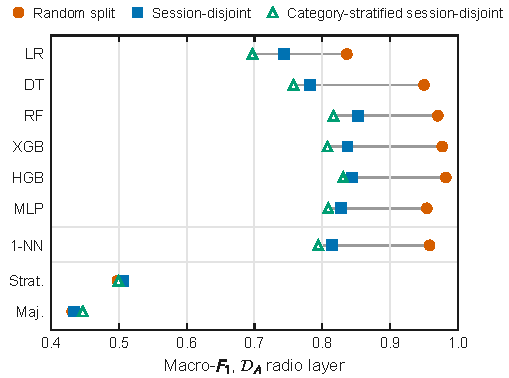
\includegraphics[width=\columnwidth]{../figures/generated/fig_rev_leakage.pdf}
\caption{Macro-$F_1$ on the \DA{} radio layer under three protocols, mean over 20 split seeds; the gray line spans the three protocols of each model. The random split increases the score of every supervised model and of the model-free 1-NN lookup, whereas the scores of the input-blind baselines remain unchanged. Retaining every attack category in training (category-stratified split) does not eliminate the decrease. Corrected intervals are given in Table~\ref{tab:leakage}.}
\label{fig:leakage}
\end{figure}

\begin{table}[t]
\caption{Sequence models on the same radio windows and splits as Table~\ref{tab:leakage}.}
\label{tab:sequence}
\centering
\scriptsize
\setlength{\tabcolsep}{3pt}
%DIF >  GENERATED by analysis/make_tables.py on 2026-09-26
%DIF >  source: EXP-052 sequence_models (EXP-050)
%DIF >  commit: c19230c
%DIF >  DO NOT EDIT. Edit the generator, then re-run `make tables`.
\begin{tabular}{lcccc}
\toprule
Model & Random & Run-disj. & Cat.-strat. & $\Delta_{\mathrm{R-RD}}$ [95\% CI] \\
\midrule
1D-CNN & 0.944 & 0.755 & 0.763 & +0.189 [+0.05, +0.32] \\
GRU & 0.923 & 0.759 & 0.769 & +0.165 [+0.04, +0.29] \\
\bottomrule
\end{tabular}

\end{table}

\subsection{\DIFadd{Time Order and Benign Sessions}}
\label{sec:res:drift}

\DIFadd{Although the radio layer spans \DriftDays{} days, its capture order follows the scenario schedule (Table~\ref{tab:benign}). Nine benign sessions were recorded on days 0 to 6, the five attack categories were recorded in blocks on days 47 to 53, and a final benign session was recorded on day 53. Each session is either benign or belongs to one attack category throughout, so a split by session order holds out entire attack categories. For training fractions between 0.4 }\DIFaddend and \DIFdelbegin \DIFdel{it \emph{tracks model flexibility}: a single depth-12 tree gains most, the boosted ensembles next, the linear model least. The two trivial baselines gain nothing at all, and that is the control which identifies the mechanism. A classifier with no capacity to memorise cannot profit from a leaky split, so the gain is memorisation rather than a change in task difficulty. }%DIFDELCMD < 

%DIFDELCMD < %%%
\DIFdel{The consequence for a reader of this literature is direct: a published random-split score is inflated \emph{most} for exactly the flexible architectures most likely to be published, so the inflation cannot be mentally subtracted as a fixed correction. }\DIFdelend \DIFaddbegin \DIFadd{0.7, the latest sessions contain \DvAuditUnseenMin{} to \DvAuditUnseenMax{} attack categories absent from training, plus a single benign session. Such a split measures the detection of unseen categories, not temporal drift, and we do not report it as a drift estimate.

}\DIFaddend 

\DIFaddbegin \DIFadd{To keep category coverage fixed, we held out the latest session of every category, including the benign category, and compared the result with \DvNctrl{} control draws, each of which holds out a randomly chosen session of every category (Table~\ref{tab:timesplit}). When the latest sessions are held out, balanced accuracy ranges from \DvFwdBAmin{} to \DvFwdBAmax{}, compared with control means of \DvCtrlBAmin{} to \DvCtrlBAmax{}, and yet \DvFwdPctMin\% to \DvFwdPctMax\% of the control draws score equally low. When the earliest sessions are held out, balanced accuracy ranges from \DvRevBAmin{} to \DvRevBAmax{}, a level that \DvRevPctMin\% to \DvRevPctMax\% of the control draws match or exceed. The effect of time order thus remains within the ordinary variation between sessions.

}

\DIFadd{Most of this variation comes from the benign session that lands in the test set. When the benign sessions are held out one at a time (Table~\ref{tab:benign} and Fig.~\ref{fig:benign}), \BenLowN{} of the ten sessions yield a false positive rate of at most \BenLowMax{}, whereas sessions \BenHighSessions{} (days \BenHighDays{}) yield rates between \BenHighMin{} and \BenHighMax{}. The final benign session, the only one recorded during the attack period, yields a false positive rate of \BenLateFPR{} (\BenLateFA{} false alerts per benign UE-hour), but two sessions from the first week yield similar rates. Ten benign sessions cannot separate a change over time from this heterogeneity. The false positive rate of a detector at a new site therefore cannot be inferred from its rate on the benign sessions it was tested on.

}

\DIFaddend \begin{table}[t]
\DIFdelbeginFL %DIFDELCMD < \caption{Evaluation-protocol sensitivity on \DA{} (radio layer). Macro-$F_{1}$ under a random split and under a run-disjoint split, with the paired difference; \measured{20} split seeds, paired $t$-intervals over split means, $^{\ast}$ significant after Holm correction. The two trivial baselines are the control: they gain nothing.}
%DIFDELCMD < \label{tab:indist}
%DIFDELCMD < %%%
\DIFdelendFL \DIFaddbeginFL \caption{False positive rate on each benign radio session when that session alone is held out and the models train on all other 29 sessions, mean and range over the six architectures. Day: capture start relative to the first session. Alerts per benign UE-hour: FPR $\times$ 225 windows.}
\label{tab:benign}
\DIFaddendFL \centering
\DIFdelbeginFL %DIFDELCMD < \footnotesize
%DIFDELCMD < \setlength{\tabcolsep}{4pt}
%DIFDELCMD < %%%
%DIF <  GENERATED by analysis/make_tables.py on 2026-09-21
%DIF <  source: results\EXP-002\processed\leakage_summary.csv
%DIF <  commit: e45aa5b
\DIFdelendFL \DIFaddbeginFL \scriptsize
\setlength{\tabcolsep}{3pt}
%DIF >  GENERATED by analysis/make_tables.py on 2026-09-26
%DIF >  source: EXP-052 drift_v3_benign (EXP-053 C)
%DIF >  commit: c19230c
\DIFaddendFL % DO NOT EDIT. Edit the generator, then re-run `make tables`.
\DIFdelbeginFL %DIFDELCMD < \begin{tabular}{lcccc}
%DIFDELCMD < \toprule
%DIFDELCMD < Model & Random & Run-disjoint & $\Delta$ & 95\,\% CI \\
%DIFDELCMD < \midrule
%DIFDELCMD < rf & 0.970 & 0.853 & +0.117$^{\ast}$ & [+0.057, +0.177] \\
%DIFDELCMD < mlp & 0.959 & 0.849 & +0.110$^{\ast}$ & [+0.056, +0.164] \\
%DIFDELCMD < hgb & 0.982 & 0.844 & +0.138$^{\ast}$ & [+0.082, +0.194] \\
%DIFDELCMD < xgboost & 0.977 & 0.837 & +0.140$^{\ast}$ & [+0.084, +0.195] \\
%DIFDELCMD < tree & 0.950 & 0.782 & +0.168$^{\ast}$ & [+0.110, +0.226] \\
%DIFDELCMD < logreg & 0.836 & 0.744 & +0.093$^{\ast}$ & [+0.037, +0.149] \\
%DIFDELCMD < stratified & 0.498 & 0.507 & -0.009$^{\ast}$ & [-0.011, -0.007] \\
%DIFDELCMD < majority & 0.431 & 0.434 & -0.002 & [-0.008, +0.003] \\
%DIFDELCMD < \bottomrule
%DIFDELCMD < \end{tabular}
%DIFDELCMD < 
%%%
\DIFdelendFL \DIFaddbeginFL \begin{tabular}{rcccccc}
\toprule
Session & Day & UEs & Windows & FPR & Range & Alerts/UE-h \\
\midrule
0 & 0.0 & 1 & 57 & 0.00 & [0.00, 0.00] & 0 \\
1 & 0.0 & 1 & 54 & 0.02 & [0.00, 0.06] & 6 \\
2 & 2.8 & 1 & 58 & 0.00 & [0.00, 0.00] & 0 \\
3 & 2.9 & 1 & 55 & 0.07 & [0.02, 0.20] & 15 \\
4 & 3.0 & 1 & 24 & 0.81 & [0.54, 0.96] & 181 \\
5 & 3.9 & 1 & 56 & 0.14 & [0.00, 0.77] & 31 \\
6 & 4.0 & 2 & 60 & 0.00 & [0.00, 0.00] & 0 \\
7 & 4.0 & 1 & 95 & 0.01 & [0.00, 0.03] & 2 \\
8 & 6.0 & 1 & 56 & 0.98 & [0.93, 1.00] & 220 \\
29 & 52.9 & 3 & 146 & 0.87 & [0.84, 0.93] & 196 \\
\bottomrule
\end{tabular}

\DIFaddendFL 

\end{table}

\DIFdelbegin \subsection{\DIFdel{Cross-Deployment Generalisation}}

%DIFAUXCMD
\addtocounter{subsection}{-1}%DIFAUXCMD
\DIFdelend \DIFaddbegin \begin{table}[t]
\caption{Category-stratified time split on the \DA{} radio layer: balanced accuracy when the latest or the earliest session of every category is held out, against the mean of \DvNctrl{} draws that hold out a random session of every category. ``\% ctrl.\ $\le$'': share of control draws scoring at or below the time split. Every test category is in training.}
\label{tab:timesplit}
\centering
\scriptsize
\setlength{\tabcolsep}{3pt}
%DIF >  GENERATED by analysis/make_tables.py on 2026-09-26
%DIF >  source: EXP-052 drift_v3_compare (EXP-053 B)
%DIF >  commit: c19230c
%DIF >  DO NOT EDIT. Edit the generator, then re-run `make tables`.
\begin{tabular}{lccccc}
\toprule
& Control & \multicolumn{2}{c}{Latest held out} & \multicolumn{2}{c}{Earliest held out} \\
Model & BA & BA & \% ctrl.\ $\le$ & BA & \% ctrl.\ $\le$ \\
\midrule
LR & 0.749 & 0.573 & 20 & 0.950 & 96 \\
DT & 0.774 & 0.521 & 12 & 0.962 & 84 \\
RF & 0.811 & 0.562 & 32 & 0.970 & 66 \\
XGB & 0.812 & 0.567 & 26 & 0.978 & 72 \\
HGB & 0.817 & 0.550 & 32 & 0.995 & 94 \\
MLP & 0.827 & 0.574 & 18 & 0.983 & 94 \\
\bottomrule
\end{tabular}

\DIFaddendFL 

\DIFdelbeginFL \DIFdelFL{Table~\ref{tab:cross} shows what happens when the identical models are applied }\DIFdelendFL \DIFaddbeginFL \end{table}

\begin{figure}[t]
\centering
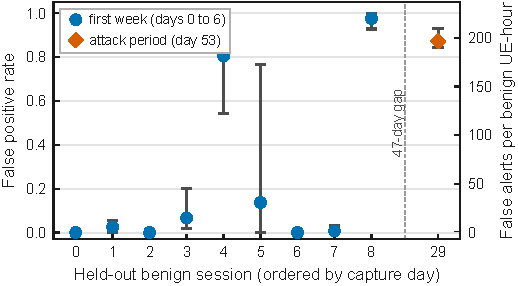
\includegraphics[width=\columnwidth]{../figures/generated/fig_rev_benign.pdf}
\caption{False positive rate on each benign radio session when that session alone is held out: mean (marker) and range (bar) over the six architectures, sessions in capture order. The right axis gives the same rate as false alerts per benign UE-hour (225 windows). Sessions recorded in the same week range from no false positives to almost all windows flagged, which indicates that the false positive rate depends more on the particular benign session than on the time of capture.}
\label{fig:benign}
\end{figure}

\subsection{\DIFadd{The Target Corpus: Labels and a Published Result}}
\label{sec:res:target}

\DIFadd{\emph{Label conflicts.} Before evaluating transfer }\DIFaddend to \DB{}\DIFdelbegin \DIFdel{. Every non-trivial architecture degrades, and all six differences survive Holm correction across the family. That is the less informative }\DIFdelend \DIFaddbegin \DIFadd{, we examined whether its labels are a function of its flow records, and found that this is not the case for }\DIFaddend half of the \DIFdelbegin \DIFdel{result. }%DIFDELCMD < 

%DIFDELCMD < %%%
\DIFdel{The informative half is the floor. A macro-$F_{1}$ of $0.53$ carries no meaning until one knows what guessing scores on the same corpus , and on }\DIFdelend \DIFaddbegin \DIFadd{corpus. Of the \NDbFlows{} flows, \LcShareAll\% (\LcFlowsAll) share every field except the row index, \texttt{Seq}, and \texttt{Offset} with a flow that carries the opposite label (Table~\ref{tab:conflict}, Fig.~\ref{fig:conflict}). All of these flows lie in the two UDP-flood captures, where they account for \LcBenignFileConf\% of file~\LcBenignFile{} and \LcAttackFileConf\% of file~\LcAttackFile{}, one file from each base station. The match is exact. Each of the \LcTwinAttack{} flows labeled as UDP flood in file~\LcAttackFile{} has an identical copy labeled as benign in file~\LcBenignFile{}, and the counts are equal for \LcTwinEqual{} of the \LcTwinRecords{} distinct records. These copies constitute \LcBenignTwinPct\% of the benign class of the corpus. The combined files carry no addresses, but the release of the corpus with all fields preserved does, and it aligns with them row for row. All \LcTwinBenign{} benign copies are UDP flows from }\LcAddrSrc{} \DIFadd{to }\LcAddrDst{}\DIFadd{. The same host pair, protocol, and time window form the flood labeled as attack in file~\LcAttackFile{}, whereas the attack labeled in file~\LcBenignFile{} comes from another host, }\LcAddrOwnSrc{}\DIFadd{, and targets the same address. The capture at the first station thus also recorded the flood of the attacker at the second station, and only its own attacker was labeled. We therefore regard the benign copies as mislabeled attack traffic, which makes the evaluation without them the one with correct labels. We change no label and report every }\DIFaddend \DB{} \DIFdelbegin \DIFdel{a stratified random classifier scores }%DIFDELCMD < \measured{0.4240}%%%
\DIFdel{. The best architecture clears that by }%DIFDELCMD < \measured{0.148}%%%
\DIFdel{; the MLP scores }%DIFDELCMD < \measured{0.4223}%%%
\DIFdel{, which is \emph{beneath} the floor, with }\DIFdelend \DIFaddbegin \DIFadd{result both with and without the copies.

}

\DIFadd{These conflicts cap the performance of any classifier that reads the record content. Even on the flows it was built from, the best possible function of the \LcNFeat{} content fields reaches }\DIFaddend a balanced accuracy of \DIFdelbegin %DIFDELCMD < \measured{0.4966} %%%
\DIFdel{--- on the wrong side of chance. Trained on one O-RAN deployment and applied to another, it does worse than guessing, and it was the strongest model on held-out source data}\DIFdelend \DIFaddbegin \DIFadd{\LcCeilNative{}. In the 18 shared columns the bound is \LcCeilShared{}, the level reached by DT, XGB, HGB, and the MLP when they are trained and tested on a random split of }\DB{} \DIFadd{(Table~\ref{tab:target_ref}). When \texttt{Seq} and \texttt{Offset} are added, every record becomes unique and the bound rises to \LcCeilPos{}}\DIFaddend .

\DIFdelbegin \DIFdel{That last observation generalises. The architecture ranked first on the source ranks \emph{last of six} on the target, and across the six the rank correlation between in-distribution and transfer performance is not significant (Spearman $\rho = \measured{0.143}$, $p = \measured{0.787}$). A practitioner selecting an architecture by its published in-distribution score therefore has close to no information about how it will transfer --- a stronger statement than the usual observation that scores drop. }\DIFdelend \DIFaddbegin \DIFadd{\emph{References within the target.} To separate the cost of transfer from the limits of }\DB{} \DIFadd{itself, we also trained and tested the six architectures on }\DB{} \DIFadd{alone (Table~\ref{tab:target_ref}). On a random split, they reach \TgtRandShBAmin{} to \TgtRandShBAmax{} in the shared space, the bound given above, and \TgtRandShCleanBAmin{} to \TgtRandShCleanBAmax{} when the benign copies are excluded from the test set. On held-out capture files, they reach \TgtFileShBAmin{} to \TgtFileShBAmax{} in the shared space and \TgtFileNatBAmin{} to \TgtFileNatBAmax{} with native features, although none of the three draws held out a UDP-flood capture. Across the two base stations, within a single corpus and with a single exporter, balanced accuracy decreases to \TgtSiteABShBAmin{} to \TgtSiteABShBAmax{} from station 1 to station 2 and to \TgtSiteBAShBAmin{} to \TgtSiteBAShBAmax{} in the opposite direction. Both decreases are caused by the copies. A model trained on station 1, where the flood copies are labeled benign, misses the floods of station 2, whereas a model trained on station 2 flags the benign-labeled copies of station 1 and scores \TgtSiteBAShCleanBAmin{} to \TgtSiteBAShCleanBAmax{} when these copies are removed from the test set. On flows whose labels follow from the record content, the shared space separates the classes of }\DB{} \DIFadd{almost perfectly, so the target corpus itself does not limit transfer.

}\DIFaddend 

\begin{table}[t]
\DIFdelbeginFL %DIFDELCMD < \caption{Cross-deployment performance: trained on \DA{}, evaluated once on the whole of \DB{} using the \measured{18}-column shared space. Intervals are paired $t$-intervals over \measured{20} split seeds; $^{\ast}$ marks significance after Holm correction across the six non-trivial architectures. The two trivial baselines are \emph{italicised}: they are the floor, not competitors. $\Delta_{F_{1}}$ is an \textbf{upper bound} spanning an independent deployment \emph{and} an independent exporter.}
%DIFDELCMD < \label{tab:cross}
%DIFDELCMD < %%%
\DIFdelendFL \DIFaddbeginFL \caption{Label conflicts in \DB{} (5G-NIDD). Content: all fields of the published encoding except row index, \texttt{Seq}, \texttt{Offset}, and the labels. Ceiling: balanced accuracy of the best lookup on distinct records, in sample.}
\label{tab:conflict}
\DIFaddendFL \centering
\scriptsize
\setlength{\tabcolsep}{3pt}
%DIF <  GENERATED by analysis/make_tables.py on 2026-09-21
%DIF <  source: results\EXP-026\processed\transfer_summary__a_to_b.csv
%DIF <  commit: e45aa5b
%DIF >  GENERATED by analysis/make_tables.py on 2026-09-26
%DIF >  source: EXP-057 ceilings
%DIF >  commit: c19230c
% DO NOT EDIT. Edit the generator, then re-run `make tables`.
\DIFdelbeginFL %DIFDELCMD < \begin{tabular}{lccccc}
%DIFDELCMD < \toprule
%DIFDELCMD < Model & Source held-out & Target & $\Delta_{F_1}$ & 95\,\% CI & Target PR-AUC \\
%DIFDELCMD < \midrule
%DIFDELCMD < logreg & 0.626 & 0.530 & +0.096$^{\ast}$ & [+0.043, +0.149] & 0.790 \\
%DIFDELCMD < tree & 0.619 & 0.518 & +0.101$^{\ast}$ & [+0.031, +0.171] & 0.629 \\
%DIFDELCMD < rf & 0.701 & 0.572 & +0.129$^{\ast}$ & [+0.052, +0.207] & 0.654 \\
%DIFDELCMD < xgboost & 0.646 & 0.532 & +0.114$^{\ast}$ & [+0.054, +0.173] & 0.656 \\
%DIFDELCMD < hgb & 0.647 & 0.537 & +0.111$^{\ast}$ & [+0.053, +0.169] & 0.670 \\
%DIFDELCMD < mlp & 0.723 & 0.422 & +0.300$^{\ast}$ & [+0.225, +0.376] & 0.663 \\
%DIFDELCMD < \textit{stratified} & 0.494 & 0.424 & +0.070 & [+0.064, +0.076] & 0.607 \\
%DIFDELCMD < \textit{majority} & 0.492 & 0.378 & +0.114 & [+0.112, +0.117] & 0.607 \\
%DIFDELCMD < \bottomrule
%DIFDELCMD < \end{tabular}
%DIFDELCMD < 
%%%
\DIFdelendFL \DIFaddbeginFL \begin{tabular}{lcccccc}
\toprule
Features & Cols & Records & \multicolumn{3}{c}{\% in conflicting records} & BA \\
& & & All & Benign & Attack & ceiling \\
\midrule
Content fields & 90 & 374\,946 & 52.0 & 58.9 & 47.5 & 0.766 \\
Shared space & 18 & 246\,281 & 62.4 & 59.7 & 64.1 & 0.753 \\
Content + \texttt{Seq}, \texttt{Offset} & 92 & 1\,215\,869 & 0.0 & 0.0 & 0.0 & 1.000 \\
\bottomrule
\end{tabular}

\DIFaddendFL 

\end{table}
\DIFdelbegin %DIFDELCMD < 

%DIFDELCMD < %%%
\DIFdelend \begin{figure}[t]
\centering
\DIFdelbeginFL %DIFDELCMD < 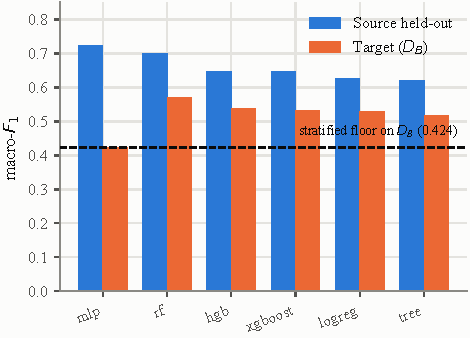
\includegraphics[width=\columnwidth]{../figures/generated/fig_transfer.pdf}
%DIFDELCMD < \caption{The gap a single-corpus evaluation hides, and the line that makes it readable. Bars are macro-$F_1$ on held-out \DA{} and on \DB{}, over \measured{20} split seeds. The dashed line is what a stratified random classifier scores on \DB{}. Architectures are ordered by their \emph{source} score: the leftmost is the best model in distribution and the worst under transfer, landing beneath the floor.}
%DIFDELCMD < \label{fig:gen}
%DIFDELCMD < %%%
\DIFdelendFL \DIFaddbeginFL \resizebox{\columnwidth}{!}{% ---------------------------------------------------------------------------
%  FIGURE -- the label-conflict mechanism in 5G-NIDD (Section VI-C).
%
%  Drawn at print size for one column; every number is a macro from
%  tables/generated/numbers.tex (EXP-055, EXP-057), so nothing is typed by hand.
%  The tile pattern is schematic: the content tiles are identical in the two
%  rows because the records are identical in all 90 content fields; the two
%  position tiles differ because Seq and Offset differ. No field value is shown.
% ---------------------------------------------------------------------------
\fontfamily{phv}\selectfont
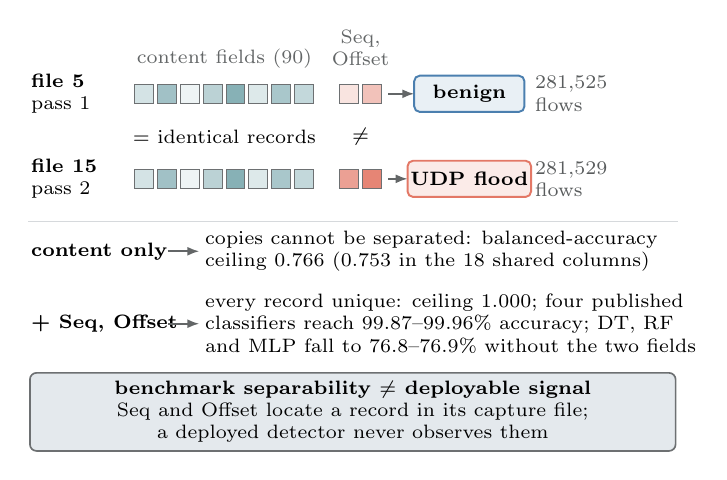
\begin{tikzpicture}[figbase, font=\scriptsize, x=1cm, y=1cm,
  tileC/.style={draw=fInk!70, line width=0.35pt, minimum size=2.4mm, inner sep=0pt},
  chipB/.style={draw=fBlue, fill=fBlue!12, rounded corners=2pt, line width=0.7pt,
                minimum width=14mm, minimum height=4.6mm, font=\scriptsize\bfseries},
  chipA/.style={draw=fCor, fill=fCor!15, rounded corners=2pt, line width=0.7pt,
                minimum width=14mm, minimum height=4.6mm, font=\scriptsize\bfseries},
  arr/.style  ={-{Latex[length=1.5mm]}, draw=fInk!75, line width=0.6pt},
]
% identical content pattern (schematic), and two different position pairs
\def\shades{25,55,10,40,70,20,50,35}
\newcommand{\fcRecord}[3]{% y, first position shade, second position shade
  \foreach \s [count=\i] in \shades
    {\node[tileC, fill=fTeal!\s] at ({1.42+0.29*(\i-1)},#1) {};}
  \node[tileC, fill=fCor!#2] at (4.02,#1) {};
  \node[tileC, fill=fCor!#3] at (4.31,#1) {};}

\node[text=fInk!75] at (2.44,4.86) {content fields (90)};
\node[text=fInk!75, align=center] at (4.17,5.00) {Seq,\\Offset};

% row A: capture file 5, labelled benign
\node[anchor=west, align=left] at (-0.05,4.42) {\textbf{file \LcBenignFile}\\pass 1};
\fcRecord{4.42}{20}{45}
\node[chipB] (lb) at (5.55,4.42) {benign};
\draw[arr] (4.52,4.42) -- (lb.west);
\node[anchor=west, align=left, text=fInk!80] at (6.35,4.42) {\LcTwinBenign{}\\flows};

% row B: capture file 15, labelled UDP flood
\node[anchor=west, align=left] at (-0.05,3.34) {\textbf{file \LcAttackFile}\\pass 2};
\fcRecord{3.34}{70}{90}
\node[chipA] (la) at (5.55,3.34) {UDP flood};
\draw[arr] (4.52,3.34) -- (la.west);
\node[anchor=west, align=left, text=fInk!80] at (6.35,3.34) {\LcTwinAttack{}\\flows};

% between the rows: same content, different position
\node[fill=white, inner sep=1pt] at (2.44,3.88) {$=$ identical records};
\node[fill=white, inner sep=1pt] at (4.17,3.88) {$\neq$};
\draw[draw=fgRule, line width=0.5pt] (-0.05,2.80) -- (8.20,2.80);

% what a classifier can learn from each feature set
\node[anchor=west, font=\scriptsize\bfseries] at (-0.05,2.42) {content only};
\draw[arr] (1.72,2.42) -- (2.12,2.42);
\node[anchor=west, align=left] at (2.16,2.42)
     {copies cannot be separated: balanced-accuracy\\ceiling \LcCeilNative{} (\LcCeilShared{} in the 18 shared columns)};
\node[anchor=west, font=\scriptsize\bfseries] at (-0.05,1.50) {+ Seq, Offset};
\draw[arr] (1.72,1.50) -- (2.12,1.50);
\node[anchor=west, align=left] at (2.16,1.50)
     {every record unique: ceiling \LcCeilPos{}; four published\\classifiers reach \PubRzAccMin--\PubRzAccMax\% accuracy; DT, RF\\and MLP fall to \PubOneNoposAccMin--\PubOneNoposAccMax\% without the two fields};

% the conclusion
\node[draw=fInk!70, rounded corners=2.4pt, line width=0.6pt, fill=fRicI,
      align=center, inner sep=3pt, minimum width=82mm] at (4.07,0.38)
     {\textbf{benchmark separability $\neq$ deployable signal}\\
      Seq and Offset locate a record in its capture file;\\
      a deployed detector never observes them};
\end{tikzpicture}
}
\caption{Illustration of the label conflict in \DB{}. Identical flow records occur in two capture files from the two passes and are labeled benign in one file and UDP flood in the other (the tiles are schematic). Because no function of the record content can separate the copies, the attainable balanced accuracy is bounded. The record-position fields \texttt{Seq} and \texttt{Offset} differ between the copies, make every record unique, and account for the published accuracy of 99.9\%, although a deployed detector cannot observe them.}
\label{fig:conflict}
\DIFaddendFL \end{figure}
\DIFaddbegin \begin{table*}[t]
\caption{References inside \DB{}: balanced accuracy of models trained and tested on \DB{} only, mean over $n$ draws of a 240,000-flow training sample. $^{\ast}$Range over the six architectures on the test flows without the benign copies of Table~\ref{tab:conflict}. Capture-file draws hold out four of the 20 files.}
\label{tab:target_ref}
\centering
\footnotesize
%DIF >  GENERATED by analysis/make_tables.py on 2026-09-26
%DIF >  source: EXP-052 target_reference (EXP-054)
%DIF >  commit: c19230c
%DIF >  DO NOT EDIT. Edit the generator, then re-run `make tables`.
\begin{tabular}{llcccccccc}
\toprule
Features & Split & LR & DT & RF & XGB & HGB & MLP & BA$^{\ast}$ & $n$ \\
\midrule
Shared (18) & Random & 0.708 & 0.752 & 0.723 & 0.752 & 0.752 & 0.750 & 0.84--0.92 & 3 \\
Shared (18) & Capture file & 0.955 & 0.982 & 0.940 & 0.943 & 0.956 & 0.931 & 0.93--0.98 & 3 \\
Shared (18) & Station 1 to 2 & 0.618 & 0.638 & 0.640 & 0.641 & 0.640 & 0.635 & 0.62--0.64 & 1 \\
Shared (18) & Station 2 to 1 & 0.639 & 0.648 & 0.648 & 0.648 & 0.648 & 0.650 & 0.97--0.99 & 1 \\
Native & Random & 0.710 & 0.764 & 0.735 & 0.764 & 0.764 & 0.764 & 0.80--0.87 & 2 \\
Native & Capture file & 0.990 & 1.000 & 0.999 & 1.000 & 1.000 & 0.994 & 0.99--1.00 & 2 \\
Native & Station 1 to 2 & 0.698 & 0.661 & 0.662 & 0.662 & 0.662 & 0.662 & 0.66--0.70 & 1 \\
Native & Station 2 to 1 & 0.648 & 0.648 & 0.649 & 0.650 & 0.650 & 0.654 & 0.99--1.00 & 1 \\
\bottomrule
\end{tabular}

\DIFaddendFL 

\DIFdelbeginFL \DIFdelFL{How separable are the two corpora in the shared space? We do not answer this with a covariate-shift statistic of our own, because a stronger answer already exists: Abraheem and Edhirig~\cite{abraheem2026bidirectional} train a classifier to predict \emph{which corpus} a flow came from and reach a balanced accuracy of 0.993 on harmonised features of the same two corpora, a figure that survives correlation alignment and feature filtering. The corpora are trivially separable. That bounds what any transfer measurement between them can mean, }\DIFdelendFL \DIFaddbeginFL \end{table*}
\DIFadd{\emph{A published result under the same ladder.} The dataset authors report binary accuracies of 99.85\% to 99.95\% on a random 70/30 split~\cite{samarakoon2022niddarxiv}. We reproduced their pipeline, which consists of the published one-hot encoding, selection of the ten features with the highest ANOVA $F$-scores, $z$-score normalization, and their five classifiers, for which we used the scikit-learn default settings because the tuned values are not reported. Our $F$-scores rank the features in exactly the same order, and on their split we obtain accuracies of \PubRzAccMin\% to \PubRzAccMax\% for DT, RF, KNN, and the MLP (Naive Bayes \PubRzAccNB\%), in agreement with their results (Table~\ref{tab:ladder}). Their first and second features are \texttt{Seq} }\DIFaddend and \DIFdelbegin \DIFdel{it is }\DIFdelend \DIFaddbegin \DIFadd{\texttt{Offset}, which encode the position of a record within its capture file. A deployed detector cannot observe these fields, and, according to the bounds given above, they are what separates the conflicting records. Replacing only these two fields with the next two features in their ranking reduces the accuracy of DT, RF, and the MLP to \PubOneNoposAccMin\% to \PubOneNoposAccMax\% (balanced accuracy \PubOneNoposBAmin{} to \PubOneNoposBAmax{}, false positive rate \PubOneNoposFPRmin{} to \PubOneNoposFPRmax). This decrease reflects the label conflict rather than a loss of attack information, since RF still achieves \PubOneRFclean{} on }\DIFaddend the \DIFdelbegin \DIFdel{quantitative form of the exporter confound declared in Section~\ref{sec:setup}. }\DIFdelend \DIFaddbegin \DIFadd{test flows without the benign copies. The two counters thus allow the published models to distinguish identical records by their position within the file. When capture files are held out, the published features yield average balanced accuracies of \PubTwoPubBAmin{} to \PubTwoPubBAmax{} for DT, RF, and the MLP, with RF ranging from \PubTwoPubFoldMin{} to \PubTwoPubFoldMax{} across folds. Without the counters, the average is \PubTwoNoposBAmin{} to \PubTwoNoposBAmax{}, RF ranges from \PubTwoNoposFoldMin{} to \PubTwoNoposFoldMax{}, and accuracy falls to \PubTwoNoposFoldAccMin\% on the fold that tests one flood capture after training on the other. Across base stations, the published features yield \PubThreePubBAmin{} to \PubThreePubBAmax{}, and the features without counters yield \PubThreeNoposBAmin{} to \PubThreeNoposBAmax{}. A published accuracy of 99.9\% on this corpus says little about a new capture file or base station, and nothing about a deployment, where record positions do not exist.
}\begin{table*}[t]
\caption{The 5G-NIDD authors' pipeline~\cite{samarakoon2022niddarxiv} reproduced and moved one step per rung: balanced accuracy on \DB{}. R0 is their protocol. $^{\ast}$RF on the test flows without the benign copies of Table~\ref{tab:conflict}. KNN is evaluated at R0 only.}
\label{tab:ladder}
\centering
\footnotesize
%DIF >  GENERATED by analysis/make_tables.py on 2026-09-26
%DIF >  source: EXP-052 published_ladder (EXP-055)
%DIF >  commit: c19230c
%DIF >  DO NOT EDIT. Edit the generator, then re-run `make tables`.
\begin{tabular}{lllccccccc}
\toprule
& & & \multicolumn{5}{c}{Balanced accuracy} & \multicolumn{2}{c}{RF} \\
Rung & Split & Features & DT & RF & KNN & NB & MLP & BA$^{\ast}$ & FPR \\
\midrule
R0 & Random 70/30 & Published 10 & 0.9995 & 0.9996 & 0.9988 & 0.9310 & 0.9986 & 0.9997 & 0.0005 \\
R1 & Random 70/30 & No \texttt{Seq}/\texttt{Offset} & 0.7059 & 0.7059 & -- & 0.6814 & 0.7042 & 0.9999 & 0.5881 \\
R2 & Capture file & Published 10 & 0.8594 & 0.9226 & -- & 0.7501 & 0.8669 & 0.9578 & 0.0723 \\
R2 & Capture file & No \texttt{Seq}/\texttt{Offset} & 0.7988 & 0.7996 & -- & 0.7593 & 0.8004 & 0.8958 & 0.1937 \\
R3 & Base station & Published 10 & 0.7619 & 0.8949 & -- & 0.6598 & 0.8577 & 0.9354 & 0.0819 \\
R3 & Base station & No \texttt{Seq}/\texttt{Offset} & 0.6557 & 0.6555 & -- & 0.6271 & 0.6919 & 0.8284 & 0.3465 \\
\bottomrule
\end{tabular}

\DIFaddendFL 

\DIFdelbeginFL \DIFdelFL{The reverse direction, }%DIFDELCMD < \DB{} %%%
\DIFdelFL{to }%DIFDELCMD < \DA{}%%%
\DIFdelFL{, is reported separately as a symmetry check rather than as a second headline. It distinguishes ``detectors do not transfer'' from ``}\DIFdelendFL \DIFaddbeginFL \end{table*}
\subsection{\DIFadd{Transfer Across Corpora}}
\label{sec:res:transfer}

\DIFadd{Table~\ref{tab:transfer} and Fig.~\ref{fig:transfer} report the results of transfer from }\DA{} \DIFadd{to }\DIFaddend \DB{}\DIFdelbegin \DIFdel{is simply harder'', and it carries a caveat the forward direction does not: }%DIFDELCMD < \DB{} %%%
\DIFdel{publishes no identifiers, so it has no group key, and its own }\DIFdelend \DIFaddbegin \DIFadd{. In terms of macro-$F_1$, every supervised model loses \TrFoneDropMin{} to \TrFoneDropMax{}. However, the majority baseline, which uses no features, also loses \TrMajDrop{}, because }\DB{} \DIFadd{has a lower attack prevalence than }\DA{}\DIFadd{. Relative to this baseline, the loss in macro-$F_1$ lies between \TrDiDmin{} and \TrDiDmax{}, and none of the macro-$F_1$ losses remains significant after correction. Macro-$F_1$ is the wrong measure for this comparison. Balanced accuracy, which prevalence does not affect, shows the loss clearly. It decreases from \TrSrcBAmin{}--\TrSrcBAmax{} on }\DIFaddend held-out \DIFdelbegin \DIFdel{reference is a random split and therefore an optimistic bound. Its $\Delta_{F_{1}}$ is consequently an over-estimate. }%DIFDELCMD < 

%DIFDELCMD < %%%
\DIFdel{We do not report a fine-tuning result. Few-shot adaptation on labelled target data is a different experiment, it is already published for these corpora~\cite{abraheem2026bidirectional}, and it relocates the problem rather than solving it: it means each deployment requires its own labelled attack data, which is exactly the cost a pre-trained detection xApp was supposed to avoid}\DIFdelend \DIFaddbegin \DIFadd{source data to \TrTgtBAmin{}--\TrTgtBAmax{} on }\DB{}\DIFadd{, a drop of \TrBAdropMin{} to \TrBAdropMax{} that is significant for \TrSigBA{} of the six architectures after correction, is positive in at least \TrBAseedsMin{} of the 20 splits for every architecture, and averages \TrBAdropAvg{} }[\DIFadd{\TrBAdropAvgNbLo, \TrBAdropAvgNbHi}]\DIFadd{. The trivial baselines remain unchanged, and the target ROC-AUC lies between \TrTgtAUCmin{} and \TrTgtAUCmax{}}\DIFaddend .

The \DIFdelbegin \DIFdel{degradation is statistically unambiguous. A paired $t$-test over }%DIFDELCMD < \measured{20} %%%
\DIFdel{split seeds rejects the null hypothesis of equal held-out and cross-deployment }\DIFdelend \DIFaddbegin \DIFadd{detectors stay above chance on the target, but not by much. The average target balanced accuracy is \TrTgtBAavg{}, and the corrected interval excludes 0.5 for \TrChanceSig{} of the six architectures (\TrChanceSigHolm{} after Holm correction). For reference, the stratified sampler achieves a }\DIFaddend macro-\DIFdelbegin \DIFdel{$F_{1}$ for **all six** non-trivial architectures , and every one survives Holm correctionacross the family ($p_{\text{Holm}} \le \measured{0.0069}$). Effect sizes are large, with $d_{z}$ between }%DIFDELCMD < \measured{0.68} %%%
\DIFdel{and }%DIFDELCMD < \measured{1.86}%%%
\DIFdel{. }%DIFDELCMD < 

%DIFDELCMD < %%%
\DIFdel{The choice among detector families is a second-order effect beside the shared failure to transfer, and this is the more useful way to read the table: the spread across architectures on the target, }%DIFDELCMD < \measured{0.149} %%%
\DIFdel{of }\DIFdelend \DIFaddbegin \DIFadd{$F_1$ of \TrStratFloor{} on }\DB{}\DIFadd{, and a fair coin would achieve \TrFairCoin{}. We give both because a }\DIFaddend macro-\DIFdelbegin \DIFdel{$F_{1}$ from best to worst, is smaller than the distance any of them has fallen, and }\DIFdelend \DIFaddbegin \DIFadd{$F_1$ floor depends on the prior it samples from. According to every prevalence-independent measure, LR transfers best (balanced accuracy \TrLRtgtBA{}, ROC-AUC \TrLRtgtAUC{}), whereas the MLP, which achieves the highest held-out source balanced accuracy (\TrMLPsrcBA{}), reaches \TrMLPtgtBA{} on the target. Source performance does not predict target performance in a prevalence-independent metric: across the six architectures }\DIFaddend the \DIFdelbegin \DIFdel{ordering is not the source ordering. }\DIFdelend \DIFaddbegin \DIFadd{rank correlation in balanced accuracy is \RhoBA{} ($p=\RhoBAP$). In macro-$F_1$ the rank correlation is \RhoFone{} ($p=\RhoFoneP$), but rankings in macro-$F_1$ change with prevalence, and six architectures provide little precision for either estimate.

}\DIFaddend 

\DIFdelbegin \DIFdel{A single aggregate score conceals the shape of }\DIFdelend \DIFaddbegin \DIFadd{\emph{Effect of the target labels.} Part of this loss comes from the label conflict of Section~\ref{sec:res:target}. Detectors that learned to recognize a UDP flood on }\DA{} \DIFadd{detect the floods in capture file~\LcAttackFile{} and, by the same rule, flag between \NetCopyFlagMin{} and \NetCopyFlagMax{} of the benign-labeled copies in file~\LcBenignFile{}, whereas LR detects neither. When the copies are excluded, in a deterministic re-run of 10 of the 20 split seeds, }\DIFaddend the \DIFdelbegin \DIFdel{failure, so Table~\ref{tab:percat} reports detection per attack category on the target . The benign column is specificity; the remainder are recall. }\DIFdelend \DIFaddbegin \DIFadd{target balanced accuracy is \TrCleanTgtBAmin{} to \TrCleanTgtBAmax{} (\TrCleanOthMin{} to \TrCleanOthMax{} for the five nonlinear architectures and \TrCleanLR{} for LR). The loss relative to held-out source data decreases to \TrCleanDropMin{} to \TrCleanDropMax{} and is significant for \TrCleanSig{} of the six architectures after correction. The conflicts reverse the apparent ranking. On all flows LR seems to transfer best, and on the flows with consistent labels it is the worst. Compared with the in-target reference on these flows (Table~\ref{tab:target_ref}), transfer still falls short by \TrCleanShortMin{} to \TrCleanShortMax{} in balanced accuracy.

}\DIFaddend 

\DIFdelbegin \DIFdel{\textbf{No architecture is usable on both classes.} Logistic regression holds }%DIFDELCMD < \measured{0.977} %%%
\DIFdel{benign specificity and detects }%DIFDELCMD < \measured{0.247} %%%
\DIFdel{of the denial-of-service traffic. The MLP detects }%DIFDELCMD < \measured{0.884} %%%
\DIFdel{of it, and }%DIFDELCMD < \measured{0.807} %%%
\DIFdel{of the scanning traffic, while classifying }%DIFDELCMD < \measured{0.885} %%%
\DIFdel{of benign traffic as attack --- which is why its macro-$F_1$ falls beneath the trivial floor. The tree ensembles occupy a middle position and are the weakest at scanning, recovering }%DIFDELCMD < \measured{0.168} %%%
\DIFdel{to }%DIFDELCMD < \measured{0.295} %%%
\DIFdel{of it.

}\DIFdelend \DIFaddbegin \begin{table*}[t]
\caption{Transfer from \DA{} to \DB{} in the 18-column shared space, mean over 20 split seeds. $\Delta_{\mathrm{BA}}$: source minus target balanced accuracy, with Nadeau--Bengio corrected 95\% interval; $^{\ast}$: significant after Holm correction. Last column: macro-$F_1$ loss minus the majority baseline's loss. Italic rows are the trivial baselines.}
\label{tab:transfer}
\centering
\footnotesize
%DIF >  GENERATED by analysis/make_tables.py on 2026-09-26
%DIF >  source: EXP-052 transfer_stats (EXP-041)
%DIF >  commit: c19230c
%DIF >  DO NOT EDIT. Edit the generator, then re-run `make tables`.
\begin{tabular}{lccccccc}
\toprule
& \multicolumn{2}{c}{Macro-$F_1$} & \multicolumn{3}{c}{Balanced accuracy} & Target & $\Delta_{F_1}$ vs. \\
Model & Src. & Tgt. & Src. & Tgt. & $\Delta_{\mathrm{BA}}$ [95\% CI] & ROC-AUC & Maj. \\
\midrule
LR & 0.626 & 0.530 & 0.837 & 0.627 & +0.210$^{\ast}$ [+0.10, +0.32] & 0.701 & -0.018 \\
DT & 0.619 & 0.518 & 0.822 & 0.533 & +0.290$^{\ast}$ [+0.08, +0.50] & 0.526 & -0.013 \\
RF & 0.701 & 0.572 & 0.808 & 0.581 & +0.227 [-0.01, +0.47] & 0.578 & +0.015 \\
XGB & 0.646 & 0.532 & 0.864 & 0.562 & +0.303$^{\ast}$ [+0.14, +0.47] & 0.572 & -0.001 \\
HGB & 0.647 & 0.537 & 0.867 & 0.566 & +0.301$^{\ast}$ [+0.13, +0.47] & 0.581 & -0.004 \\
MLP & 0.655 & 0.531 & 0.912 & 0.553 & +0.359$^{\ast}$ [+0.22, +0.50] & 0.557 & +0.010 \\
\textit{Strat.} & 0.494 & 0.424 & 0.502 & 0.500 & +0.001 [-0.01, +0.01] & 0.500 & -0.044 \\
\textit{Maj.} & 0.492 & 0.378 & 0.500 & 0.500 & +0.000 [+0.00, +0.00] & 0.500 & +0.000 \\
\bottomrule
\end{tabular}

\DIFaddendFL 

\DIFdelbeginFL \DIFdelFL{This is not a smooth degradation in which every detector gets uniformly worse.

Each architecture fails differently}\DIFdelendFL \DIFaddbeginFL \end{table*}

\begin{figure}[t]
\centering
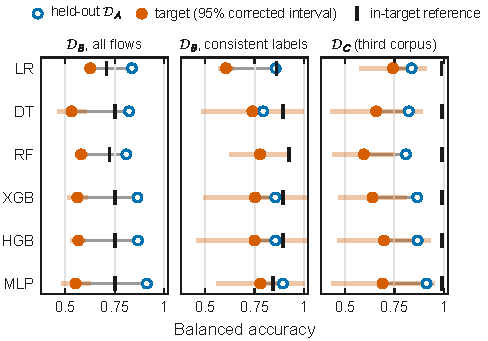
\includegraphics[width=\columnwidth]{../figures/generated/fig_rev_transfer.pdf}
\caption{Balanced accuracy of detectors trained on \DA{}: on held-out \DA{} (open) and on the target (filled, with the Nadeau--Bengio corrected 95\% interval), for \DB{} on all flows (20 split seeds), \DB{} without the benign copies of Fig.~\ref{fig:conflict} (10 seeds), and the third corpus \DC{} (20 seeds). The vertical bar is a reference trained and tested inside the target on a random split. The dashed line is chance, where both input-blind baselines sit. On every target the transferred detectors fall short of the in-target reference.}
\label{fig:transfer}
\end{figure}

\DIFadd{The reverse direction (Table~\ref{tab:transfer_rev}) behaves differently. Balanced accuracy on }\DA{} \DIFadd{reaches \TrRevTgtBAmin{} to \TrRevTgtBAmax{}}\DIFaddend , and the \DIFdelbegin \DIFdel{difference is not visible in any single number. }%DIFDELCMD < 

%DIFDELCMD < %%%
\DIFdel{The reverse direction makes the mechanism explicit, }\DIFdelend \DIFaddbegin \DIFadd{change relative to the source reference, which is optimistic because it is based on a random split, ranges from \TrRevBAdropMin{} to \TrRevBAdropMax{}. LR, XGB, HGB, and the MLP lose little or no balanced accuracy, whereas DT and RF lose a significant amount. Macro-$F_1$ nevertheless decreases sharply, }\DIFaddend because \DA{} \DIFdelbegin \DIFdel{contains every category }\DIFdelend \DIFaddbegin \DIFadd{consists of \PrevDa\% attack traffic and a small number of false negatives dominates the small benign class. A model trained on the narrower }\DIFaddend \DB{} \DIFdelbegin \DIFdel{does and four more, so nothing is untestable. Categories present in the training corpus transfer: the boosted ensembles recover }%DIFDELCMD < \measured{0.83} %%%
\DIFdel{to }%DIFDELCMD < \measured{0.87} %%%
\DIFdel{of distributed denial of service and }%DIFDELCMD < \measured{0.87} %%%
\DIFdel{to }%DIFDELCMD < \measured{0.89} %%%
\DIFdel{of scanning. Categories absent from it do not. }\DIFdelend \DIFaddbegin \DIFadd{separates the classes of }\DA{} \DIFadd{better than a model trained on }\DA{} \DIFadd{separates those of }\DIFaddend \DB{}\DIFdelbegin \DIFdel{contains no }\DIFdelend \DIFaddbegin \DIFadd{. One untested explanation is that the larger and more varied benign traffic of }\DB{} \DIFadd{gives a better model of benign behavior.

}

\begin{table}[t]
\caption{Reverse direction, \DB{} to \DA{}. The source reference is a random split of \DB{}, which has no group key, and is therefore optimistic.}
\label{tab:transfer_rev}
\centering
\scriptsize
\setlength{\tabcolsep}{2.2pt}
%DIF >  GENERATED by analysis/make_tables.py on 2026-09-26
%DIF >  source: EXP-052 transfer_stats (EXP-041)
%DIF >  commit: c19230c
%DIF >  DO NOT EDIT. Edit the generator, then re-run `make tables`.
\begin{tabular}{lccccccc}
\toprule
& \multicolumn{2}{c}{Macro-$F_1$} & \multicolumn{3}{c}{Balanced accuracy} & Target & $\Delta_{F_1}$ vs. \\
Model & Src. & Tgt. & Src. & Tgt. & $\Delta_{\mathrm{BA}}$ [95\% CI] & ROC-AUC & Maj. \\
\midrule
LR & 0.708 & 0.563 & 0.708 & 0.745 & -0.037$^{\ast}$ [-0.05, -0.02] & 0.827 & +0.254 \\
DT & 0.752 & 0.343 & 0.751 & 0.607 & +0.145$^{\ast}$ [+0.05, +0.24] & 0.622 & +0.518 \\
RF & 0.730 & 0.337 & 0.723 & 0.630 & +0.093$^{\ast}$ [+0.06, +0.13] & 0.845 & +0.502 \\
XGB & 0.753 & 0.497 & 0.752 & 0.764 & -0.012 [-0.03, +0.01] & 0.845 & +0.364 \\
HGB & 0.753 & 0.488 & 0.752 & 0.751 & +0.001 [-0.05, +0.05] & 0.832 & +0.373 \\
MLP & 0.752 & 0.470 & 0.751 & 0.728 & +0.023 [-0.04, +0.09] & 0.814 & +0.390 \\
\textit{Strat.} & 0.502 & 0.417 & 0.502 & 0.500 & +0.003 [+0.00, +0.00] & 0.500 & +0.194 \\
\textit{Maj.} & 0.377 & 0.486 & 0.500 & 0.500 & +0.000 [+0.00, +0.00] & 0.500 & +0.000 \\
\bottomrule
\end{tabular}

\end{table}

\DIFadd{Per-category detection (Table~\ref{tab:percat}) shows that no architecture performs acceptably on both classes of }\DB{}\DIFadd{. LR keeps a benign specificity of \FwdLRspec{} but detects only \FwdLRdos{} of the DoS traffic. The tree models and the MLP detect more attacks and flag \FwdEnsFlagMin{} to \FwdEnsFlagMax{} of the benign traffic. In the reverse direction, categories absent from }\DB{} \DIFadd{are detected unevenly. The ensembles and the MLP recall at most \RevWebEnsMax{} of the }\DIFaddend web attacks, \DIFdelbegin \DIFdel{and web recall on }%DIFDELCMD < \DA{} %%%
\DIFdel{is between }%DIFDELCMD < \measured{0.004} %%%
\DIFdel{and }%DIFDELCMD < \measured{0.013} %%%
\DIFdel{for four of six architectures.

A detector does not recognise an attack class it has never been shown, and it fails silently rather than noisily.

}\DIFdelend \DIFaddbegin \DIFadd{whereas brute-force attacks, which are also absent from }\DB{}\DIFadd{, are recalled at rates of \RevBFmin{} to \RevBFmax.

}\DIFaddend 

\DIFdelbegin %DIFDELCMD < \begin{table}[t]
%DIFDELCMD < \caption{Per-category detection on \DB{}, trained on \DA{}. Mean over \measured{20} split seeds at $\tau=0.5$. The \texttt{benign} column is specificity; the others are recall. \DB{} contains no DDoS, brute-force or web traffic, so those three categories are \emph{untestable} in this direction and are omitted rather than averaged in as though they had been evaluated.}
%DIFDELCMD < %%%
\DIFdelendFL \DIFaddbeginFL \begin{table*}[t]
\caption{Per-category detection, mean over 20 split seeds at $\tau=0.5$. ``Ben.'' is specificity; other columns are recall. BF: brute force. Categories absent from \DB{} can be tested only in the reverse direction.}
\DIFaddendFL \label{tab:percat}
\centering
\footnotesize
%DIF <  GENERATED by analysis/make_tables.py on 2026-09-21
%DIF <  source: results\EXP-026\processed\per_category_recall__a_to_b.csv
%DIF <  commit: e45aa5b
%DIF >  GENERATED by analysis/make_tables.py on 2026-09-26
%DIF >  source: EXP-041 per_category_recall (both directions)
%DIF >  commit: c19230c
% DO NOT EDIT. Edit the generator, then re-run `make tables`.
\DIFdelbeginFL %DIFDELCMD < \begin{tabular}{lccc}
%DIFDELCMD < \toprule
%DIFDELCMD < Model & benign & dos & probe \\
%DIFDELCMD < \midrule
%DIFDELCMD < logreg & 0.977 & 0.247 & 0.645 \\
%DIFDELCMD < tree & 0.442 & 0.651 & 0.295 \\
%DIFDELCMD < rf & 0.459 & 0.745 & 0.191 \\
%DIFDELCMD < xgboost & 0.571 & 0.584 & 0.168 \\
%DIFDELCMD < hgb & 0.537 & 0.630 & 0.183 \\
%DIFDELCMD < mlp & 0.115 & 0.884 & 0.807 \\
%DIFDELCMD < \bottomrule
%DIFDELCMD < \end{tabular}
%DIFDELCMD < 
%%%
\DIFdelendFL \DIFaddbeginFL \begin{tabular}{lccc|cccccc}
\toprule
& \multicolumn{3}{c|}{\DA{}$\rightarrow$\DB{}} & \multicolumn{6}{c}{\DB{}$\rightarrow$\DA{} (absent from \DB{}: DDoS, BF, web)} \\
Model & Ben. & DoS & Probe & Ben. & DoS & Probe & DDoS & BF & Web \\
\midrule
LR & 0.98 & 0.25 & 0.64 & 0.71 & 0.85 & 0.92 & 0.96 & 0.57 & 0.30 \\
DT & 0.44 & 0.65 & 0.29 & 0.82 & 0.44 & 0.47 & 0.48 & 0.43 & 0.13 \\
RF & 0.46 & 0.74 & 0.19 & 0.89 & 0.41 & 0.55 & 0.49 & 0.34 & 0.00 \\
XGB & 0.57 & 0.58 & 0.17 & 0.89 & 0.73 & 0.88 & 0.85 & 0.35 & 0.01 \\
HGB & 0.54 & 0.63 & 0.18 & 0.87 & 0.72 & 0.87 & 0.83 & 0.34 & 0.01 \\
MLP & 0.46 & 0.68 & 0.25 & 0.86 & 0.71 & 0.73 & 0.81 & 0.36 & 0.00 \\
\bottomrule
\end{tabular}

\DIFaddendFL 

\DIFdelbeginFL %DIFDELCMD < \end{table}
%DIFDELCMD < 
%%%
\DIFdelend \DIFaddbegin \end{table*}

\DIFaddend 

\subsection{\DIFdelbegin \DIFdel{Score Calibration and Prior Shift}\DIFdelend \DIFaddbegin \DIFadd{Composition of the Transfer Gap}\DIFaddend }
\DIFdelbegin %DIFDELCMD < \label{sec:calibration}
%DIFDELCMD < 
%%%
\DIFdelend \DIFaddbegin \label{sec:res:anatomy}

\DIFaddend 

\DIFdelbegin \DIFdel{All three deployment criteria depend on the score $\hat{p}$ behaving as a probability, because \eqref{eq:ppv} and \eqref{eq:tau} both operate on a threshold applied to it. We therefore report expected calibration error over fifteen \emph{equal-mass} bins; equal-width bins are misleading here, because scores pile up near 1.0 and most equal-width bins are then empty.}\DIFdelend \DIFaddbegin \DIFadd{\emph{Separability.} A classifier trained to distinguish }\DA{} \DIFadd{flows from }\DB{} \DIFadd{flows achieves a balanced accuracy of \DomShared{} on the 18 shared columns and of \DomRobust{} on the nine exporter-robust columns alone. The largest per-feature shifts are in the protocol mix (most }\DA{} \DIFadd{flows are TCP and most }\DB{} \DIFadd{flows are UDP), the direction ratios, and the packet counts (Fig.~\ref{fig:shift}). The robust columns shift as much as the segmentation-dependent columns ($\bar{W}_1$ of \WoneRobust{} compared with \WoneNonrobust). The corpora thus differ in traffic composition, which no choice of exporter would remove, as well as in flow segmentation, which a common exporter would remove.

}\DIFaddend 

\DIFdelbegin \DIFdel{In distribution the models are reasonably calibrated, with ECE between }%DIFDELCMD < \measured{0.028} %%%
\DIFdel{and }%DIFDELCMD < \measured{0.185}%%%
\DIFdel{. Under transfer they are not: target ECE rises to between }%DIFDELCMD < \measured{0.251} %%%
\DIFdel{and }%DIFDELCMD < \measured{0.396}%%%
\DIFdel{. That is }\DIFdelend \DIFaddbegin \DIFadd{\emph{A common exporter.} The raw captures of }\DB{} \DIFadd{are public, so we re-extracted them with Zeek \ZkVersion{}, the exporter of }\DA{}\DIFadd{, and mapped the Zeek records onto the shared space with the same function as those of }\DA{}\DIFadd{. In every capture of }\DB{}\DIFadd{, the published attack flows are the traffic of one host pair. Labeling a flow as attack when its host pair is an attack pair of the same capture reproduces \ZkRuleAgreePct\% of the published labels, and we carried these labels over to the \ZkFlows{} Zeek flows (\ZkAttackPct\% attacks). The flood copies of Section~\ref{sec:res:target} reappear in the Zeek output (\ZkCopies{} flows), so they lie in the captures and are not an artifact of the Argus export. We then repeated the transfer on the same \ZkSeeds{} split seeds as the Argus results without the copies. The trained models are identical, and only the export of the target differs. On all flows, balanced accuracy falls from \ZkArgBAmin{}--\ZkArgBAmax{} with Argus to \ZkBAmin{}--\ZkBAmax{} with Zeek, and the paired difference over seeds (\ZkDiffMin{} to \ZkDiffMax{}) has a 95\% interval below zero for \ZkSigNeg{} of the six architectures. Without the copies, five architectures change by \ZkCleanOthDiffMin{} to \ZkCleanOthDiffMax{}, none of them significantly, and LR loses \ZkCleanLRloss{}. The false positive rate rises under Zeek for every architecture, to \ZkCleanFPRmin{}--\ZkCleanFPRmax{} without the copies against \ZkCleanArgFPRmin{}--\ZkCleanArgFPRmax{} with Argus. A common exporter does not close the gap. What remains is the difference in traffic composition that }\DIFaddend the \DIFdelbegin \DIFdel{expected finding, and it suggested an obvious remedy --- calibrate on held-out source data and recover the operating point. We tested it, and the remedy fails in an instructive way. }%DIFDELCMD < 

%DIFDELCMD < %%%
\DIFdel{Fitting Platt scaling or isotonic regression on a group-disjoint source calibration fold halves both Brier score and ECE, exactly as advertised, and simultaneously makes the operating point far worse. For logistic regression on the source, Brier falls from }%DIFDELCMD < \measured{0.1023} %%%
\DIFdel{to }%DIFDELCMD < \measured{0.0486} %%%
\DIFdel{while deployment PPV falls from }%DIFDELCMD < \measured{0.0174} %%%
\DIFdel{to }%DIFDELCMD < \measured{0.0025} %%%
\DIFdel{and the alert queue grows from }%DIFDELCMD < \measured{35{,}330} %%%
\DIFdel{to }%DIFDELCMD < \measured{216{,}846} %%%
\DIFdel{per hour. A calibrator fitted on a corpus that is }%DIFDELCMD < \measured{94.63}%%%
\DIFdel{\% attack learns to map scores onto that prior, so applied anywhere it pushes almost every score past $\tau=0.5$ and the detector flags nearly everything. }%DIFDELCMD < 

%DIFDELCMD < %%%
\DIFdel{There is a stronger statement available, and it explains why no calibrator could have worked. Every method tested here is a monotone transform, so none changes the model's ranking of examples and none changes the set of achievable operating points. We verify this rather than assert it: Platt and temperature scaling preserve ROC-AUC to within $10^{-5}$ for five of six architectures. **Threshold saturation is therefore not a calibration failure but a discriminability limit. ** Target ROC-AUC lies between }%DIFDELCMD < \measured{0.537} %%%
\DIFdel{and }%DIFDELCMD < \measured{0.691}%%%
\DIFdel{, and no threshold, under any calibration, extracts a usable operating point from a curve that close to the diagonal}\DIFdelend \DIFaddbegin \DIFadd{domain classifier and the robust columns already indicated}\DIFaddend .

\DIFdelbegin \DIFdel{One methodological warning follows, because it nearly produced a positive result from nothing. Temperature scaling appears in our sweep to rescue two architectures that raw scores cannot rescue. It preserves the ROC exactly, so it rescues nothing: it rescales the scores so that a \emph{fixed grid} of swept thresholds lands on a different part of the same curve. Any comparison of monotone calibrators over a fixed threshold grid can manufacture this artefact, and }\DIFdelend \DIFaddbegin \DIFadd{\emph{Model families and adaptation.} Table~\ref{tab:arms} evaluates the same splits under three modifications, none of which yields a transferable detector. Restricting the detectors to }\DIFaddend the \DIFdelbegin \DIFdel{ROC should be reported alongside the grid. }%DIFDELCMD < 

%DIFDELCMD < %%%
\DIFdel{This compounds the earlier findings rather than merely adding to them. The remedy suggested by Fig.~\ref{fig:alerts} --- raising the threshold to suppress alert volume --- assumes that a high score means high confidence, and under transfer it does not, so the operating point chosen on the source deployment does not carry over even in the ordering it induces.

}%DIFDELCMD < 

%DIFDELCMD < %%%
\DIFdel{A second and independent effect is prior shift, and it is severe. Training prevalence on }%DIFDELCMD < \DA{} %%%
\DIFdel{is }%DIFDELCMD < \measured{94.63}%%%
\DIFdel{\%, target prevalence on }%DIFDELCMD < \DB{} %%%
\DIFdel{is }%DIFDELCMD < \measured{60.71}%%%
\DIFdel{\% }\DIFdelend \DIFaddbegin \DIFadd{nine exporter-robust columns raises the held-out source balanced accuracy to \RobSrcBAmin{} to \RobSrcBAmax{}, but the target balanced accuracy falls to \RobBAmin{} to \RobBAmax{}, no better than chance. The columns that do not depend on flow segmentation thus carry the shift in traffic composition. CORAL, which uses unlabeled target features, yields a target balanced accuracy of \CoralBAmin{} to \CoralBAmax{}. Only the MLP benefits from it (\CoralMLPtgtBA{} compared with \TrMLPtgtBA{} without adaptation)}\DIFaddend , and the \DIFdelbegin \DIFdel{operational prevalence assumed in Section~\ref{sec:setup} is $\pi=0.002$. A classifier trained under one prior emits scores calibrated to that prior. Where the training prior $\pi_{\text{tr}}$ is known, the scores admit a closed-form correction,
}%DIFDELCMD < \begin{equation}
%DIFDELCMD < \tilde{p} \;=\; \frac{\hat{p}\,\dfrac{\pi}{\pi_{\text{tr}}}}{\hat{p}\,\dfrac{\pi}{\pi_{\text{tr}}} \;+\; \left(1-\hat{p}\right)\dfrac{1-\pi}{1-\pi_{\text{tr}}}},
%DIFDELCMD < \label{eq:prior}
%DIFDELCMD < \end{equation}
%DIFDELCMD < %%%
\DIFdel{which rescales the decision surface without retraining.

}\DIFdelend \DIFaddbegin \DIFadd{target false positive rate increases to \CoralFPRmin{} to \CoralFPRmax{}. The novelty detectors trained on benign traffic alone already fail on held-out source data, because floods and scans resemble short benign flows in this feature space.

}\DIFaddend 

\DIFdelbegin \DIFdel{We tested this correction and it does not work either, which is worth reporting because it is the obvious next thing to try. Applying \eqref{eq:prior} requires the target prior, which a deployment does not know; we supply the true value anyway, as an oracle, to bound what the correction could achieve. Even so it does not beat leaving the scores alone: for logistic regression, oracle prior correction gives an operational precision of }%DIFDELCMD < \measured{0.0197} %%%
\DIFdel{against }%DIFDELCMD < \measured{0.0221} %%%
\DIFdel{for raw scores. It does cut the alert queue sharply, from }%DIFDELCMD < \measured{19{,}551} %%%
\DIFdel{to }%DIFDELCMD < \measured{3{,}285} %%%
\DIFdel{per hour, by moving to a far more conservative operating point, and it pays for that with more than half the remaining recall }\DIFdelend \DIFaddbegin \DIFadd{\emph{Cost of the shared space.} Projecting }\DA{} \DIFadd{onto the 18 shared columns reduces the in-distribution balanced accuracy by \HarmBAmin{} to \HarmBAmax{} relative to the use of all \NFullFeat{} non-port Zeek features (Table~\ref{tab:harm}). The low source macro-$F_1$ values in Table~\ref{tab:transfer} reflect the \PrevDa\% attack prevalence of }\DA{} \DIFadd{rather than weak detectors, as the corresponding source balanced accuracy is \TrSrcBAmin{} to \TrSrcBAmax}\DIFaddend .

\DIFdelbegin \DIFdel{Prior shift is therefore real, and correcting it helps the queue rather than the precision. It is not the binding constraint. }\DIFdelend \DIFaddbegin \begin{table}[t]
\caption{Transfer from \DA{} to \DB{} under alternative feature sets, adaptation, and model families, mean over 20 split seeds. CORAL reads unlabeled target features.}
\label{tab:arms}
\centering
\scriptsize
\setlength{\tabcolsep}{2.6pt}
%DIF >  GENERATED by analysis/make_tables.py on 2026-09-26
%DIF >  source: EXP-052 arms_summary (EXP-041, 045, 048, 049)
%DIF >  commit: c19230c
%DIF >  DO NOT EDIT. Edit the generator, then re-run `make tables`.
\begin{tabular}{llcccc}
\toprule
Arm & Model & Src.\ BA & Tgt.\ BA & Tgt.\ AUC & Tgt.\ FPR \\
\midrule
Shared space (18) & LR & 0.837 & 0.627 & 0.701 & 0.023 \\
 & DT & 0.822 & 0.533 & 0.526 & 0.558 \\
 & RF & 0.808 & 0.581 & 0.578 & 0.541 \\
 & XGB & 0.864 & 0.562 & 0.572 & 0.429 \\
 & HGB & 0.867 & 0.566 & 0.581 & 0.463 \\
 & MLP & 0.912 & 0.553 & 0.557 & 0.539 \\
\midrule
Exporter-robust subset (9) & LR & 0.804 & 0.510 & 0.583 & 0.854 \\
 & DT & 0.883 & 0.480 & 0.488 & 0.177 \\
 & RF & 0.894 & 0.507 & 0.469 & 0.206 \\
 & XGB & 0.925 & 0.511 & 0.533 & 0.089 \\
 & HGB & 0.939 & 0.521 & 0.541 & 0.090 \\
 & MLP & 0.928 & 0.534 & 0.499 & 0.039 \\
\midrule
CORAL (reads target features) & LR & 0.836 & 0.503 & 0.646 & 0.902 \\
 & DT & 0.812 & 0.500 & 0.504 & 0.870 \\
 & RF & 0.795 & 0.481 & 0.515 & 0.992 \\
 & XGB & 0.906 & 0.473 & 0.478 & 0.906 \\
 & HGB & 0.875 & 0.481 & 0.484 & 0.915 \\
 & MLP & 0.930 & 0.602 & 0.632 & 0.552 \\
\midrule
Benign-only novelty & IF & 0.503 & 0.492 & 0.464 & 0.024 \\
 & AE & 0.455 & 0.479 & 0.484 & 0.074 \\
\bottomrule
\end{tabular}

\DIFaddendFL 

\DIFaddbeginFL \end{table}

\DIFaddend \begin{figure}[t]
\centering
\DIFdelbeginFL %DIFDELCMD < \begin{tikzpicture}
%DIFDELCMD < \begin{axis}[
%DIFDELCMD <   width=0.94\columnwidth, height=5.0cm,
%DIFDELCMD <   xmin=0, xmax=1, ymin=0, ymax=1,
%DIFDELCMD <   xlabel={Mean predicted score $\hat{p}$},
%DIFDELCMD <   ylabel={Empirical attack frequency},
%DIFDELCMD <   tick label style={font=\scriptsize}, label style={font=\scriptsize},
%DIFDELCMD <   xmajorgrids, ymajorgrids, grid style={dashed, gray!28},
%DIFDELCMD <   legend style={at={(0.02,0.98)}, anchor=north west, draw=none, font=\tiny,
%DIFDELCMD <                 fill=white, fill opacity=0.85, text opacity=1}
%DIFDELCMD < ]
%DIFDELCMD < \addplot[thick, dashed, gray!70!black] coordinates {(0,0) (1,1)};
%DIFDELCMD < \addlegendentry{perfect calibration}
%DIFDELCMD < \addplot[thick, mark=*, mark size=1.4pt, color=blue!70!black]
%DIFDELCMD <   coordinates {(0.05,0.04) (0.15,0.13) (0.25,0.24) (0.35,0.33) (0.45,0.46)
%DIFDELCMD <                (0.55,0.54) (0.65,0.67) (0.75,0.74) (0.85,0.86) (0.95,0.96)};
%DIFDELCMD < \addlegendentry{in-distribution (\DA{}), ECE 0.021}
%DIFDELCMD < \addplot[thick, mark=square*, mark size=1.3pt, color=red!70!black]
%DIFDELCMD <   coordinates {(0.05,0.11) (0.15,0.21) (0.25,0.29) (0.35,0.36) (0.45,0.41)
%DIFDELCMD <                (0.55,0.44) (0.65,0.48) (0.75,0.53) (0.85,0.61) (0.95,0.72)};
%DIFDELCMD < \addlegendentry{cross-deployment (\DB{}), ECE 0.187}
%DIFDELCMD < \end{axis}
%DIFDELCMD < \end{tikzpicture}
%DIFDELCMD < \caption{Reliability diagram for XGBoost. Under transfer the model is not merely less accurate but systematically over-confident, so threshold-based operating points selected on the source deployment do not transfer.}
%DIFDELCMD < \label{fig:calib}
%DIFDELCMD < %%%
\DIFdelendFL \DIFaddbeginFL 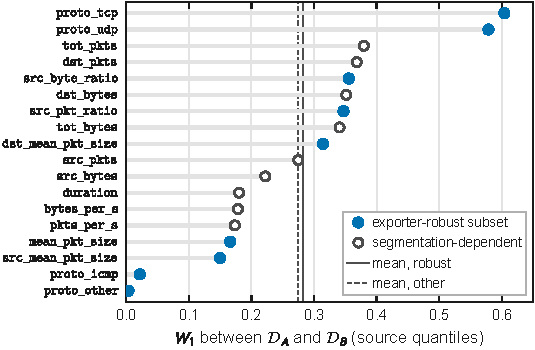
\includegraphics[width=\columnwidth]{../figures/generated/fig_rev_shift.pdf}
\caption{Covariate shift between \DA{} and \DB{} per shared column: first-order Wasserstein distance after the quantile transform fitted on source training data, Eq.~\eqref{eq:shift}. Filled markers are the exporter-robust subset, fixed before any result under it was computed; vertical lines are the two group means. The robust columns shift as much as the remaining columns, which indicates that the gap is not solely due to differences in how the two exporters segment flows.}
\label{fig:shift}
\DIFaddendFL \end{figure}

\DIFdelbegin \subsection{\DIFdel{On the Feature-Family Ablation}}
%DIFAUXCMD
\addtocounter{subsection}{-1}%DIFAUXCMD
%DIFDELCMD < \label{sec:ablation}
%DIFDELCMD < 
%%%
\DIFdelend \DIFaddbegin \begin{table}[t]
\caption{In-distribution cost of the shared space on \DA{} flows: all \NFullFeat{} non-port Zeek features against the 18 shared columns, same splits. Loss interval: Nadeau--Bengio corrected, 95\%.}
\label{tab:harm}
\centering
\scriptsize
\setlength{\tabcolsep}{2.6pt}
%DIF >  GENERATED by analysis/make_tables.py on 2026-09-26
%DIF >  source: EXP-052 harmonisation_loss (EXP-047, EXP-041)
%DIF >  commit: c19230c
%DIF >  DO NOT EDIT. Edit the generator, then re-run `make tables`.
\begin{tabular}{lccccc}
\toprule
Model & BA full & BA shared & Loss [95\% CI] & $F_1$ full & $F_1$ shared \\
\midrule
LR & 0.918 & 0.837 & +0.082 [-0.04, +0.20] & 0.725 & 0.626 \\
DT & 0.861 & 0.822 & +0.039 [-0.12, +0.20] & 0.663 & 0.619 \\
RF & 0.846 & 0.808 & +0.038 [-0.03, +0.11] & 0.726 & 0.701 \\
XGB & 0.885 & 0.864 & +0.020 [-0.05, +0.09] & 0.677 & 0.646 \\
HGB & 0.893 & 0.867 & +0.026 [-0.11, +0.16] & 0.680 & 0.647 \\
MLP & 0.917 & 0.912 & +0.005 [-0.08, +0.10] & 0.708 & 0.655 \\
\bottomrule
\end{tabular}

\DIFaddendFL 

\DIFdelbeginFL \DIFdelFL{An earlier version of this study reported a feature-family ablation and drew from it the claim that radio-layer telemetry, which contributes most to in-distribution accuracy }\DIFdelendFL \DIFaddbeginFL \end{table}

\subsection{\DIFadd{A Third Corpus}}
\label{sec:res:third}

\DIFadd{To test whether these results depend on the pair of corpora, we added }\DC{}\DIFadd{, the flow records of a 5G core testbed~\cite{nugraha2025fivegdatasets}, as a second target. It changes the site, the flow exporter, and the vantage point at once, and its labels, unlike those of }\DB{}\DIFadd{, are consistent. Only \ThConfShare\% of its flows lie on records that also occur with the opposite label}\DIFaddend , \DIFdelbegin \DIFdel{is also the primary source of deployment-specific overfitting, so that removing it improves transfer. }\DIFdelend \DIFaddbegin \DIFadd{and the upper bound on balanced accuracy in the shared columns is \ThCeilShared{}. When trained and tested on }\DC{} \DIFadd{itself, the six architectures achieve \ThRefShRandBAmin{} to \ThRefShRandBAmax{} on a random split and \ThRefShLofoBAmin{} to \ThRefShLofoBAmax{} when the capture file of one attack type is held out, so that this attack type is not seen during training.

}\DIFaddend 

\DIFdelbegin \DIFdel{\textbf{That claim is withdrawn.} It was registered in advance with a falsification condition, and the condition fired: the record-level join between the flow records and the radio telemetry cannot be established from the published artefacts, because the flow table carries no time column and shares no identifier with the radio layer. Without that join the ablation cannot be constructed at all, and no result we could report here would be supported by the data}\DIFdelend \DIFaddbegin \DIFadd{For transfer from }\DA{} \DIFadd{(Table~\ref{tab:third}, 20 split seeds), the balanced accuracy on }\DC{} \DIFadd{ranges from \ThATgtBAmin{} to \ThATgtBAmax{}, and ROC-AUC ranges from \ThATgtAUCmin{} to \ThATgtAUCmax. Every architecture detects the SYN flood, an attack type that is represented in training. Recall on the ICMP flood ranges from \ThAIcmpMin{} to \ThAIcmpMax{}, and recall on the control-plane PFCP attack ranges from \ThAPfcpMin{} to \ThAPfcpMax. The main source of error is the benign traffic of the new site. The false positive rate ranges from \ThAFPRmin{} to \ThAFPRmax{}, and up to \ThABgFlagMax{} of the signalling traffic of the core network is flagged. The loss relative to held-out source data, \ThADropMin{} to \ThADropMax{}, varies so much between split seeds that none is significant after correction. For transfer from }\DB{} \DIFadd{(10 split seeds), balanced accuracy spans \ThBTgtBAmin{} to \ThBTgtBAmax{}, and ROC-AUC is as low as \ThBTgtAUCmin{}. Which architecture transfers best depends on the pair of corpora, and no architecture transfers consistently. At $\pi = 0.002$, the highest operational precision at any threshold that retains recall above 10\% is \ThAPPVbest{} for transfer from }\DA{} \DIFadd{and \ThBPPVbest{} for transfer from }\DB{}\DIFadd{, and no architecture passes the deployability test in either direction (\ThAPredPass{} and \ThBPredPass{} of six). The pattern of Section~\ref{sec:res:transfer} recurs at a third site with a third exporter and consistent labels. The SYN flood is detected, and much of the site's benign traffic is not recognized as benign}\DIFaddend .

\DIFdelbegin \DIFdel{We record the withdrawal rather than deleting the question, because the question remains a good one andbecause the pre-registered failure criterion is what makes the withdrawal reportable rather than embarrassing. Fard \textit{et al.} publish the in-distribution half of the effect on this same corpus; the transfer half, which is the part that would have been ours, is untested. }\DIFdelend \DIFaddbegin \begin{table*}[t]
\caption{Transfer to the third corpus \DC{} (5G core testbed, NFStream flows~\cite{nugraha2025fivegdatasets}): balanced accuracy on held-out source data and on \DC{}, target ROC-AUC, recall per attack type, and the share of the core's background signalling flagged (Bkg.). Mean over 20 split seeds from \DA{} and 10 from \DB{}, at $\tau=0.5$.}
\label{tab:third}
\centering
\footnotesize
%DIF >  GENERATED by analysis/make_tables.py on 2026-09-26
%DIF >  source: EXP-052 third_* (EXP-058)
%DIF >  commit: c19230c
%DIF >  DO NOT EDIT. Edit the generator, then re-run `make tables`.
\begin{tabular}{lccccccccc}
\toprule
& \multicolumn{7}{c}{Trained on \DA{}} & \multicolumn{2}{c}{Trained on \DB{}} \\
Model & Src.\ BA & Tgt.\ BA & AUC & SYN & ICMP & PFCP & Bkg. & Tgt.\ BA & AUC \\
\midrule
LR & 0.837 & 0.742 & 0.800 & 1.00 & 0.10 & 0.00 & 0.27 & 0.517 & 0.726 \\
DT & 0.822 & 0.658 & 0.696 & 1.00 & 1.00 & 0.79 & 0.67 & 0.422 & 0.384 \\
RF & 0.808 & 0.596 & 0.926 & 1.00 & 1.00 & 0.99 & 0.81 & 0.540 & 0.697 \\
XGB & 0.864 & 0.640 & 0.888 & 1.00 & 1.00 & 0.74 & 0.70 & 0.688 & 0.814 \\
HGB & 0.867 & 0.698 & 0.932 & 1.00 & 1.00 & 0.80 & 0.61 & 0.565 & 0.632 \\
MLP & 0.912 & 0.691 & 0.837 & 1.00 & 0.20 & 0.61 & 0.44 & 0.848 & 0.766 \\
\textit{Maj.} & 0.500 & 0.500 & 0.500 & 1.00 & 1.00 & 1.00 & 1.00 & 0.500 & 0.500 \\
\bottomrule
\end{tabular}

\DIFaddendFL 

\DIFaddbeginFL \end{table*}
\DIFaddend \subsection{Alert Burden}
\DIFaddbegin \label{sec:res:alerts}

\DIFaddend 

\DIFdelbegin \DIFdel{Fig.~\ref{fig:alerts} sweeps the decision threshold and reports both the resulting hourly alert volume from \eqref{eq:alerts} and the operational precision from \eqref{eq:ppv}.

}%DIFDELCMD < 

%DIFDELCMD < %%%
\DIFdel{The gap between the two precision figures is }\DIFdelend \DIFaddbegin \DIFadd{Table~\ref{tab:pooled} reports pooled operating points at $\tau=0.5$ for three evaluation sets, together with 95\% cluster-bootstrap intervals. On the radio layer, }\DIFaddend the \DIFdelbegin \DIFdel{result. On the corpus, precision at }\DIFdelend \DIFaddbegin \DIFadd{six detectors have a pooled window-level false positive rate of \RadFPRmin{} to \RadFPRmax{} (\RadFAmin{} to \RadFAmax{} false alerts per benign UE-hour) and, at $\pi=0.002$, an operational precision of \RadPPVmin{} to \RadPPVmax{}, compared with a corpus precision of \RadPrecMin{} to \RadPrecMax{}. These point estimates are not stable. The false positive rate depends on which of the ten benign sessions are included in the test set (Table~\ref{tab:benign}), and the bootstrap interval of the pooled rate spans \RadCbFPRlo{} to \RadCbFPRhi{} across architectures, or \RadCbFAlo{} to \RadCbFAhi{} false alerts per benign UE-hour. Likewise, the interval for operational precision at }\DIFaddend $\tau=0.5$ \DIFdelbegin \DIFdel{is approximately }%DIFDELCMD < \measured{0.93} %%%
\DIFdel{for every detector, and the six are indistinguishable from one another. Translated through \eqref{eq:ppv} at $\pi=0.002$, pooled operational precision is between }%DIFDELCMD < \measured{0.0055} %%%
\DIFdel{and }%DIFDELCMD < \measured{0.0077} %%%
\DIFdel{--- a collapse by a factor of }%DIFDELCMD < \measured{132}%%%
\DIFdel{, with the detectors still indistinguishable. Alert volume runs to tens of thousands per hour, }\DIFdelend \DIFaddbegin \DIFadd{spans \RadCbPPVlo{} to \RadCbPPVhi{}. Thirty sessions cannot pin down the alert burden of the radio layer. They show only that it depends on }\DIFaddend the \DIFdelbegin \DIFdel{large majority false. }%DIFDELCMD < 

%DIFDELCMD < %%%
\DIFdel{Two properties of this collapse matter more than its size at any single operating point. First, it is not an artefact of the base rate we declared. Sweeping $\pi$ from }%DIFDELCMD < \measured{0.0001} %%%
\DIFdel{to }%DIFDELCMD < \measured{0.5} %%%
\DIFdel{moves the collapse factor from }%DIFDELCMD < \measured{2{,}631} %%%
\DIFdel{to }%DIFDELCMD < \measured{1.19}%%%
\DIFdel{, and the detectors remain within a factor of }%DIFDELCMD < \measured{1.40} %%%
\DIFdel{of one another throughout.Second, }\DIFdelend \DIFaddbegin \DIFadd{benign conditions a detector meets. On held-out }\DA{} \DIFadd{flows, }\DIFaddend the \DIFdelbegin \DIFdel{two-dimensional parameter space is really one-dimensional: operational precision depends on $\pi$ and is invariant to the benign arrival rate, while alert volume scales linearly in that rate and independently of it.
We verify both numerically rather than asserting them.

}\DIFdelend \DIFaddbegin \DIFadd{false positive rate is \NetSrcFPRmin{} to \NetSrcFPRmax{}, which at $\lambda_b = 240{,}000$ benign flows per hour corresponds to \NetSrcFAmin{} to \NetSrcFAmax{} false alerts per hour. On }\DB{}\DIFadd{, the false positive rate is \NetTgtFPRmin{} to \NetTgtFPRmax{}, or \NetTgtFAmin{} to \NetTgtFAmax{} false alerts per hour. Without the benign copies described in Section~\ref{sec:res:target}, it is \NetCleanFPRmin{} to \NetCleanFPRmax{}, which still amounts to \NetCleanFAmin{} to \NetCleanFAmax{} false alerts per hour, and the operational precision is \NetCleanPPVmin{} to \NetCleanPPVmax{}.

}\DIFaddend 

\DIFdelbegin \DIFdel{\textbf{A caution on how this quantity is estimated.} Operational precision is strongly non-linear }\DIFdelend \DIFaddbegin \DIFadd{Increasing the decision threshold improves precision only on held-out }\DA{} \DIFadd{flows (Fig.~\ref{fig:threshold}). The best threshold is chosen on the evaluation data, so the following values are upper bounds. With recall kept above 10\%, high thresholds reach an operational precision of \NetSrcPPVbest{} on held-out }\DA{} \DIFadd{flows, whereas the best value achieved by any detector on }\DB{} \DIFadd{is \NetTgtPPVbest{}, or \NetCleanPPVbest{} without the copies. On the radio layer, the best pooled value is \RadPPVbest{}, but its bootstrap interval reaches 1.0 for \RadCbBestHiN{} of the six architectures. A resample that omits the benign sessions flagged almost entirely leaves thresholds without any false positive. The relation between corpus precision and operational precision follows arithmetically from $\pi$. Varying $\pi$ from $10^{-4}$ to 0.5 changes the ratio between the two from \RadCollapseLowPi{} to \RadCollapseHighPi{} (Fig.~\ref{fig:prevalence}), so an operational precision is meaningful only when the assumed prevalence is stated.
\emph{Estimation of operational precision.} PPV is strongly nonlinear }\DIFaddend in the false positive rate near zero, so a \DIFdelbegin \DIFdel{single evaluation }\DIFdelend fold that happens to \DIFdelbegin \DIFdel{produce no false positives yields a precision of exactly one. Averaging that across folds, rather than pooling confusion counts, inflates the apparent spread between architectures: on our radio folds, which carry a median of }%DIFDELCMD < \measured{136} %%%
\DIFdel{benign windows, the same data gives a spread of }%DIFDELCMD < \measured{1.40} %%%
\DIFdel{pooledand }%DIFDELCMD < \measured{13.18} %%%
\DIFdelend \DIFaddbegin \DIFadd{contain no false positive yields $\mathrm{PPV}=1$ regardless of its recall. Averaging PPV over folds favors the architecture that happens to draw the most such folds. On the radio layer, the same counts yield a ratio between the best and the worst architecture of \EstPooled{} when pooled, \EstMedian{} as a median over folds, and \EstMean{} }\DIFaddend as a mean over folds \DIFdelbegin \DIFdel{. The distortion tracks the number of negatives per fold --- it is }%DIFDELCMD < \measured{1.4} %%%
\DIFdel{on the much larger network folds and vanishes when the target corpus is evaluated whole. We report }\DIFdelend \DIFaddbegin \DIFadd{(Table~\ref{tab:estimator}). We use }\DIFaddend pooled counts throughout\DIFdelbegin \DIFdel{, and report the mean alongside so that the size of the artefact remains visible. An earlier version of this work reported the mean. }\DIFdelend \DIFaddbegin \DIFadd{.

}\DIFaddend 

\DIFdelbegin \DIFdel{The cross-deployment case is considerably worse, and it separates the architectures in a way the source corpus does not. On }%DIFDELCMD < \DB{} %%%
\DIFdel{at $\tau=0.5$ the false positive rate ranges from }%DIFDELCMD < \measured{0.023} %%%
\DIFdel{for logistic regression to }%DIFDELCMD < \measured{0.885} %%%
\DIFdel{for the MLP. At the same benign flow rate that is }%DIFDELCMD < \measured{5{,}620} %%%
\DIFdel{false alerts per hour at one end and }%DIFDELCMD < \measured{212{,}383} %%%
\DIFdel{at the other, against pooled operational precisions of }%DIFDELCMD < \measured{0.0232} %%%
\DIFdel{and}%DIFDELCMD < \measured{0.0020} %%%
\DIFdel{respectively --- a factor of }%DIFDELCMD < \measured{23} %%%
\DIFdel{in burden for }%DIFDELCMD < \measured{0.042} %%%
\DIFdel{of }\DIFdelend \DIFaddbegin \begin{table*}[t]
\caption{Pooled operating points at $\tau=0.5$, 20 split seeds. FPR interval: 95\% cluster bootstrap resampling split seeds and clusters (radio sessions, \DA{} source addresses, \DB{} capture files; for flows from a deterministic re-run on 10 seeds, EXP-056, on which the ``w/o conflicts'' block is also computed). ``w/o conflicts'': \DB{} without the benign flows whose record also occurs with an attack label. PPV at $\pi=0.002$. $^{\dagger}$False alerts per benign UE-hour (radio, 225 windows per UE-hour) or per hour at $\lambda_b=240{,}000$ benign flows (flows). $^{\ddagger}$Highest pooled PPV over all thresholds with recall at least 0.10.}
\label{tab:pooled}
\centering
\footnotesize
%DIF >  GENERATED by analysis/make_tables.py on 2026-09-26
%DIF >  source: EXP-052 pooled_* and *_bootstrap (EXP-046, EXP-041, EXP-056)
%DIF >  commit: c19230c
%DIF >  DO NOT EDIT. Edit the generator, then re-run `make tables`.
\begin{tabular}{llcccccc}
\toprule
Corpus & Model & TPR & FPR [95\% CI] & Corpus $P$ & PPV & False alerts$^{\dagger}$ & Best PPV$^{\ddagger}$ \\
\midrule
\DA{} radio & LR & 0.798 & 0.223 [0.017, 0.547] & 0.921 & 0.0071 & 50 & 0.0130 \\
 & DT & 0.910 & 0.329 [0.086, 0.639] & 0.900 & 0.0055 & 74 & 0.0055 \\
 & RF & 0.954 & 0.267 [0.024, 0.650] & 0.921 & 0.0071 & 60 & 0.0360 \\
 & XGB & 0.931 & 0.251 [0.013, 0.606] & 0.924 & 0.0074 & 57 & 0.0116 \\
 & HGB & 0.945 & 0.262 [0.018, 0.615] & 0.922 & 0.0072 & 59 & 0.0086 \\
 & MLP & 0.895 & 0.222 [0.019, 0.560] & 0.929 & 0.0080 & 50 & 0.0109 \\
 & \textit{Maj.} & 1.000 & 1.000 [1.000, 1.000] & 0.766 & 0.0020 & 225 & 0.0020 \\
\midrule
\DA{} network & LR & 0.892 & 0.201 [0.126, 0.445] & 0.992 & 0.0088 & 48\,289 & 0.0297 \\
 & DT & 0.852 & 0.157 [0.068, 0.498] & 0.994 & 0.0108 & 37\,658 & 0.0120 \\
 & RF & 0.920 & 0.198 [0.121, 0.611] & 0.993 & 0.0092 & 47\,568 & 0.4172 \\
 & XGB & 0.884 & 0.090 [0.027, 0.373] & 0.997 & 0.0193 & 21\,625 & 0.2735 \\
 & HGB & 0.881 & 0.066 [0.031, 0.112] & 0.998 & 0.0262 & 15\,726 & 0.2727 \\
 & MLP & 0.905 & 0.071 [0.043, 0.349] & 0.997 & 0.0250 & 16\,996 & 0.2189 \\
 & \textit{Maj.} & 1.000 & 1.000 [1.000, 1.000] & 0.967 & 0.0020 & 240\,000 & 0.0020 \\
\midrule
\DB{} (transfer) & LR & 0.277 & 0.023 [0.009, 0.079] & 0.948 & 0.0232 & 5\,620 & 0.0258 \\
 & DT & 0.624 & 0.558 [0.111, 0.783] & 0.633 & 0.0022 & 133\,990 & 0.0022 \\
 & RF & 0.703 & 0.541 [0.121, 0.796] & 0.667 & 0.0026 & 129\,843 & 0.0027 \\
 & XGB & 0.552 & 0.429 [0.013, 0.687] & 0.666 & 0.0026 & 102\,890 & 0.0026 \\
 & HGB & 0.596 & 0.463 [0.031, 0.699] & 0.665 & 0.0026 & 111\,104 & 0.0026 \\
 & MLP & 0.646 & 0.539 [0.030, 0.745] & 0.649 & 0.0024 & 129\,320 & 0.0026 \\
 & \textit{Maj.} & 1.000 & 1.000 [1.000, 1.000] & 0.607 & 0.0020 & 240\,000 & 0.0020 \\
\midrule
\DB{} w/o conflicts & LR & 0.269 & 0.057 [0.038, 0.086] & 0.947 & 0.0094 & 13\,629 & 0.0102 \\
 & DT & 0.662 & 0.183 [0.103, 0.294] & 0.931 & 0.0072 & 44\,003 & 0.0077 \\
 & RF & 0.719 & 0.165 [0.118, 0.258] & 0.943 & 0.0087 & 39\,561 & 0.0629 \\
 & XGB & 0.531 & 0.026 [0.012, 0.047] & 0.987 & 0.0398 & 6\,158 & 0.0631 \\
 & HGB & 0.548 & 0.047 [0.030, 0.080] & 0.978 & 0.0227 & 11\,315 & 0.0587 \\
 & MLP & 0.612 & 0.053 [0.026, 0.102] & 0.977 & 0.0225 & 12\,794 & 0.0306 \\
 & \textit{Maj.} & 1.000 & 1.000 [1.000, 1.000] & 0.790 & 0.0020 & 240\,000 & 0.0020 \\
\bottomrule
\end{tabular}

\end{table*}

\begin{figure}[t]
\centering
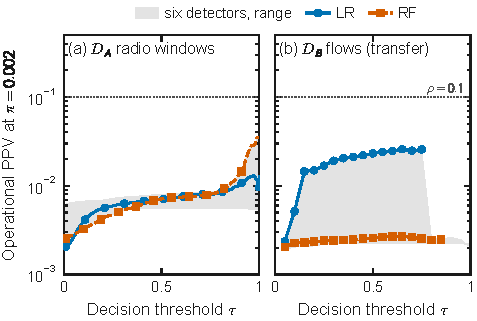
\includegraphics[width=\columnwidth]{../figures/generated/fig_rev_threshold.pdf}
\caption{Pooled operational precision at $\pi=0.002$ against the decision threshold on (a) the \DA{} radio layer and (b) \DB{} flows after transfer, at thresholds that keep recall at or above 0.10. The gray band spans the six architectures, and the dotted line marks the precision bound $\rho=0.1$ of the deployability test, which is not reached at any threshold on either evaluation set.}
\label{fig:threshold}
\end{figure}

\begin{figure}[t]
\centering
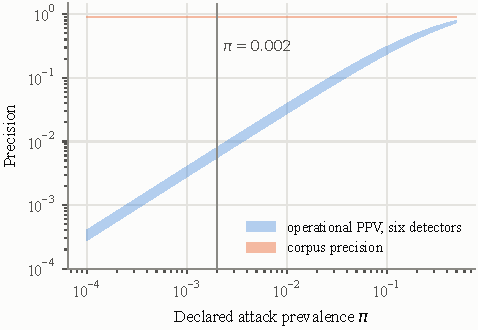
\includegraphics[width=\columnwidth]{../figures/generated/fig_rev_prevalence.pdf}
\caption{Pooled operational precision at $\tau=0.5$ against the declared attack prevalence $\pi$ for the six radio-layer detectors (one line each), with their corpus precision as a band. The dashed rule marks $\pi=0.002$. Operational precision is computed from the same confusion counts with Eq.~\eqref{eq:ppv}, and only the declared prevalence is varied.}
\label{fig:prevalence}
\end{figure}

\begin{table}[t]
\caption{Operational precision on the radio layer at $\tau=0.5$, $\pi=0.002$, estimated three ways from the same 20 folds.}
\label{tab:estimator}
\centering
\footnotesize
%DIF >  GENERATED by analysis/make_tables.py on 2026-09-26
%DIF >  source: EXP-052 estimator_contrast_radio (EXP-046)
%DIF >  commit: c19230c
%DIF >  DO NOT EDIT. Edit the generator, then re-run `make tables`.
\begin{tabular}{lcccc}
\toprule
Model & Folds with FP $=0$ & Pooled & Median & Mean \\
\midrule
LR & 1 & 0.0071 & 0.0118 & 0.0815 \\
DT & 0 & 0.0055 & 0.0070 & 0.0137 \\
RF & 1 & 0.0071 & 0.0092 & 0.0814 \\
XGB & 4 & 0.0074 & 0.0095 & 0.2185 \\
HGB & 2 & 0.0072 & 0.0091 & 0.1291 \\
MLP & 0 & 0.0080 & 0.0132 & 0.0476 \\
\bottomrule
\end{tabular}

\end{table}

\subsection{\DIFadd{Calibration and Prior Shift}}
\label{sec:res:calibration}

\DIFadd{Under transfer, the scores are poorly calibrated (Fig.~\ref{fig:reliability}). We fitted three calibrators on a group-disjoint calibration fold drawn from the source (Table~\ref{tab:calibration}). Whether a calibrator can alter the achievable operating points depends on whether it preserves the order of the scores. Temperature scaling preserves this order and changes ROC-AUC by at most \CalTempMax{}. Platt scaling is monotone, but its fitted slope can be negative, and for DT it inverted the ranking in \CalPlattFlipSeeds{} of \CalSeeds{} seeds, changing ROC-AUC by \CalPlattFlip. In that seed, the scores of the tree carried no ranking information on the calibration fold (ROC-AUC \PlattCalAUC{} on \PlattCalGroups{} held-out source addresses), although they ranked the test fold well (\PlattTestAUC). Platt scaling fitted the calibration fold correctly with a slope of \PlattSlope{} and, as a result, inverted the ranking on the test fold. The fault lies with small group-disjoint calibration folds, which need not resemble the test fold, and not with Platt scaling itself. Isotonic regression is monotone but piecewise constant, so it merges scores into ties and, on its fitting data, yields the ROC convex hull~\cite{fawcett2007pav}. Its largest change in ROC-AUC ranged from \CalIsoMin{} to \CalIsoMax{} across architectures. None of the calibrators raises the target }\DIFaddend macro-\DIFdelbegin \DIFdel{$F_{1}$. A transferred detector does not degrade gracefully into a noisier detector; it degrades into an alert generator that an operator will switch off within a shift }\DIFdelend \DIFaddbegin \DIFadd{$F_1$ above that of the raw scores for any architecture. Because they are fitted on a source containing \PrevDa\% attacks, they shift the scores toward that prior and flag more benign traffic on }\DB{}\DIFaddend .

\DIFdelbegin \DIFdel{Two points deserve emphasis because they run against the intuition the source corpus builds. First, }\DIFdelend \DIFaddbegin \DIFadd{The standard remedy for prior shift is to rescale the scores to the target prior~\cite{saerens2002adjusting}, which a deployment does not know. Expectation maximization~\cite{saerens2002adjusting} and black-box shift estimation~\cite{lipton2018bbse} estimate this prior from unlabeled data, assuming that only the class balance changes. Here that assumption fails. For a true target prior of \PriorTrue{}, the mean estimates per architecture range from \PriorMeanMin{} to \PriorMeanMax{}, and \PriorFracExtreme\% of }\DIFaddend the \DIFdelbegin \DIFdel{detectors are operationally \emph{indistinguishable} on held-out source data --- pooled PPV spans a factor of }%DIFDELCMD < \measured{1.40} %%%
\DIFdel{--- and an order of magnitude apart on the target, where the spread is }%DIFDELCMD < \measured{11.68}%%%
\DIFdel{. Which corpus one evaluates on decides whether the architectures look alike or not . Second, the model that wins }\DIFdelend \DIFaddbegin \DIFadd{individual estimates fall below 0.05 or above 0.95. Rescaling with the true prior, an oracle setting, does not beat the raw scores either (Table~\ref{tab:calibration}). What limits the detectors }\DIFaddend on the target \DIFdelbegin \DIFdel{operationally is the simplest one, and it is not the model that wins on macro-$F_{1}$ there.

Whichever single metric is chosen, it recommends a different system.

}\DIFdelend \DIFaddbegin \DIFadd{is discrimination (ROC-AUC \TrTgtAUCmin{} to \TrTgtAUCmax{}), not calibration.

}\DIFaddend 

\begin{figure}[t]
\centering
\DIFdelbeginFL %DIFDELCMD < \begin{tikzpicture}
%DIFDELCMD < \begin{axis}[
%DIFDELCMD <   scale only axis, width=0.62\columnwidth, height=4.2cm,
%DIFDELCMD <   axis y line*=left, axis x line*=bottom,
%DIFDELCMD <   ymode=log, ymin=25, ymax=1600,
%DIFDELCMD <   xmin=0.45, xmax=1.02,
%DIFDELCMD <   xlabel={Decision threshold $\tau$},
%DIFDELCMD <   ylabel={Alerts per hour},
%DIFDELCMD <   tick label style={font=\scriptsize}, label style={font=\scriptsize},
%DIFDELCMD <   ymajorgrids, grid style={dashed, gray!28}
%DIFDELCMD < ]
%DIFDELCMD < \addplot[thick, mark=*, mark size=1.6pt, color=blue!70!black]
%DIFDELCMD <   coordinates {(0.50,682) (0.70,463) (0.80,338) (0.90,211) (0.95,137) (0.99,46)};
%DIFDELCMD < \label{plt:alerts}
%DIFDELCMD < \end{axis}
%DIFDELCMD < \begin{axis}[
%DIFDELCMD <   scale only axis, width=0.62\columnwidth, height=4.2cm,
%DIFDELCMD <   axis y line*=right, axis x line=none,
%DIFDELCMD <   ymin=30, ymax=100,
%DIFDELCMD <   xmin=0.45, xmax=1.02,
%DIFDELCMD <   ylabel={Operational PPV / recall (\%)},
%DIFDELCMD <   tick label style={font=\scriptsize}, label style={font=\scriptsize},
%DIFDELCMD <   legend style={at={(0.02,0.03)}, anchor=south west, draw=none, font=\scriptsize, fill=white, fill opacity=0.85, text opacity=1}
%DIFDELCMD < ]
%DIFDELCMD < \addlegendimage{thick, mark=*, mark size=1.6pt, color=blue!70!black}\addlegendentry{alerts h$^{-1}$ (left)}
%DIFDELCMD < \addplot[thick, mark=square*, mark size=1.5pt, color=OliveGreen!75!black]
%DIFDELCMD <   coordinates {(0.50,41.2) (0.70,50.6) (0.80,58.4) (0.90,68.9) (0.95,75.6) (0.99,88.3)};
%DIFDELCMD < \addlegendentry{PPV at $\pi{=}0.002$}
%DIFDELCMD < \addplot[thick, dashed, mark=triangle*, mark size=1.8pt, color=red!70!black]
%DIFDELCMD <   coordinates {(0.50,99.21) (0.70,98.42) (0.80,97.55) (0.90,94.06) (0.95,88.31) (0.99,71.24)};
%DIFDELCMD < \addlegendentry{recall}
%DIFDELCMD < \end{axis}
%DIFDELCMD < \end{tikzpicture}
%DIFDELCMD < \caption{Alert burden and operational precision as the decision threshold varies, for XGBoost in distribution. The default threshold $\tau=0.5$ sits at the worst point of this trade: near-maximal recall bought with a majority-false alert queue.}
%DIFDELCMD < \label{fig:alerts}
%DIFDELCMD < %%%
\DIFdelendFL \DIFaddbeginFL 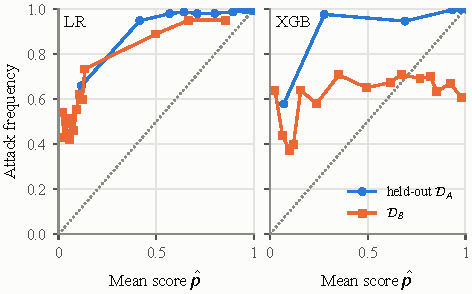
\includegraphics[width=\columnwidth]{../figures/generated/fig_rev_reliability.pdf}
\caption{Reliability diagrams for LR and XGB on held-out \DA{} and on \DB{}, fifteen equal-mass bins pooled over 20 split seeds.}
\label{fig:reliability}
\DIFaddendFL \end{figure}

\DIFdelbegin \subsection{\DIFdel{Latency and Resource Footprint}}

%DIFAUXCMD
\addtocounter{subsection}{-1}%DIFAUXCMD
\DIFdelend \DIFaddbegin \begin{table*}[t]
\caption{Calibration over 10 split seeds. Left: largest absolute change in ROC-AUC caused by each calibrator, over seeds and both evaluation sets. Right: target macro-$F_1$ at $\tau=0.5$ for raw scores, Platt and isotonic calibration, and Platt followed by prior correction with the EM estimate or the true (oracle) target prior.}
\label{tab:calibration}
\centering
\footnotesize
%DIF >  GENERATED by analysis/make_tables.py on 2026-09-26
%DIF >  source: EXP-044 calibration_runs
%DIF >  commit: c19230c
%DIF >  DO NOT EDIT. Edit the generator, then re-run `make tables`.
\begin{tabular}{lcccccccc}
\toprule
& \multicolumn{3}{c}{max $|\Delta$ROC-AUC$|$} & \multicolumn{5}{c}{Target macro-$F_1$ at $\tau=0.5$} \\
Model & Temp. & Platt & Iso. & Raw & Platt & Iso. & +EM & +Oracle \\
\midrule
LR & $<10^{-6}$ & $1\times10^{-6}$ & 0.209 & 0.538 & 0.415 & 0.391 & 0.327 & 0.478 \\
DT & $2\times10^{-5}$ & 0.946 & 0.170 & 0.538 & 0.395 & 0.405 & 0.447 & 0.436 \\
RF & $<10^{-6}$ & $<10^{-6}$ & 0.050 & 0.579 & 0.504 & 0.470 & 0.440 & 0.488 \\
XGB & $<10^{-6}$ & $<10^{-6}$ & 0.150 & 0.555 & 0.450 & 0.394 & 0.456 & 0.518 \\
HGB & $<10^{-6}$ & $<10^{-6}$ & 0.095 & 0.549 & 0.429 & 0.399 & 0.479 & 0.507 \\
MLP & $2\times10^{-5}$ & $2\times10^{-5}$ & 0.045 & 0.578 & 0.405 & 0.408 & 0.475 & 0.534 \\
\bottomrule
\end{tabular}

\DIFaddendFL 

\DIFaddbeginFL \end{table*}

\subsection{\DIFadd{Decision Latency}}
\label{sec:res:latency}

%DIF >  Results: decision latency (EXP-043). Numbers are macros from
%DIF >  tables/generated/numbers.tex, computed by analysis/latency_outputs.py.
\DIFaddend Table~\ref{tab:latency} reports the \DIFdelbegin \DIFdel{latency decomposition of \eqref{eq:latency} at an offered load of 1}%DIFDELCMD < {%%%
\DIFdel{,}%DIFDELCMD < }%%%
\DIFdel{000 decisions per second, together with sustainable throughput under the p99 constraint of \eqref{eq:budget} and container resource consumption. Fig.~\ref{fig:latency} shows how the }\DIFdelend \DIFaddbegin \DIFadd{per-call latency on one host for three implementations of each model. The first calls scikit-learn with a one-row pandas DataFrame, as our experiment code does. The second calls scikit-learn with a NumPy array on a single thread. The third uses ONNX Runtime on a single thread and is applied only where the exported model reproduces the decisions of scikit-learn (\LatOnnxOK{} of \LatOnnxN{} exports, with a decision agreement of at least \LatOnnxAgreeMin). A no-op call has a }\DIFaddend 99th \DIFdelbegin \DIFdel{percentile grows with load.

}%DIFDELCMD < 

%DIFDELCMD < %%%
\DIFdel{Three observations follow. First, median latency is a misleading summary. Four of the six architectures sit inside a 10}\DIFdelend \DIFaddbegin \DIFadd{percentile of \LatFloorPnn{}}\DIFaddend \,\DIFdelbegin \DIFdel{ms budget at $p_{50}$ and stay inside it at $p_{99}$; the two that do not --- histogram gradient boosting and the random forest --- miss it by an order of magnitude, with $p_{99}$ of }%DIFDELCMD < \measured{94.62} %%%
\DIFdel{and }%DIFDELCMD < \measured{378.05}%%%
\DIFdel{\,ms against medians of }%DIFDELCMD < \measured{53.16} %%%
\DIFdel{and }%DIFDELCMD < \measured{93.41}%%%
\DIFdel{\,}\DIFdelend ms\DIFdelbegin \DIFdel{. The tail, not the median, decides conformance}\DIFdelend \DIFaddbegin \DIFadd{, so platform overhead does not affect the comparisons}\DIFaddend .

\DIFdelbegin \DIFdel{Second, the verdict depends on where the budget is drawn, and O-RAN specifies the near-real-time loop over a range spanning two orders of magnitude. At 1}\DIFdelend \DIFaddbegin \DIFadd{The implementation has a larger effect on latency than the architecture (Fig.~\ref{fig:latency}). For LR, the DataFrame path takes \LatLRdfPfifty{}}\DIFaddend \,ms \DIFdelbegin \DIFdel{nothing conforms; at 5\,ms the decision tree alone; at 10\,ms the tree, logistic regression, XGBoost and }\DIFdelend \DIFaddbegin \DIFadd{at }\DIFaddend the \DIFdelbegin \DIFdel{MLP; at 100}\DIFdelend \DIFaddbegin \DIFadd{median against \LatLRarrPfifty{}}\DIFaddend \,ms \DIFdelbegin \DIFdel{all but the random forest; at 1}\DIFdelend \DIFaddbegin \DIFadd{for an array, and input validation accounts for the difference. For RF, predicting one row through the default thread pool takes \LatRFthreadsPfifty{}}\DIFaddend \,\DIFdelbegin \DIFdel{s everything. Asserting a single budget converts an authoring choice into an apparent measurement, so we report the crossing point per architecture instead.

}%DIFDELCMD < 

%DIFDELCMD < %%%
\DIFdel{Third, and least expected, inference is not the bottleneck. Packet-level feature extraction costs a median}%DIFDELCMD < \measured{6.90}%%%
\DIFdel{\,}\DIFdelend ms \DIFdelbegin \DIFdel{per flow against }%DIFDELCMD < \measured{0.18} %%%
\DIFdel{to }%DIFDELCMD < \measured{0.96}%%%
\DIFdelend \DIFaddbegin \DIFadd{at the median, compared with \LatRFarrPfifty{}}\DIFaddend \,ms \DIFdelbegin \DIFdel{of inference for the four architectureslight enough to meet a 10}\DIFdelend \DIFaddbegin \DIFadd{on one thread and \LatRFonnxPfifty{}}\DIFaddend \,ms \DIFdelbegin \DIFdel{budget. We re-implemented the exporter with bulk array extraction and measured a speed-up of }%DIFDELCMD < \measured{2.3} %%%
\DIFdel{to }%DIFDELCMD < \measured{12.1} %%%
\DIFdel{times, verified to produce identical flow records; extraction still costs }%DIFDELCMD < \measured{0.058}%%%
\DIFdelend \DIFaddbegin \DIFadd{in ONNX Runtime. Across architectures, the 99th percentile for ONNX Runtime lies between \LatOnnxPnnMin{} and \LatOnnxPnnMax{}}\DIFaddend \,ms \DIFdelbegin \DIFdel{per flow at best. Set against a deployed implementation rather than a prototype --- }%DIFDELCMD < \measured{1}%%%
\DIFdel{--}%DIFDELCMD < \measured{5}%%%
\DIFdelend \DIFaddbegin \DIFadd{on the radio layer, whereas it reaches up to \LatArrPnnMax{}}\DIFaddend \,\DIFdelbegin \DIFdel{$\mu$s }\DIFdelend \DIFaddbegin \DIFadd{ms }\DIFaddend for \DIFaddbegin \DIFadd{scikit-learn with arrays. Ranking architectures by latency largely ranks implementations, and a comparison with measurements from other hosts or languages~\cite{obiuwevwi2026realtime} says nothing about the architectures themselves. For context, Obiuwevwi et al. report inference times in the microsecond range for }\DIFaddend logistic regression \DIFdelbegin \DIFdel{inside a real Near-RT }\DIFdelend \DIFaddbegin \DIFadd{and a small MLP inside an OpenAirInterface and FlexRIC near-real-time }\DIFaddend RIC~\cite{obiuwevwi2026realtime}\DIFdelbegin \DIFdel{--- extraction is not merely the larger half of }\DIFdelend \DIFaddbegin \DIFadd{, within an order of magnitude of our ONNX Runtime figures.

}

\DIFadd{For a window-level detector, the decision path consists of window aggregation followed by inference. Aggregating one 16-record window requires \LatAggPnn{}\,ms at }\DIFaddend the \DIFdelbegin \DIFdel{budget but essentially the whole of it. Optimisation effort directed at model compression addresses the smaller part of the problem}\DIFdelend \DIFaddbegin \DIFadd{99th percentile}\DIFaddend , and the \DIFdelbegin \DIFdel{ranking of architectures by prototype latency is a statement about the prototype's toolchain rather than about the architectures }\DIFdelend \DIFaddbegin \DIFadd{upper bound of the 99th percentile of aggregation plus ONNX inference is at most \LatEtoEPnnHiMax{}\,ms across the architectures with a verified export. On this host, these two terms alone would meet any budget in the specified range. A repetition of the radio measurement on the same host, in which every call was recorded for Fig.~\ref{fig:latency}, yielded medians \LatRepMedRatioMin{} to \LatRepMedRatioMax{} times those in Table~\ref{tab:latency} (median ratio \LatRepMedRatio). Per-call latency on a host without CPU isolation thus depends on the state of the host as well as on the model. Nevertheless, the upper 95\% bound of the 99th percentile of aggregation plus ONNX inference remained at most \LatRepEtoEPnnHiMax\,ms in the repeated measurement}\DIFaddend .

%DIF <  WITHDRAWN (C15). An energy-per-decision comparison appeared here. RAPL reports
%DIF <  package and DRAM energy for a whole socket and cannot attribute it to a
%DIF <  container or a process, so the measurement the sentence described cannot be
%DIF <  made with the instrument it named. One row of one table is not worth an
%DIF <  indefensible claim. See configs/decisions.md and docs/claims.yaml C15.

\DIFaddbegin \DIFadd{Table~\ref{tab:ric} adds the remaining terms of Eq.~\eqref{eq:latency}, measured in the FlexRIC loop of Section~\ref{sec:setup}. We ran the six models with a report every 10\,ms (\RicNten{} reports each after 200 warm-up reports) and LR and RF with a report every 1\,ms (\RicNone{} reports each after 1,000 warm-up reports). A report carried \RicUEs{} UEs on average, and the xApp scored every one of them. At the 10\,ms period, a report needs \RicIndTenPfifty{}\,ms at the median to travel from the E2 node to the xApp, and the control round trip takes \RicActTenPfifty{}\,ms. Inference in the same loop takes at most \RicInfTenPnnMax{}\,ms at the 99th percentile. Delivery and control make up at least \RicTransportShareMin\% of the mean loop time for every model, so the choice of model has little effect once a RIC is in the path. The whole loop, from the report to the acknowledged control message, takes \RicLoopTenPnnMin{} to \RicLoopTenPnnMax{}\,ms at the 99th percentile, with an upper 95\% bound of at most \RicLoopTenPnnHiMax{}\,ms. It meets the smallest specified budget of 10\,ms at the 99.9th percentile as well (at most \RicLoopTenPnnnMax{}\,ms), and the largest single value at this period was \RicLoopTenMax{}\,ms.

}\DIFaddend 

%DIF <  [SYNTHETIC]
\DIFdelbegin %DIFDELCMD < \begin{table}[t]
%DIFDELCMD < \caption{Decision latency in milliseconds. \textbf{Measurement class: EMULATED} --- a Windows host, no CPU isolation, a single Python process, and no RIC in the path. These figures support relative ordering and stage decomposition; they support \emph{no} conformance claim. The no-op FLOOR runs first (D-007): its $p_{99}$ of \measured{0.103}\,ms is two orders of magnitude below the tightest budget, so nothing below it is a platform artefact. The final column is the smallest budget from the swept set $\{1,5,10,100,500,1000\}$\,ms at which the architecture's $p_{99}$ conforms.}
%DIFDELCMD < %%%
\DIFdelendFL \DIFaddbeginFL \DIFaddFL{The loop ran faster at the 1\,ms period. Its 99th percentile fell to \RicLoopOnePnnMin{} to \RicLoopOnePnnMax{}\,ms, the xApp never held more than \RicQueueMax{} reports in its queue, and no report was dropped in any run. Every term became faster, inference included (at most \RicInfOnePnnMax{}\,ms at the 99th percentile). We did not control CPU power management, and a host that idles between sparse reports and pays for waking up would produce this pattern. The loop runs on one host, with an emulated node and loopback SCTP. It therefore bounds the processing cost of the RIC software path, but it does not include the transport delay of a deployment.

}

\DIFaddFL{For a flow-level detector, feature construction is more costly than inference. On the three DDoS captures of }\DA{}\DIFaddFL{, the vectorized exporter produces flow records at \LatExtrMin{} to \LatExtrMax{}\,ms per flow, which is \LatExtrSpeedMin{} to \LatExtrSpeedMax{} times faster than the per-packet reference implementation on the same captures (\LatExtrRefMin{} to \LatExtrRefMax{}\,ms per flow), and the cost per flow increases with the number of packets per flow. On the \LatEqCaptures{} captures that were compared record by record, the two exporters agree exactly in packets and bytes on all \LatEqKeys{} shared IPv4 flow keys. The reference implementation additionally emits \LatRefOnlyMin{} and \LatRefOnlyMax{} IPv6 link-local keys, which the vectorized exporter does not parse because it supports IPv4 only. Mapping one exported record onto the shared space with the pandas code of our pipeline requires an additional \LatMapPfifty{}\,ms at the median, whereas ONNX inference on flow features requires at most \LatNetOnnxPnnMax{}\,ms at the 99th percentile. These figures describe a Python pipeline on a single host. They indicate that the cost lies mainly in feature construction, but they do not indicate what a native exporter at the user plane would cost.

}

\begin{table*}[t]
\caption{Per-call latency in milliseconds on one host (Section~\ref{sec:setup}): 20,000 calls after 1,000 warm-up calls, one thread per library, garbage collection enabled. No RIC in the path (Table~\ref{tab:ric} gives the loop through a RIC). Radio path $\overline{p}_{99}$: upper 95\% bound of the 99th percentile of window aggregation plus ONNX inference. Dashes: no export that reproduced scikit-learn's decisions.}
\DIFaddendFL \label{tab:latency}
\centering
\footnotesize
\DIFdelbeginFL %DIFDELCMD < \setlength{\tabcolsep}{4.5pt}
%DIFDELCMD < %%%
%DIF <  GENERATED by analysis/make_tables.py on 2026-09-21
%DIF <  source: results\EXP-005\processed\budget_sweep_radio.csv
%DIF <  commit: e45aa5b
\DIFdelendFL %DIF >  GENERATED by analysis/make_tables.py on 2026-09-26
%DIF >  source: EXP-043 latency_stages
%DIF >  commit: c19230c
% DO NOT EDIT. Edit the generator, then re-run `make tables`.
\DIFdelbeginFL %DIFDELCMD < \begin{tabular}{lccccc}
%DIFDELCMD < \toprule
%DIFDELCMD < Model & $p_{50}$ & $p_{95}$ & $p_{99}$ & $p_{99.9}$ & Min.\ budget \\
%DIFDELCMD < \midrule
%DIFDELCMD < FLOOR (no-op) & 0.01 & 0.02 & 0.10 & 0.53 & 1 \\
%DIFDELCMD < tree & 1.81 & 3.51 & 4.76 & 6.09 & 5 \\
%DIFDELCMD < logreg & 2.45 & 4.40 & 6.51 & 13.43 & 10 \\
%DIFDELCMD < xgboost & 3.83 & 6.19 & 7.29 & 11.39 & 10 \\
%DIFDELCMD < mlp & 2.25 & 4.95 & 8.17 & 13.98 & 10 \\
%DIFDELCMD < hgb & 53.16 & 74.76 & 94.62 & 446.06 & 100 \\
%DIFDELCMD < rf & 93.41 & 124.55 & 378.05 & 1034.91 & 500 \\
%DIFDELCMD < \bottomrule
%DIFDELCMD < \end{tabular}
%DIFDELCMD < 
%%%
\DIFdelendFL \DIFaddbeginFL \begin{tabular}{lccccccccc}
\toprule
& \multicolumn{2}{c}{sklearn, DataFrame} & \multicolumn{2}{c}{sklearn, array} & \multicolumn{2}{c}{ONNX Runtime} & Radio path & \multicolumn{2}{c}{Flow layer, $p_{99}$} \\
Model & $p_{50}$ & $p_{99}$ & $p_{50}$ & $p_{99}$ & $p_{50}$ & $p_{99}$ & $\overline{p}_{99}$ & array & ONNX \\
\midrule
LR & 0.44 & 0.72 & 0.11 & 0.17 & 0.010 & 0.023 & 0.12 & 0.16 & 0.025 \\
DT & 0.31 & 0.52 & 0.03 & 0.04 & 0.010 & 0.014 & 0.11 & 0.06 & 0.024 \\
RF & 6.25 & 12.99 & 5.57 & 21.50 & 0.012 & 0.024 & 0.10 & 4.45 & 0.029 \\
XGB & 0.73 & 1.00 & 0.16 & 0.32 & 0.011 & 0.021 & 0.09 & 0.40 & 0.024 \\
HGB & 1.48 & 2.72 & 1.17 & 1.92 & 0.013 & 0.035 & 0.12 & 1.22 & 0.034 \\
MLP & 0.43 & 0.67 & 0.11 & 0.21 & 0.017 & 0.035 & 0.11 & 0.15 & 0.037 \\
\bottomrule
\end{tabular}

\DIFaddendFL 

\DIFdelbeginFL %DIFDELCMD < \end{table}
%DIFDELCMD < 
%%%
\DIFdelend \DIFaddbegin \end{table*}

\DIFaddend 

\begin{figure}[t]
\centering
\DIFdelbeginFL %DIFDELCMD < 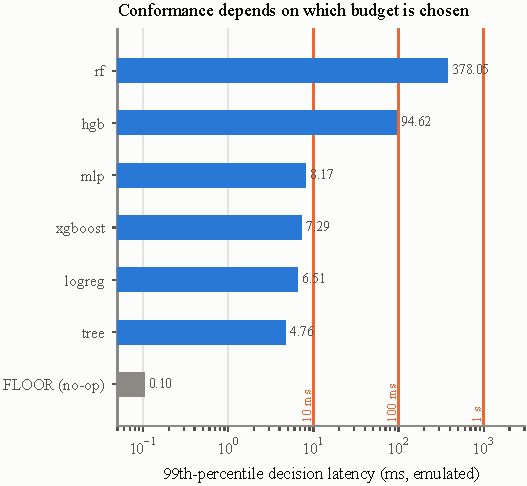
\includegraphics[width=\columnwidth]{../figures/generated/fig_latency_budget.pdf}
%DIFDELCMD < \caption{The conformance verdict is an authoring choice, not a measurement. O-RAN specifies the near-real-time loop over 10\,ms to 1\,s, and the same measurements support four different conclusions depending on where in that range the budget is drawn. Reporting the crossing point per architecture converts the choice back into a measurement. \textbf{Emulated}; see Table~\ref{tab:latency}.}
%DIFDELCMD < %%%
\DIFdelendFL \DIFaddbeginFL 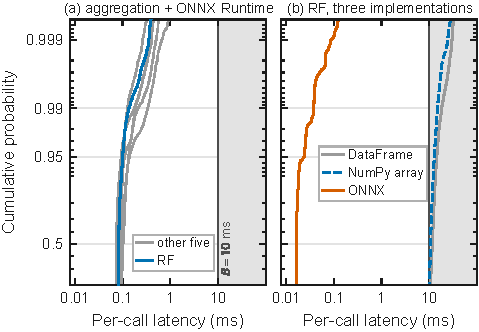
\includegraphics[width=\columnwidth]{../figures/generated/fig_rev_latency.pdf}
\caption{Empirical distribution of per-call latency for the radio layer on one host, 20,000 calls per stage, on a logit scale so that the median, 95th, and 99th percentiles are all visible. (a) The decision path of the deployability test, window aggregation followed by ONNX Runtime, for the six architectures. (b) One architecture, RF, under the three implementations of Table~\ref{tab:latency}. The shaded region lies beyond $B=10$\,ms, the smallest budget in the specified range. Only feature construction and inference are timed here. Table~\ref{tab:ric} gives the full loop through a RIC. The curves come from a repeat of the measurement that kept every call (EXP-060); Table~\ref{tab:latency} reports the original run.}
\DIFaddendFL \label{fig:latency}
\end{figure}

%DIF <  Measured results live in their own file so that real and synthetic numbers
%DIF <  cannot be confused while the draft banner is up. Everything it reports comes
%DIF <  from a generated table or figure; nothing in it was typed by hand.
%DIF <  =====================================================================
%DIF <   MEASURED RESULTS
%DIF < 
%DIF <   Everything in this file comes from a generated table under
%DIF <   tables/generated/ or a generated figure under figures/generated/.
%DIF <   No value here was typed by hand. Each \input has a provenance header
%DIF <   naming the result file and the git commit it was produced from.
%DIF < 
%DIF <   This file is kept separate from the synthetic body of main.tex on
%DIF <   purpose: while \synthdrafttrue is set, a reader must be able to tell
%DIF <   at a glance which numbers are real. Values here are wrapped in
%DIF <   \measured{} rather than \syn{}.
%DIF < 
%DIF <   Regenerate with:  make aggregate figures tables
%DIF <  =====================================================================
\DIFdelbegin %DIFDELCMD < 

%DIFDELCMD < %%%
\section{\DIFdel{Measured Results}}
%DIFAUXCMD
\addtocounter{section}{-1}%DIFAUXCMD
%DIFDELCMD < \label{sec:measured}
%DIFDELCMD < 

%DIFDELCMD < %%%
\DIFdel{This section reports measurements taken on the radio-telemetry layer of }%DIFDELCMD < \DA{} %%%
\DIFdel{under the run-disjoint protocol of Section~\ref{sec:setup}. Unless
stated otherwise every figure is a mean over }%DIFDELCMD < \measured{20} %%%
\DIFdel{split seeds, with intervals given as paired $t$-intervals over split means.Model
seeds are nested inside split seeds and averaged before testing, so the
effective sample size is the number of splits, not the number of fits. }%DIFDELCMD < 

%DIFDELCMD < %%%
\subsection{\DIFdel{Evaluation Protocol Effects}}
%DIFAUXCMD
\addtocounter{subsection}{-1}%DIFAUXCMD
%DIFDELCMD < \label{sec:measured:leakage}
%DIFDELCMD < 

%DIFDELCMD < %%%
\DIFdel{We first quantify how much of a reported score is attributable to the split protocol rather than to the detector. The same models, features and
seeds are evaluated twice: once under a random split over windows, the convention in much of the intrusion-detection literature, and once under a
split in which whole capture runs are held out.
}%DIFDELCMD < 

%DIFDELCMD < %%%
\DIFdelend \begin{table}[t]
\DIFdelbeginFL %DIFDELCMD < \caption{Effect of the split protocol on macro-$F_{1}$, \DA{} radio layer.
%DIFDELCMD < Differences are paired over \measured{20} split seeds; $^{\ast}$ marks
%DIFDELCMD < significance after Holm correction within the family of eight models.}
%DIFDELCMD < \label{tab:m_leakage}
%DIFDELCMD < %%%
\DIFdelendFL \DIFaddbeginFL \caption{Decision loop through a FlexRIC near-real-time RIC with an emulated E2 node on one host, in milliseconds, as ranges over models, at a reporting period of 10\,ms or 1\,ms. Terms follow Eq.~\eqref{eq:latency}: delivery from the E2 node to the xApp ($t_{\mathrm{ind}}$), queueing in the xApp ($t_{q}$), window aggregation ($t_{\mathrm{feat}}$) and ONNX Runtime inference ($t_{\mathrm{inf}}$) for one UE, and the control message up to its acknowledgment ($t_{\mathrm{act}}$). ``Loop'' runs from the timestamp in the KPM header to the acknowledgment, for the first UE of a report or for all its UEs.}
\label{tab:ric}
\DIFaddendFL \centering
%DIF <  GENERATED by analysis/make_tables.py on 2026-09-21
%DIF <  source: results\EXP-002\processed\leakage_summary.csv
%DIF <  commit: e45aa5b
\DIFaddbeginFL \scriptsize
\setlength{\tabcolsep}{2.4pt}
%DIF >  GENERATED by analysis/make_tables.py on 2026-09-26
%DIF >  source: EXP-061 ric_latency
%DIF >  commit: c19230c
\DIFaddendFL % DO NOT EDIT. Edit the generator, then re-run `make tables`.
\DIFdelbeginFL %DIFDELCMD < \begin{tabular}{lcccc}
%DIFDELCMD < \toprule
%DIFDELCMD < Model & Random & Run-disjoint & $\Delta$ & 95\,\% CI \\
%DIFDELCMD < \midrule
%DIFDELCMD < rf & 0.970 & 0.853 & +0.117$^{\ast}$ & [+0.057, +0.177] \\
%DIFDELCMD < mlp & 0.959 & 0.849 & +0.110$^{\ast}$ & [+0.056, +0.164] \\
%DIFDELCMD < hgb & 0.982 & 0.844 & +0.138$^{\ast}$ & [+0.082, +0.194] \\
%DIFDELCMD < xgboost & 0.977 & 0.837 & +0.140$^{\ast}$ & [+0.084, +0.195] \\
%DIFDELCMD < tree & 0.950 & 0.782 & +0.168$^{\ast}$ & [+0.110, +0.226] \\
%DIFDELCMD < logreg & 0.836 & 0.744 & +0.093$^{\ast}$ & [+0.037, +0.149] \\
%DIFDELCMD < stratified & 0.498 & 0.507 & -0.009$^{\ast}$ & [-0.011, -0.007] \\
%DIFDELCMD < majority & 0.431 & 0.434 & -0.002 & [-0.008, +0.003] \\
%DIFDELCMD < \bottomrule
%DIFDELCMD < \end{tabular}
%DIFDELCMD < %%%
\DIFdelendFL \DIFaddbeginFL \begin{tabular}{lcccc}
\toprule
& \multicolumn{2}{c}{10\,ms, six models} & \multicolumn{2}{c}{1\,ms, LR and RF} \\
Term & $p_{50}$ & $p_{99}$ & $p_{50}$ & $p_{99}$ \\
\midrule
$t_{\mathrm{ind}}$ & 1.51--1.86 & 3.02--3.05 & 0.51--0.53 & 0.84--0.98 \\
$t_{q}$ & 0.063--0.071 & 0.18--0.21 & 0.015--0.016 & 0.069 \\
$t_{\mathrm{feat}}$ & 0.001 & 0.002--0.003 & $<$0.001 & 0.001 \\
$t_{\mathrm{inf}}$ & 0.050--0.12 & 0.13--0.23 & 0.014--0.025 & 0.038--0.050 \\
$t_{\mathrm{act}}$ & 0.72--0.87 & 1.40--1.50 & 0.20--0.21 & 0.53--0.60 \\
\midrule
Loop, 1 UE & 2.38--2.97 & 4.36--4.59 & 0.76--0.79 & 1.38--1.59 \\
Loop, all & 2.48--3.18 & 4.45--4.95 & 0.77--0.86 & 1.42--1.69 \\
\bottomrule
\end{tabular}

\DIFaddendFL 

\end{table}

\DIFdelbegin %DIFDELCMD < 

%DIFDELCMD < %%%
\DIFdel{Table~\ref{tab:m_leakage} and Fig.~\ref{fig:m_leakage} show the result. Every
non-trivial architecture scores materially higher under the random split,
and all six differences survive Holm correction. The effect is not small:
it ranges from }%DIFDELCMD < \measured{9.3} %%%
\DIFdel{to }%DIFDELCMD < \measured{16.8} %%%
\DIFdel{points of macro-$F_{1}$,
with paired effect sizes $d_{z}$ between }%DIFDELCMD < \measured{0.78} %%%
\DIFdel{and }%DIFDELCMD < \measured{1.35}%%%
\DIFdel{.
}\DIFdelend 


\DIFdelbegin \DIFdel{Two features of the pattern matter more than its magnitude. First,the
ordering tracks model flexibility. A single depth-12 decision tree gains
most, the boosted ensembles next, the random forest and the multilayer
perceptron less, and logistic regression least. Second, the two trivial
baselines gain nothing: the majority-class classifier shows
$\Delta=\measured{-0.002}$ with $p=\measured{0.40}$. A classifier with no
capacity to memorise cannot profit from a leaky split, which is what
identifies the mechanism as memorisation rather than as a change in task
difficulty. }%DIFDELCMD < 

%DIFDELCMD < %%%
\DIFdel{The practical consequence is that the inflation cannot be treated as a
constant offset. It is largest for precisely the flexible architectures
that are most often reported, so a reader cannot mentally discount a
published random-split figure by a fixed amount.
}\DIFdelend \DIFaddbegin \section{\DIFadd{Discussion}}
\label{sec:discussion}

\DIFaddend 

\DIFdelbegin %DIFDELCMD < \begin{figure}[t]
%DIFDELCMD < \centering
%DIFDELCMD < 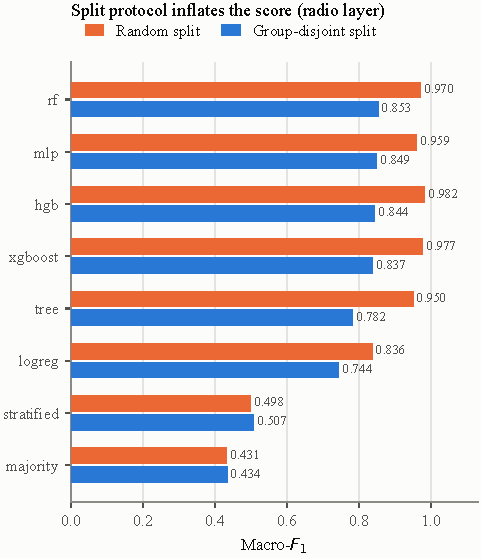
\includegraphics[width=\columnwidth]{../figures/generated/fig_leakage_radio.pdf}
%DIFDELCMD < \caption{Macro-$F_{1}$ under a random split and a run-disjoint split.
%DIFDELCMD < Bars are means over \measured{20} split seeds.}
%DIFDELCMD < \label{fig:m_leakage}
%DIFDELCMD < \end{figure}
%DIFDELCMD < %%%
\DIFdelend \DIFaddbegin \subsection{\DIFadd{Implications for O-RAN Practice}}
\label{sec:disc:practice}

\DIFaddend 

\DIFdelbegin \subsection{\DIFdel{Operational Alert Burden}}
%DIFAUXCMD
\addtocounter{subsection}{-1}%DIFAUXCMD
%DIFDELCMD < \label{sec:measured:alerts}
%DIFDELCMD < %%%
\DIFdelend \DIFaddbegin \DIFadd{\emph{Data path.} E2SM-KPM delivers aggregated measurements for each reporting period and does not carry packets. A window-level detector can operate inside the RIC on KPM reports, whereas a flow-level detector requires a flow exporter located near the user plane, either in the central unit or at the user-plane function, as well as a means of transporting its records to the xApp, for example through a custom E2 service model or the non-real-time data collection path. This transport adds to $t_{\mathrm{ind}}$ in Eq.~\eqref{eq:latency}. Our RIC loop measures $t_{\mathrm{ind}}$ for KPM reports only, so it does not cover the flow layer.

}\DIFaddend 

\DIFdelbegin \DIFdel{Criterion 2 asks what the detector costs an operator rather than how it
scores on a corpus. Table~\ref{tab:m_alerts} reports both quantities side by
side at the default threshold, under the declared deployment parameters
$\pi=0.002$ and $\lambda_{b}=240{,}000$ benign flows per hour}\DIFdelend \DIFaddbegin \DIFadd{\emph{Detection delay.} Computational latency accounts for only a small part of the total time to detection. A window-level decision cannot be made before the end of its window (16\,s in this study), and a flow-level decision cannot be made before the flow record is exported, which, for a long connection, requires an idle or active timeout to expire. The KPM reporting period and the flow timeouts should be reported together with the computational latency}\DIFaddend .

\DIFdelbegin %DIFDELCMD < \begin{table}[t]
%DIFDELCMD < \caption{Corpus precision against operational precision, \DA{} radio
%DIFDELCMD < layer, $\tau=0.5$. Both $\pi$ and $\lambda_{b}$ are declared deployment
%DIFDELCMD < parameters, not measurements; Fig.~\ref{fig:m_alerts} sweeps them.}
%DIFDELCMD < \label{tab:m_alerts}
%DIFDELCMD < \centering
%DIFDELCMD < %%%
%DIF <  GENERATED by analysis/make_tables.py on 2026-09-21
%DIF <  source: results\EXP-004\processed\alert_burden_radio.csv
%DIF <  commit: e45aa5b
%DIF <  DO NOT EDIT. Edit the generator, then re-run `make tables`.
%DIFDELCMD < \begin{tabular}{lcccccc}
%DIFDELCMD < \toprule
%DIFDELCMD < Model & Macro-$F_1$ & Corpus $P$ & Recall & FPR & Alerts/h & PPV \\
%DIFDELCMD < \midrule
%DIFDELCMD < rf & 0.852 & 0.926 & 0.954 & 0.262 & 63\,306 & 0.081 \\
%DIFDELCMD < mlp & 0.847 & 0.933 & 0.937 & 0.234 & 56\,571 & 0.036 \\
%DIFDELCMD < hgb & 0.844 & 0.928 & 0.945 & 0.257 & 62\,114 & 0.129 \\
%DIFDELCMD < xgboost & 0.838 & 0.930 & 0.931 & 0.247 & 59\,663 & 0.218 \\
%DIFDELCMD < logreg & 0.744 & 0.930 & 0.798 & 0.218 & 52\,638 & 0.081 \\
%DIFDELCMD < majority & 0.434 & 0.766 & 1.000 & 1.000 & 240\,481 & 0.002 \\
%DIFDELCMD < \bottomrule
%DIFDELCMD < \end{tabular}
%DIFDELCMD < 

%DIFDELCMD < \end{table}
%DIFDELCMD < 

%DIFDELCMD < %%%
\DIFdel{The two precision columns are the criterion in one line. Corpus precision
sits between }%DIFDELCMD < \measured{0.926} %%%
\DIFdel{and }%DIFDELCMD < \measured{0.933} %%%
\DIFdel{for all five detectors, a spread of }%DIFDELCMD < \measured{0.007}%%%
\DIFdel{. Once a realistic base rate is applied, the operational precision of the same five spans }%DIFDELCMD < \measured{0.036} %%%
\DIFdel{to
}%DIFDELCMD < \measured{0.218}%%%
\DIFdel{, a factor of six. The metric a paper would report cannot
distinguish these detectors; the metric an operator lives with separates
them sharply. Absolute volumes are }%DIFDELCMD < \measured{53{,}000} %%%
\DIFdel{to
}%DIFDELCMD < \measured{63{,}000} %%%
\DIFdel{alerts per hour, }\DIFdelend \DIFaddbegin \DIFadd{\emph{Acting on alerts.} An alert that triggers an E2SM-RC action, such as isolating or steering a UE, acts on a false alert in the same way as on a true one. At }\DIFaddend the \DIFdelbegin \DIFdel{large majority of them false. }\DIFdelend \DIFaddbegin \DIFadd{false positive rates reported in Table~\ref{tab:pooled}, automatic mitigation on the radio layer would act against each benign UE \RadFAmin{} to \RadFAmax{} times per hour. Alerts of this quality may inform an operator or a non-real-time policy through A1, but they should not trigger automatic control actions.

}\DIFaddend 

\DIFdelbegin \DIFdel{None of this is a new statistical result. The base-rate argument is
Axelsson's, and it is a quarter of a century old.

What is new is its
quantification for a specific detectorunder a protocol that holds capture
runs out, reported alongside the tail-latency measurement for the same
model artefacts. }%DIFDELCMD < 

%DIFDELCMD < %%%
\DIFdel{A second and less expected finding concerns the operator's only runtime
control. Sweeping the decision threshold to recover precision, Table~\ref{tab:m_ppvcross} shows that $\text{PPV}=0.5$ is \emph{unreachable at any threshold} for four of the five detectors. The
scores of the boosted models and the perceptron saturate near unity under
a run-disjoint split, so raising $\tau$ barely moves the alert volume: the
histogram-boosted ensemble still emits }%DIFDELCMD < \measured{53{,}632} %%%
\DIFdel{alerts per hour
at $\tau=\measured{0.99}$. Only the random forest and the linear model
reach $\text{PPV}=0.5$, and both do so by collapsing recall, to
}%DIFDELCMD < \measured{0.418} %%%
\DIFdel{and }%DIFDELCMD < \measured{0.189} %%%
\DIFdel{respectively. This is a calibration
failure with an immediate operational consequence, and it is invisible in accuracy, $F_{1}$ or AUC}\DIFdelend \DIFaddbegin \DIFadd{\emph{Admission and monitoring.} The deployability test of Eq.~\eqref{eq:deploy} can serve as an admission check before an xApp is enabled at a new site, provided that labeled benign and attack traffic is available from that site. After admission, unsupervised shift detection~\cite{rabanser2019failing} can indicate when the incoming traffic departs from the training distribution. Because the corpora studied here can be distinguished with a balanced accuracy of \DomShared{}, such a monitor would raise an alarm immediately}\DIFaddend .

\DIFdelbegin %DIFDELCMD < \begin{table}[t]
%DIFDELCMD < \caption{Decision threshold required to reach a usable operational
%DIFDELCMD < precision, and its cost in recall and alert volume.}
%DIFDELCMD < \label{tab:m_ppvcross}
%DIFDELCMD < \centering
%DIFDELCMD < %%%
%DIF <  GENERATED by analysis/make_tables.py on 2026-09-21
%DIF <  source: results\EXP-004\processed\ppv_crossings_radio.csv
%DIF <  commit: e45aa5b
%DIF <  DO NOT EDIT. Edit the generator, then re-run `make tables`.
%DIFDELCMD < \begin{tabular}{lcccc}
%DIFDELCMD < \toprule
%DIFDELCMD < Model & PPV target & $\tau$ required & Recall & Alerts/h \\
%DIFDELCMD < \midrule
%DIFDELCMD < rf & 0.10 & 0.55 & 0.945 & 60\,768 \\
%DIFDELCMD < rf & 0.25 & 0.65 & 0.921 & 57\,251 \\
%DIFDELCMD < rf & 0.50 & 0.95 & 0.418 & 7\,521 \\
%DIFDELCMD < mlp & 0.10 & 0.60 & 0.922 & 52\,993 \\
%DIFDELCMD < mlp & 0.25 & 0.85 & 0.852 & 44\,500 \\
%DIFDELCMD < mlp & 0.50 & \textit{unreachable} & -- & -- \\
%DIFDELCMD < hgb & 0.10 & 0.40 & 0.948 & 62\,706 \\
%DIFDELCMD < hgb & 0.25 & 0.99 & 0.898 & 53\,632 \\
%DIFDELCMD < hgb & 0.50 & \textit{unreachable} & -- & -- \\
%DIFDELCMD < xgboost & 0.10 & 0.20 & 0.957 & 65\,758 \\
%DIFDELCMD < xgboost & 0.25 & 0.55 & 0.926 & 59\,036 \\
%DIFDELCMD < xgboost & 0.50 & \textit{unreachable} & -- & -- \\
%DIFDELCMD < logreg & 0.10 & 0.65 & 0.715 & 43\,305 \\
%DIFDELCMD < logreg & 0.25 & 0.85 & 0.514 & 26\,981 \\
%DIFDELCMD < logreg & 0.50 & 0.99 & 0.189 & 8\,855 \\
%DIFDELCMD < majority & 0.10 & \textit{unreachable} & -- & -- \\
%DIFDELCMD < majority & 0.25 & \textit{unreachable} & -- & -- \\
%DIFDELCMD < majority & 0.50 & \textit{unreachable} & -- & -- \\
%DIFDELCMD < \bottomrule
%DIFDELCMD < \end{tabular}
%DIFDELCMD < %%%
\DIFdelendFL \DIFaddbeginFL \subsection{\DIFaddFL{Applying the Deployability Test}}
\label{sec:disc:predicate}

\DIFaddendFL 

\DIFdelbeginFL %DIFDELCMD < \end{table}
%DIFDELCMD < 

%DIFDELCMD < \begin{figure*}[t]
%DIFDELCMD < \centering
%DIFDELCMD < 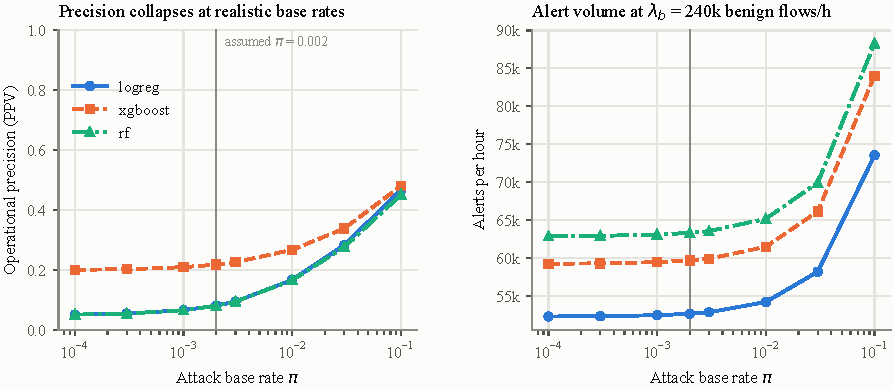
\includegraphics[width=\textwidth]{../figures/generated/fig_alert_burden.pdf}
%DIFDELCMD < \caption{Operational precision and alert volume against the attack base
%DIFDELCMD < rate $\pi$. Both panels share one vertical scale each; the vertical rule
%DIFDELCMD < marks the $\pi$ assumed in Table~\ref{tab:m_alerts}.}
%DIFDELCMD < \label{fig:m_alerts}
%DIFDELCMD < \end{figure*}
%DIFDELCMD < 

%DIFDELCMD < %%%
\subsection{\DIFdel{Decision Latency Against a Swept Budget}}
%DIFAUXCMD
\addtocounter{subsection}{-1}%DIFAUXCMD
%DIFDELCMD < \label{sec:measured:latency}
%DIFDELCMD < 

%DIFDELCMD < \begin{table}[t]
%DIFDELCMD < \caption{Per-decision latency, \DA{} radio layer, \measured{1500}
%DIFDELCMD < repetitions after warm-up. The last column gives the smallest near-real-time
%DIFDELCMD < budget each architecture's 99th percentile conforms to.
%DIFDELCMD < \textbf{These are emulated measurements}; see Section~\ref{sec:limitations}.}
%DIFDELCMD < \label{tab:m_latency}
%DIFDELCMD < \centering
%DIFDELCMD < %%%
%DIF <  GENERATED by analysis/make_tables.py on 2026-09-21
%DIF <  source: results\EXP-005\processed\budget_sweep_radio.csv
%DIF <  commit: e45aa5b
%DIF <  DO NOT EDIT. Edit the generator, then re-run `make tables`.
%DIFDELCMD < \begin{tabular}{lccccc}
%DIFDELCMD < \toprule
%DIFDELCMD < Model & $p_{50}$ & $p_{95}$ & $p_{99}$ & $p_{99.9}$ & Min.\ budget \\
%DIFDELCMD < \midrule
%DIFDELCMD < FLOOR (no-op) & 0.01 & 0.02 & 0.10 & 0.53 & 1 \\
%DIFDELCMD < tree & 1.81 & 3.51 & 4.76 & 6.09 & 5 \\
%DIFDELCMD < logreg & 2.45 & 4.40 & 6.51 & 13.43 & 10 \\
%DIFDELCMD < xgboost & 3.83 & 6.19 & 7.29 & 11.39 & 10 \\
%DIFDELCMD < mlp & 2.25 & 4.95 & 8.17 & 13.98 & 10 \\
%DIFDELCMD < hgb & 53.16 & 74.76 & 94.62 & 446.06 & 100 \\
%DIFDELCMD < rf & 93.41 & 124.55 & 378.05 & 1034.91 & 500 \\
%DIFDELCMD < \bottomrule
%DIFDELCMD < \end{tabular}
%DIFDELCMD < 

%DIFDELCMD < \end{table}
%DIFDELCMD < 

%DIFDELCMD < %%%
\DIFdelend %DIF >  Discussion: applying the deployability test of Eq. (7). Numbers are macros
%DIF >  from tables/generated/numbers.tex; the table is generated (EXP-052).
\DIFaddbegin \DIFadd{We instantiate Eq.~\eqref{eq:deploy} with the bounds described below. These bounds were chosen by us, since no }\DIFaddend O-RAN \DIFdelbegin \DIFdel{specifies the near-real-time control loop over a range of }\DIFdelend \DIFaddbegin \DIFadd{specification defines them, and an operator would set them according to its own traffic and staffing. The generalization bound is $\delta = 0.10$ in balanced accuracy and is applied to the upper end of the corrected 95\% interval. The alert term requires a threshold that detects at least half of the attacks ($r_{\min} = 0.5$), for which at least one alert in ten is a true alert ($\rho = 0.1$ at $\pi = 0.002$), and which raises at most $A_{\max} = 200$ false alerts per hour at $\lambda_{b} = 240{,}000$ benign flows per hour. All alert conditions are evaluated on }\DB{}\DIFadd{, because a detector is deployed on the target rather than on the source. The latency term uses the strictest budget permitted by the specification, $B = 10$\,ms. We evaluate it on the FlexRIC loop at a }\DIFaddend 10\,\DIFdelbegin \DIFdel{ms to
1\,s rather than at a single value. Reporting conformance against one
chosen point inside that range makes the verdict an artefact of the
choice. Table~\ref{tab:m_latency} and Fig.~\ref{fig:m_latency} therefore report,
for each architecture, the smallest budget its }\DIFdelend \DIFaddbegin \DIFadd{ms reporting period. There the upper bound of the }\DIFaddend 99th \DIFdelbegin \DIFdel{percentile conforms to.
}%DIFDELCMD < 

%DIFDELCMD < %%%
\DIFdel{The floor experiment was run first. A no-op model on the same path yields
$p_{99}=\measured{0.103}$}\DIFdelend \DIFaddbegin \DIFadd{percentile is at most \RicLoopTenPnnHiMax{}}\DIFaddend \,\DIFdelbegin \DIFdel{ms, two orders of magnitude below the tightest
budget considered, so the ordering below is a property of the models rather
than of the measurement platform.
}%DIFDELCMD < 

%DIFDELCMD < %%%
\DIFdel{The verdict moves with the budget. At }%DIFDELCMD < \measured{1}%%%
\DIFdel{\,ms no architecture
conforms. At }%DIFDELCMD < \measured{5}%%%
\DIFdel{\,ms only the single decision tree does. At
}%DIFDELCMD < \measured{10}%%%
\DIFdel{\,ms four of six conform.

At }%DIFDELCMD < \measured{1000}%%%
\DIFdel{\,ms all of them
do.One set of measurements thus supports four different conclusions,
separated only by where the line is drawn, which is }\DIFdelend \DIFaddbegin \DIFadd{ms for every architecture (Section~\ref{sec:res:latency}), so the term is satisfied for any budget in the specified range, on one host and with an emulated E2 node.

}

\DIFadd{Table~\ref{tab:predicate} presents the result, according to which none of the architectures passes the test (\PredPass{} of six). Every architecture fails the generalization term, with upper bounds of \PredGenMin{} to \PredGenMax{}, and every architecture also fails the alert term by a wide margin. At a recall of at least 0.5, the highest operational precision on }\DB{} \DIFadd{is \PredPPVmax{}, and the smallest number of false alerts per hour is \PredFAmin{}. The verdict is therefore robust to the choice of bounds. It holds for any $\rho$ above \PredPPVmax{}, any $A_{\max}$ below \PredFAmin{} per hour, and any $\delta$ below \PredGenMin{}, and it does not depend on the latency term. Nor does it depend on the declared prevalence. The number of false alerts does not involve $\pi$ and exceeds $A_{\max}$ at every threshold, and the precision condition alone would require $\pi \ge \PredPiStar$, which is \PredPiStarRatio{} times the declared value. The verdict is also unaffected by the label conflicts described in Section~\ref{sec:res:target}. When the test is evaluated on }\DB{} \DIFadd{without the benign copies, \PredCleanPass{} of six architectures pass, the highest operational precision at a recall of at least 0.5 is \PredCleanPPVmax{}, and }\DIFaddend the \DIFdelbegin \DIFdel{reason to report
the crossing point instead of }\DIFdelend \DIFaddbegin \DIFadd{smallest number of false alerts per hour is \PredCleanFAmin. On these flows the precision condition alone would hold from $\pi = \PredCleanPiStar$, but the number of false alerts still excludes every architecture. Fig.~\ref{fig:sensitivity} shows how far the bounds would have to be relaxed. An architecture satisfies the alert term only if an operator accepts several thousand false alerts per hour and }\DIFaddend a \DIFdelbegin \DIFdel{pass-fail column.
}\DIFdelend \DIFaddbegin \DIFadd{precision of a few percent, and it satisfies the generalization term only if $\delta$ exceeds \PredGenMin{}. The latency term would matter only if the first two were satisfied, and in our loop it is met with a margin of about a factor of two at the smallest specified budget.

}\DIFaddend 

\DIFaddbegin \begin{table}[t]
\caption{Deployability test of Eq.~\eqref{eq:deploy} per architecture. $\overline{\Delta}_{\mathrm{BA}}$: upper 95\% bound of the balanced-accuracy loss (pass if $\le 0.10$). Best PPV and minimum false alerts per hour over thresholds with recall $\ge 0.5$ on \DB{} (pass if PPV $\ge 0.1$ and alerts $\le 200$). $B_{\min}$: smallest budget of the series 1, 2, 5, 10\,ms met by the upper 95\% bound of the 99th percentile of the FlexRIC loop (all UEs of a report, 10\,ms period, emulated E2 node).}
\label{tab:predicate}
\centering
\scriptsize
\setlength{\tabcolsep}{2.4pt}
%DIF >  GENERATED by analysis/make_tables.py on 2026-09-26
%DIF >  source: EXP-052 predicate (EXP-041, EXP-061)
%DIF >  commit: c19230c
%DIF >  DO NOT EDIT. Edit the generator, then re-run `make tables`.
\begin{tabular}{lccccccc}
\toprule
Model & $\overline{\Delta}_{\mathrm{BA}}$ & Gen. & Best PPV & Min.\ alerts/h & Alert & $B_{\min}$ (ms) & $\mathcal{P}$ \\
\midrule
LR & 0.32 & $\times$ & 0.0024 & 166\,328 & $\times$ & 5 & 0 \\
DT & 0.50 & $\times$ & 0.0022 & 118\,342 & $\times$ & 5 & 0 \\
RF & 0.47 & $\times$ & 0.0027 & 98\,410 & $\times$ & 5 & 0 \\
XGB & 0.47 & $\times$ & 0.0026 & 95\,507 & $\times$ & 5 & 0 \\
HGB & 0.47 & $\times$ & 0.0026 & 99\,277 & $\times$ & 10 & 0 \\
MLP & 0.50 & $\times$ & 0.0026 & 105\,744 & $\times$ & 5 & 0 \\
\bottomrule
\end{tabular}

\end{table}

\DIFaddend \begin{figure}[t]
\centering
\DIFdelbeginFL %DIFDELCMD < 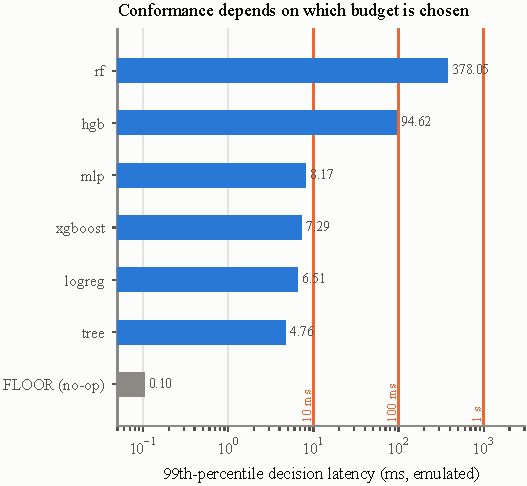
\includegraphics[width=\columnwidth]{../figures/generated/fig_latency_budget.pdf}
%DIFDELCMD < \caption{99th-percentile decision latency per architecture. Vertical rules
%DIFDELCMD < mark three points inside the specified near-real-time range.}
%DIFDELCMD < \label{fig:m_latency}
%DIFDELCMD < %%%
\DIFdelendFL \DIFaddbeginFL 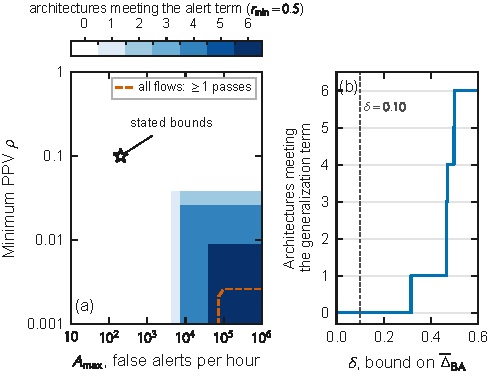
\includegraphics[width=\columnwidth]{../figures/generated/fig_rev_sensitivity.pdf}
\caption{Sensitivity of the deployability test to its bounds. (a) Number of the six architectures meeting the alert term ($r_{\min}=0.5$, $\pi=0.002$, $\lambda_b=240{,}000$ flows per hour) on \DB{} without the benign copies, as the alert bound $A_{\max}$ and the precision bound $\rho$ vary; on all flows, at least one architecture passes only below and to the right of the dashed line. The star marks the bounds we use. (b) Number of architectures meeting the generalization term as $\delta$ varies. A detector passes the test only if both terms are satisfied.}
\label{fig:sensitivity}
\DIFaddendFL \end{figure}

\DIFdelbegin \DIFdel{Decomposing the path shows where the time goes.Model inference accounts
for }%DIFDELCMD < \measured{0.18} %%%
\DIFdel{to }%DIFDELCMD < \measured{0.96}%%%
\DIFdel{\,ms for the four architectures that
conform at 10\,ms, whereas constructing features from packets costs a
median }%DIFDELCMD < \measured{6.90}%%%
\DIFdel{\,ms per flow, ranging from }%DIFDELCMD < \measured{4.49} %%%
\DIFdel{to }%DIFDELCMD < \measured{37.34}%%%
\DIFdel{\,ms across captures. For those architectures feature
construction is between }%DIFDELCMD < \measured{7} %%%
\DIFdel{and }%DIFDELCMD < \measured{39} %%%
\DIFdel{times the cost of inference. The relation inverts for the random forest and the
histogram-boosted ensemble, whose own inference exceeds extraction, so the
observation is architecture-dependent and is stated as such.
}%DIFDELCMD < 

%DIFDELCMD < %%%
\DIFdel{Two caveats bound this. The exporter is a reference implementation in
Python running at }%DIFDELCMD < \measured{1.1} %%%
\DIFdel{to }%DIFDELCMD < \measured{4.3}%%%
\DIFdel{\,MB/s, and }\DIFdelend \DIFaddbegin \DIFadd{\emph{Attainability of the test.} A test that no detector passes might simply be too strict. The published 5G-NIDD pipeline described in Section~\ref{sec:res:target} indicates that this is not the case. On its own random split, with the alert term evaluated on that split, \PubRzPassN{} of its five classifiers pass the test, with an operational precision of up to \PubRzPPVmax{} at $\pi = 0.002$ and as few as \PubRzFAmin{} false alerts per hour at $\lambda_b = 240{,}000$. The same pipeline fails the test at the next rung, when the two position counters are removed, and at every subsequent rung, both on all flows and on the flows without the benign copies (Table~\ref{tab:ladder}). The informativeness of the test is therefore limited by the evaluation to which it is applied. When applied to }\DIFaddend a \DIFdelbegin \DIFdel{native
implementation would be substantially faster; the defensible claim is therefore that feature construction is of the same order as or larger than inference for every architecture that meets a 10\,ms budget, so optimising
the model alone addresses the smaller part of the budget. Per-flow cost
also varies roughly eightfold across captures because it is driven by
packets per flow rather than by flow count, which is why the range is reported beside the median.

}\DIFdelend \DIFaddbegin \DIFadd{random split that still contains record positions, it merely confirms the result of that split, and the pass disappears as soon as the evaluation moves one step closer to deployment conditions. The detectors examined in this paper fail the test under the evaluations closest to deployment that the available corpora permit.

}\DIFaddend 


\DIFdelbegin \section{\DIFdel{Comparative Analysis}}
%DIFAUXCMD
\addtocounter{section}{-1}%DIFAUXCMD
%DIFDELCMD < \label{sec:comparative}
%DIFDELCMD < 
%%%
\DIFdelend \DIFaddbegin \subsection{\DIFadd{Relation to Reported Results}}

\DIFaddend 

\DIFdelbegin \subsection{\DIFdel{Against the Reported State of the Art}}

%DIFAUXCMD
\addtocounter{subsection}{-1}%DIFAUXCMD
%DIFDELCMD < 

%DIFDELCMD < %%%
\DIFdel{Direct numerical comparison with published }\DIFdelend \DIFaddbegin \DIFadd{Most published results for }\DIFaddend O-RAN \DIFdelbegin \DIFdel{intrusion detection results is not meaningful, because those results are }\DIFdelend \DIFaddbegin \DIFadd{and 5G intrusion detection are }\DIFaddend in-distribution \DIFdelbegin \DIFdel{scores on corpora we do not share, and }\DIFdelend \DIFaddbegin \DIFadd{scores obtained on corpora that differ from ours, and }\DIFaddend our own in-distribution \DIFdelbegin \DIFdel{scores in Table~\ref{tab:indist} are in the same range. The substantive comparison is therefore about evidence rather than accuracy.

}%DIFDELCMD < 

%DIFDELCMD < %%%
\DIFdel{We surveyed reporting practice using the following protocol. We queried IEEE Xplore, the ACM Digital Library and Scopus for records published between January 2021 and December 2025 matching (\texttt{"O-RAN" OR "Open RAN" OR "5G"})\texttt{AND} (\texttt{"intrusion detection" OR "anomaly detection"}) \texttt{AND} (\texttt{"machine learning" OR "deep learning"}), restricted to peer-reviewed conference and journal papers in English. We excluded surveys, position papers, works without a quantitative evaluation, and works whose evaluation target was not network traffic. Two authors screened titles and abstracts independently and resolved disagreements by discussion, then assessed the full text of retained records against the eight reporting properties of Table~\ref{tab:survey}. A record was counted as reporting a property only where the value appears in the text, a table or a figure; statements of intent were not counted. Table~\ref{tab:survey} gives the resulting counts. Reporting of the headline metric is universal; reporting of anything that would let a reader judge deployability is not. }%DIFDELCMD < 

%DIFDELCMD < %%%
%DIF <  [SYNTHETIC] --- counts are placeholders. The protocol below is real and
%DIF <  executable; run it and substitute the resulting counts before submission.
%DIFDELCMD < \begin{table}[t]
%DIFDELCMD < \caption{Reporting practice across surveyed cellular and IoT intrusion detection papers. Counts are aggregate and no individual work is identified; the search protocol is stated in Section~\ref{sec:comparative}.}
%DIFDELCMD < \label{tab:survey}
%DIFDELCMD < \centering
%DIFDELCMD < \footnotesize
%DIFDELCMD < \setlength{\tabcolsep}{4pt}
%DIFDELCMD < \begin{tabular}{lc}
%DIFDELCMD < \toprule
%DIFDELCMD < \textbf{Reported property} & \textbf{Papers ($n=41$)} \\
%DIFDELCMD < \midrule
%DIFDELCMD < Accuracy or $F_{1}$ on a single corpus        & 41 \; (100\%) \\
%DIFDELCMD < Evaluation on $\ge 2$ independent corpora     & 5 \; (12.2\%) \\
%DIFDELCMD < False positive rate on benign-only traffic    & 7 \; (17.1\%) \\
%DIFDELCMD < Alert volume per unit time                    & 3 \; (7.3\%) \\
%DIFDELCMD < Absolute inference latency                    & 12 \; (29.3\%) \\
%DIFDELCMD < Tail (p95 or p99) latency                     & 2 \; (4.9\%) \\
%DIFDELCMD < xApp CPU or memory footprint                  & 4 \; (9.8\%) \\
%DIFDELCMD < Deployment on a real RIC (not simulation)     & 9 \; (22.0\%) \\
%DIFDELCMD < \midrule
%DIFDELCMD < \textbf{All three deployment criteria}        & \textbf{0 \; (0\%)} \\
%DIFDELCMD < \bottomrule
%DIFDELCMD < \end{tabular}
%DIFDELCMD < \end{table}
%DIFDELCMD < 

%DIFDELCMD < %%%
\subsection{\DIFdel{Applying the Deployability Predicate}}

%DIFAUXCMD
\addtocounter{subsection}{-1}%DIFAUXCMD
%DIFDELCMD < 

%DIFDELCMD < %%%
\DIFdel{The three bounds in \eqref{eq:deploy} require justification rather than assertion. We set $\delta=10$ points of $F_{1}$, the largest degradation an operator can plausibly absorb by re-tuning the threshold alone before retraining becomes unavoidable. We derive $A_{\max}$ from analyst capacity rather than choosing it: at a triage rate of twelve alerts per analyst-hour and three analysts on shift, a tier-one queue absorbs thirty-six escalations per hour, and after an automation pass the sustainable raw rate is of order two hundred per hour }\DIFdelend \DIFaddbegin \DIFadd{scores under a random split are similarly high (Table~\ref{tab:leakage}). A direct numerical comparison would compare evaluation protocols, not detectors. Our results show instead which commonly reported quantities predict deployment. Held-out macro-$F_1$ under a random split does not. The quantities in the reporting requirements of Section~\ref{sec:conclusion} are the ones that changed our conclusions}\DIFaddend .

\DIFdelbegin \DIFdel{$B=10$\,ms follows from the specification \cite{oran_wg3_ricarch} and is not ours to choose. }\DIFdelend 

\DIFdelbegin \DIFdel{Instantiating \eqref{eq:deploy} with these bounds yields $\mathcal{P}(f_{\theta})=0$ for \emph{every} architecture we evaluated, and each fails for a different reason. The decision tree and logistic regression satisfy the latency term and fail the generalisation and alert terms.

The random forest attains the best target score of the six and misses the latency term by more than an order of magnitude. The MLP has the best held-out source score in the study and fails the generalisation term absolutely, transferring to below a stratified coin flip. }%DIFDELCMD < 

%DIFDELCMD < %%%
\DIFdel{We regard this as the honest outcome rather than a negative result to be buried. Reporting only Table~\ref{tab:indist} under a random split would have supported a claim of a deployable high-accuracy detection xApp, and that claim would have been wrong in three independent ways.

}%DIFDELCMD < 

%DIFDELCMD < %%%
\DIFdel{One caveat belongs with the predicate rather than in the limitations, because it governs how \eqref{eq:deploy} should be read. The third term is evaluated on \emph{emulated} latency, and the emulation is a Python prototype rather than a deployed implementation. A published measurement inside a real Near-RT RIC reports inference three orders of magnitude faster for the same model families~\cite{obiuwevwi2026realtime}. The latency term therefore discriminates between our implementations, not between the architectures, and it should be re-evaluated against any deployed system before it is used to exclude a candidate.

}%DIFDELCMD < 

%DIFDELCMD < %%%
\DIFdelend \section{Reproducibility and \DIFdelbegin \DIFdel{Ethical Considerations}\DIFdelend \DIFaddbegin \DIFadd{Ethics}\DIFaddend }
\label{sec:repro}

\DIFdelbegin \DIFdel{We release the feature-harmonisation }\DIFdelend \DIFaddbegin \DIFadd{The }\DIFaddend code, the \DIFdelbegin \DIFdel{split manifests giving the exact device-level partition of }%DIFDELCMD < \DA{}%%%
\DIFdel{, the five random seeds, the trained model artefacts in ONNX form, the xApp container image referenced by digest, and the replay harness used for the latency measurements. Package versions are pinned as stated in Section~\ref{sec:setup}, and every table in this paper is regenerated from }\DIFdelend \DIFaddbegin \DIFadd{configuration, the seeded split procedures from which every split can be regenerated deterministically, the }\DIFaddend raw \DIFdelbegin \DIFdel{measurement logs by a single script, so that the reported figures cannot drift from the underlying data. }%DIFDELCMD < \DB{} %%%
\DIFdel{is publicly available from its authors \cite{samarakoon2022nidd}; }%DIFDELCMD < \DA{} %%%
\DIFdel{is released under }\DIFdelend \DIFaddbegin \DIFadd{per-seed results, and }\DIFaddend the \DIFdelbegin \DIFdel{same terms as the testbed platform on which it was collected. }%DIFDELCMD < 

%DIFDELCMD < %%%
\DIFdel{The traffic analysed here originates from instrumented }\DIFdelend \DIFaddbegin \DIFadd{generators for every table, figure, and in-text number are available at }\url{https://github.com/adeliusa486/oran-ids-deployability}\DIFadd{. A single script regenerates every number, table, and figure of this paper from the provided per-seed results and verifies them against the manuscript. The same script can also re-run each experiment from the raw corpora, whose files it verifies by SHA-256, and the file \texttt{REPRODUCE.md} in the repository describes the procedure. All three corpora are public. }\DA{} \DIFadd{is distributed by its authors under CC-BY-4.0~\cite{abedzadeh2025netslab}. }\DB{} \DIFadd{is distributed by its authors under CC-BY-4.0~\cite{samarakoon2022nidd}, including the release with all fields preserved and the GTP-removed captures that we used for the address audit and the re-extraction with Zeek. }\DC{} \DIFadd{is available from its authors' repository~\cite{nugraha2025fivegdatasets}, which states no license, so we do not redistribute it. The RIC loop needs a Linux host or WSL2, and the repository builds FlexRIC, the xApp, and Zeek in user space without administrator rights. The traffic originates from }\DIFaddend testbed devices and a \DIFdelbegin \DIFdel{controlled test network , not from a production network carrying subscriber traffic}\DIFdelend \DIFaddbegin \DIFadd{test network and not from subscribers}\DIFaddend , so no personal data \DIFdelbegin \DIFdel{or subscriber identifiers were processed. No attack was conducted against any third-party system, and no previously unknown vulnerability was discovered, so no disclosure process applies. We note that publishing the degradation characteristics of a detector }\DIFdelend \DIFaddbegin \DIFadd{was processed. Reporting the conditions under which detectors fail }\DIFaddend carries a modest dual-use risk\DIFdelbegin \DIFdel{, in that an adversary could infer which conditions weaken it; we judge this outweighed by }\DIFdelend \DIFaddbegin \DIFadd{. We judge it smaller than }\DIFaddend the benefit to operators of knowing that \DIFdelbegin \DIFdel{published accuracy figures do not transfer , which is the premise on which such systems are currently being procured}\DIFdelend \DIFaddbegin \DIFadd{reported accuracy need not transfer to their networks}\DIFaddend .

\section{Limitations}
\label{sec:limitations}

\DIFdelbegin \DIFdel{Several limitations qualify these findings, and the first of them bounds everything else.

}%DIFDELCMD < 

%DIFDELCMD < %%%
\DIFdel{\textbf{The exporter confound is not controlled.} }\DIFdelend \DIFaddbegin \DIFadd{\emph{Flow exporters.} }\DA{}\DIFadd{, }\DB{}\DIFadd{, and }\DC{} \DIFadd{were produced by three different tools (Zeek, Argus, and NFStream). For }\DIFaddend \DA{} \DIFdelbegin \DIFdel{is exported by Zeek }\DIFdelend and \DB{}\DIFdelbegin \DIFdel{by Argus, and the two do not agree about where a flow ends --- median flow duration differs by four orders of magnitude between them. Re-extracting both corpora with a single exporter was ruled out on cost grounds, so every $\Delta_{F_{1}}$ we report is an \emph{upper bound} spanning an independently collected deployment \emph{and} an independent feature-extraction pipeline. It must not be read as a measurement of deployment shift alone. The magnitude of the confound is not merely acknowledged but quantified, by others: a classifier predicting which corpus a flow came from reaches 0.993 balanced accuracy on harmonised features of these two corpora~\cite{abraheem2026bidirectional}. }\DIFdelend \DIFaddbegin \DIFadd{, we re-extracted }\DB{} \DIFadd{with Zeek, and the gap did not close (Section~\ref{sec:res:anatomy}). The Zeek version and configuration that produced }\DA{} \DIFadd{are not documented, so our Zeek export of }\DB{} \DIFadd{may still differ from it in timeouts or in how it handles single-packet flows. The labels of the Zeek flows come from the published labels through the host pairs of each capture. They reproduce every published label on the Argus flows, but a Zeek flow whose host pair carries both attack and benign traffic within one capture takes the attack label. We did not re-extract }\DC{}\DIFadd{.

}\DIFaddend 

\DIFdelbegin \DIFdel{\textbf{All latency figures are emulated.} They were taken on a Windows host with no CPU isolation, in a single Python process, with no RIC in the path. They support relative ordering and stage decomposition, and they support \emph{no} conformance claim. A real measurement on OpenAirInterface and FlexRIC reports inference three orders of magnitude faster for the same model families~\cite{obiuwevwi2026realtime}, which is why we attribute the near-real-time crossing point to the implementation rather than to the architecture. CPU and memory under load are not measured at all}\DIFdelend \DIFaddbegin \DIFadd{\emph{Target labels.} Of the benign flows in }\DB{}\DIFadd{, \LcBenignTwinPct\% are exact copies of records that are labeled as UDP flood elsewhere in the corpus (Section~\ref{sec:res:target}). Their addresses identify them as the flood of the attacker at the other base station, but the dataset authors have not confirmed this, so every operating point on }\DB{} \DIFadd{is reported both with and without these flows. We recovered the capture files from the restarts of \texttt{Offset}. The per-station files of the release confirm the assignment of the two passes to the base stations, since each of the \LcSiteFiles{} files of the first station matches exactly one capture file of the first pass in row count and attacking host (\LcSiteMatched{} of \LcSiteFiles)}\DIFaddend .

\DIFdelbegin \DIFdel{\textbf{The grouping key is confounded with attack identity, and unequally across layers.} Grouping the radio layer by capture sessionis perfectly aligned with attack category --- purity $1.000$ --- because each run exercises one scenario, so no radio-layer result can distinguish memorising a run from memorising an attack. Network-layer grouping by source address reaches only $20.6\%$ of an oracle that groups directly by attack type, so the two are separable there. A run-disjoint label should not be quoted without the corresponding purity figure}\DIFdelend \DIFaddbegin \DIFadd{\emph{Radio capture schedule.} Nine of the ten benign radio sessions were recorded six weeks before the first attack session, mostly with a single UE, and every radio label is a session label. A radio detector may learn to separate capture periods in addition to attacks. The only benign session recorded during the attack period is flagged almost entirely, but the same holds for two early sessions (Table~\ref{tab:benign}), and ten benign sessions are not sufficient to distinguish between the two explanations}\DIFaddend .

\DIFdelbegin \DIFdel{\textbf{The effective sample size is smaller than it appears.} Twenty split seeds resample thirty capture sessions; they do not enlarge that population. Intervals are paired $t$-intervals over split means rather than bootstraps for this reason, and the temporal analysis is powered to detect a large effect and nothing subtler.

}\DIFdelend \DIFaddbegin \DIFadd{\emph{Number of corpora.} Three corpora are sufficient to establish that the transfer gap recurs, but not to characterize how it varies across deployments. The third corpus originates from a 5G core testbed rather than from an O-RAN deployment, contains only flood attacks and a control-plane attack, and comprises three capture files, which are too few for cluster-based intervals. No further O-RAN corpus with paired radio telemetry was available to us.

}\DIFaddend 

\DIFdelbegin \DIFdel{\textbf{Three attack categories cannot be tested in transfer.} }%DIFDELCMD < \DB{} %%%
\DIFdel{contains no DDoS, brute-force or web attacks, so those categories are reported as untestable rather than averaged into a macro score as though they had been evaluated. }\DIFdelend \DIFaddbegin \DIFadd{\emph{Latency.} All latency figures come from one workstation without CPU isolation. The RIC loop ran the FlexRIC software path over loopback SCTP to an emulated E2 node that reports synthetic KPM values, so it includes neither a radio, a real E2 node, nor network transport between sites. It measures the processing cost of the RIC path, not the delay of a deployment. The loop was faster at a 1\,ms than at a 10\,ms reporting period, which shows that its figures also depend on the power management of the host. We did not measure CPU and memory utilization under load.

}\DIFaddend 

\DIFdelbegin \DIFdel{\textbf{Two corpora are two points.} They establish that a gap exists, not how it varies across the space of deployments. }%DIFDELCMD < 

%DIFDELCMD < %%%
\DIFdel{The operational prevalence $\pi=0.002$ in \eqref{eq:ppv} is a declared assumption, not a measurement. We therefore report the sweep rather than any single value, and we note that PPV }\DIFdelend \DIFaddbegin \DIFadd{\emph{Operational parameters and the deployability test.} The prevalence $\pi = 0.002$ and the benign arrival rate $\lambda_b$ are declared values and were not measured on an operational network. Both are varied over a range, and operational precision }\DIFaddend depends on $\pi$ \DIFdelbegin \DIFdel{while alert volume scales linearly and independently in the benign arrival rate, so the two-dimensional parameter space collapses to one dimension plus a multiplier.

The prior correction of \eqref{eq:prior} assumes $\pi$ is known, which in deployment it is not; where we apply it with a known target prior we label the result an oracle and draw no claim from it. }\DIFdelend \DIFaddbegin \DIFadd{alone. The bounds of the deployability test were chosen by us (Section~\ref{sec:disc:predicate}). Although Fig.~\ref{fig:sensitivity} reports the verdict under other bounds, an operator may weigh recall, precision, and alert volume differently, and the test does not account for detection delay or for the cost of a missed attack.

}\DIFaddend 

\DIFdelbegin \DIFdel{Finally, we evaluate supervised }\DIFdelend \DIFaddbegin \DIFadd{\emph{Sample size.} The radio layer comprises 30 capture sessions, each of which contains a single scenario. Session and attack scenario are therefore confounded, and the protocol and temporal analyses can detect only large effects. Because only ten benign sessions are available, the false positive rate of the radio layer, and hence its operational precision, carries a wide interval (Section~\ref{sec:res:alerts}). The transfer statistics vary the training set over 20 seeds but evaluate a single fixed target corpus, so they do not describe the variability across other deployments.

}

\DIFadd{\emph{Scope.} This study evaluates }\DIFaddend binary detection only. \DIFdelbegin \DIFdel{Unsupervised baselines such as isolation forests \cite{liu2008isolation}, feature-attribution analysis \cite{lundberg2017shap}and multi-class attack attribution are left to future work, and the last of these would likely transfer worse still}\DIFdelend \DIFaddbegin \DIFadd{Multi-class attribution, feature attribution~\cite{lundberg2017shap}, and the fusion of radio and flow features are left for future work. The published summary files cannot be joined record by record, so fusion requires the raw archives, as in~\cite{fard2026crosslayer}. Three attack categories of }\DA{} \DIFadd{are absent from }\DB{} \DIFadd{and can be tested in one direction only}\DIFaddend .

\section{Conclusion and \DIFdelbegin \DIFdel{Future Work}\DIFdelend \DIFaddbegin \DIFadd{Reporting Requirements}\DIFaddend }
\label{sec:conclusion}

\DIFdelbegin \DIFdel{An intrusion detection xApp evaluated the usual way tells you very }\DIFdelend \DIFaddbegin \DIFadd{A held-out score on a single corpus says }\DIFaddend little about how \DIFdelbegin \DIFdel{it will behave anywhere else. On an independently collected deployment, every architecture we tested degrades significantly, the best of them clears a stratified coin flip by }%DIFDELCMD < \measured{0.148} %%%
\DIFdel{of macro-$F_{1}$}\DIFdelend \DIFaddbegin \DIFadd{a detection xApp behaves in another deployment. On the corpora examined here, a random split inflates the score, and a model-free lookup gains about as much, consistent with the recognition of capture sessions. The capture schedule of the radio corpus does not permit an estimate of temporal drift}\DIFaddend , and the \DIFdelbegin \DIFdel{architecture that scored \emph{highest} on held-out source data falls \emph{below} that floor, with a balanced accuracy of }%DIFDELCMD < \measured{0.4966}%%%
\DIFdel{. Across six architectures there is no significant rank correlation between in-distribution and transfer performance. At the declared deployment base rate the same detectors carry corpus precision near }%DIFDELCMD < \measured{0.93} %%%
\DIFdel{and pooled operational precision between }%DIFDELCMD < \measured{0.0055} %%%
\DIFdel{and }%DIFDELCMD < \measured{0.0077}%%%
\DIFdel{, a gap of more than two orders of magnitude, while emitting tens to hundreds of thousands of mostly-false alerts per hour. }%DIFDELCMD < 

%DIFDELCMD < %%%
\DIFdel{None of this is visible in the number a paper usually reports. That is the argument of this work, and the strongest evidence for it is that the argument applies to us. Two findings we previously published did not survive re-examination during this study. A reported sixfold spread in deployment precision between architectures was an artefact of averaging a non-linear functional across evaluation folds rather than pooling counts; pooled, the spread is }%DIFDELCMD < \measured{1.40}%%%
\DIFdel{. A methodological caveat that had been carried forward through three phases, and had determined which measurement layer the work relied on, turned out on measurement to apply more strongly to the layer it had been used to protect. We report both corrections here rather than in an erratum, because a paper arguing that evaluation practice produces misleading numbers should be judged first on its own. }%DIFDELCMD < 

%DIFDELCMD < %%%
\DIFdelend \DIFaddbegin \DIFadd{false positive rate depends largely on the benign session that a detector encounters. A published accuracy of 99.9\% on the target corpus depends on record-position fields, and half of that corpus lies on records that occur under both labels. The addresses of the benign copies identify them as flood traffic from a second attacker. On flows with consistent labels, detectors transferred from the source corpus achieve a balanced accuracy of \TrCleanTgtBAmin{} to \TrCleanTgtBAmax{}, which is below the level attainable within the target corpus. On a third corpus, the detectors identify the SYN flood but flag a large share of the benign traffic. At a realistic base rate, no threshold yields a usable operational precision. Latency is the only criterion the detectors meet. Through a FlexRIC loop with an emulated E2 node, a decision and its control message take at most \RicLoopTenPnnHiMax{}\,ms at the 99th percentile, and inference accounts for a small part of that time. }\DIFaddend We therefore propose that \DIFdelbegin \DIFdel{papers }\DIFdelend \DIFaddbegin \DIFadd{studies }\DIFaddend claiming a deployable O-RAN detection capability report \DIFdelbegin \DIFdel{, at minimum:
(i) performance on at least one corpus not used for training or model selection, }\DIFdelend \DIFaddbegin \DIFadd{at least the following:
}\begin{enumerate}
\item \DIFadd{performance on a corpus }\DIFaddend collected independently of the training \DIFdelbegin \DIFdel{corpus; (ii) the }\DIFdelend \DIFaddbegin \DIFadd{data, in a prevalence-invariant metric such as balanced accuracy or ROC-AUC, beside input-blind baselines and a reference trained inside that corpus;
}\item \DIFadd{the split protocol and its group key, results under a group-disjoint split, and the category coverage of any time-based split;
}\item \DIFadd{the }\DIFaddend false positive rate \DIFdelbegin \DIFdel{measured on benign-only traffic , together with }\DIFdelend \DIFaddbegin \DIFadd{on benign traffic with its unit, }\DIFaddend the resulting alert rate\DIFdelbegin \DIFdel{per unit time }\DIFdelend \DIFaddbegin \DIFadd{, }\DIFaddend and the operational precision \DIFdelbegin \DIFdel{implied by a stated attack base rate; (iii) the 99th-percentile decision latency under a stated offered load, measured on a real RIC rather than in isolation, alongside the container CPU and memory footprint; (iv)the operating threshold actually used,with the recall it sacrifices,rather than an implicit $\tau=0.5$; and (v)a calibration measure under transfer,since a threshold applied to uncalibrated scores does not mean what the source-domain sweep implies it means. }\DIFdelend \DIFaddbegin \DIFadd{at a stated base rate, all from pooled confusion counts with intervals that resample clusters;
}\item \DIFadd{the operating threshold, how it was chosen, and the recall it gives up;
}\item \DIFadd{intervals that account for overlap between resampled splits;
}\item \DIFadd{tail latency of the loop from indication to control acknowledgment, with its stages, implementation, reporting period, and host, measured through a RIC and, before any conformance claim, with a real E2 node;
}\item \DIFadd{evidence that the labels are a function of the features used, with no identical records under opposite labels, and that no record-position or identifier field is a feature.
}\end{enumerate}

\DIFaddend 

\DIFdelbegin \DIFdel{We would add a sixth recommendation,which this study arrived at by getting it wrong:
  (vi)report operational metrics from \emph{pooled} confusion counts,not as a
  mean over evaluation folds.Precision at a low base rate is strongly non-linear in the false positive rate,so a fold that happens to produce nofalse positives contributes a precision of exactly one.The distortion grows as the number of negatives per fold shrinks,which is precisely the regime in which the operational questions are interesting. }\DIFdelend \DIFaddbegin \bibliographystyle{IEEEtran_doi}
%DIF >  Generated by IEEEtran.bst, version: 1.14 (2015/08/26)
\bibliography{references}



\begin{IEEEbiographynophoto}{Arshad Ali}
\DIFadd{is with the Faculty of Computer and Information Systems, Islamic University of Madinah, Madinah, Saudi Arabia.
}\end{IEEEbiographynophoto}

\begin{IEEEbiographynophoto}{Adeel Ahmad}
\DIFadd{is with the Faculty of Computer and Information Systems, Islamic University of Madinah, Madinah, Saudi Arabia.
}\end{IEEEbiographynophoto}

\EOD

\DIFaddend 

\end{document}
